\documentclass[a4paper,10pt,leqno,twoside]{book}
\usepackage{a4wide}
\usepackage{times}
\usepackage{amsmath}
\usepackage{amssymb}
\usepackage[frenchb]{babel}
\usepackage[latin1]{inputenc}
\usepackage[OT1]{fontenc}
\usepackage[dvips]{graphicx}
\usepackage{multicol}
\usepackage{floatflt}
\usepackage{picinpar}
\usepackage{epsfig}
\usepackage{pstricks}
\usepackage{float}
\usepackage{diagrams}
\usepackage{gastex}
\usepackage{theorem}
\usepackage{listings}
\usepackage{fancyhdr}
\title{Test et Validation de composants}
\author{Arnaud Bailly}



\input{common}

\setlength{\headheight}{12.59993pt}
\pagestyle{fancy}
\rfoot[]{\footnotesize\it\today~-~\timenow}
\lfoot[\footnotesize\it\today~-~\timenow]{}
\cfoot{\rm\thepage}

\def\R{\ensuremath{\mathcal{R}}}
\def\F{\ensuremath{\mathcal{F}}}
\def\T{\ensuremath{\mathcal{T}}}

\begin{document}
\sloppy
\tableofcontents
\chapter*{Introduction}
%
Comme Alphonse Allais jugeait sage de "mettre les villes \`a la
campagne et les campagnes \`a la ville", j'ai cherch\'e dans
ce travail \`a insuffler un peu de th\'eorie dans la pratique et un
peu de pratique dans la th\'eorie. La th\'eorie est ce qui permet de
construire une repr\'esentation du monde sur laquelle notre esprit
puisse op\'erer, la pratique est ce qui justifie \emph{in fine} la
th\'eorie. Et si l'on peut concevoir, en toute l\'egitimit\'e, de
construire des logiciels sans mod\`eles et sans th\'eorie, ou de
produire des th\'eor\`emes sans r\'ef\'erences \`a des
r\'ealit\'es tangibles, la dialectique du \emph{praxis} et du
\emph{logos} est la force essentielle de la d\'emarche scientifique :
c'est parce que la r\'ealit\'e pose des probl\`emes et offre des
points de r\'esistance \`a notre volont\'e, que la pens\'ee peut
s'en emparer et construire des repr\'esentations mentales
aux fins de r\'esolution de ces probl\`emes et de r\'eduction de
ces r\'esistance ; c'est parce que l'esprit produit un discours sur
la r\'ealit\'e que l'action peut s'en saisir et faire r\'esonner
dans le r\'eel l'\'echo de nos th\'eories. Pour le dire d'une
formule lapidaire : les probl\`emes existent parce que nous les
cr\'eons et nous cr\'eons des probl\`emes pour pouvoir les
r\'esoudre. 

Plus concr\`etement, mon travail, et bien que cet objectif se soit
impos\'e tardivement \`a mesure que mes r\'eflexions progressaient
et que les probl\`emes auxquelles j'\'etaient confront\'es
s'accumulaient, a pour but de mettre en oeuvre une th\'eorie pour
aider \`a la r\'esolution d'un certain nombre de 
probl\`emes induits par la r\'ealisation de logiciels dans le cadre
d'une soci\'et\'e de services, probl\`emes qui sont tous li\'es
\`a la notion extr\^emement floue de \emph{qualit\'e}. 

\section*{Contexte}

Cette th\`ese s'est d\'eroul\'ee dans le cadre d'une collaboration
entre la soci\'et\'e NORSYS et le LIFL, cofinanc\'ee par la
R\'egion Nord-Pas-de-Calais. NORSYS est une soci\'et\'e de service
informatique cr\'e\'ee en 1990 et sp\'ecialis\'ee dans la
r\'ealisation de logiciels \`a fa\c{c}on pour des clients de tailles
et de secteurs divers : banques, assurances, secteur social, grande
distribution. Les logiciels r\'ealis\'es ont tous pour
caract\'eristiques communes d'\^etre des outils de gestion partie
prenante d'un syst\`eme d'information d'entreprise, \'evoluant dans
un environnement techniquement h\'et\'erog\`ene, pour des
utilisateurs de qualifications diverses. Il s'agit donc pour
l'essentiel de traitement de l'information, autrement dit de
l'informatique de gestion. 

Le d\'emarrage de cette th\`ese s'est fait \`a peu pr\`es
conjointement avec l'apparition  au sein de la soci\'et\'e dans ce qu'il
\'etait convenu d'appeler les \emph{Nouvelles Technologies de l'Information
et de la Communication}, terme pompeux et vague qui dans la
r\'ealit\'e d\'esigne la transformation des applications et des
syst\`emes depuis des technologies client lourd-site central --- voir
terminaux passifs-mainframes ---, vers des technologies r\'eparties
accessibles depuis des \emph{clients l\'egers}, c'est \`a dire des
navigateurs \emph{web}. Ce changement technologique ne s'est pas fait
sans heurts et il a fallu l'accompagner d'un changement dans les
m\'ethodes d'analyse, de conception et bien entendu de
d\'evelopement. Une partie non n\'egligeable de mes contributions au
sein de l'entreprise a donc consister \`a accompagner ce changement
par la r\'ealisation de prototypes, le conseil dans la conception
d'architectures locicielles, la mise en \oe uvre de techniques de
d\'evellopement inspir\'ees des pratiques de l'\emph{open-source} et
la formation des personnes.

Une autre \og r\'evolution \fg, dont le terme n'as pas encore
\'et\'e atteint, est la g\'en\'eralisation du ph\'enom\`ene
d'externalisation des d\'evellopements, autrement appel\'e
d\'evellopement \emph{off-shore}. L'arriv\'ee sur le march\'e des
services informatiques de concurrents issus de pays \'emergents
--- Inde, Chine, ex-Pays de l'Est, Maghreb et Moyen-Orient --- et
proposant les services d'une main d'\oe uvre qualifi\'ee dont les
salaires sont nettement inf\'erieurs \`a ceux pratiqu\'es dans les
pays d\'evellop\'es entra\^{\i}ne une baisse des prix
g\'en\'eralis\'ee dans les m\'etiers du d\'evellopement \`a
fa\c{c}on de logiciels. Pour faire face \`a ce mouvement qui, s'il
est encore marginal en France, tend \`a s'intensifier, il n'y a pas
de solutions miracles mais il est certain que l'abscence de
r\'eaction ne peut qu'\^etre pr\'ejudiciable \`a moyen voir \`a
court terme. 

Parmi les solutions possibles pour r\'epondre \`a cette
\'evolution, il en est deux qui concernent directement mon activit\'e
au sein de l'entreprise : 
\begin{itemize}
  \item d'une part l'am\'elioration de la qualit\'e du processus de
    production de fa\c{c}on \`a r\'eduire le temps de
    d\'eveloppement --- analyse et conception, d\'eveloppement 
    proprement dit, tests, recette. Compte tenu de l'impact des phases
    de v\'erification et de correction d'erreurs sur les co\^uts,
    un accroissement  de la qualit\'e de la production doit se
    traduire m\'ecaniquement par une r\'eduction du temps de
    production en raison inverse de celui-l\`a ;
  \item d'autre part la mise en place d'un offre de service de
  d\'eveloppement \emph{near-shore} donc des outils aff\'erents, \'etant entendu que si l'on ne
  peut r\'esister \`a un changement, il est pr\'ef\'erable de
  feindre de le contr\^oler.
\end{itemize}
Ces deux points seront analys\'es et discut\'es plus en d\'etail dans la
troisi\`eme partie de cette th\`ese, o\`u l'on verra que ces 
pr\'eoccupations sont directement li\'ees \`a une d\'emarche
globale qui constitue le c\oe ur de ce travail.

\section*{Probl\`emes}

Cette th\`ese cherche donc \`a r\'esoudre \`a ces diff\'erents
probl\`emes, ou plus modestement \`a contribuer \`a leur
r\'esolution, \`a partir des trois hypoth\`eses suivantes :
\begin{enumerate}
  \item les \emph{composants logiciels} sont la bonne r\'eponse \`a la
  complexit\'e croissante des applications, si on ne se limite pas
  \`a leur utilisation dans le cadre de plateformes technologiques
  adhoc\cite{szyperski} mais si on s'en sert aussi comme un outil pour
  concevoir les applications ;
\item la v\'erification et la validation automatis\'ee des composants produits doivent
  \'etre au c\oe ur du processus de d\'eveloppement pour assurer un
  niveau de qualit\'e \'elev\'e et constant ;
\item des contrats comportementaux formalis\'es supportant de
  multiples niveaux d'abstraction sont le carburant dont peut se
  nourrir un tel processus.
\end{enumerate}

Ces hypoth\`eses nous ont conduit \`a formuler la proposition qui
est d\'efendue dans cette th\`ese et qui se compose : d'un
mod\`ele de composants abstrait permettant l'expression de contrats
comportementaux \`a partir des interfaces et d\'ependances de
composants ; d'une s\'emantique formelle de la statique et de la dynamique de ce
mod\`ele sous la forme de langages et d'op\'erations simples
associ\'es, s\'emantique qui permet de s'assurer de l'existence et
du mantien de propri\'et\'es de s\^uret\'e pour un syst\`eme de
composants ; d'outils th\'eoriques pour la validation et la
v\'erification de composants concrets, et plus particuli\`erement par
des m\'ethodes de test de conformit\'e et de test de r\'esilience ;
d'une int\'egration de cette d\'emarche dans le cycle de production
du logiciel ; enfin d'un prototype d'outil d\'emontrant les
capacit\'es d'automatisation des tests fonctionnels \`a partir d'un
mod\`ele de composant abstrait et en fonction de diff\'erentes
implantations.

En r\'esum\'e, je d\'efends l'id\'ee que des composants
formalis\'es dans un langage idoine peuvent \^etre test\'es
automatiquement et utilis\'es \`a diff\'erents degr\'e
d'abstraction de mani\`ere \`a obtenir et maintenir un niveau
de qualit\'e mesur\'e.

Il est bien connu que le test repr\'esente un part tr\`es importante
du co\^ut d'un projet de d\'eveloppement, les \'evaluations se
trouvant g\'en\'eralement dans une fourchette de 30 \`a 50\% du
co\^ut total\cite{}. Ce que l'on entend par \emph{test} dans ces
\'evaluations est le \emph{test syst\`eme} ou dans notre contexte le
\emph{test de recette} --- ou plus commun\'ement \emph{la recette}
--- c'est \`a dire la phase succ\'edant au d\'eveloppement et
durant laquelle le logiciel produit est test\'e par des utilisateurs
ou assimil\'e. Ce co\^ut comprend non seulement le temps
n\'ecessaire pour ex\'ecuter les plans de test en
fonction des exigences initiales de l'application, mais aussi le temps
n\'ecessaire \`a l'analyse des r\'esultats de ces tests, le temps
pris \`a corriger les erreurs d\'etect\'ees et bien entendu le
temps n\'ecessaire \`a la correction des erreurs introduites par les
corrections. Dans le meilleur des cas, ce processus converge
jusqu'\`a ce que plus aucune erreur ne soit signal\'ee ou jusqu'\`a
ce qu'un certain seuil --- de temps ou de niveau d'exigences
correctement implant\'ees --- soit franchi.

Le co\^ut de cette phase de recette est non seulement correl\'e \`a
la qualit\'e des d\'eveloppements proprement dits mais aussi \`a la
qualit\'e du processus d'analyse et de mod\'elisation des exigences,
donc \`a l'ensemble des activit\'es du processus de construction du
logiciel. Il est \'evident que si les sp\'ecifications sont
incompl\`etes, ambig\^ues, changeantes, si elles sont mal comprises
par les concepteurs et d\'eveloppeurs, la phase de recette verra son
co\^ut augmenter consid\'erablement. L'importance de disposer de
sp\'ecifications pr\'ecises est donc une fois encore \`a
souligner. 

A contrario, le co\^ut des tests r\'ealis\'es en \emph{cours de
  d\'eveloppement}, ce que l'on appelle commun\'ement les
\emph{tests unitaires} est relativement plus faibles : ces tests
sont \'ecrits au fil de l'eau par les \'equipes de
d\'eveloppement et s'int\`egrent naturellement dans la
r\'ealisation de l'application proprement dite. Il est par cons\'equent
\'evident que la meilleure mani\`ere de r\'eduire le co\^ut
parfois prohibitif de la recette est donc de maximiser le nombre
d'erreurs d\'etect\'ees le plus t\^ot possible, et donc
  d'introduire le plus t\^ot possible les tests fonctionnels complets
  de l'application de sorte que le passage en recette se fasse sur un
  logiciel d\'ej\`a en grande partie test\'e, unitairement et
  globalement.
 
Notre proposition vise donc \emph{in fine} \`a relier ce qui est usuellement
s\'eparer : les exigences, les mod\`eles, le code et le test
fonctionnel. Ce lien se fait gr\^ace \`a un mod\`ele uniforme, suffisamment abstrait
pour permettre de mod\'eliser l'application \`a diff\'erents
niveaux, et suffisamment formel pour permettre la d\'erivation
automatis\'ee de cas de tests. 

\section*{R\'esum\'e}

La premi\`ere partie
traite des composants logiciels : comment ils sont
mod\'elis\'es et sp\'ecifi\'es, \`a quels types de logiciels ils
correspondent, comment ils sont ex\'ecut\'es, comment nous avons
choisi de repr\'esenter leur structure et leur comportement et quel
est le formalisme sous-jacent, c'est \`a dire la s\'emantique
associ\'ee au langage d\'ecrivant les composants. Le chapitre
\ref{chap-etatdelart} est une synth\`ese des travaux et syst\`emes
existants que l'on peut rapprocher de pr\`es ou de loin de la notion
de composants, s\'epar\'e en deux sections qui traitent
respectivement du probl\`eme de la manipulation concr\`ete de composants au travers de
langages ou de plateformes et de la mod\'elisation de ceux-ci dans un
langage ou un syst\`eme formel. Le chapitre \ref{chap-modelefidl}
d\'efinit de mani\`ere informelle les diff\'erents \'el\'ements
que nous avons choisi de prendre en compte et qui collectivement
permettent de constuire des mod\`eles de syst\`emes de composants
logiciels. Ce chapitre contient une section introductive pr\'esentant
les grandes caract\'eristiques du mod\`ele au travers d'un exemple,
une description de la syntaxe du langage concret utilis\'e pour
repr\'esenter ces mod\`eles et une d\'efinition de la s\'emantique
de ce langage en termes d'ensembles de traces observables. Ceci nous
conduit au chapitre \ref{chap-automatesfidl} \`a d\'efinir la
structure repr\'esentant le comportement des \'el\'ements d'un
mod\`ele FIDL, les automates FIDL, pour lesquels nous d\'efinirons
et prouverons un certain nombre de propri\'et\'es. En particulier,
nous montrerons que ces automates contiennent l'int\'egralit\'e de
l'information n\'ecessaire \`a la compr\'ehension d'un mod\`ele et
qu'ils sont suffisamment riche pour prendre en compte diverses
probl\'ematiques propres aux syst\`emes de composants r\'epartis.
Le dernier chapitre de cette partie, le chapitre
\ref{chap-composition}, s'int\'eressera \`a la composition de
syst\`emes de composants, de mani\`ere statique et dynamique, au
probl\`eme du sous-typage comportemental et donc de la
substituabilit\'e des interfaces et aux
propri\'et\'es que l'on peut obtenir lors de cette composition.

La seconde partie est d\'evolue au test de ces m\^emes
composants. Nous commencerons par un panorama du test de logiciel, de
son vocabulaire, de ses probl\`emes, panorama plus
particuli\`erement focalis\'e sur le \emph{test fonctionnel} ou test
\emph{bo\^{\i}te noire}, et encore plus pr\'ecis\`ement sur le test
automatique \`a partir de mod\`eles formels. Ce chapitre (\ref{chap-etatarttest}) comprend
par ailleurs une section sur la question de l'\'evaluation de la
fiabilit\'e du logiciel, question qui prendra toute son importance
lors de l'analyse du probl\`eme de la s\'election des tests
(\ref{chap-selectiontest}) et dans la troisi\`eme partie. Le
deuxi\`eme chapitre pr\'esente le mod\`ele formel utilis\'e pour
le test, une extension du mod\`ele classique du test de conformit\'e
d'\textsf{IOTS} pour les composants, ce qui nous permettra de
construire des testeurs pour la propri\'et\'e de consistance de
composants introduite au chapitre \ref{chap-composition}, testeurs
pour lesquels on pourra prouver des propri\'et\'es
d'exhaustivit\'e. En particulier, nous \'etudierons dans ce chapitre
la notion de testeur de conformit\'e et celle de testeur de
r\'esilience. Sachant qu'une garantie d'exhaustivit\'e n'est jamais
accessible par le tests, nous chercherons \`a d\'efinir dans le
dernier chapitre (\ref{chap-selectiontest}) comment s\'electionner
les cas de tests les plus pertinents \`a partir d'un ensemble
exhaustif. 

Pour relier ces deux parties, la troisi\`eme partie de cette th\`ese
s'int\'eressera aux questions pos\'es par le g\'enie logiciel, afin
de d\'efinir les grandes lignes de ce qui pourrait \^etre un
processus de d\'eveloppement de syst\`emes de composants
\emph{structur\'e par les composants} et \emph{dirig\'e par les
  tests}. Le chapitre \ref{chap-processdevcomposants} sera donc
consacr\'e \`a l'\'etude d'un processus de d\'eveloppement
orient\'e-composants et  dirig\'e par les mod\`eles, autrement dit
un avatar du trop fameux \emph{Model Driven Engineering} promu depuis peu
nouvelle pierre philosophale du g\'enie logiciel. Ce chapitre, non
plus que la th\`ese qui le contient, n'ayant pas pour objectif
principal de recherche le processus d'ing\'enierie des logiciels,
je me limiterai \`a l'\'etude des cas concrets rencontr\'es dans le
cadre de NORSYS et n'aurai pas la volont\'e d'\'etablir un
v\'eritable panorama exhaustif du domaine. Le second chapitre
pr\'esentera des outils et des m\'ethodes mises en \oe uvre ou en
cours de d\'eveloppement pour permettre l'utilisation concr\`ete de
ce processus de d\'eveloppement lors de projets. Le dernier
chapitre, enfin, d\'etaillera un \'el\'ement important de mon
travail qui est la r\'ealisation d'un prototype de mise en \oe uvre
des id\'ees avanc\'ees dans la th\`ese. 

Et parce qu'il n'est pas de bonne compagnie qui ne doive se quitter,
je concluerai enfin par un r\'esum\'e des contributions que j'estime \^etre
les plus importantes de ce travail et par une revue des perspectives
ouvertes et qu'il serait souhaitable d'approfondir. Le lecteur
pointilleux pourra se reporter aux annexes pour y d\'ecouvrir le
d\'etail de la grammaire du langage FIDL et une synth\`ese des
principales caract\'eristiques du langage et du compilateur Jaskell
qui sont utilis\'es respectivement pour l'\'ecriture de
sp\'ecifications et pour l'ex\'ecution et l'analyse des r\'esultats
des tests. 

%%% Local Variables: 
%%% mode: latex
%%% TeX-master: "these"
%%% End: 

\chapter{Processus de d\'eveloppement}
\label{cha:proc-de-devol}

Ce premier chapitre est consacr\'e \`a un \'etat des
lieux des probl\`emes concrets auxquels nous avons
\'et\'e confront\'es et qui ont motiv\'e ce travail du point de
vue de \textsf{Norsys}. L'arriv\'ee des technologies dites nouvelles,
c'est \`a dire le d\'eveloppement de logiciels r\'epartis \`a
destination de clients l\'egers, avait pour but de pallier au probl\`eme de
maintenance et d'\'evolutivit\'e des syst\`emes client-serveurs ou
sites centraux. Ces technologies --- langages orient\'e-objets,
intergiciels, r\'eseaux ouverts, ... ---  ont induit une modification du processus de
d\'eveloppement. Cette \'evolution s'est faite progressivement au
fil des nouveaux projets, avec
l'int\'egration de nouvelles m\'ethodes de conception dirig\'ees
par les mod\`eles \textsf{UML} et de nouvelles pratiques  inspir\'ees
des techniques des logiciels libres et de 
l'\emph{eXtreme Programming}. Le constat que l'on peut faire
aujourd'hui et qui sera d\'evelopp\'e dans ce chapitre est que, si
la phase de d\'eveloppement et dans l'ensemble les aspects
technologiques sont bien ma\^{\i}tris\'es, la conception des
syst\`emes, leur articulation avec l'analyse des besoins du client et
surtout la qualit\'e et la fiabilit\'e du produit fini posent encore
de nombreux probl\`emes. Ces probl\`emes nous semblent provenir d'un manque de
maturit\'e du processus, de compr\'ehension globale de
l'architecture des syst\`emes et de formalisation du processus de
validation et de v\'erification des d\'eveloppements. 

Nous commencerons ce chapitre par une pr\'esentation du processus de
d\'eveloppement qui nous permettra d'exposer les pratiques actuelles, les outils et  les
m\'ethodes. Cette pr\'esentation nous permettra par ailleurs de
pr\'esenter nos contributions pratiques dans l'am\'elioration du
suivi et de la qualit\'e du processus de d\'eveloppement de ce typ e
d'application. Cette premi\`ere section sera suivie d'une analyse
critique de ce processus et d'une premi\`ere exposition des solutions
envisageables qui nous permettra de mettre l'accent sur les besoins de
formalisation et de v\'erification d'architectures.

\section{\'Etat de la pratique}

\textsf{Norsys} est une soci\'et\'e de services et comme telle est
amen\'ee \`a r\'ealiser des logiciels \`a fa\c{c}on pour un grand
nombre de clients poss\'edant chacun des m\'etiers
diff\'erents. Toutefois, tous les d\'eveloppements r\'ealis\'es
depuis quelques ann\'ees dans le domaine des \og nouvelles
technologies\fg{} poss\`edent nombres de caract\'eristiques communes :
\begin{itemize}
  \item le langage support est \textsf{Java} ;
  \item l'infrastructure technique est bas\'ee sur \textsf{J2EE}\cite{j2eespec}, la
    sp\'ecification orient\'e-composants de \textsf{Sun} pour les
    syst\`emes d'information d'entreprises ;
  \item les phases de recueil des exigences, d'analyse et de conception
    utilisent une mod\'elisation \`a base de diagrammes \textsf{UML}
    compl\'et\'ee de nombreux documents textuels ;
  \item le processus de d\'eveloppement est proche d'un processus de
    type \textsf{RUP} --- \emph{Rational Unified Process} --- avec des points
    d'adaptations sp\'ecifiques et des all\'egements par rapport aux
    pr\'econisations du mod\`ele ;
  \item l'architecture logicielle est structur\'ee en \emph{couches},
    depuis la pr\'esentation jusqu'\`a la persistance des
    donn\'ees. Les services transversaux --- authentification,
    habilitations, contexte transactionnel, r\'epartition de charges,
    ... --- sont assur\'es par l'infrastructure \textsf{J2EE} ou
    d\'evelopp\'es de mani\`ere ad-hoc ;
  \item les syst\`emes d\'evelopp\'es ont g\'en\'eralement \`a
    s'int\'egrer dans un existant complexe, m\'elange d'applications
    client-serveurs, de bases de donn\'ees, de
    moniteurs transactionnels et de syst\`emes centralis\'es en
    \textsf{COBOL}.
\end{itemize}

\subsection{Infrastructure technique}
\label{sec:infr-techn}
La cible technique est constitu\'ee de syst\`emes r\'epartis
g\'en\'eralement redondants h\'eberg\'es sur des fermes de
serveurs. La figure \ref{fig-infra-technique} repr\'esente une
architecture technique type sur laquelle sont d\'eploy\'ees les
applications produites. Il s'agit l\`a bien \'evidemment d'une configuration id\'eale qui
peut \^etre adapt\'ee en fonction des contraintes de co\^uts, de
performances ou de s\'ecurit\'e du projet. 

\begin{figure}[htbp]
    \centering
    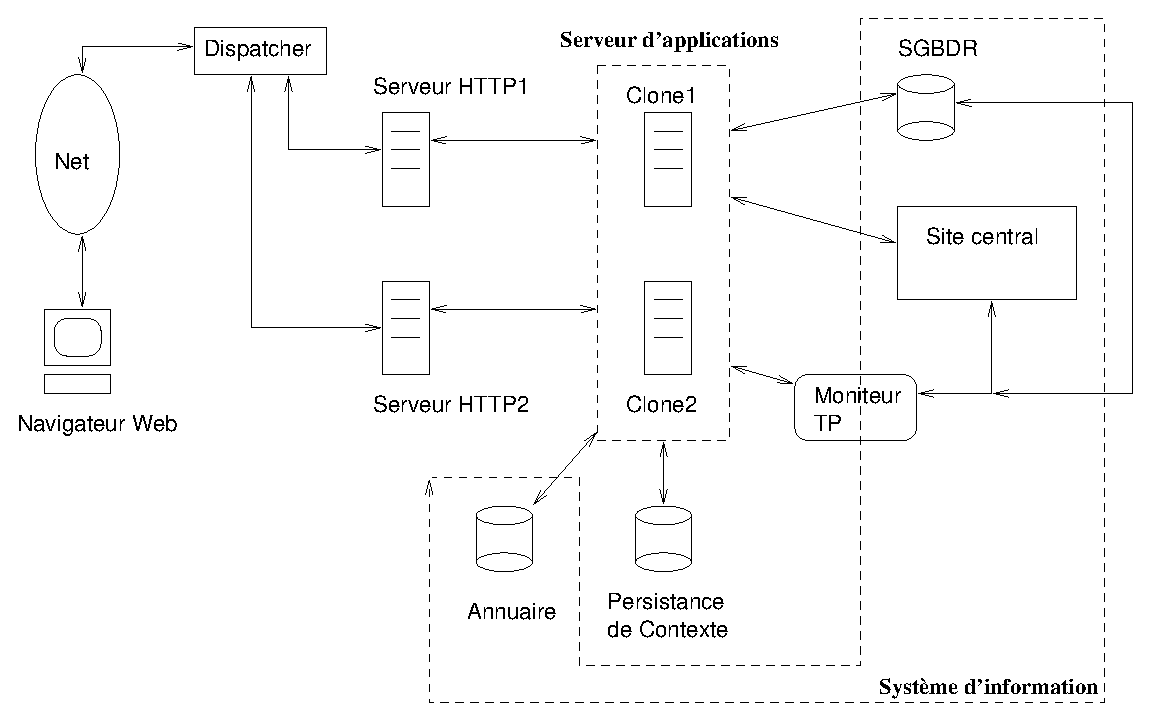
\epsfig{width=.9\textwidth,file=figures/fig-infra-technique.eps}
    \caption{Architecture technique}
    \label{fig-infra-technique}
\end{figure}

La communication avec le client est g\'er\'ee par un ou plusieurs
serveurs HTTP avec un r\'epartiteur de charge permettant de minimiser
temps de r\'eponses et trafic r\'eseau. Le serveur \textsf{HTTP}
communique avec le \emph{serveur d'applications} g\'en\'eralement au
travers d'un protocole ad-hoc, serveur qui peut \^etre clon\'e de
sorte que l\`a aussi, la charge soit r\'epartie sur plusieurs
machines et la tol\'erance aux pannes soit am\'elior\'ee.  Le
contexte, c'est \`a dire l'ensemble des informations relatives \`a
une session, est persistant selon un m\'ecanisme
propre au serveur
d'applications choisi. Les besoins d'authentification des clients,
qu'ils soient r\'ealis\'es par mots de passe ou par une
infrastructure \`a cl\'es publiques (\textsf{PKI}), sont
le plus souvent g\'er\'es par un annuaire d'entreprise de type
\textsf{LDAP}. Il en va de m\^eme pour l'habilitation des
utilisateurs, c'est \`a dire pour la d\'efinition de leurs droits
d'acc\`es sur les fonctions du syst\`eme. Notons que
l'authentification se fait g\'en\'eralement au niveau des serveurs
HTTP tandis que l'habilitation se fait dans le serveur d'applications. 

Le serveur d'applications contient l'ensemble de la logique  de
l'application (voir ci-dessous) et a la charge de communiquer au
travers de connecteurs idoines avec le reste du syst\`eme
d'information : bases de donn\'ees relationnelles, sites centraux,
moniteurs transactionnels. L'architecture \textsf{J2EE} pr\'evoit, au travers
des connecteurs \textsf{JCA}, la possibilit\'e de relier un tel
syst\`eme \`a n'importe quel autre  en maintenant des
propri\'et\'es transactionnelles. Pour une pr\'esentation
g\'en\'erale de l'architecture de la plateforme \textsf{J2EE}, voir
la section \ref{sec:j2ee} du chapitre \ref{chap-etatart}.

\subsection{Architecture logicielle}
\label{sec:arch-logic}
L'architecture logicielle utilis\'ee est une architecture en couches 
qui reprend un certain nombre de \og bonnes pratiques\fg{} d\'esormais
courantes dans le domaine. Elle s'inspire  de
\emph{patrons de conceptions}\cite{core-j2ee-patterns,gof} usuels, tels que le patron
\emph{Mod\`ele-Vue-Contr\^oleur} popularis\'e par le framework
\textsf{Struts} pour la gestion des interactions avec le client, ou
le patron \emph{Recherche de Services}  --- 
\emph{Service Locator} --- pour la localisation d'interfaces
m\'etiers offertes par les \textsf{EJB}. La figure
\ref{fig-archi-couche} reprend les diff\'erents \'el\'ements de
mani\`ere synth\'etique. 

\begin{figure}[htbp]
    \centering
    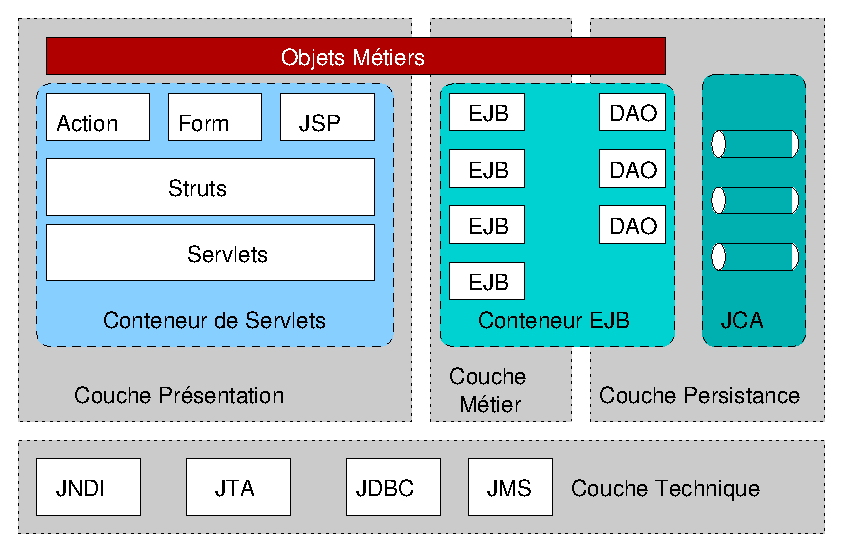
\epsfig{width=.9\textwidth,file=figures/fig-archi-couche.eps}
    \caption{Architecture logicielle}
    \label{fig-archi-couche}
\end{figure}

La \emph{couche pr\'esentation} s'appuie sur des \emph{servlets}
encapsul\'ees dans un conteneur, qui
permettent de d\'evelopper des contenus dynamiques en
\textsf{Java} en s'abstrayant d'un certain nombre de d\'etails
techniques tels que la gestion de la transformation des param\`etres
--- \emph{marshalling} --- depuis ou vers le protocole \textsf{HTTP},
la gestion du contexte de session et du contexte applicatif et surtout
la communication par appels de m\'ethodes distants avec la couche
m\'etier, c'est \`a dire les
\textsf{EJB}. \textsf{Struts} fournit
un canevas pour g\'erer les interactions avec le client et sur cette
base sont d\'evelopp\'es des \emph{actions}, des \emph{formulaires}
--- \emph{forms} --- et des \textsf{JSP} --- \emph{Java Server Pages}
--- repr\'esentant respectivement la partie contr\^ole, mod\`ele
et vue du patron \textsf{MVC}. 

La \emph{couche m\'etier} contient les \emph{Enterprise Java Beans},
un ensemble de services m\'etiers utilis\'es par la couche
pr\'esentation en fonction des besoins de l'application. Ces
\textsf{EJB} sont le plus souvent de type \emph{Session sans \'etat}
et le traitement de l'acc\`es aux donn\'ees est d\'el\'egu\'e
\`a des objets sp\'ecialis\'es appel\'es \emph{Data Access
  Objects} ou \textsf{DAO}, plut\^ot que laiss\'e \`a la
discr\'etion du conteneur et d'\textsf{EJB} \emph{Entit\'es}. 

La couche persistance est souvent la plus technique et la plus
d\'elicate. Dans l'id\'eal, elle r\'ealise une simple projection du
mod\`ele de classes des objets m\'etiers depuis ou vers un syst\`eme de base
de donn\'ees quelconque, ce qui peut \^etre fait de mani\`ere
automatis\'ee en s'appuyant sur un framework tel que les EJB
\emph{Entit\'es} ou \textsf{Hibernate}. Dans la pratique, compte tenu du fait
que les sch\'emas de table sont g\'en\'eralement pr\'eexistants
aux applications d\'evelopp\'ees, que les canevas de projection
objet-relationnel automatis\'es ont du mal \`a optimiser
correctement les transactions et les requ\^etes et que l'on a pas
uniquement affaire \`a des syst\`emes relationnels mais aussi
\`a des applications l\'egataires, \`a des transactions stock\'ees
\textsf{COBOL} ou encore \`a des couches de moniteurs transactionnels
propri\'etaires, cette gestion est le
plus souvent d\'evelopp\'ee de mani\`ere ad-hoc. 

La couche transversale \emph{objets m\'etiers} contient l'ensemble
des objets du domaine applicatif, autrement dit l'instantiation du
diagramme de classes des donn\'ees manipul\'ees par
l'application. Ces objets sont utilis\'es par toutes les couches, l'utilisation
d'objets dans les interactions entre couches permettant par ailleurs de
r\'eduire le nombre d'appels de m\'ethodes r\'ealis\'es et donc
d'accro\^{\i}tre les performances du syst\`eme. 

La couche technique, enfin, comprend un certain nombre de services sur
lesquels s'appuient les diff\'erents composants du syst\`eme :
\begin{itemize}
  \item service de nommage --- \emph{Java Naming and Directory
  Interface} ;
\item service de transaction --- \emph{Java Transaction API} ;
\item service d'acc\`es aux donn\'ees --- \emph{Java DataBase
    Connectivity} ;
\item service de messagerie asynchrone --- \emph{Java Message Service}.
\end{itemize}

\subsection{Processus de d\'eveloppement}

Le processus de d\'eveloppement utilis\'e est largement inspir\'e
du \emph{Rational Unified Process} ou \textsf{RUP}, m\^atin\'e d'une
bonne dose de pragmatisme et d'un zeste d'\emph{eXtreme
  Programming}. Nous renvoyons aux travaux r\'ealis\'es au sein de
l'entreprise par E.\textsc{Renaux}\cite{these-manu} pour une analyse
plus pouss\'ee de ce processus et de ses d\'efauts. 

Il s'agit l\`a d'un principe th\'eorique qui dans la  pratique
recouvre un d\'ecoupage plus \og traditionnel\fg{}  en activit\'es et
en lots :
\begin{itemize}
  \item les phases d'\emph{expression des besoins} et d'\emph{analyse} se confondent dans une
  m\^eme phase. Elles produisent un cahier des charges, des
  diagrammes de cas d'utilisation, des sc\'enarios  et des r\`egles
  m\'etiers ;
\item la \emph{conception} produit les
  diagrammes de classes et \'eventuellement d'\'etats-transitions
  associ\'es, ainsi que les sch\'emas de donn\'ees ;
\item le \emph{d\'eveloppement} r\'ealise effectivement
  l'application \`a partir des documents de conception ;
\item la phase de test ou phase de \emph{recette} valide l'application
  produite par rapport aux besoins initiaux.
\end{itemize}
Les it\'erations et incr\'ements  ont une granularit\'e beaucoup
plus grande que dans les pr\'econisations des m\'ethodes cit\'ees,
un probl\`eme  important dont on verra par la suite qu'il
d\'ecoule de carences dans la mod\'elisation de l'architecture
globale de l'application.

Le processus de d\'eveloppement s'appuie par ailleurs sur une analyse
d'\emph{urbanisation} du syst\`eme d'informations qui permet de
d\'ecouper globalement les processus m\'etiers en diff\'erents
\emph{quartiers} et \emph{blocs} reproduisant au niveau informatique
l'organisation du client.  Le processus tel que nous le pr\'esentons
ici doit \^etre compris comme une synth\`ese d'un ensemble de
pratiques dans diff\'erents contextes.  

\subsection{M\'ethodologie d'analyse \& conception}

La m\'ethodologie articule la conception en \emph{couches} et le
r\'esultat du processus d'analyse en \emph{vues}. Les diff\'erentes
couches recens\'ees sont:
\begin{itemize}
\item la couche \emph{Pr\'esentation} qui contient essentiellement les
\'el\'ements r\'egissant les interactions avec l'utilisateur :
description de l'interface graphique, r\`egles de navigation entre
\'ecrans ;
\item la couche \emph{Dynamique applicative} qui contient les processus de
l'application proprement dite, c'est \`a dire essentiellement les
actions \textsf{Struts} ;
\item la couche \emph{M\'etier} qui d\'efinit et contient les services
m\'etiers et les objets associ\'es ;
\item la couche \emph{Persistance} qui d\'ecrit les r\`egles d'interaction
entre objets-m\'etiers et syst\`eme de stockage.
\end{itemize}

Le processus d'analyse et de conception est d\'ecoup\'e en vues qui
sont chacune repr\'esent\'ees par diff\'erents mod\`eles \textsf{UML} et
\'el\'ements de documentation. Ces diff\'erentes vues sont:
\begin{itemize}
\item la \textbf{vue utilisateur} qui d\'ecrit les besoins de l'utilisateurs en
termes g\'en\'eraux ;
\item la \textbf{vue processus} qui mod\'elise chaque processus d'interaction
entre un utilisateur et le syst\`eme ;
\item la \textbf{vue composant} qui identifie les composants du syst\`eme,
leur fonctionnement et leur interaction avec d'autres composants ;
\item la \textbf{vue persistance} qui d\'ecrit les r\`egles de projection
entre objets-m\'etiers et syst\`eme de stockage persistant.
\end{itemize}

Nous d\'ecrivons succintement
chacune des vues dans les sections ci-dessous en proposant
syst\'ematiquement une synth\`ese sous la forme d'un
\emph{m\'eta-mod\`ele} \textsf{UML} de chaque vue.

\subsubsection{Vue utilisateur}

Les besoins utilsateurs sont d\'ecrits sous la forme de diagrammes de cas
d'utilisation et de diagrammes de classes. Un m\'eta-mod\`ele de
cette vue utilisateur est donn\'e ci-dessous (partie sup\'erieure de la
figure \ref{fig-vue-utilisateur}).

\begin{figure}[htbp]
    \epsfig{width=.60\textwidth,file=figures/vue-util-mm.eps}\hfill\epsfig{width=.60\textwidth,file=figures/vue-proc-mm.eps}
\centering
    \caption{Vues utilisateurs \& m\'etiers}
    \label{fig-vue-utilisateur}
\end{figure}

Dans cette vue, on exprime les besoins de l'utilisateur, d\'efinit
le p\'erim\`etre du syst\`eme, les interactions avec les
diff\'erents r\^oles de l'utilisateur. Cette vue permet de
d\'egager des \textbf{entit\'es fonctionnelles} (domaines)
repr\'esent\'ees dans le m\'eta-mod\`ele par une classe dont les
attributs sont d\'efinis par les cas d'utilisation.

\subsubsection{Vue Processus}

Cette vue, \`a partir des besoins utilisateurs exprim\'ees
pr\'ec\'edemment, va d\'efinir pr\'ecis\'ement les interactions
existant entre les diff\'erents r\^oles (acteurs) intervenant dans
l'application et  le syt\`eme. Ces interactions sont
repr\'esent\'ees dans une diagramme de cas d'utilisation, chaque cas
d'utilisation se trouvant par la suite associ\'e \`a un ou plusieurs
diagrammes d'activit\'e. Les regroupements de cas d'utilisation
repr\'esentent en fait des menus/actions acccessibles par
diff\'erents r\^oles du syst\`eme et leur organisation.

Cette vue permet en particulier d'indentifier et de caract\'eriser
les objets \textsf{IHM} utilis\'es (types d'\'el\'ements d'interfaces,
ordres de navigation, accessibilit\'e) et de d\'efinir les processus m\'etiers,
c'est \`a dire de documenter les algorithmes relatifs \`a chaque
\verb|Action| : quelles sont les \'el\'ements de donn\'ees de
l'\textsf{IHM} qui sont transmis et quels sont les r\'esultats ?

\subsubsection{Vue Composants}

La vue \og composants\fg{} d\'etaille:
\begin{itemize}
\item les \'el\'ements d'\textsf{IHM}, plus
particuli\`erement du point de vue de la couche dynamique
applicative, c'est \`a dire du \emph{serveur d'application} dans
l'architecture choisie ;
\item les services m\'etiers, c'est \`a dire les objets et leurs
interfaces permettant de r\'ealiser les fonctions demand\'ees par
l'utilisateur.
\end{itemize}

\begin{figure}[htbp]
    \epsfig{width=.60\textwidth,file=figures/vue-comp-mm.eps}\hfill\epsfig{width=.60\textwidth,file=figures/vue-pers-mm.eps}
\centering   
    \caption{Vue composants m\'etiers \& persistance}
    \label{fig-vue-composant}
\end{figure}

Le diagramme d'activit\'e issu de la phase pr\'ec\'edente est
enrichi par des informations suppl\'ementaires sur les \'el\'ements
concrets de r\'ealisation des classes \verb|IHM|  (maquette HTML, page
JSP, attributs) et des \'el\'ements \verb|Flux d'objet|. Ces flux
d'objets correspondent \`a des invocations de services m\'etiers
(BO) ou d'\'el\'ements de l'infrastructure logicielle sous-jacente
(API). \`A chaque transition d\'eclench\'ee par une activit\'e
d'IHM correspond une m\'ethode dans la classe d'IHM correspondante,
m\'ethode qui sera document\'ee en d\'ecrivant les contr\^oles
effectu\'es sur les attributs de l'objet.

\subsubsection{Vue M\'etier/persistance}

Cette derni\`ere vue d\'efinit plus pr\'ecis\`ement les objets
m\'etiers et la mani\`ere dont ces objets sont stock\'es et
correspondent \`a des donn\'ees pr\'esentes dans des applicationss
patrimoniales (sites centraux), des SGBD ou toute autre forme de
projection. Comme indiqu\'e dans le paragraphe pr\'ec\'edent,
les objets BO et API ont pour fonction de faire le lien entre les
services vus du point de vue de l'application et les donn\'ees et
couches techniques.  Des r\`egles d'acc\`es aux
donn\'ees persistantes sont par ailleurs d\'efinies \`a ce stade mais nous avons
choisi de ne pas les analyser dans ce document. Nous  consid\'erons
en effet  qu'il s'agit de probl\`emes de l'ordre de l'implantation et des choix
technologiques r\'ealis\'es qui ne doivent pas avoir d'impact sur
les \textbf{fonctionnalit\'es}  de l'application.

\subsection{Infrastructure de d\'eveloppement}

Les d\'eveloppements s'appuient sur un certains nombres d'outils et
de pratiques ayant pour objectif d'accro\^{\i}tre la qualit\'e et la
fiabilit\'e du r\'esultat final. D'une part, ils s'appuient sur une
d\'emarche globale d'\emph{ing\'eni\'erie dirig\'ee par les
  mod\`eles} permettant de tirer partie de l'existence de mod\`eles
de conception et de lib\'erer le d\'eveloppeur des contraintes
techniques induites par la plateforme. Concr\`etement, cela signifie
qu'\`a partir des diagrammes de classes des objets m\'etiers, on utilise des outils de g\'en\'eration de code pour
produire automatiquement les \'el\'ements n\'ecessaires \`a
l'infrastructure technique : interfaces distantes et fabriques dans le
cas des \textsf{EJB}, fichiers de configurations \textsf{XML} pour la
persistance des donn\'ees et la couche pr\'esentation, formulaires
\textsf{Struts}.

D'autre part, un processus d'\emph{int\'egration continue} pilot\'e
par \textsf{Maven} et bas\'e
sur un \emph{syst\`eme de gestion de versions} permet d'automatiser
la construction des d\'elivrables de l'applications --- paquetages,
archives, descripteurs de d\'eploiement ---- et surtout de produire
\`a intervalles r\'eguliers une photographie de l'ensemble de
l'application, de sa documentation et une batterie de
v\'erifications statiques et dynamiques. Ce principe est r\'esum\'e
dans la figure \ref{fig-develmvc} et reprend la forme d'un patron
\textsf{MVC} dans lequel les vues sont les diff\'erentes phases ou
acteurs du processus de d\'eveloppement, le contr\^oleur est le
moteur d'int\'egration continue et le mod\`ele est le syst\`eme de
gestion de configurations.  

\begin{figure}[htbp]
    \centering
    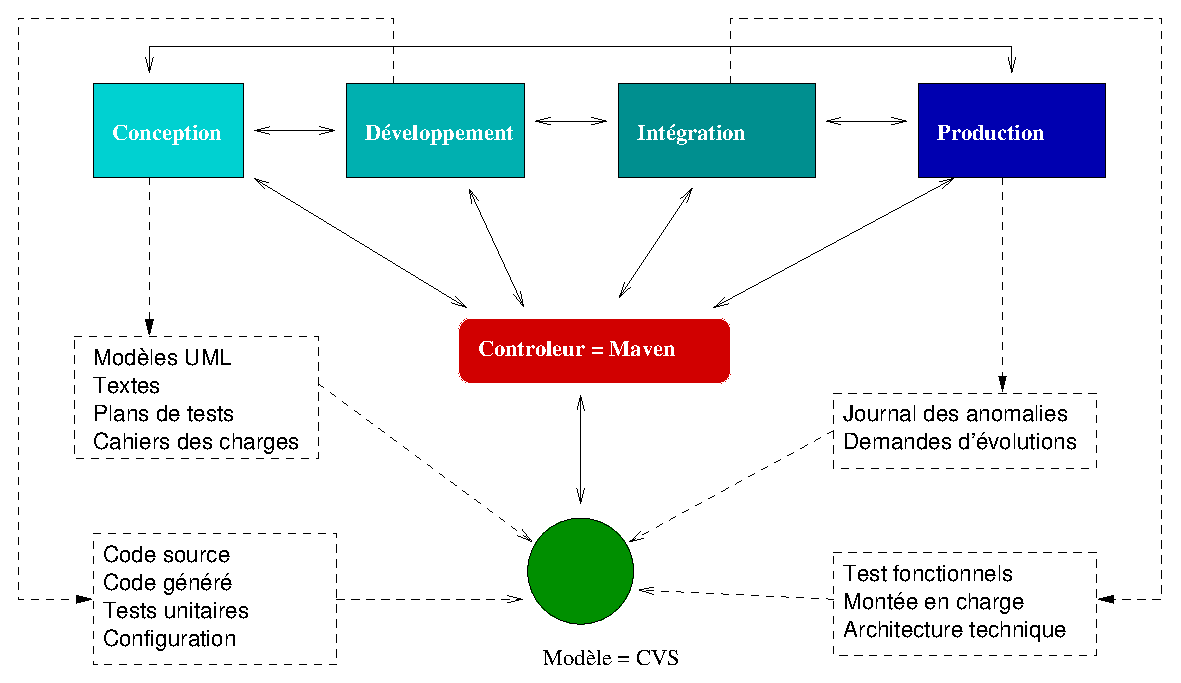
\epsfig{width=.8\textwidth,file=figures/fig-develmvc.eps}
    \caption{Mod\`ele de processus de d\'eveloppement}
    \label{fig-develmvc}
\end{figure}

Les v\'erifications r\'ealis\'ees par le contr\^oleur \`a partir
du code source sont les suivantes :
\begin{itemize}
  \item v\'erifications des r\`egles syntaxiques de codage : nommage
  des entit\'es dans le code, indentation et formatage, ... ;
\item v\'erifications de r\`egles --- simples --- de s\'emantique :
  code mort, variables inutilis\'ees et d\'eclarations incorrectes,
  ... ;
\item calculs de m\'etriques par paquetage telles que le degr\'e
  d'abstraction/concr\'etion, le taux de couplage, le degr\'e de
  complexit\'e, ... ;
\item v\'erification des r\`egles d'acc\`es architecturales entre
  classes et paquetages permettant de v\'erifier le respect par les
  d\'eveloppeurs de l'architecture globale  du syst\`eme ;
\item ex\'ecution des tests unitaires et calcul de la couverture de
  code --- instructions et branchements --- r\'ealis\'ee.
\end{itemize}

Le d\'eveloppement et la mise en \oe uvre de ces outils a
constitu\'e une part importante  de notre contribution au sein de
l'entreprise et s'est \'etal\'ee sur diff\'erents projets. En l'\'etat actuel des choses, seule la
vue \emph{D\'eveloppement} est r\'eellement op\'erationnelle. Une
partie de l'objectif de cette th\`ese est de faire en sorte que les
autres vues, et plus particuli\`erement les vues \emph{Conception} et
\emph{Int\'egration} soient misent en places par la gestion
automatis\'ee des tests fonctionnels \`a diff\'erents niveaux de
l'architecture et la validation crois\'ee entre mod\`eles et
sources. 

\section{Analyse critique}
\label{sec:analyse-critique}
Apr\`es un rapide tour d'horizon du processus de d\'eveloppement
type d'applications r\'eparties sur architecture \textsf{J2EE} tel
que nous le pratiquons aujourd'hui, cette section est consacr\'ee
\`a une analyse critique dudit processus en partant des probl\`emes
constat\'es concr\`etement lors de la vie des projets et des
\'el\'ements m\'ethodologiques pr\'esent\'es. 

Comme l'a fort bien soulign\'e E.\textsc{Renaux} dans ses travaux
pr\'ec\'edemment cit\'es, un des probl\`emes essentiels auquel
nous sommes confront\'es est le passage de l'\emph{analyse} \`a la
\emph{conception}, c'est \`a dire la transformation d'un sch\'ema de
compr\'ehension g\'en\'eral du processus m\'etier de l'application
en un mod\`ele de conception \`a base de composants. La propositon
\emph{Component Unified Process}\cite{manu-cup-lmo,these-manu} a pour objectif de r\'esoudre ce
probl\`eme en introduisant au plus t\^ot une structuration en
composants des diff\'erentes fonctionnalit\'es de
l'application. Notons que c'est partiellement ce qui est
pr\'econis\'e dans le processus de mod\'elisation que nous avons
d\'etaill\'e ci-dessus. 

Nous nous int\'eressons toutefois \`a un probl\`eme diff\'erent :
il s'agit, rappelons-le, de v\'erifier que ce qui est d\'evelopp\'e
correspond bien \`a ce qui est attendu, pas plus, pas moins. Notre
analyse sera donc sous-tendue par cette probl\'ematique.

\subsection{Complexit\'e}

Les syst\`emes d'information en particulier, et les gros syst\`emes
informatiques en g\'en\'eral, ont toujours \'et\'e complexes mais
cette complexit\'e conceptuelle se trouve aujourd'hui
d\'emultipli\'ee par la complexit\'e des architectures techniques
et applicatives mises en place. L'h\'et\'erog\'en\'eit\'e des
syst\`emes, la r\'epartition des processus, l'omnipr\'esence des
r\'eseaux, rendent la t\^ache du concepteur et du d\'eveloppeur
encore plus complexe. Le \og paradigme \fg{} de programmation
orient\'ee-objet n'a rien r\'esolu, bien au contraire, puisqu'il
exige de distribuer non seulement les processus de traitements
informatiques eux-m\^emes mais aussi les processus m\'etiers. 

Les plateformes de composants n'ont pas beaucoup mieux r\'eussi \`a
simplifier le probl\`eme et ont m\^eme plut\^ot accru la
fragilit\'e des applications en les rendant d\'ependantes de
services techniques. Ces derniers sont  parfois difficiles \`a appr\'ehender et toujours
d\'elicats \`a int\'egrer dans une conception de par la
multiplication des fichiers de configurations divers et des
contraintes de programmation et de conception.
Les ateliers de d\'eveloppement, s'ils permettent d'all\'eger
certaines t\^aches, ne r\'esolvent pas tout. 

\subsection{Coh\'erence des \'el\'ements du d\'eveloppement}

Le processus de d\'eveloppement, \`a partir de l'expression des
besoins, n'est absolument pas incr\'emental ni it\'eratif
mais est bien plus proche d'un mod\`ele en cascade traditionnel : les
phases d'analyse, de conception et de d\'eveloppement s'encha\^{\i}nent
dans un ordre descendant mais sans que l'information ne puisse
remonter la \og cascade\fg{}. Au final, il est fr\'equent que les
documents d'analyse et de conception soient obsol\`etes lors de la
livraison. Au mieux, ils sont \'ecrits \`a posteriori en
fonction du code effectivement livr\'e. 

Ce probl\`eme provient de
l'absence de lien direct et surtout automatis\'e avec la r\'ealisation
concr\`ete du logiciel, autrement dit du d\'ecouplage entre les
mod\`eles et le code. M\^eme dans les domaines o\`u le code est
g\'en\'er\'e \`a partir de mod\`eles, l'information est \`a sens
unique et il difficile d'int\'egrer \`a la fois les
d\'eveloppements manuels et la production automatis\'ee d'une partie
du code. 

Au sein des phases d'analyse et de conception elles-m\^emes, la
coh\'erence entre les mod\`eles et le respect d'un certain nombre de
r\`egles g\'en\'erales ne sont pas syst\'ematiquement
v\'erifi\'es. 

Enfin, nombre de d\'eveloppements sont des red\'eveloppements. On
suppose donc que le travail d'analyse a d\'ej\`a \'et\'e fait et
on en fait l'\'economie. Malheureusement, les processus \'evoluent
aussi et sont rarement ind\'ependants des technologies de leur mise
en \oe uvre. Les documents sur lesquels sont bas\'es des
red\'eveloppements sont donc souvent obsol\`etes, incomplets voire
faux, d'o\`u l'impossibilit\'e de valider les logiciels produits \emph{a
priori} et de mani\`ere m\'ecanique.

\subsection{Interp\'en\'etration des domaines}

Les fonctionnalit\'es de l'application se trouvent
souvent m\'elang\'ees \`a des \'el\'ements r\'eglant la navigation et
l'acc\`es de l'utilisateur \`a ces diff\'erentes fonctions. C'est
particuli\`erement le cas dans les \'el\'ements
d'\textsf{IHM}, qui m\'elangent niveaux de validation et r\`egles de
navigation. Il nous semble qu'il s'agit de probl\`emes strictement orthogonaux :
\begin{itemize}
\item l'application offre la possibilit\'e \`a l'utilisateur de
r\'ealiser certaines op\'erations, ce sont les services
offerts. Leur encha\^{\i}nement, leur structure, leurs besoins, l'algorithmique
sont d\'etaill\'es par les diff\'erents documents d\'ecrivant
les processus et le m\'etier. En particulier, les encha\^{\i}nements
de processus n\'ecessaires ou possibles sont mod\'elis\'es sous la
forme de diagrammes d'activit\'es ou automates d'\'etats finis ;
\item l'\textsf{IHM} est une \emph{traduction} \`a l'usage des op\'erateurs humains
interagissant avec le syst\`eme du comportement attendu du
syst\`eme. En particulier, les encha\^{\i}nements impos\'es et les
actions activ\'ees et inactiv\'ees du syst\`eme en fonction de
l'\'etat de l'activit\'e se trouvent r\'ealis\'ees graphiquement
par des modifications d'\'ecran et d'attributs des \'el\'ements
composant l'\textsf{IHM}.
\end{itemize}

On retrouve le m\^eme probl\`eme dans la couche
composants/persistance. Le probl\`eme de la persistance des objets
m\'etiers se trouve trait\'e au m\^eme niveau que celui de leur
d\'efinition et de leur manipulation. Des objets purement
m\'ecaniques  tels que les \emph{objets donn\'ees} se trouvent
pr\'esents dans la mod\'elisation alors m\^eme qu'ils sont
automatiquement g\'en\'er\'es par des r\`egles de projection. Enfin, la structure des tables relationnelles se trouve reproduite,
avec tous les probl\`emes que cela comporte, dans le mod\`ele qui de
facto perd ainsi sa structure objet.

\subsection{Formalisation}

Les mod\`eles d'analyse et de conception ne sont pas tels
quels v\'erifiables automatiquement. Leur coh\'erence est assur\'ee par des
r\`egles de nommage qui ne sont pas toujours respect\'ees \`a la
lettre, la dynamique et les algorithmes sont document\'es en
commentaires sous la forme de pseudo-code non formalis\'e et donc non
ex\'ecutable par un compilateur, les mod\`eles d'analyse (diagrammes
d'activit\'es) ne sont pas suffisamment pr\'ecis pour permettre de
d\'eriver automatiquement des sc\'enarios de tests (quand bien
m\^eme ceci est pr\'evu dans le processus, voir ci-dessus).

La structure des mod\`eles n'est pas suffisamment congruente
avec l'architecture finale, ni li\'ee au code d\'evelopp\'e, pour
permettre de faire des liens et d\'eductions automatiques et
g\'en\'erer \'eventuellement des squelettes de tests unitaires. Ces
mod\`eles ne sont pas maintenus d'une \'etape \`a une autre, ce
qui produit donc des d\'erives entre phases qui rendent rapidement la
t\^ache de g\'en\'eration automatique impossible. La production de
tests unitaires pour les diff\'erents composants du syst\`eme est
ainsi rendue plus difficile car elle n\'ecessite de la part des
\'equipes de d\'eveloppement de se plonger dans les d\'etails de
la documentation d'analyse et de conception pour \'evaluer les
fonctionnalit\'es attendues de tel ou tel objet. 

Cette absence de formalisation est aussi un probl\`eme aux deux bouts
de la cha\^{\i}ne puisque les impr\'ecisions dans l'expression des
besoins et l'analyse des fonctionnalit\'es de l'application rendent
tr\`es difficile la mise en en \oe uvre de strat\'egies de tests
syst\`emes et d'int\'egration efficaces pour am\'eliorer la
qualit\'e de l'application avant le passage en recette. Un grand
nombre d'erreurs triviales sont ainsi rep\'er\'ees, parfois avec
difficult\'e, lors de cette phase de recette alors qu'elles auraient
pu \^etre d\'etect\'ees plus t\^ot. 

\subsection{Architecture}

Le gros point noir du processus de d\'eveloppement, duquel
d\'ecoule une grande partie des autres probl\`emes, est l'absence
d'un mod\`ele global d'architecture de l'application et d'un
d\'ecoupage clair de celle-ci \`a diff\'erents niveaux de
d\'etails. Bien s\^ur, cette architecture existe et le d\'ecoupage
r\'ealis\'e lors de la r\'ealisation du cahier des charges et/ou de
l'urbanisation du syst\`eme d'information est repris lors des phases
du d\'eveloppement. 

Mais aucun mod\`ele n'offre une vue d'ensemble synth\'etique du
syst\`eme, ni la possibilit\'e de visiter les \'el\'ements du
syst\`eme de mani\`ere hi\'erarchique ou th\'ematique : par
couches ou par domaine fonctionnel. Les diff\'erents mod\`eles sont d\'ecoup\'es en fonction des
phases du processus, et nous l'avons vu, il n'est pas pr\'evu la
possibilit\'e de revenir sur des diagrammes plus abstraits en
fonction de choix et de d\'ecouvertes faits \`a des niveaux plus
concrets.

Le r\'esultat net est une extraordinaire complexit\'e des mod\`eles
dans les d\'etails desquels l'utilisateur se trouve tr\`es
rapidement noy\'e. Cette complexit\'e est mieux ma\^{\i}tris\'ee dans
le code \'ecrit qui se trouve structur\'e de mani\`ere plus
\'evidente et pour lequel les outils de construction offrent une vue
synth\'etique rapide.

Alors m\^eme que l'on parle beaucoup de composants, tant pour ce qui
concerne les plateformes que pour la structuration des applications et
du processus de d\'eveloppement, on se rend compte que ces composants
n'existent pas au niveau de l'analyse et de la conception. Dans les
d\'eveloppements, seuls les composants impos\'es par
l'infrastructure techniques apparaissent : \textsf{EJB},
\textsf{Servlets}, \'eventuellement connecteurs
\textsf{JCA} pour la couche persistance. Rien dans les
mod\`eles d'analyse ou de conception ne permet de d\'eduire une
structure compositionnelle de l'application : il n'y a pas de
d\'efinition explicite de composants ni de composites, pas de
notions de ports interconnect\'es, pas de sch\'ema d'architecture
repr\'esentant les diff\'erents composants et leurs interactions.

\section{Pr\'econisation}

Il n'y a bien s\^ur pas de solution unique pour r\'esoudre cet
ensemble de probl\`emes, et il est m\^eme certain qu'il est
impossible de les r\'esoudre compl\'etement, mais l'exp\'erience
m\^eme de \textsf{Norsys} sur d'autres technologies a montr\'e qu'il
\'etait possible d'\emph{industrialiser} les d\'eveloppements pour
accro\^{\i}tre leur qualit\'e et leur productivit\'e. Nous avons
d\'ej\`a signal\'e les travaux d'E.\textsc{Renaux} sur le
\emph{Processus Unifi\'e de Composants} --- \textsf{CUP}
---\cite{manu-cup-lmo} r\'ealis\'es dans le cadre d'une collaboration avec
Norsys. 

Le point cl\'e de cette d\'emarche consiste \`a identifier les
composants le plus t\^ot possible, d\`es la mod\'elisation des
exigences de l'utilisateur au travers des \emph{cas
  d'utilisation}. Cette identification pr\'ecoce permet 
 d'assurer lors des phases ult\'erieures de conception et de
d\'eveloppement un suivi continu. Cette approche est
articul\'ee autour de la notion de composant logique correspondant
\`a un m\'eta-mod\`ele et concr\'etis\'ee en quatre vues
compl\'ementaires bas\'ees sur ce m\'eta-mod\`ele :
\begin{enumerate}
  \item la vue des cas d'utilisation ;
  \item la vue d'interactions ;
  \item la vue de conception ;
  \item et la vue d'assemblage. 
\end{enumerate}

D'autre travaux de recherche sont en cours dans l'entreprise
sur les probl\`emes de la r\'eing\'enierie d'applications
patrimoniales --- J.\textsc{Hattat} --- et de la s\'eparation des
pr\'eoccupations par des \emph{aspects} de conception ---
D.\textsc{Diaz}. 

De notre c\^ot\'e, nous avons focalis\'e notre travail sur les deux
points suivants :
\begin{itemize}
  \item la mise en place d'une \emph{architecture \`a base de
    composants contractualis\'es}
    depuis l'analyse jusqu'\`a la r\'ealisation ;
  \item l'am\'elioration de la qualit\'e des dits composants par la
    g\'en\'eration automatis\'ee de tests fonctionnels.
\end{itemize}

\subsection{Pour une architecture des logiciels}

Le meilleur processus de fabrication non informatique auquel on peut comparer la
conception et la r\'ealisation d'un syst\`eme d'information est
celui de la conception et de la r\'ealisation d'un b\^atiment ou
d'un ouvrage d'art. Dans chacun des cas :
\begin{itemize}
  \item le produit final est unique ;
  \item  il fait appel \`a la comp\'etence
    d'une multitude de m\'etiers ;
  \item  il n\'ecessite une vision \`a la
    fois g\'en\'erale et d\'etaill\'ee ;
  \item  il est soumis aux m\^emes
    contraintes dans ses rapports avec l'utilisateur, contraintes exprim\'ees
    au travers d'un cahier des charges ;
  \item  son r\'esultat ne  peut-\^etre \'evalu\'e \emph{in fine} que par l'usage qui en
    est fait ;
  \item  il peut s'inscrire dans un ensemble pr\'e-existant ou
    \^etre con\c{c}u \emph{ex nihilo} ;
  \item  il peut produire un r\'esultat dont la qualit\'e va de d\'esastreuse --- le terminal T3 de
    l'a\'eroport Roissy-Charles-de-Gaulle ou la premi\`ere
    version d'\textsf{Amadeus}, le syst\`eme de r\'evervation de la
    \textsf{SNCF} --- \`a admirable --- Taliesin par Frank Lloyd Wright ou le
    syst\`eme d'exploitation \textsf{Unix} ;
  \item  il peut \^etre pr\'evu    pour durer --- la cath\'edrale de Chartres ou Internet --- ou
    \^etre jetable ;
  \item  les deux march\'es repr\'esentent des tailles
    comparables et consid\'erables --- \$3500 milliards pour le
    g\'enie civil, \$1322 milliards pour les services des
    technologies de l'information ;
  \item enfin, il rentre dans le jugement que l'on
    peut en faire une part essentielle de crit\`eres esth\'etiques.
\end{itemize}
De cette analogie, on peut inf\'erer que le concept central au c\oe
ur  de l'activit\'e de conception et de r\'ealisation de logiciels
est celui d'\emph{architecture}. L'archictecture est ici comprise  non pas uniquement dans sa dimension
purement conceptuelle de production de formes, d'agencements de
structures et de r\'ealisation de plans, mais aussi dans sa dynamique
concr\`ete en tant que  point d'articulation entre les diff\'erents
acteurs d'un processus et leurs contraintes. 

Un composant est donc dans cette vision architecturale la
mat\'erialisation dans un plan plus large d'un concept et d'un
ensemble de contraintes, une partie d'un tout. Il  est 
n\'ecessairement d\'efini par les relations qu'il entretient avec
les autres composants du plan. De plus, un composant peut \^etre lui
m\^eme compos\'e de parties concourrant \`a la r\'ealisation de
ses fonctions. Une architecture est donc sym\'etriquement d\'efinie
comme un agencement de composants dans l'objectif de fournir un ensemble
de fonctionnalit\'es. Sans composants, pas d'architecture ; sans
architecture, pas de composants.

Nous n'avons pas la pr\'etention de penser que ce point
de vue soit original mais il nous para\^{\i}t essentiel, et c'est tout
l'enjeu de ce travail, de r\'eaffirmer son importance et surtout de
se donner les moyens de le rendre effectif.

\subsubsection{Compositionnalit\'e}

De toute \'evidence, les composants doivent pouvoir \^etre
compos\'es pour former \`a leur tour de nouveaux composants, plus
gros ou plus g\'en\'eraux. Inversement, un composant doit pouvoir
\^etre arbitrairement d\'ecompos\'e en divers constituants
permettant de d\'ecrire telle ou telle de ses fonctionnalit\'es. 

Toutes les exigences qu'un composant impose \`a son environnement
doivent \^etre explicitement sp\'ecifi\'ees. 
Les fonctionnalit\'es ainsi que les d\'ependances d'un composant doivent \^etre exprim\'ees
\emph{contractuellement}, en termes des relations qu'il entretient
avec son environnement et non pas en termes de la structure interne du composant.

Les relations que les composants entretiennent entre eux sont ainsi toujours
exprim\'es par des \emph{contrats bilat\'eraux} : un composant ne
peut subordonner l'ex\'ecution d'un service \`a la r\'ealisation
par un tiers d'un autre service ou d'une obligation d'un autre
contrat. De la sorte, tout composant devient substituable \`a un
autre pour autant qu'il remplisse chaque obligation contractuelle
substitu\'ee.

Ces relations contractuelles peuvent \^etre explicitement d\'ecrites
soit en tant que \emph{connecteurs}, auquel cas la s\'emantique des
relations entre composants est exog\`ene, soit intrins\`equement
lors de la mise en relation des composants. 

\subsubsection{Formalisation}

Le comportement d'un composant et la structure d'une architecture
doivent pouvoir \^etre d\'efinis formellement, c'est \`a dire
associ\'es \`a une s\'emantique non ambig\"ue et susceptible
d'\^etre v\'erifiable, m\^eme partiellement, par des moyens
m\'ecaniques. 
De m\^eme, une architecture donn\'ee --- un agencement de composants --- doit
pouvoir \^etre valid\'ee m\'ecaniquement en fonction de r\`egles
de coh\'erences g\'en\'erales. 

Il doit donc \^etre possible d'exprimer des propri\'et\'es et de
v\'erifier que ces propri\'et\'es sont bien pr\'esentes dans
l'architecture. Les propri\'et\'es exprimables doivent au minimum
\^etre les propri\'et\'es de \emph{s\^uret\'e}. 

Enfin, une architecture doit se pr\^eter \`a toute op\'eration de
\emph{raffinement} consistant \`a appliquer une transformation
produisant une nouvelle architecture correcte \`a un niveau
d'abstraction diff\'erent de l'architecture de d\'epart.

\subsubsection{Abstraction \& Concr\'etion}

Un composant doit \^etre une \emph{abstraction} ind\'ependante de toute
implantation mais susceptible de s'incarner dans la plus grande
palette possible de plateformes techniques, autrement dit un \emph{mod\`ele}. 
De plus, si un composant
est formellement sp\'ecifi\'e et ind\'ependant de toute plateforme,
il doit pouvoir \^etre \emph{r\'eifi\'e} m\'ecaniquement de sorte
que le r\'esultat soit par construction une implantation conforme et
ex\'ecutable.

De mani\`ere sym\'etrique, \'etant donn\'es un composant et une r\'ealisation concr\`ete
de ce composant, il doit \^etre possible de v\'erifier
m\'ecaniquement que la r\'ealisation concr\`ete est conforme aux propri\'et\'es
attendues du composant. 

Les donn\'ees, leur structure, leurs propri\'et\'es  et leurs
transformations constituant la majeure partie des fonctionnalit\'es
d'un syst\`eme d'information, leur d\'efinition et leur manipulation
doivent \^etre prises en compte dans la description des propri\'et\'es
des composants, ce \`a un niveau d'abstraction ad\'equat avec la
repr\'esentation du \emph{m\'etier} que ces \'el\'ements mod\'elisent.

\subsubsection{Synth\`ese}

En r\'esum\'e, nous attendons d'un mod\`ele d'architecture de
composants qu'il soit :
\begin{itemize}
  \item simple \`a manipuler avec un nombre de concepts restreints ;
  \item formel ;
  \item ex\'ecutable ;
  \item testable ;
  \item compositionnel et hi\'erarchique.
\end{itemize}

\subsection{Test \& Fiabilit\'e}

Pour s'assurer de la validit\'e d'un logiciel par rapport au cahier
des charges, on peut appliquer le principe des \emph{m\'ethodes
  formelles} : partir d'une expression formelle des exigences
en termes abstraits, et r\'ealiser, par des \'etapes de raffinement et
de preuve du maintien des invariants du niveau pr\'ec\'edent,
diff\'erents mod\`eles de plus en plus d\'etaill\'es, jusqu'\`a
obtenir un mod\`ele suffisamment pr\'ecis pour qu'il soit possible
de le projeter de mani\`ere non ambig\"ue vers un langage
d'implantation concret. C'est la strat\'egie de m\'ethodes telles
que \textsf{B}, \textsf{Z} ou \textsf{VDM}, illustr\'ee dans la
figure \ref{fig-process-b}.

\begin{figure}[htbp]
    \centering
    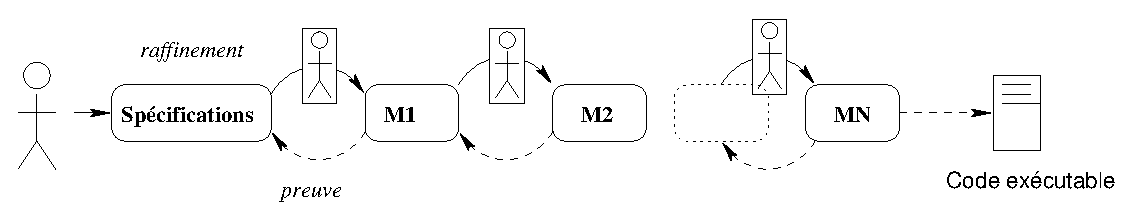
\epsfig{width=.8\textwidth, file=figures/fig-process-b.eps}
    \caption{D\'eveloppement formel par raffinement}
    \label{fig-process-b}
\end{figure}

Cette m\'ethode pr\'esente l'avantage \'evident de produire une application
dont la validit\'e eu \'egard aux sp\'ecifications est
\emph{prouv\'ee}, sous r\'eserve de la preuve de correction de la
projection terminale d'un mod\`ele en code. 

Une autre solution est, toujours \`a partir d'une expression formelle des
exigences, de produire automatiquement des \emph{cas de test} qui
permettront \`a l'issue du processus de d\'eveloppement  de valider
le logiciel produit : c'est ce qu'illustre la figure
\ref{fig-process-test}. 

\begin{floatingfigure}{.5\textwidth}
    \centering
    \epsfig{width=.45\textwidth, file=figures/fig-process-test.eps}
    \caption{D\'eveloppement formel par test}
    \label{fig-process-test}
\end{floatingfigure}

La premi\`ere solution est aujourd'hui inaccessible dans le contexte
qui est le notre, pour un certain nombre de raisons : le niveau de
fiabilit\'e exig\'e dans les applications de syst\`emes
d'informations est nettement moins \'elev\'e que dans des
syst\`emes critiques temps r\'eels ; le co\^ut de la mise en \oe
uvre de m\'ethodes formelles est tr\`es \'elev\'e, surtout compte
tenu du fait que la phase de preuve ne peut \^etre en l'\'etat
actuel des m\'ethodes et outils totalement automatis\'ee ;
l'int\'er\^et de mettre en place un tel processus dans des
syst\`emes h\'et\'erog\`enes en constante \'evolution para\^{\i}t
limit\'e. 

La seconde solution para\^{\i}t plus ais\'ee \`a mettre en place. Elle
exige toutefois un certain nombre de pr\'e-requis : l'existence d'une
sp\'ecification suffisamment formalis\'ee pour permettre la
d\'erivation automatique de cas de tests pertinents ; le maintien
d'une coh\'erence dans le processus de d\'eveloppement permettant de
faire en sorte que les cas de tests produits initialement restent
applicable \`a l'autre bout de la cha\^{\i}ne, c'est \`a dire lors de
la construction du logiciel fini ; l'existence de proc\'edures
automatiques fiables et de mesures de la fiabilit\'e atteinte par
l'ex\'ecution d'un ensemble donn\'e de tests. 

Le but de ce travail est donc de faire en sorte que ces deux solutions
au probl\`eme de la qualit\'e des logiciels produits : un processus
de d\'eveloppement centr\'e sur une architecture de composants
hi\'erarchiques, un processus de test automatis\'e et fiable, se
rejoignent.

%%% Local Variables: 
%%% mode: latex
%%% TeX-master: "these"
%%% TeX-master: "these"
%%% TeX-master: "these"
%%% End: 
    
\chapter{Architecture \& Composants}
\label{chap-etatart}
\citer{
\textbf{Architecture} : 1. Art, science et technique de la construction, de la
restauration, de l'am\'enagement des \'edifices. \emph{P. anal.} 
1. Principe d'organisation d'un ensemble, agencement, structure :
2. Ensemble structur\'e, organis\'e, construction \emph{Rem.} 1. Le
terme est employ\'e, tant sur le plan concr. que sur le plan abstr.,
dans des cas tr\`es divers o\`u il y a agencement, combinaison de
diff\'erentes parties pour former un tout, un ensemble homog\`ene,
organis\'e (ou paraissant l'\^etre) selon une certaine structure, un
certain plan. \'ETYMOL. ET HIST. Empr. au lat. architectura \og art
de construire \fg}{Tr\'esor de la Langue Fran\c{c}aise}


Nous avons dans le chapitre \ref{cha:proc-de-devol} insist\'e sur le
besoin d'une conception formalis\'ee de l'architecture des
logiciels. Nous avons aussi conclu que la notion d'architecture
\'etait li\'ee \`a la notion de composants. Ce chapitre sera donc
consacr\'e \`a ce qu'il est convenu d'appeler
l'\'etat de l'art dans le domaine de la mod\'elisation, de la
sp\'ecification et de la r\'ealisation d'architecture de syst\`emes
\`a base de composants.

Nous partirons des outils et plateformes orient\'ees-composant
concr\`etes, dans lesquelles un composant est une entit\'e
logicielle bien d\'efinie, s'ins\'erant dans un mod\`ele
d'ex\'ecution et de communication lui aussi pr\'ecis. Le
d\'eveloppement sur ces plateformes --- \textsf{J2EE},
\textsf{Corba}, \textsf{.Net} ---  constituent aujourd'hui l'essentiel
des d\'eveloppements dans les soci\'et\'es de services. Et nous
essayerons de comprendre pourquoi ces plateformes sont un \'echec
relatif en termes d'am\'elioration de la qualit\'e des logiciels. 

Ceci nous am\'enera naturellement \`a \'etudier un certain nombre
de propositions pour la conception d'architectures. \`A partir des
outils de mod\'elisation propos\'es autour du langage \textsf{UML},
nous nous int\'eresserons plus particuli\`erement aux nombreux travaux autour des \emph{Langages de
  Description d'Architecture} --- \textsf{ADL} en anglais. Sachant
qu'il existe d\'ej\`a des excellentes synth\`eses sur les ADL les
plus anciens, nous nous concentrerons sur quelques propositions plus 
r\'ecentes du domaine.

Enfin, nous aborderons certains mod\`eles plus th\'eoriques qui
s'int\'eressent \`a la composition de composants poss\'edant une
description comportementale formalis\'ee. 

\section{Plateformes de composants}

Une d\'efinition tr\`es fr\'equemment reprise du terme de composant
est celle propos\'ee  dans \cite{szyperski} (p.36, traduction par nos
soins) : 
\begin{quote}
    \og Un composant logiciel est une unit\'e de composition avec des
    interfaces contractuellement sp\'ecifi\'ees et des
    d\'ependances uniquement contextuelles. Un composant logiciel
    peut \^etre d\'eploy\'e de mani\`ere ind\'ependante et
    compos\'e par des \'el\'ements tiers. \fg
\end{quote}
Cette d\'efinition est
ax\'ee comme l'ensemble de l'ouvrage cit\'e sur une vision
essentiellement \emph{technologique} et \'economique de la notion de
composants :  le 
probl\`eme consid\'er\'e est celui de la construction de logiciels \`a partir de
composants r\'eutilisables et du d\'eveloppement subs\'equent d'un
\emph{march\'e} de composants. 

Cette premi\`ere partie pr\'esente les outils r\'epondant \`a cette d\'efinition : les
\emph{plateformes \`a composants} ou \emph{intergiciels \`a
  composants}. Trois acteurs de taille in\'egale se partagent
aujourd'hui ce march\'e : \textsf{Java} et \textsf{J2EE} qui en
poss\`ede la plus grand part,  \textsf{.Net} qui est la r\'eponse de
\textsc{Microsoft} et qui prend de l'ampleur, et \textsf{Corba} et le
\emph{Corba Component Model} --- ou \textsf{CCM} --- qui est
conceptuellement la meilleure proposition des trois mais qui reste
marginale. Nous incluerons dans cette cat\'egorie \textsf{Fractal}
qui se pr\'esente comme une plateforme de composants, bien qu'elle ne
soit pas encore pr\'esente dans le domaine des services logiciels. 

La seconde partie de cette section s'int\'eressera \`a des
technologies plus r\'ecentes et moins ambitieuses qui visent \`a
pallier \`a la grande complexit\'e de mise en \oe uvre des
intergiciels. Ces technologies sont g\'en\'eralement inspir\'ees
des \emph{langages de configuration} et offrent essentiellement un \emph{cadre
m\'ethodologique} bas\'e sur la notion de composants.

\subsection{Intergiciels \`a composants}

Les intergiciels sont n\'es de  la volont\'e
de r\'esoudre le probl\'eme de la \emph{distribution} des applications sur
un ensemble de syst\`emes interconnect\'es par un
r\'eseau. L'objectif initial et \`a ce jour non atteint \'etait de
rendre \emph{transparente} pour le d\'eveloppeur et l'utilisateur la
structure r\'epartie des applications. Pour le d\'eveloppeur, il
s'agissait par ailleurs de faciliter le d\'eveloppement, le
d\'eploiement et la maintenance de telles applications. Les intergiciels
que nous \'etudions ici ne constituent qu'une r\'eponse parmi
d'autres possibles \`a ce probl\`eme et l'on trouvera dans
\cite{tannenbaum-dist-syst} une introduction compl\`ete et accessible
sur les autres solutions techniques \`a ce probl\`eme. 

\subsubsection{J2EE}
\label{sec:j2ee}

\textsf{J2EE}, pour \emph{Java 2 Enterprise Edition}  est une
extension de l'\textsf{API Java}
sp\'ecifiquement destin\'ee \`a la r\'ealisation de \emph{syst\`emes
d'informations d'entreprises}. Les d\'eveloppements vis\'es sont
des syst\`emes autonomes ou plus souvent des sous-syst\`emes collaborant avec d'autres
sous-syst\`emes tels que des base de donn\'ees, des applications
patrimoniales client-serveur ou en sites centraux, des
\textsf{ERP}. \textsf{J2EE}, actuellement dans sa version 1.4, est \`a la fois une norme pour les concepteurs de
plateformes et d'outils et en ensemble d'API pour les
d\'eveloppeurs d'application.  Le site \emph{Web} de \textsc{Sun} est
bien entendu la r\'ef\'erence sur cette plateforme\cite{ejbspec,j2eespec}. 

\paragraph{Caract\'eristiques}

Nous ne rentrerons pas dans le d\'etail de l'architecture de la
plateforme \textsf{J2EE} et nous contenterons d'en souligner les
principales caract\'eristiques.

Le support d'ex\'ecution d'une application \textsf{J2EE} est le \emph{serveur
d'application}
destin\'e \`a lier les diff\'erents composants de l'application
entre eux. Le conteneur offre aussi des interfaces sp\'ecifiques vers
les services techniques de la plateforme. Diff\'erents types de
composants sont support\'es par \textsf{J2EE} :  les composants
\emph{Web} tels que  \emph{servlets} et \emph{Java Server Pages} ; les composants \textsf{EJB} --- \emph{Enterprise JavaBeans} --- ou
  composants m\'etiers ; les \emph{connecteurs} vers des syst\`emes
  externes ; les applications autonomes.

L'unit\'e de d\'eploiement du composant est l'\emph{archive}
accompagn\'ee de son \emph{descripteur de d\'eploiement}. Elle peut
en th\'eorie \^etre d\'eploy\'ee sur n'importe quel serveur 
d'application  conforme \`a la sp\'ecification \textsf{J2EE}. Une application constitu\'ee d'un ensemble
de composants peut \^etre empaquet\'ee et d\'eploy\'ee globalement.  

Le concept de \emph{conteneur} permet aux composants de s'abstraire
des d\'etails techniques de la gestion du contexte d'ex\'ecution et
offre un point d'acc\`es \`a divers services normalis\'es :
l'invocation de m\'ethodes distantes ou \textsf{RPC} ; le
\emph{service de nommage} ; le \emph{service de gestion des
  transactions}  ; la \emph{gestion de la persistence} ; la
\emph{messagerie asynchrone} ; la gestion du \emph{cycle de vie} des composants en fonction de leur
  nature. L'acc\`es \`a ces service se fait soit au travers d'une
  \textsf{API} offerte par le conteneur, soit par d\'eclaration dans
  un descripteur ad-hoc.

Les \textsf{EJB} constituent les composants m\'etiers d'une
application \textsf{J2EE} : ce sont eux qui contiennent les
traitements \`a r\'ealiser et qui r\'ealisent l'interface entre les
donn\'ees persistantes et la logique de pr\'esentation de
l'application (voir chapitre \ref{cha:proc-de-devol}, section
\ref{sec:arch-logic}). 
Les composants \textsf{EJB} sont r\'epartis en trois cat\'egories : 
\begin{itemize}
  \item les \emph{EJB Session} n'ont pas d'identit\'e propre au
    del\`a d'une invocation ou d'une s\'equence d'invocations de
    m\'ethodes ; 
  \item les \emph{EJB Entit\'e} ont une identit\'e persistante : ils
  repr\'esentent des informations m\'etiers stock\'ees dans une
  base le plus souvent relationnelle ;
  \item les \emph{EJB Message} r\'ealisent des traitements
  asynchrones d\'eclench\'es \`a partir de files de messages. 
\end{itemize}

\paragraph{Critiques}

Les critiques de la section \ref{sec:analyse-critique} ne sont pas
toutes dues au processus de d\'eveloppement. Une partie non
n\'egligeable du probl\`eme a sa source dans la complexit\'e de la
plateforme utilis\'ee, en l'occurence \textsf{J2EE}. Cette plateforme
n'est pas en effet r\'eellement une plateforme \`a base de
composants mais plut\^ot une solution technique orient\'ee-objet
pour les syst\`emes r\'epartis. Cette solution n'est pas
n\'ecessairement mauvaise, mais appuyer une conception sur une telle
structure ne peut que noyer le mod\`ele architecturale dans trop de
d\'etails. Et les outils existant ne parviennent pas \`a masquer
suffisamment cette complexit\'e pour permettre de s'en abstraire.

\subsubsection{\textsf{.Net}}
\label{sec:.net}
La plateforme \textsf{.Net} est la r\'eponse de \textsc{Microsoft} au
d\'eveloppement des applications Java dans les syst\`emes
d'information d'entreprise. Elle constitue une refonte compl\`ete de
l'architecture \textsf{COM/DCOM/ActiveX}  existant depuis de nombreuses
ann\'ees sur le syst\`eme Windows et qui avait d\'ej\`a pour
objectif de faciliter la communication entre applications, locales
puis distantes, et le d\'eveloppement d'un march\'e de composants
r\'eutilisables essentiellement dans le domaine des interfaces
graphiques.

Nous nous basons pour cette \'etude sur \cite{szyperski}, chapitre
15, consacr\'e \`a la vision de \textsc{Microsoft} de la notion de
composants et sur \cite{lantin-dotnet} qui est une synth\`ese des
techniques de programmation sur plateforme  \textsf{.Net}. Rappelons
par ailleurs que les travaux sur
\textsf{AsmL}\cite{gurevich-asml-semantic,barnett-asm-components}  ont
pour cible la formalisation de composants et d'architectures \textsf{.Net}.

Les caract\'eristiques principales de \textsf{.Net} sont les suivantes :
\begin{itemize}
  \item une infrastructure de langage commune --- \emph{Common Language
  Infrastructure}, \textsf{CLI} --- dont la sp\'ecification est
  publique et qui comprend :
  \begin{itemize}
    \item la d\'efinition d'un language interm\'ediaire
      ind\'ependant des langages de programmation de haut-niveau,
    \item un syst\`eme de types suffisamment riche pour supporter la
      plupart des concepts objets, 
    \item une sp\'ecification des
      assemblages, c'est \`a dire des applications ou composants de
      services 
    \item et un ensemble de m\'eta-informations accessibles \`a
      l'ex\'ecution et qui permet en particulier de r\'esoudre le
      probl\`eme des \emph{versions} d'interfaces, probl\`eme
      r\'ecurrent sous Windows plus connu sous le nom d'\og enfer des
      DLL\fg.
\end{itemize}
Cette infrastructure est similaire au JDK dans le monde
  Java et cette similarit\'e va jusqu'\`a l'implantation dans le
  \emph{Common Language Runtime}, c'est \`a dire la plateforme
  concr\`ete de Microsoft implantant le \textsf{CLI}, d'un compilateur
  \emph{Just-In-Time} afin que les applications puissent s'ex\'ecuter
  \`a la vitesse du code natif ;
\item les \emph{assemblages} qui sont l'unit\'e de base de
  d\'eploiement et qui poss\`edent la propri\'et\'e de disposer
  d'un nom symbolique qui est globalement unique. Les assemblages peuvent d\'efinir des
  d\'ependances explicites et des interfaces offertes, autrement dit
  ce sont d'authentiques composants. Le \textsf{CLR} et le syst\`eme d'exploitation
  sont responsables de la r\'ealisation effective des assemblages et
  donc de l'instantiation des composants et de la r\'esolution de
  leurs d\'ependances ;
\item l'int\'egration dans un framework de composants de services
  standards permettant d'acc\'eder \`a l'ensemble de l'\textsf{API} Windows ;
\item l'invocation distante de m\'ethodes soit au travers des
  m\'ecanismes \textsf{COM/DCOM/COM}+, soit bas\'ee sur les \emph{Web
  Services}. Dans le premier cas, les applications b\'en\'eficient
  de l'ensemble de l'infrastructure d\'evelopp\'ee au fil des ans
  pour assurer l'interop\'erabilit\'e des applications et des
  machines. Il s'agit notamment du service de nommage, c'est \`a dire
   la base de registres de Windows qui est d\'esormais r\'epartie,
  du service   persistence, de la gestion du contexte transactionnel
  et de la synchronisation des processus.   
\end{itemize}

La diffusion de cette plateforme s'est accompagn\'ee de la promotion
par Microsoft d'un nouveau langage orient\'e-objet nomm\'e
\textsf{C\#} particuli\`erement adapt\'e \`a la compilation vers le
\textsf{CIL} et qui reprend en les am\'eliorant nombre
d'\'el\'ements de ses pr\'ecurseurs \textsf{Java} et
\textsf{C++}. Il est int\'eressant de constater que le langage \textsf{Java}
s'est lui m\^eme r\'ecemment  enrichi de certains traits apparus dans \textsf{.Net}  : annotations d'\'el\'ements du langage, types
g\'en\'eriques, traitement uniforme des types primitifs et objets.

Bien entendu, les d\'eveloppeurs ont \`a leur disposition,
\textsf{.Net}is\'ee, toute l'infrastructure colossale de
\textsf{Windows} et des t\^aches fastidieuses sur d'autre plateformes
comme la construction d'interfaces graphiques --- \emph{Windows Forms} --- pour clients l\'egers ou
l'acc\`es \`a une source de donn\'ee --- \textsf{ODBC} et \textsf{ADO} --- sont tout \`a fait triviales
dans le monde \textsf{.Net}.

Arriv\'e \`a maturit\'e plus tard, puisque c'est seulement au
moment o\`u nous \'ecrivons ces lignes que commencent \`a
\'eclore les d\'eveloppements de projets d'applications
d'entreprises sur cette plateforme, \textsf{.Net} a b\'en\'efici\'e d'une
part de l'exp\'erience de ses pr\'ecurseurs et bien \'evidemment de
\textsf{Java}, et d'autre part de la capacit\'e de \textsc{Microsoft} \`a mettre en
\oe uvre les moyens n\'ecessaires pour offrir d\`es la sortie de  la
plateforme l'ensemble de l'infrastructure et l'atelier de
d\'eveloppement ad\'equat, ce qui en fait aujourd'hui un outil de choix pour les
futurs d\'eveloppements.

\subsubsection{Corba Component Model}
\label{sec:ccm}
Le \emph{Corba Component Model}\cite{ccmspec} s'appuie et fait partie
 de \textsf{CORBA 3.0}\cite{corbaspec}. Il est compos\'e d'un
 ensemble de mod\`eles permettant de d\'ecrire diff\'erents aspects
 d'un syst\`eme de composants. Ces mod\`eles sont ensuite traduits
 par diff\'erents outils, soit au moment de la compilation et de la
 construction de l'application, soit au moment de son assemblage et de
 son d\'eploiement. Le r\'esultat final est  un ensemble d'objets et
 d'interfaces \textsf{CORBA} usuels qui sont donc
 accessibles au travers de l'\textsf{ORB} par n'importe quelle application ou
 composant utilisant un \textsf{ORB} compatible.

\begin{figure}[htbp]
    \centering
    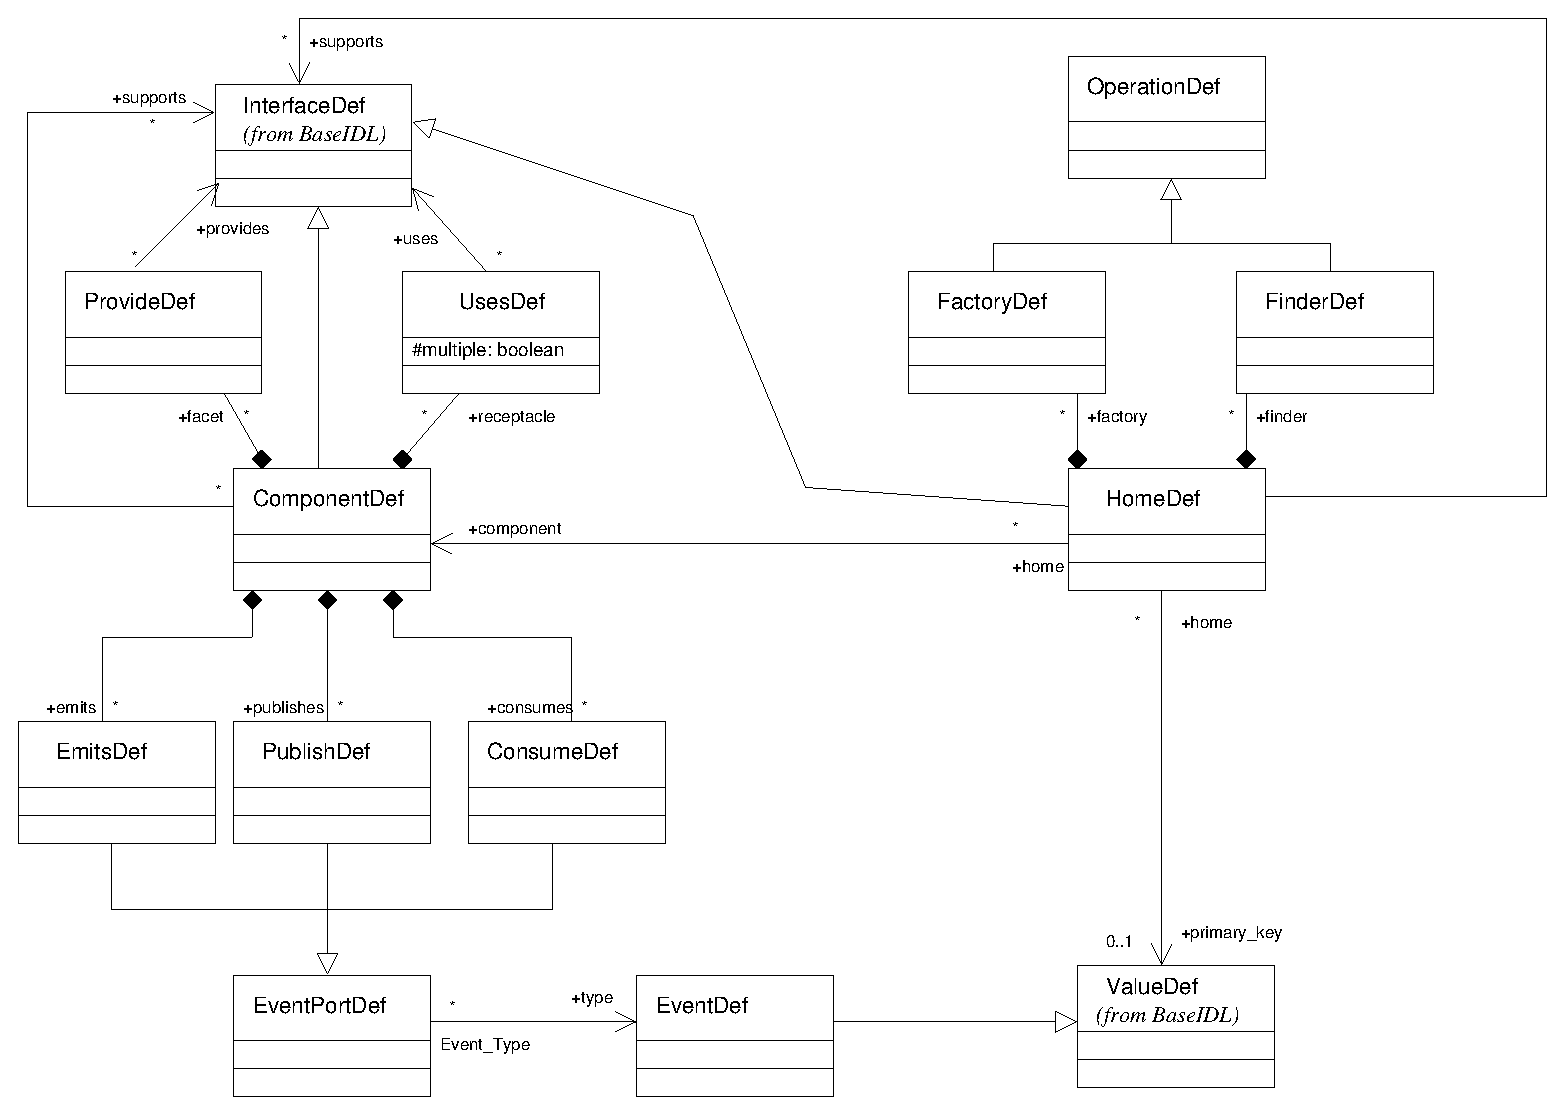
\includegraphics[width=\textwidth]{figures/fig-ccm-model.eps}
    \caption{Corba Component Model (fragment)}
    \label{fig-ccm-model}
\end{figure}

\paragraph{Le mod\`ele abstrait de composants}

Ce mod\`ele est pour l'essentiel la d\'efinition du langage \textsf{IDL3}, un
sur-ensemble du langage de description d'interface de \textsf{CORBA} qui ajoute
un certain nombre de mots cl\'es  permettant de d\'efinir la
structure logique des composant. Un composant est ainsi d\'efini
comme un ensemble d'interfaces fournies et requises, et
d'\'ev\'enements consomm\'es et produits, plus \'eventuellement
des attributs repr\'esentant les
propri\'et\'es configurables du composant. 

\`A chaque composant est
associ\'e une \emph{fabrique} de composants ou \emph{home} qui
est une interface d\'ecrivant les modalit\'es de cr\'eation et,
pour le cas des composants de type entit\'es, de recherche
d'instances de composants.
 Ces d\'eclarations sont projet\'ees en \textsf{IDL2} sous la forme 
d'interfaces \textsf{CORBA} pour pouvoir \^etre accessibles au
travers de l'\textsf{ORB}.
La figure \ref{fig-ccm-model} est un diagramme \textsf{UML}
repr\'esentant les \'el\'ements principaux du \textsf{CCM}.

 \paragraph{Le mod\`ele de programmation}

Il comprend la d\'efinition du langage \textsf{CIDL} ---~\emph{Component Implementation
Definition Language}~---, permettant de d\'efinir
l'implantation d'un composant, et de la plate-forme d'ex\'ecution des
composants (les \emph{containers}). Quatre types de composants sont
d\'efinis : 
\begin{itemize}
\item les composants \textbf{service} ne maintiennent aucun \'etat entre 
  deux appels de m\'ethodes et ne poss\`edent pas d'identit\'e
  propre. Ils sont l'\'equivalent des \emph{EJB Session} sans \'etat ;
\item les composants  \textbf{session} maintiennent un \'etat pour la
  dur\'ee d'une \emph{conversation} avec un client, c'est \`a dire une
  succession d'invocations de m\'ethodes. Lorsque la session est
  termin\'ee --- le plus souvent sur d\'ecision du client, le composant
  perd son identit\'e. Ils sont l'\'equivalent des \emph{EJB Session} avec
  \'etat ;
\item les composants \textbf{processus} persistent entre deux
  invocations mais n'ont pas d'identit\'e. Ils n'ont pas
  r\'eellement d'\'equivalent sur \textsf{J2EE} ;
\item les composants \textbf{entit\'e}, enfin, qui ont un \'etat
  persistant et qui de plus poss\`edent une identit\'e propre au travers
  d'une cl\'e primaire. 
\end{itemize}

\`A chaque type de composant est associ\'e un type de \emph{container} qui 
se charge de la gestion des aspects non fonctionnels ---~persistance,
contexte transactionnel, s\'ecurit\'e, cycle de
vie~--- du composant et du routage des invocations effectu\'ees par les
clients. Les interfaces entre composants et containers sont g\'en\'er\'ees
automatiquement lors de la phase de compilation de la description \textsf{CIDL}. 
Un composant peut \^etre r\'ealis\'e par plusieurs objets au sens
\textsf{CORBA}, les \emph{ex\'ecuteurs}, qui chacun aura la charge d'une partie des
interfaces du composant, \`a charge pour le conteneur d'orchestrer la
cr\'eation des diff\'erentes instances d'objet et leur assemblage.

\paragraph{Le mod\`ele de d\'eploiement}

Le d\'eploiement d'un ou plusieurs composants est d\'ecrit par un
fichier \textsf{XML} qui d\'efinit la mani\`ere d'utiliser un composant 
ou un ensemble de composants en terme d'architecture logicielle et 
de contraintes syst\`emes. Ce \emph{descripteur} est  associ\'e au code du composant  dans un
fichier de d\'eploiement ---~une archive \texttt{.jar}, par exemple~--- qui 
est alors utilisable pour le d\'eveloppement d'une application
compl\`ete. 
Le logiciel de
d\'eploiement utilise ces informations pour dialoguer avec des
serveurs d'assemblage et d'installation afin de mettre en \oe uvre
les composants.

\paragraph{Critiques}

Le \textsf{CCM} reprend dans son mod\`ele abstrait les concepts
principaux des \textsf{ADL} : composants \`a  multiples interfaces,
connecteurs, fabriques de composants. Comme pour les autres
plateformes, le conteneur est l'\'el\'ement cl\'e qui isole le
composant des d\'etails des services techniques. Cette plateforme est
\`a notre avis la plus proche d'une architecture \`a base de
composants et nous nous en sommes d'ailleurs fortement inspir\'es
pour d\'efinir notre mod\`ele de composant (voir chapitre
\ref{chap-fidl}). La r\'ealisation concr\`ete de logiciels bas\'es
sur le \textsf{CCM} reste encore une t\^ache ardue, probablement par
le fait du manque d'outils permettant de s'abstraire des contingences
de l'\textsf{ORB}.

\subsection{Containers de composants}

Les  principaux intergiciels orient\'es composants que nous avons
d\'ecrits succintement ci-dessus sont des plateformes compl\`etes,
complexes et globalement difficiles \`a ma\^{\i}triser de par l'ampleur
des domaines qu'elles essayent de recouvrir. La principale
difficult\'e que l'on rencontre dans la mise en \oe uvre concr\`ete
de ces plateformes est la
quasi-impossibilit\'e dans laquelle se trouvent le concepteur et le
d\'eveloppeur de  s'abstraire des contraintes techniques induites par
les supports d'ex\'ecution et les outils. 

Dans le cas de \textsf{CORBA/CCM},
le d\'eveloppeur se trouve confront\'e \`a un mod\`ele
satisfaisant, suffisamment riche et conceptuellement clair, mais dont
les b\'en\'efices en termes de conception se trouvent quasiment
an\'eantis par la difficult\'e de mise en \oe uvre technique,
quelles que soient les plateformes --- j'ai eu l'occasion
d'exp\'erimenter les plateformes \textsf{OpenCCM} et \textsf{Mico/CCM}. Dans le cas de
\textsf{J2EE}, le probl\`eme de la complexit\'e technique reste entier encore
qu'un peu all\'eg\'e par rapport \`a CORBA, mais par contre le
mod\`ele de composants n'est pas satisfaisant et trop pauvre pour
supporter r\'eellement une conception orient\'ee composants. Enfin,
\`a l'exception de \textsf{.Net}, aucune de ces plateformes ne
supporte la notion pourtant essentielle de \emph{composite}.

R\'ecemment sont apparus un certain nombre de \emph{frameworks} 
dont l'objectif, plus ou moins inspir\'e par les travaux sur
l'\emph{Ing\'enierie Dirig\'ee par les Mod\`eles} ---
\emph{Model Driven Engineering} --- et les \textsf{ADL}, est de permettre
d'une part de construire r\'eellement l'application comme un
assemblage potentiellement hi\'erarchique de composants aux
d\'ependances explicites, d'autre part de ne faire payer aux
d\'eveloppeurs que ce qu'ils utilisent effectivement de
l'infrastructure technique. 

\subsubsection{Spring, Kilim \& PicoContainer}

Ces trois \emph{conteneurs de composants}, r\'ealis\'es initialement en
\textsf{Java} mais depuis partiellement port\'es sur \textsf{.Net}, partagent une m\^eme approche du probl\`eme qui peut
se r\'esumer par la mise en \oe uvre de la notion du \emph{design
  pattern} \og \emph{injection
  de d\'ependances}\fg , bien qu'ils soient tr\`es diff\'erents dans leurs
ambitions. La notion d'\emph{injection de d\'ependances} est un
terme invent\'e par Martin Fowler pour d\'ecrire un patron
de conception orient\'e-objet dans lequel les d\'ependances des
objets entre eux sont remplac\'ees par des d\'ependances vers des
abstractions, c'est \`a dire en \textsf{Java} des interfaces.


 Le plus l\'eger des trois, \textsf{Picocontainer} se veut
un framework extr\^emement simple permettant de 
construire des applications con\c{c}ues comme des assemblages de
composants \`a partir d'objets standards en \textsf{Java}
(POJO). Il offre diff\'erentes implantations de conteneurs et une API
minimaliste permettant d'assembler dynamiquement des instances
d'objets, les \emph{composants}, par d\'ecouverte de leurs
d\'ependances et de leurs interfaces, d\'ecouverte rendue possible
par l'utilisation des capacit\'es r\'eflexives des langages
d'implantation.

\textsf{Kilim} est bas\'e sur le m\^eme principe mais ajoute la
possibilit\'e de d\'ecrire les assemblages et la configuration des
composants dans un descripteur externe qui sera charg\'e par le
moteur au lancement  de l'application.

\textsf{Spring} enfin, est le plus complet  de ces frameworks et se
veut une infrastructure transversale destin\'ee \`a faciliter le
d\'eveloppement d'applications \textsf{J2EE} en implantant un mod\`ele de
composants. Comme pour les pr\'ec\'edents projets
cit\'es, Spring utilise l'\emph{injection de d\'ependances} pour
r\'ealiser au moment de son d\'eploiement des assemblages de
composants, composant \'etant ici comme pr\'ec\'edemment synonyme
d'objet.

\subsubsection{Fractal}
\label{sec:fractal}
Fractal est un mod\`ele de composant d\'ecoupl\'e de toute
implantation concr\`ete et qui pr\'esente un certain nombre de
caract\'eristiques originales. Le mod\`ele de base d\'etaill\'e
dans \cite{fractal-spec} se pr\'esente comme un ensemble
d'interfaces  d\'efinissant les exigences 
que doit remplir toute impl\'ementation du mod\`ele. Un composant
est ici compos\'e d'un \emph{contr\^oleur} ou  \emph{membrane} et de
sous-composants, \'eventuellement \emph{partag\'es} entre diff\'erents
composites. Les composants interagissent au moyen d'\emph{interfaces}
qui peuvent \^etre \emph{externes} ou \emph{internes} --- accessibles
uniquement aux composants encapsul\'es. Des interfaces de contr\^ole
g\'en\'eriques sont d\'efinies permettant d'offrir des
m\'ecanismes d'introspection, de liaison dynamique et de gestion du
cycle de vie.

Les caract\'eristiques les plus originales du mod\`ele sont : 
\begin{itemize}
  \item la s\'eparation d'un composant entre son corps et sa
    \emph{membrane} qui permet
    de d\'efinir de v\'eritables comportements pour l'interface d'un
    composant ou d'une architecture de composants, sans pr\'ejuger de
    son implantation. On peut ainsi d\'efinir des \emph{membranes}
    g\'erant la s\'ecurit\'e, des membranes filtrant ou retraitant
    les messages, des membranes poss\'edant tel ou tel
    service ;
  \item la prise en compte explicite des \emph{composites} comme des
    composants \`a part enti\`ere. Un composant peut
    \'eventuellement offrir des interfaces d'administration sur sa
    structure, ou la laisser totalement opaque ;
  \item le \emph{partage} des composants entre diff\'erents assemblages.
\end{itemize}

Ce mod\`ele poss\`ede une implantation de r\'ef\'erence en
\textsf{Java} d\'enomm\'ee \textsf{Julia} et a servi aussi \`a la
r\'ealisation de composants permettant de construire une sorte d'\emph{OS
en kit}. Il est au centre de plusieurs travaux de recherche et
poss\`ede une communaut\'e de d\'eveloppement relativement
active au travers du consortium \textsf{ObjectWeb}.

Le mod\`ele \textsf{Fractal} est int\'eressant ne serait-ce que par sa
relative \'economie de moyens lorsqu'on le compare aux plateformes
classiques. \`A notre avis, seule toutefois la d\'efinition explicite
de composites est r\'eellement un atout : la notion de membrane,
intellectuellement s\'eduisante n'est qu'une reformulation des
connecteurs et n'est pas un concept primitif d'architecture car il est
toujours possible de la remplacer par des familles de composants
sp\'ecifiques. Le partage de composants, quant \`a lui, pose des
probl\`emes de formalisation des d\'ependances, de
contractualisation des interactions et d'encapsulation des assemblages.

\section{Langages de Description \& de Conception d'Architecture}
\label{sec:lang-de-descr}

La pr\'ec\'edente section \'etait d\'edi\'ee aux plateformes et
outils pour la manipulation concr\`ete de composants. Nous remontons
d'un cran dans l'abstraction en examinant quelques propositions
permettant de concevoir des architectures de composants. La
premi\`ere partie est consacr\'ee aux langages de conceptions
g\'en\'eralistes. Leur caract\'eristique commune est de couvrir un
spectre tr\`es large de situations et par cons\'equent d'avoir une
s\'emantique relativement faible pour la mod\'elisation du
comportement des composants. La deuxi\`eme partie s'int\'eresse plus
particuli\`erement aux \textsf{ADL} sp\'ecialement con\c{c}us pour
repr\'esenter des architectures et des composants.

\subsection{UML}
\label{sec:uml}
\textsf{UML} est aujourd'hui l'outil de base pour la conception et
l'analyse des applications, gr\^ace \`a la simplicit\'e de ses
concepts de base et \`a la profusion d'outils existants pour
manipuler des mod\`eles. Le point fort d'\textsf{UML}, sa versatilit\'e, est  aussi son point faible : l'actuelle norme 2.0 est encore
en phase d'adoption au sein du consortium \textsf{OMG} et
l'int\'egration de la multitude de diagrammes disponibles ainsi que
le flou entourant leur s\'emantique rendent l'implantation
d'un processus r\'eellement dirig\'e par les mod\`eles encore
tr\`es difficile.

La notion de \emph{composant} est pr\'esente dans les versions
pr\'ec\'edentes du langage uniquement comme repr\'esentation d'une
entit\'e concr\`ete du syst\`eme d\'eploy\'ee sur une
architecture physique. Cette notion a \'et\'e \'etendue \`a celle
d'unit\'e de composition architecturale avec l'introduction des
\emph{diagrammes de composants}. Ces diagrammes, dont nous donnons un exemple tir\'e de la
sp\'ecification\cite{uml20-comp} dans la figure
\ref{fig-uml20-comp-sample}, permettent d\'esormais de repr\'esenter
explicitement des architectures de composants.

\begin{figure}[htbp]
    \centering
    \includegraphics[width=.9\textwidth]{figures/fig-uml20-comp-sample.eps}
    \caption{Exemple de diagramme de composants UML 2.0}
    \label{fig-uml20-comp-sample}
\end{figure}

De plus, il est d\'esormais possible d'attacher aux ports des
composants des sp\'ecifications de \emph{protocole} sous la forme de
\emph{State Machines} ce qui permet d'utiliser \textsf{UML} comme un \textsf{ADL} \`a
part enti\`ere. 

Ces diagrammes ont le m\'erite d'\^etre simples dans leurs principes
et de ne pas surcharger le langage. Les composants peuvent \^etre
d\'etaill\'es au moyen de la syntaxe \textsf{UML} existante :
diagrammes de classes, diagrammes d'\'etats-transitions. La notion
de connexion reste toutefois confondue avec celle de d\'ependance et
seuls les ports de type synchrone sont pris en compte
explicitement. 

\subsubsection{EDOC}
\label{sec:edoc}
\textsf{EDOC} --- \emph{Enterprise Distribued Object Computing} ---
est  un profil UML, c'est \`a dire une
sp\'ecialisation du langage UML et de son m\'eta-mod\`ele pour
repr\'esenter des concepts sp\'ecifiques \`a un domaine
d'application, une technologie ou un processus. C'est une norme
adopt\'ee par l'\textsf{OMG} en 2001. \textsf{EDOC} est une
alternative int\'eressante car plus compl\`ete aux \emph{diagrammes
  de composants} pour la mod\'elisation d'architectures de
composants. 

Le c\oe ur de \textsf{EDOC} est constitu\'e de l'\emph{Architecture de Collaboration
de Composants}  qui d\'efinit les concepts
d'architecture, d'assemblage, de composants et d'interactions en
termes de mod\`eles \textsf{UML}. L'objectif affich\'e de ce mod\`ele est de
r\'epondre \`a diff\'erents probl\`emes : 
\begin{itemize}
  \item la composition r\'ecursive de composants pour mod\`eliser des
    syst\`emes \`a diff\'erents niveoux d'abstractions ;
  \item  la
    \emph{tra\c{c}abilit\'e} de l'\'evolution des mod\`eles et des
    implantations, l'automatisation du processus du d\'eveloppement
    au travers d'une d\'emarche \textsf{MDA} ;
  \item  le couplage faible
    entre \'el\'ements d'un syst\`eme pour promouvoir la
    r\'eutilisation et l'\'evolution concurrente de diff\'erentes
    parties d'un syst\`eme ;
  \item  l'ind\'ependance envers les technologies ;
    \item et enfin l'\'emergence d'un march\'e des composants m\'etiers.
\end{itemize}
La figure \ref{fig-edoc-comp-sample} repr\'esente un
composite dans la notation \textsf{EDOC} ou \emph{processus
communautaire}  mod\'elisant un syst\`eme
d'achat-vente. Ce sch\'ema d\'etaille diff\'erents types de ports et
en particulier des \emph{multiports} ou protocoles.

\begin{figure}[htbp]
    \centering
    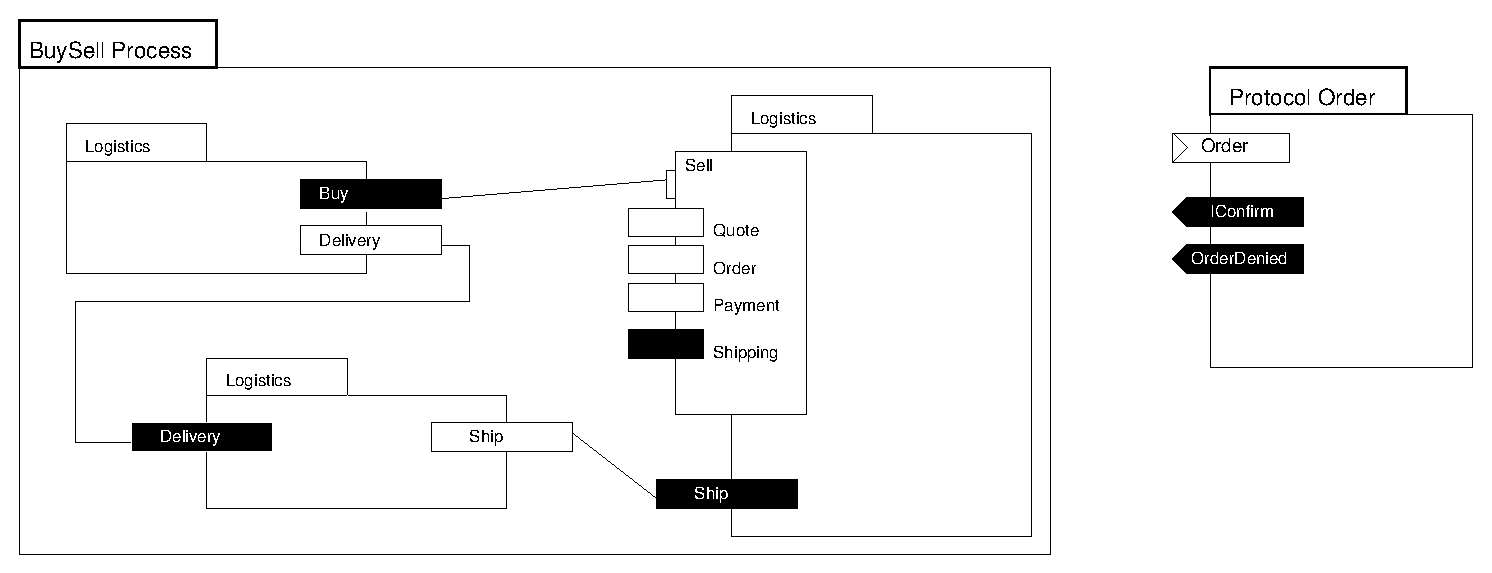
\includegraphics[width=.9\textwidth]{figures/fig-edoc-comp-sample.eps}
    \caption{Exemple de sch\'ema de composite EDOC}
    \label{fig-edoc-comp-sample}
\end{figure}

Les ports d'un composant sont :
\begin{itemize}
  \item soit des \'emetteurs ou r\'ecepteurs d'\'ev\'enements
  atomiques ;
\item soit des ports d\'efinissant un \emph{protocole d'interaction}
  dont le composant est l'initiateur ou le r\'epondeur,
  d\'ecrit au moyen d'un diagramme d'activit\'e ---une
  \emph{chor\'egraphie} dans la terminologie officielle --- et
  subdivis\'es eux-m\^emes en ports de granularit\'e plus fine. 
\end{itemize}
Si le mod\`ele de communication est au niveau le plus fin un
mod\`ele \emph{asynchrone} bas\'e sur des flots d'\'ev\'enements,
les protocoles permettent d'imbriquer des  s\'equences
d'\'ev\'enements et de protocoles pour constituer une
\emph{transaction} plus globale. Une \emph{op\'eration} au sens UML
du terme est vue comme un ensemble de flots li\'es par une
s\'emantique d'appel-retour.

Ce mod\`ele de base est \'etendu en un \emph{mod\`ele de processus
  m\'etiers} --- \emph{business process model} --- qui permet
de d\'efinir des 
processus concurrents communiquant par flots de donn\'ees en tant que composants.

Comme \`a l'accoutum\'ee, le document de normalisation est  tr\'es
pr\'ecis et d\'etaill\'e,  d\'ecrivant chacun des \'el\'ements
du profil, la notation associ\'ee, les contraintes stucturelles et la
s\'emantique de chacune des constructions. Cette proposition nous a
paru tr\`es int\'eressante, ne serait-ce que par ses objectifs qui
recouvrent une partie de nos pr\'eoccupations. Il
manque toutefois une formalisation explicite et compacte de la
s\'emantique des syst\`emes et architectures consid\'er\'es.

\subsubsection{AADL}

Le \emph{langage de conception et d'analyse d'architecture}\cite{aadl-overview} ---
\emph{Architecture Analysis \& Design Language} en anglais --- est une
proposition de standardisation de l'ing\'enierie dirig\'ee par les
mod\`eles et l'architecture pour les syst\`emes embarqu\'es
critiques d\'evelopp\'ee par la \emph{Society for  Automotive
  Engineers}. Cette proposition s'appuie sur les travaux de
normalisation de l'OMG dans le cadre de \textsf{UML 2.0} et les
travaux ant\'erieurs sur des outils de m\'eta-mod\'elisation tels
que \textsf{MetaH}.

\textsf{AADL} se pr\'esente essentiellement comme un socle commun de
concepts sur lequel pourront s'appuyer des outils de d\'eveloppement
et d'\'echange de mod\`eles, cibl\'e en direction de la
mod\'elisation de syst\`emes embarqu\'es. Il prend en compte 
la mod\`elisation des plateformes d'ex\'ecution au travers de
diff\'erents composants d'abstraction --- processeur, bus,
p\'eriph\'erique, m\'emoire ; et de composants logiciels parmi
lesquels on distingue des composants actifs --- \emph{threads}  et
processus --- et des composants passifs --- paquetages et donn\'ees.
\`A chaque composant peuvent \^etre attach\'ees des
\emph{propri\'et\'es} pr\'ed\'efinies ou sp\'ecifiques, et des
contraintes sur ces propri\'et\'es qui permettent de mod\'eliser et
v\'erifier des exigences \emph{temps-r\'eels}.

Les composants interagissent au travers de ports qui classiquement
isolent un composant des autres \'el\'ements du syst\`eme, ports
qui supportent trois modes de communication : le flot de donn\'ees
typ\'e avec une s\'emantique d'interruption --- au sens
d'interruption dans les syst\`emes d'exploitation --- ou de files, l'appel
de proc\'edure et le partage de variables.

Des outils existent, en particulier pour la plateforme
\textsf{Eclipse}, mais pour l'instant ils se limitent \`a
permettre la manipulation de mod\`eles au travers de diverses
interfaces  et des
v\'erifications de consistance interne des mod\`eles. \textsf{AADL} est
essentiellement une norme d'\'echange de mod\`eles, dont les forces
affich\'ees, la capacit\'e \`a int\'egrer des contraintes sp\'ecifiques aux
domaines et les points d'extension, nous paraissent \^etre
plut\^ot des inconv\'enients. Ce langage est en quelque sorte le
pendant pour le temps-r\'eel de \textsf{EDOC}. 

\subsection{ADL}

\cite{survey-long} propose une taxonomie des
principaux \textsf{ADL} selon plusieurs axes. Cette \'etude assez
large identifie les concepts du domaine et la mani\`ere dont chaque
langage les d\'efinit et 
permet de les manipuler. Nous avons choisi de nous int\'eresser dans les paragraphes qui suivent
\`a deux \textsf{ADL} non pr\'esent\'es dans cette \'etude et qui nous ont parus
pr\'esenter des caract\'eristiques proches de nos pr\'eoccupations
: \textsf{SOFA} et \textsf{ArchJava}. Toutefois, nous introduisons la
discussion avec une analyse de deux \textsf{ADL} \og classiques\fg
\textsf{Wright} et \textsf{Rapide}, parmi les premiers
\textsf{ADL} \`a supporter une s\'emantique formelle. 

\subsubsection{Wright \& Rapide}
\label{sec:wright}

\textsf{Wright}\cite{archcon} est \`a l'origine avec
\textsf{UniCon}\cite{shaw-abstract-archi}  de l'introduction de
\emph{connecteurs} formellement sp\'ecifi\'es entre composants,
c'est \`a dire de la d\'efinition de protocoles de communication
entre composants d'un syst\`eme. Les composants et connecteurs sont
sp\'ecifi\'es par des expressions \textsf{CSP}\cite{hoare-csp} avec la
s\'emantique en termes de traces et de refus de ce langage. Un
connecteur est vu comme l'ex\'ecution en parall\`ele de plusieurs
processus d\'ecrivant les \emph{r\^oles} dans lesquelles le
connecteur peut-\^etre utilis\'e et un processus \emph{colle}
d\'ecrivant les interactions entre r\^oles. Un composant est
d\'efini aussi par des expressions \textsf{CSP} d\'ecrivant ses diff\'erents
\emph{ports} et son comportement. 

La compatibilit\'e
entre r\^oles --- d'un connecteur --- et port --- d'un composant ---
et donc la correction d'une architecture donn\'ee, est assur\'ee par
la v\'erification d'une relation de \emph{raffinement} \'etendue
entre processus. Plus pr\'ecis\`ement, un port est compatible avec
un r\^ole si l'intersection des traces du port et des traces
d\'eterministes du r\^ole est un raffinement de l'ensemble de traces
du r\^ole. Une propri\'et\'e importante que l'on peut v\'erifier
est l'absence d'interblocage dans une configuration architecturale
donn\'ee. 

La motivation principale de \textsf{Wright} pour la
mod\'elisation explicite des connecteurs est d'exprimer
un nombre vari\'e de politique de communication. Elle
permet d'appliquer le formalisme sur une plus large gamme de syst\`emes en
d\'ecouplant la description des interactions de la description des
fonctionnalit\'es des composants. Les premi\`eres sont  
consid\'er\'ees g\'en\'eralement comme peu variables pour une
famille de syst\`emes donn\'ee  tandis que les seconds sont \emph{a
contrario} tr\'es variables. On notera, et c'est un point
aussi soulign\'e par les auteurs que l'on peut parvenir au m\^eme
r\'esultat en utilisant uniquement des composants et une seule
modalit\'e de communication.

Rapide \cite{rapide} est un syst\`eme complet de sp\'ecification et
de d\'eveloppement de syst\`emes distribu\'es orient\'es objets
guid\'e par l'architecture. Les composants sont des objets
concurrents, hi\'erarchiques, typ\'es par interfaces et implant\'es
par des modules. Ils communiquent par des connexions explicites en
\'emettant des \emph{actions} et invoquant des
\emph{fonctions}. L'ensemble des \'ev\'enements d'un syst\`eme
forme un ordre partiel d'\'ev\'enements qui constitue la base de la
s\'emantique d'ex\'ecution. 

Les  \emph{interfaces}  d\'efinissent des signatures d'actions et de
fonctions requises et fournies et \'eventuellement un \emph{contrat}
sous la forme de contraintes comportementales, sur le contenu des
messages \'echang\'es au travers de l'interface, et sur la
causalit\'e entre \'ev\'enements re\c{c}us et \'emis par
l'interface. Une \emph{architecture} d\'efinit l'implantation
d'une interface en termes d'interfaces imbriqu\'ees et de leurs connexions. Les \emph{connexions}
d\'efinissent des relations de causalit\'e entre ordre partiels
d'\'ev\'enements soit entre \'ev\'enements externes, soit entre
\'ev\'enements externes et internes. La notion de service permet de
regrouper un ensemble d'\'ev\'enements dans un type et de connecter directement
des services compl\'ementaires. Enfin, la notion de \emph{mapping}
permet de d\'efinir des transformations d'un ensemble
d'\'ev\'enements dans un autre, offrant ainsi la possibilit\'e de
d\'ecrire des relations entre diff\'erents niveaux d'abstractions.
Les propri\'et\'es que l'on peut v\'erifier sont nombreuses : la conformit\'e d'une architecture par rapport \`a son
interface, d'une implantation par rapport \`a son architecture, des
propri\'et\'es sur les s\'equences d'\'ev\'enements, ...

\subsubsection{ArchJava}

ArchJava\cite{aldrich-archjava,aldrich-archjava-reasoning} est une
extension au langage \textsf{Java} similaire \`a un ADL permettant d'int\'egrer des
contraintes architecturales dans du code source. Les extensions au
langage permettent de v\'erifier des propri\'et\'es
d'\emph{int\'egrit\'e des communications} : les objets communiquent entre
eux uniquement par les ports sp\'ecifi\'es. Ces propri\'et\'es
sont v\'erifi\'ees \`a la compilation par une extension du
syst\`eme de type de Java int\'egrant les notions de ports, de
composants et de composites. On v\'erifie ainsi que des composants ne
peuvent communiquer qu'avec des membres d'un m\^eme composite, des
sous-composants ou le composant englobant. 

Un \emph{composant} est une instance d'une classe \texttt{component}
contenant des d\'efinitions de \emph{ports}. Un port est un ensemble
de m\'ethodes qui peuvent \^etre \emph{fournies}, \emph{requises} ou
\emph{diffus\'ees} (\emph{broadcast}). Les m\'ethodes fournies doivent
\^etre implant\'ees par le composant, les m\'ethodes requises
\'etant fournies par l'autre extremit\'e de la connexion. 

Un port peut \^etre d\'efini au moyen d'un type \emph{interface de
  port} contenant uniquement des signatures de m\'ethodes
  fournies, offrant ainsi la possibilit\'e de d\'efinir
  dynamiquement le composant implantant r\'eellement le port. 

Un \emph{composite} est un composant contenant d'autres composants et qui
d\'ecrit des connexions ou des sch\'emas de connexion autoris\'es
entre ses sous-composants, et \'eventuellement avec ses propres
ports. Un composite dispose de la capacit\'e d'invoquer directement
les m\'ethodes de ses sous-composants, l'inverse n'\'etant pas vrai.

Dans  \cite{aldrich-archjava-reasoning}, un mod\`ele formel du
langage ArchJava est d\'efini essentiellement au travers d'un syst\`eme de types
et d'une s\'emantique op\'erationnelle. Ce mod\`ele est
bas\'e sur FeatherweightJava \cite{featherweightjava}, une
formalisation du langage \textsf{Java} usuel. On
v\'erifie \`a l'aide de ce mod\`ele que l'int\'egrit\'e des communications est bien maintenue
par le typage et certaines instructions \`a l'ex\'ecution
(v\'erification du transtypage) :
\begin{itemize}
  \item un composant $C$ ne peut appeler directement des m\'ethodes
    d'un composant $C'$ que si $C=C'$ ou si $C'$ est un sous-composant
    de $C$ ;
  \item dans tous les autres cas, la communication entre composants se
    fait au travers de leurs ports.
\end{itemize}

Le principal int\'er\^et du mod\`ele \textsf{ArchJava} est sa
proximit\'e avec le langage \textsf{Java} ce qui permet d'int\'egrer
facilement des concepts architecturaux dans les d\'eveloppements, la
correction \'etant assur\'ee par le syst\`eme de types. C'est aussi
son principal inconv\'enient qui rend ce mod\`ele trop li\'e \`a
une impl\'ementation pr\'ecise --- en l'occurence un langage et une
plateforme d'ex\'ecution --- et surtout qui induit un glissement des
probl\'ematiques architecturales de la conception vers la
r\'ealisation ce qui n'est pas l'objectif souhait\'e. De plus, les
concepts de composants se t\'elescopent avec les concepts objets
usuels du langage ce qui peut rendre l'utilisation de ce syst\`eme
\`a grande \'echelle tr\`es d\'elicate. 

\subsubsection{SOFA}

Le mod\`ele \emph{SOFA} --- pour \emph{Software Appliances} --- est
d\'etaill\'e pour l'essentiel dans \cite{plasil-sofa} et fait
partie d'un projet plus large d'une plateforme de conception de
composants, par ailleurs int\'egr\'e dans le consortium
\emph{Objectweb}.  L'objectif du mod\`ele, qui emprunte la majeure
partie de ses concepts aux \textsf{ADL}, est de permettre la \emph{validation statique}
de syst\`emes de composants hi\'erarchiques, la validit\'e du raffinement
d'architecture dans l'\'etape de conception, et la v\'erification
dynamique au travers de l'embarquement d'assertions d\'eriv\'ees du
langage de sp\'ecification \`a l'ex\'ecution.

Le concept de base de \textsf{SOFA} est la notion de \emph{protocole} d\'efinissant un
langage sur un
alphabet compos\'e de messages de type requ\^ete-r\'eponse. Ce
langage est rationnel ou approch\'e par un rationnel. Un
protocole peut \^etre attach\'e \`a une \emph{connexion}, c'est
\`a dire un lien bidirectionnel entre deux entit\'es. Ou il
peut \^etre attach\'e  \`a un
\emph{agent}, c'est \`a dire une entit\'e utilisant une ou plusieurs
connexions pour communiquer avec son environnemnt. L'alphabet d'un
protocole est partitionn\'e entre un ensemble de messages
fournis  et un ensemble de messages requis.

Un \emph{cadre}  d\'efinit un ensemble
d'interfaces fournies et requises, une interface \'etant une
collection de m\'ethodes, et un protocole sur les alphabets induits
par ces interfaces. Une \emph{architecture} est la r\'ealisation d'un
cadre par un ensemble d'autres cadres et la d\'efinition de
connexions entre ceux-ci, autrement dit une structure sens\'ee
implanter le cadre. Ces deux \'el\'ements peuvent se combiner de
mani\`ere hi\'erarchique jusqu'\`a atteindre les composants
primitifs par d\'efinition indivisible.

La principale propri\'et\'e que l'on peut d\'efinir et v\'erifier
sur les diff\'erentes entit\'es composant un syst\`eme est la
notion de \emph{substituabilit\'e de protocole} qui permet de
s'assurer de la compatibilit\'e d'une architecture avec une frame et
des deux parties prenantes dans une connexion.  Cette propri\'et\'e
s'\'enonce informellent comme $A$ est substituable \`a $B$ si :
\begin{enumerate}
  \item  $A$ fournit au moins tous les services fournis par $B$ :
  \item et $A$ ne requiert pas plus de son environnement que n'en aurait
  exig\'e $B$ \emph{dans les m\^emes conditions}.
\end{enumerate}

\section{Sp\'ecification formelles \& composants}

Cette derni\`ere section est consacr\'ee \`a des mod\`eles tr\`es
th\'eoriques prenant en compte des probl\'ematiques de composition et de
connexions de composants. 

\subsection{\pc et Alg\`ebres de processus}

Le \pc\cite{calcmp1,calcmp2} est une alg\`ebre de processus
destin\'ee \`a mod\'eliser et
\'etudier les propri\'et\'es des syst\`emes distribu\'es. Ce
formalisme se distingue de ses pr\'ecurseurs et de ses successeurs par une
remarquable \'economie de moyens syntaxiques et une expressivit\'e
non moins remarquable. 
L'\'el\'egance et l'expressivit\'e  du
langage proviennent de l'uniformit\'e de traitement offerte par la
notion de \emph{noms}, un terme tr\`es abstrait qui est \`a la fois une
variable, un identifiant de canal de communication et une donn\'ee
que l'on peut \'echanger. 

La notion d'\'equivalence comportementale est captur\'ee par le
concept de \emph{bisimulation}, relation fondamentale entre les termes
du \pc et que nous retrouverons dans
le chapitre \ref{chap-etatarttest} consacr\'e au test de composants. Le principal
inconv\'enient du \pc est aussi son principal avantage : sa
\emph{puissance}. Cette puissance  induit \emph{de facto}
l'ind\'ecidabilit\'e de la plupart des propri\'et\'es
int\'eressantes dans le cas de la version g\'en\'erale du langage
 et en particulier de
l'\'equivalence comportementale des termes, donc de la relation de
bisimulation. La sobri\'et\'e de la syntaxe et de la s\'emantique
rendent inutilisable le \pc autrement que comme objet de r\'eflexion
th\'eorique, et c'est pourquoi de nombreux travaux ont cherch\'e
\`a accro\^{\i}tre son \og \emph{utilisabilit\'e}\fg, par exemple au
travers de calculs polyadiques, de l'introduction de types primitifs
et d'un syst\`eme de types sur les termes.

\subsubsection{Piccola}
\textsf{Piccola} est un langage de composition d\'evelopp\'e par le
\emph{Software Composition Group} de
Berne\cite{piccola,formallangcomp,compsoftres}. Bien qu'il ne
s'agisse pas \`a proprement parler d'une plate-forme de composants,
cette approche nous semble int\'eressante car elle met l'accent sur la
notion de connecteurs, r\'eifi\'es sous la forme de scripts
\textsf{Piccola}. Ces scripts permettent \`a des composants \'ecrits
simplement en \textsf{Java} de s'\'echanger des donn\'ees structur\'ees
---~appel\'ees \emph{forms}~--- en s'abstrayant de l'architecture
mat\'erielle et logicielle de l'application. La s\'emantique du
langage est bas\'ee sur une version du \pc, le \pc asynchrone
polyadique dans lequel les op\'erations de communication peuvent
mettre en \oe uvre des n-uplets de noms et sont r\'ealis\'ees  de
mani\`ere asynchrone. Il ne semble pas
toutefois que ces d\'eveloppements s'int\'eressent \`a la v\'erification et \`a la validation de
programmes autrement qu'au moyen d'un syst\`eme de types\cite{regtypes}. 

\subsubsection{Darwin}

\textsf{Darwin}\cite{darwin} est  un \textsf{ADL} qui
permet de d\'efinir des architectures de composants inter-connect\'es
et hi\'erarchiquement structur\'es, et dans lequel la s\'emantique
des op\'erations de connexion est d\'efinie au moyen de termes du
\pc polyadique synchrone. L'id\'ee centrale consiste \`a attacher
\`a chaque port de service fourni et requis un terme du \pc et, \`a
partir d'une configuration donn\'ee, de v\'erifier par application
des r\`egles de r\'eduction du calcul que la configuration est
correcte, c'est \`a dire que chaque port requis se trouve connect\'e
au bon port fourni. Ce principe de base est \'etendu au probl\`eme
de la cr\'eation de nouvelles instances de composants, cr\'eation
qui est exprim\'ee aussi comme un terme du \pc et dont la
s\'emantique permet de v\'erifier \`a la
conception  et \`a l'ex\'ecution sa viabilit\'e en fonction d'un contexte. Notons que ce
langage ne s'int\'eresse pas au fonctionnement des
composants ni \`a la sp\'ecification de leurs services mais
uniquement \`a la validation d'une structure donn\'ee. 

\subsubsection{CORBA \& \pc}

Les travaux de \cite{refinepi,picorba} utilisent le
\pc pour sp\'ecifier le comportement d'interfaces CORBA et
\cite{canal-compat-arch} en d\'etaillent les aspects formels. Le
comportement d'interfaces --- roles --- et de composants d'un
syst\`eme est sp\'ecifi\'e sous la forme d'agents du \pc, et une
relation de \emph{compatibilit\'e} entre agents est propos\'ee
permettant de v\'erifier la conformit\'e de deux interfaces entre
elles dans l'optique par exemple d'adapter  le comportement de l'une
\`a l'autre et de pouvoir d\'eriver automatiquement des
\emph{adaptateurs} et connecteurs poss\'edant certaines
propri\'et\'es et compatibles avec une architecture donn\'ee.
Une \emph{relation de compatibilit\'e} permet de prouver que la composition de deux composants
au travers de leurs interfaces est correcte si les \emph{connexions}
entre interfaces sont compatibles, une propri\'et\'e importante que
nous \'etudierons dans le contexte qui est le notre au chapitre
\ref{cha:composition}. Enfin, une relation d'h\'eritage entre agents
et d'extension de comportement est d\'efinie qui pr\'eserve la
compatibilit\'e des interfaces. 

Dans \cite{bracciali-comp-adapt}, le probl\`eme de l'adaptation
automatique du comportement d'interfaces est \'etudi\'e dans le
cadre pr\'esent\'e ci-dessus. La technique utilis\'ee consiste \`a
construire incr\'ementalement un \emph{agent d'adaptation}, c'est \`a dire un terme du
\pc, \`a partir d'une application --- \emph{mapping} --- entre les
signatures et les contraintes de chacune des interfaces \`a adapter,
de sorte que le nouvel agent compos\'e avec les deux agents initiaux
produise un comportement correct.

Le choix du \pc est ici, comme pour les travaux
pr\'ec\'edemment cit\'es, guid\'e par la capacit\'e de cette
th\'eorie \`a mod\'eliser facilement la mobilit\'e et la dynamique
structurelle des syst\`emes. 
Il n'est bien s\^ur pas le seul formalisme de la famille des
alg\`ebres de processus \`a avoir \'et\'e utilis\'e pour
sp\'ecifier le comportement d'architectures logicielles : l'\textsf{ADL}
\emph{Wright}, par exemple, (voir  section \ref{sec:wright}) utilise
\textsf{CSP} comme outil de sp\'ecification de comportements et le
\emph{kell-calcul} est une variante complexe du calcul des ambients pour
d\'efinir une s\'emantique formelle \`a la plateforme \textsf{Fractal}.
 
\subsubsection{M-Calcul \& Kell-Calcul}

Le \textsf{M-calcul}\cite{M-calcul} est un \emph{calcul de processus} inspir\'e de
pr\'ed\'ecesseurs tels que le \emph{calcul des ambients}, le
\emph{join-calculus}, le \emph{blue calculus}, la \emph{Chemical
  Abstract Machine}. C'est \`a dire qu'il s'int\'eresse non
seulement aux processus, \`a leurs compositions au travers
d'op\'erateurs alg\'ebriques, mais aussi \`a la notion, centrale
pour les mod\`eles \`a composants, d'encapsulation et de
structure. La principale entit\'e de ce calcul est la \emph{cellule}
qui, par analogie avec la cellule biologique, est constitu\'ee d'une
\emph{membrane}  et d'un \emph{plasme}, chacun \'etant d\'ecrit
comme  un processus.

Le point qui distingue le \emph{M-calcul} de ses concurrents est la
mani\`ere dont ont lieu les communications entre cellules. Les
cellules sont organis\'ees de mani\`ere hi\'erarchique \`a partir
d'une racine, le syst\`eme. La membrane agit comme un contr\^oleur
et un filtre sur les messages qui entrent  et sortent du plasme, ce qui
autorise toutes sortes de mod\'elisations de syst\`emes distribu\'es
complexes : firewalls, syst\`emes d'authentification, syst\`emes
tol\'erants aux pannes, r\'esolution dynamique de noms, ... 

Le \emph{kell-calcul}\cite{kell-calculus} est un raffinement du M-calcul dans
lequel ont disparu les concepts distincts de membrane et de plasme au
profit d'une vision plus uniforme de processus imbriqu\'es \emph{\`a la}
calcul des ambients.  La communication est rendue plus abstraite et
plus g\'en\'erale par l'utilisation d'un m\'ecanisme de
filtrage de motifs param\'etrant le
langage, d'o\`u la qualification du kell-calcul comme une famille
de langages. Ce filtrage op\`ere sur la structure des messages
\'echang\'es entre les diff\'erentes cellules ou \emph{kells} 
et peut \^etre arbitrairement complexe. L'objectif de
ce projet est de fournir une s\'emantique formelle, compl\'et\'ee
de l'arsenal usuel : syst\`eme de types, relations d'\'equivalences,
r\'esultats de d\'ecidabilit\'e, pour la plate-forme de composants
\textsf{Fractal} (voir section \ref{sec:fractal}).

\subsection{Composants \& Coalg\`ebres}

Les approches pr\'esent\'ees ci-dessous s'inscrivent dans la
th\'eorie des co-alg\`ebres d\'efinie en termes cat\'egoriques et
dont une synth\`ese est donn\'ee  dans \cite{coalgebra-tutorial}. La
notion de co-alg\`ebre \emph{dualise} la notion d'alg\`ebre et
permet de d\'efinir un cadre pour la sp\'ecification abstraite de
syst\`emes dynamiques au comportement infini, la comparaison par bisimulation et la preuve
par co-induction.

\subsubsection{Abstract Behavior Types \& \textsc{Reo}}

Le mod\`ele de composants propos\'e dans \cite{ABT} est bas\'e sur
la notion de \emph{type abstrait de comportement} d\'efini comme une
relation entre des \emph{flots de donn\'ees temporis\'es}
d'entr\'ee et de sortie. Informellement, les composants
mod\'elis\'es sont suppos\'es \'echanger des messages avec
leur \emph{environnement} au travers d'interfaces soit en entr\'ee,
soit en sortie. Une interface est un flot
de donn\'ee temporis\'e, c'est \`a dire une paire de s\'equences
infinies d'\'el\'ements d'un ensemble quelconque et
de r\'eels strictement croissants. Les
\'ev\'enements sont suppos\'es ordonn\'es, atomiques et
poss\`edent une dur\'ee non nulle. 

Un composant est ainsi un ensemble de flots de donn\'ees temporis\'es,
\'etiquet\'es comme entr\'ee ou sortie, et la relation existant
entre ces flots. Ce mod\`ele permet de donner une s\'emantique au
langage de composition \textsc{Reo} introduit par ailleurs dans
\cite{constraint-automata}.  Ce langage d\'efinit un ensemble de connecteurs
et de composants primitifs composables pour produire des syst\`emes plus larges. 

Un connecteur en \textsc{Reo} est un ensemble de \emph{canaux}
organis\'es en graphe o\`u les n\oe uds sont des regroupements de
points d'attaches de canaux et les arcs  entre deux n\oe uds
contenant les points d'attache du canal. Un canal est un medium de
communication entre deux points d'attache. Cet ensemble minimal de
d\'efinitions est compl\'et\'e par une op\'eration de regroupement
de points d'attache, ou \emph{join}, r\'eunissant plusieurs points
d'attache dans un seul n\oe ud, et une s\'emantique de transmission
des messages dans les n\oe uds qui permet en particulier de
r\'epliquer les messages sur tous les canaux li\'es \`a un point
d'attache.

L'int\'er\^et principal de cette approche est l'accent mis sur la
topologie abstraite des connecteurs et des n\oe uds. Cette structure
et ses op\'erateurs permettent de
d\'efinir des propri\'et\'es de coordination et de communication de
composants de mani\`ere \emph{exog\`ene}. Les composants eux m\^emes
n'ont besoin d'aucune connaissance sur les autres acteurs de leur
environnement et sont compl\`etement encapsul\'es.

\cite{coind-calc-component} pr\'esente cette m\^eme approche en la
reliant aux notions de bisimulation et de co-induction. La d\'efinition d'une relation de bisimulation permet
d'obtenir un principe de preuve pour l'\'equivalence de connecteurs,
principe qui peut \^etre utilis\'e pour la v\'erification de
protocoles ou pour optimiser un syst\`eme fait de connecteurs plus
simples. La s\'emantique op\'erationnelle de \textsc{Reo} est d\'efinie par
des \emph{automates de contraintes}, introduits dans
\cite{constraint-automata}. Ces contraintes sont des  gardes permettant de d\'efinir la relation existant entre les
  donn\'ees sur les diff\'erents ports de l'automate et des
  propri\'et\'es du flot temporel ordonnancant les donn\'ees.

On retrouve dans \textsf{Reo}, formalis\'es pour le temps-r\'eel,
tous les concepts des architectures  de composants : connecteurs,
interfaces et points  d'attache, composition et encapsulation. 

\subsubsection{Composants g\'en\'eriques et monades}

Une autre approche plus abstraite bas\'ee sur la th\'eorie des
co-alg\`ebres est pr\'esent\'ee dans
\cite{coalg-comp-proc,gen-comp,coalg-calc-comp}. Un composant est d\'efini par ses
entr\'ees, ses sorties et une certaine structure de
\emph{coalg\`ebre} d\'efinissant le comportement du composant par
les relations entre ses entr\'ees et ses sorties. Cette structure est param\'etrique au
sens o\`u pour un m\^eme composant on peut d\'ecrire diff\'erentes \emph{formes} du
syst\`eme de transition d\'ecrivant le comportement du composant,  au moyen de constructions
classiques dans la th\'eorie des cat\'egories\cite{maclane-categories}.

On peut d\'efinir de mani\`ere abstraite
une op\'eration d'encapsulation, transformant les ensembles
d'entr\'ees-sorties et diff\'erentes op\'erations de composition :
s\'equentielle, alternative  --- \emph{ie.} non-d\'eterminisme induit par
l'environnement ---  parall\`ele, synchronis\'ee. On notera que les
propri\'et\'es de ces op\'erations sont d\'ependantes des
caract\'eristiques de la structure param\'etrant le
comportement des composants observ\'es. Dans \cite{meng-coalg-uml},
cette approche est utilis\'ee pour formaliser la s\'emantique de
certains diagrammes \textsf{UML}, diagrammes de classe, cas d'utilisation et
diagrammes d'\'etats, et d\'ecrire des propri\'et\'es de
raffinement.

Pour int\'eressante qu'elle soit sur le plan th\'eorique, cette
approche est tr\`es \'eloign\'ee des probl\`emes pos\'es par le
d\'eveloppement d'architectures de composants, le terme m\^eme de
composant n'\'etant pas clairement rattach\'e \`a un concept
op\'erationnel. 

\section{Conclusion}

La r\'ealisation d'un mod\`ele d'architecture ex\'ecutable
susceptible d'\^etre utilis\'e pour v\'erifier et valider des
applications n\'ecessite de prendre en compte quatre concepts
cl\'es :
\begin{enumerate}
  \item les \emph{composants} qui forment les briques de base d'un syst\`eme
  ;
\item les \emph{donn\'ees} qui sont  l'information \'echang\'ee et
  transform\'ee par les composants ;
\item les \emph{ports} qui permettent d'assembler des composants et
  de faire transiter de l'information ;
\item les \emph{composites} qui permettent de produire \`a partir d'un ensemble
  de composants connect\'es par leurs ports un nouveau composant
  lui-m\^eme de nouveau composable.
\end{enumerate}
Les \emph{connecteurs} ne sont pas un concept primitif de l'architecture car
ils peuvent \^etre mod\'elis\'es \`a volont\'e par des
composants. Dans l'optique d'une applicabilit\'e directe du
mod\`ele, il para\^{\i}t toutefois important de conserver la
s\'emantique des appels de proc\'edures --- appels/retours li\'es
--- qui est la plus commune dans les plateformes concr\`etes m\^eme
si de nombreux mod\`eles font le choix de se limiter au passage de
messages. Le mod\`ele de communication est \emph{in fine} peu
important puisqu'il est toujours possible de simuler des
communications synchrones avec des mod\`eles asynchrones et
vice-versa. Un mod\`ele asynchrone nous semble toutefois plus simple
\`a mettre en \oe uvre si l'on souhaite d\'efinir des politiques
d'ordonnancement et de distribution particuli\`ere des messages et
offre une s\'emantique  plus proche de la r\'ealit\'e des syst\`emes r\'epartis. 

La formalisation en termes de langages de traces ou d'automates est le
meilleur moyen d'exprimer le comportement des ports, composants et
composites, sous r\'eserve de disposer d'un mod\`ele de composition
ad\'equat garantissant le maintien de propri\'et\'es des
ports. Les ports doivent donc \^etre des interfaces contractuelles
avec une distinction nette entre les entr\'ees et les sorties, les
premi\`eres \'etant d\'ependantes du contexte et les secondes du
composant mod\'elis\'e, leur r\^ole dans le contrat ne saurait
\^etre identique. Le choix d'un mod\`ele \`a base d'automates
d'\'etats finis permet par ailleurs de r\'ealiser facilement une
version ex\'ecutable d'une sp\'ecification et de plus, comme nous le
verrons au chapitre suivant, permet de construire des suites de
tests bas\'ees sur les nombreux travaux du test de conformit\'e de
protocole. 

%%% Local Variables: 
%%% mode: latex
%%% TeX-master: "these"
%%% TeX-master: "these"
%%% TeX-master: "these"
%%% TeX-master: "these"
%%% TeX-master: "these"
%%% End: 

\chapter{Test de conformit\'e}
\label{chap-etatarttest}
\lstset{basicstyle=\footnotesize\sffamily}

Apr\`es un examen des mod\`eles d'architectures et de composants, ce
chapitre est consacr\'e \`a une revue des
th\'eories, techniques et outils relatifs au test fonctionnel de
logiciels en g\'en\'eral et plus particuli\`erement aux m\'ethodes
de g\'en\'eration automatique de tests \`a partir de
sp\'ecifications formelles de comportement sous la forme de
syst\`emes d'\'etats-transitions. 

Nous commencerons cet expos\'e par un certain nombre de
g\'en\'eralit\'es et de d\'efinitions sur le test de logiciels : la profusion de termes a induit une consid\'erable confusion sur
le sens des mots et l'objectif des diff\'erentes techniques \`a la
disposition du testeur. La deuxi\`eme partie de ce chapitre sera
consacr\'ee \`a l'\'etude de la probl\'ematique du test
fonctionnel automatis\'e bas\'e sur un mod\`ele formel qui constitue le c\oe ur
de notre d\'emarche. Nous \'etudierons comment diff\'erents
formalismes d\'efinissent un contexte de test, c'est \`a dire un
cadre formel de validation des r\'esultats du test et comment il est
possible de construire des ensembles de \emph{cas de test}, c'est \`a dire
des \emph{suites de test}, de mani\`ere automatis\'ee. La d\'efinition de
la  notion de conformit\'e d'une implantation donn\'ee par rapport
\`a une sp\'ecification sera bien \'evidemment abord\'ee. Nous terminerons enfin ce chapitre par une
synth\`ese des m\'ethodes de test structurel et une discussion des
probl\'ematiques relatives au test de composants architecturaux.

\section{G\'en\'eralit\'es}

G.Myers dans son ouvrage abondamment
cit\'e\cite{art-soft-test} d\'efinit le test comme suit : 
\begin{quote}
    \og Testing is the process of executing a program with the intent
    of finding errors.~\fg
\end{quote}

Autrement dit, le test est, comme toute activit\'e exp\'erimentale,
 un processus qui pr\'esuppose l'existence d'erreurs et qui a pour
objectif de les trouver. Par cons\'equent, et ce point a \'et\'e
soulign\'e historiquement par E.Dijkstra dans une autre
citation c\'el\`ebre,
\begin{quote}
    \og Testing can show the presence of bugs but never their abscence.\fg
\end{quote}
Le r\'esultat d'un processus de test fini est donc, dans le meilleur des
cas, une forte pr\'esomption d'absence d'erreurs mais jamais une
certitude et de fait un test r\'eussi est un test qui \emph{trouve} une
erreur. Cela ne nous emp\^echera pas par la suite de raisonner en posant
l'hypoth\`ese de l'existence d'un ensemble de tests exhaustif, c'est
\`a dire susceptible de nous fournir une garantie certaine de
correction, mais ce raisonnement servira uniquement de point de
d\'epart th\'eorique pour produire des tests de la mani\`ere la
plus ad\'equate possible.  

L'unit\'e de base du test est le \textbf{cas de test} ou \textbf{test \'elementaire}. Un cas de test,
d'apr\`es \cite{itu-z500}, 
\begin{quote}
    \og [...] pr\'ecise le comportement du testeur dans une
    exp\'erimentation s\'epar\'ee qui teste un aspect de
    l'impl\'ementation sous test [\textsf{IUT} pour \emph{Implementation
    Under Test}] et qui donne lieu \`a une observation et \`a un
    verdict. \fg
\end{quote}
Un ensemble de cas de test constitue une \textbf{suite de tests}.

\subsection{Typologie}

Cette section d\'efinit un certain nombre de termes couramment
utilis\'es dans le domaine du test. Certains d'entre eux recevront une d\'efinition plus
pr\'ecise dans les autres sections de ce chapitre. Le lecteur pourra
se r\'ef\'erer aux ouvrages classiques du domaine d'o\`u sont
tir\'es, parfois paraphras\'es ou l\'eg\'erement
modifi\'es, les termes introduits dans cette section :
\cite{binder,art-soft-test,bb-testing,testlog,itu-z500}. 
 
\subsubsection{Strat\'egie de test}

Une typologie du test peut tout d'abord \^etre faite en fonction de
la strat\'egie de test mise en \oe uvre et des objets manipul\'es
par le processus de test. 
Dans le \textbf{test fonctionnel}, le processus de test
dispose :
\begin{itemize}
  \item d'une \emph{sp\'ecification} du comportement du programme ;
  \item d'un \emph{programme} \`a tester, suppos\'e respecter la
  sp\'ecification.
\end{itemize}
La sp\'ecification est ici utilis\'ee \`a la fois pour d\'efinir
la \emph{suite de test}, c'est \`a dire un ensemble --- fini --- de tests
atomiques, et pour valider le comportement observ\'e du programme
soumis aux tests, jouant ainsi le r\^ole d'\textbf{oracle} de
test. Le test fonctionnel est  aussi appel\'e test \emph{bo\^{\i}te noire},
test \emph{bas\'e sur les mod\`eles}, test \emph{bas\'e sur les
sp\'ecifications}, test de \emph{conformit\'e}, test \emph{comportemental}

Lorsque la sp\'ecification d\'ecrit des propri\'et\'es non
applicatives du logiciel, par exemple des temps de r\'eponse, des
taux de transferts, la tol\'erance aux pannes, la capacit\'e de
reprise sur erreur, la mont\'ee en charge, on parlera de \textbf{test 
non-fonctionnel} ou de \emph{test de qualit\'e de service}. La distinction entre une propri\'et\'e applicative et une
propri\'et\'e de qualit\'e de service est purement arbitraire comme
l'est la s\'eparation entre exigences fonctionnelles et exigences
techniques.  Elle d\'epend g\'en\'eralement du processus m\'etier
mat\'erialis\'e par le logiciel : le fonctionnel d'un d\'eveloppeur
de \textsf{SGBDR} ou de logiciels de routage est le non-fonctionnel
d'un syst\`eme d'information d'entreprise.

On oppose g\'en\'eralement au test fonctionnel le \textbf{test
  structurel} dit aussi test \emph{bo\^{\i}te blanche}, test \emph{bo\^{\i}te de verre},
test \emph{bas\'e sur le code}. Dans le test
structurel, le processus du test dispose du programme \`a tester et
de son \emph{code source}, ce dernier servant \`a la
g\'en\'eration des cas de test, dans l'optique de produire une suite
de test ad\'equate pour un certain objectif de couverture (voir
section \ref{sec:test-structurel}). Le test structurel est \`a notre avis une option
suppl\'ementaire au test fonctionnel, c'est \`a dire un moyen de
compl\'eter l'information donn\'ee par la sp\'ecification avec des
informations contenues dans le code du logiciel test\'e, dans le but
  d'am\'eliorer la pertinence des r\'esultats obtenus par le test. 

Pour \'eviter la confusion avec la terminologie surcharg\'ee du mot mod\`ele, nous
d\'esignerons l'ensemble des \'el\'ements \`a la disposition du
processus de test pour construire une suite de test par le terme
d'\textbf{analogue de test} : documentation, sp\'ecifications formelles
ou non, exigences, code source, assembleur peuvent tous faire partie
de l'analogue de test et \^etre utilis\'es pour construire des cas
de test.

L'\textbf{objectif de test} d\'efinit la mani\`ere dont vont \^etre
produits les cas de test. \'Etant entendu qu'il est impossible,
hormis les cas les plus triviaux, de tester exhaustivement une
entit\'e logicielle, la fixation d'un objectif de test permet de
s\'electionner les cas de test parmi l'ensemble de tous les cas de
test possibles. Un autre terme d\'esignant le m\^eme concept est
celui de  \textbf{crit\`ere de test}. Le terme anglais de \emph{test
  purpose}, aussi traduit par objectif de test, est un cas particulier
de l'objectif de test au sens d\'efini ici : une s\'election
restreinte dans l'ensemble des comportements de l'entit\'e \`a
tester. La
d\'efinition d'un objectif d\'epend \'evidemment des \'el\'ements \`a la disposition du
testeur. 

Le terme de \textbf{couverture} d\'esigne une famille de
crit\`eres dans laquelle on cherche \`a obtenir une suite de
tests permettant de couvrir une certaine fraction de l'\emph{analogue
  de test}. Dans son acception la plus courante, la couverture est
celle du code de l'implantation sous test dans le cadre du test structurel. 

Des crit\`eres de test peuvent aussi \^etre
\emph{statistiques}, en liaison avec la notion de fiabilit\'e statistique du
logiciel et de \emph{profil op\'erationnel} d'utilisation, ou des
crit\`eres \emph{heuristiques} --- on parlera aussi d'\emph{hypoth\`eses de
  test} --- li\'es \`a un certain \emph{mod\`ele de d\'efaut} :
par exemple, le fait de s\'electionner parmi un ensemble de valeurs
possibles pour les param\`etres d'une fonction des valeurs limites
est un crit\`ere heuristique courant. 

Un objectif pour le processus de test peut \^etre constitu\'e d'une
combinaison quelconque d'un ensemble de sous-objectifs et peut servir
soit dans le cadre d'un processus de g\'en\'eration automatique,
soit dans un processus de production manuelle des cas de tests. Le
probl\`eme principal consiste \`a s'assurer que
l'objectif a bien \'et\'e atteint.

Enfin, une strat\'egie de test est toujours li\'ee \`a un \textbf{mod\`ele
de d\'efaut}, implicite ou explicite, c'est \`a dire un ensemble
d'hypoth\`eses sur les d\'efauts pr\'esents dans l'implantation test\'ee : on ne peut
g\'en\'eralement d\'etecter que les pannes que l'on cherche. Ce
mod\`ele de d\'efaut d\'epend  de l'analogue de test. 

\subsubsection{Granularit\'e}

Une autre dimension donnant lieu \`a une grande variation de
terminologie concerne la \emph{granularit\'e} des entit\'es que l'on
souhaite tester. La granularit\'e a un impact \'evident sur la
strat\'egie de test puisque selon les cas, le processus de test aura
\`a sa disposition diff\'erentes informations pour construire sa
suite de tests et \'evaluer le r\'esultat.

Le \textbf{test d'acceptation} appel\'e aussi plus commun\'ement \emph{test de
recette} ou simplement \emph{recette} vise \`a valider un syst\`eme
complet du point de vue de l'\emph{utilisateur} du syst\`eme. C'est
g\'en\'eralement la derni\`ere phase du d\'eveloppement d'un
logiciel avant sa \emph{livraison} et  le
d\'emarrage, si n\'ecessaire, d'une nouvelle it\'eration du cycle de
d\'eveloppement. \'Etant r\'ealis\'e du point de vue de
l'utilisateur, le test d'acceptation va chercher \`a exercer
l'ensemble des fonctionnalit\'es du logiciel en situation de
production. Les \emph{jeux et plans de tests} sont d\'evelopp\'es
\`a partir des exigences du cahier des charges, compl\'et\'ees de la
connaissance des utilisateurs du syst\`eme agissant comme testeurs.

Le \textbf{test syst\`eme} est similaire dans sa port\'ee au test
d'acceptation : l'implantation sous test ---  \textsf{IUT}, \emph{Implementation
  Under Test} --- est le syst\`eme complet et le processus va
chercher \`a valider son comportement par rapport aux exigences
exprim\'ees par l'utilisateur et transcrites dans l'analyse et la
conception. Le test syst\`eme est aussi
appel\'e test \emph{bas\'e sur les exigences} --- \emph{requirements
  based testing}. 

Le terme de \textbf{test unitaire} est applicable \`a diff\'erents
niveaux de granularit\'e : il consiste \`a tester en isolement une
entit\'e sp\'ecifique susceptible \'eventuellement d'\^etre
compos\'ee ou int\'egr\'ee par la suite dans une entit\'e plus
vaste. Le point important dans le test unitaire est la notion
d'\emph{isolement} : l'\textsf{IUT} est test\'e en dehors de toute interaction
avec d'autres entit\'es du syst\`eme  ce qui suppose
d'\^etre capable : 
\begin{enumerate}
  \item de l'\emph{ex\'ecuter} de mani\`ere autonome ;
  \item de \emph{simuler} sous
    contr\^ole du testeur l'environnement n\'ecessaire \`a son bon fonctionnement .
\end{enumerate}

Le \textbf{test d'int\'egration} a pour
objets un ensemble d'entit\'es logiquement li\'ees et dont on
cherche \`a v\'erifier qu'elles peuvent coop\'erer. Les entit\'es concern\'ees peuvent \^etre aussi simples que
des fonctions ou m\'ethodes  d'une classe, une grappe
d'objets formant un tout coh\'erent ou un ensemble de
sous-syst\`emes formant un syst\`eme plus complet. Le test
d'int\'egration peut \^etre vu comme une phase pr\'eparatoire
au test unitaire d'un niveau de granularit\'e plus \'elev\'e.

Le \textbf{test de non-r\'egression} permet d'une part de s'assurer du maintien
des fonctionnalit\'es d'un IUT entre deux versions, d'autre part de
v\'erifier que des erreurs corrig\'ees dans une version $n$ ne
r\'eapparaissent pas dans une version $n+1$. Pour chaque erreur
d\'etect\'ee par la recette ou le test syst\`eme, un cas de test
t\'emoin est produit qui va enrichir la suite de tests de
non-r\'egression.

\subsection{Ex\'ecution du test}

Le test est une activit\'e de v\'erification \emph{dynamique} d'un
objet logiciel : il suppose l'\emph{ex\'ecution} du logiciel et
l'observation de son comportement. Cette ex\'ecution produit un r\'esultat qui
d\'epend des fonctionnalit\'es de l'entit\'e logicielle test\'ee :
une fonction produit une valeur \`a partir de param\`etres
d'entr\'ee, un objet change d'\'etat en fonction des m\'ethodes qui
sont invoqu\'ees, un syst\`eme de gestion  transforme des
donn\'ees stock\'ees dans une base de donn\'ees en fonction des
actions r\'ealis\'ees par un utilisateur, un syst\`eme de
pilotage d'une cha\^{\i}ne de production \'emet des commandes en
fonction de la r\'eception de signaux de son environnement, ...

La conclusion d'un cas de test est donc le r\'esultat de la comparaison
entre le comportement \emph{observ\'e} de l'objet test\'e et le
comportement \emph{attendu} qui est partie int\'egrante de la
d\'efinition d'un cas de test. Cette comparaison produit donc un
\textbf{verdict de test} qui peut \^etre :
\begin{itemize}
  \item un \textbf{succ\`es} lorsque le comportement observ\'e est
    \'egal, quel que soit le sens de \emph{\'egal} dans le contexte choisi,
    au comportement attendu ;
  \item un \textbf{\'echec} lorsque les comportements observ\'e et
    attendu divergent. 
\end{itemize}
En anglais, on parlera dans ce dernier cas de \emph{failure}, terme
que l'on peut aussi traduire par \emph{panne}. Il ne faut pas
confondre une \emph{panne} avec un \emph{d\'efaut} --- \emph{fault}
en anglais. Un d\'efaut est un \'el\'ement de l'objet test\'e \`a l'origine de l'\'echec ou
de la panne. Une \emph{erreur} est une action ou une inaction
humaine ayant provoqu\'e l'introduction du d\'efaut et donc
indirectement la panne. Un m\^eme d\'efaut peut \^etre \`a l'origine de
plusieurs pannes  et inversement une panne peut \^etre caus\'ee par
la conjonction d'un ensemble de d\'efauts. Le cas peut m\^eme
exister de d\'efauts qui se corrigent entre eux pour \emph{masquer} une panne.
Le \emph{d\'everminage} --- \emph{debugging} en anglais  --- est
l'activit\'e consistant \`a identifier les d\'efauts et corriger
les erreurs ayant entra\^{\i}n\'e un \'echec lors du test.

Certains auteurs et la norme \cite{itu-z500} d\'efinissent aussi comme r\'esultat possible du
test le r\'esultat \emph{non-concluant} : aucun \'echec n'a
\'et\'e constat\'e mais il est n\'ecessaire de poursuivre
l'ex\'ecution du test pour valider le r\'esultat. Cette notion
renvoie \`a la d\'efinition d'un objectif de test. Un test ou un
ensemble de tests peuvent \^etre consid\'er\'es comme
non-concluants tant que l'objectif de test n'est pas atteint. Ce type
de verdict  n'est
pas \`a notre avis directement li\'e \`a l'ex\'ecution
d'\emph{un} test. 
Un r\'esultat non-concluant peut aussi survenir
lorsque le comportement de l'objet test\'e est inobservable, c'est
\`a dire que l'on est incapable de conclure sur le r\'esultat du
test du fait de l'absence de r\'esultat observ\'e.

Ceci nous am\`ene naturellement aux notions d'\textbf{observabilit\'e}
et de \textbf{contr\^olabilit\'e} de l'\emph{IUT} qui d\'efinissent
sa \textbf{testabilit\'e}. Un \textsf{IUT} est \emph{observable} si le
r\'esultat \emph{observ\'e} d'\emph{un} test sur cet \textsf{IUT} d\'epend uniquement
de ce test. Il est \emph{contr\^olable} si \emph{tous} les r\'esultats
attendus peuvent \^etre observ\'es par l'ex\'ecution d'un test. Ces
concepts sont introduits dans \cite{freedman-testability} pour les programmes
proc\'eduraux et g\'en\'eralis\'es dans \cite{formspectest}. Il
s'agit ici de propri\'et\'es de l'\textsf{IUT} --- et indirectement de la
sp\'ecification \`a partir de laquelle l'\textsf{IUT} a \'et\'e
d\'evelopp\'e --- qui peuvent avoir de toute \'evidence un grand
impact sur la capacit\'e du test \`a r\'ev\'eler des pannes.

La proc\'edure de d\'ecision effectuant la comparaison entre r\'esultat attendu et r\'esultat observ\'e est
appel\'ee \textbf{oracle de test} et sa construction correcte est
bien \'evidemment un point essentiel du processus de test. Cet oracle
est d\'eduit, manuellement ou automatiquement, de l'\emph{analogue de
  test}. Sa correction suppose, comme nous l'avons vu, que cet
analogue soit lui m\^eme \emph{testable}, c'est \`a dire observable et
contr\^olable. Le probl\`eme de l'oracle n'est pas un probl\`eme
trivial mais dans le cas o\`u l'analogue utilis\'e pour le test est
une sp\'ecification formelle, ce probl\`eme est normalement
r\'esolu par la s\'emantique propre au syst\`eme formel utilis\'e.

\subsection{Synth\`ese}

La figure \ref{fig-activite-test} repr\'esente sous la forme d'un
diagramme d'activit\'e UML les interactions entre les diff\'erentes
entit\'es menant \`a la d\'efinition et l'ex\'ecution d'un
processus de test. Ce sch\'ema met en avant un point \`a notre avis
crucial du processus de test : l'impact que celui-ci peut avoir
sur la conception --- l'analogue dans le sch\'ema. D'une
part, comme nous l'avons vu dans la pr\'ec\'edente section, la
testabilit\'e d'une entit\'e logicielle d\'epend fortement de
celle de sa sp\'ecification au sens le plus large. Par
cons\'equent le fait de mettre en place un processus de test suppose
que l'on ait v\'erifi\'e cette derni\`ere ou que l'on puisse la
corriger en fonction des r\'esultats du processus de test. D'autre
part, et de mani\`ere assez \'evidente, l'\'echec d'un test compte
tenu des diff\'erentes entit\'es qui entrent en jeu dans sa
construction et son ex\'ecution peut signifier que :
\begin{itemize}
  \item soit l'implantation test\'ee pr\'esente un d\'efaut, ce qui
  est le cas le plus \og favorable \fg  ;
\item soit l'analogue pr\'esente un d\'efaut : par hypoth\`ese, le
  processus de d\'eveloppement est une activit\'e humaine tandis
  que, dans le cas qui nous int\'eresse, le processus de construction
  des tests est une activit\'e automatis\'ee. Il est donc possible
  que des erreurs dans l'analogue ne soient pas conserv\'ees
  dans l'implantation alors qu'elles le seront dans la suite de tests ;
\item soit la  suite de tests elle-m\^eme pr\'esente un
  d\'efaut. Cette possibilit\'e est supprim\'ee toujours par
  hypoth\`ese d'une transformation automatis\'ee --- et fiable --- de
  l'analogue en suite de test.
\end{itemize}

\begin{figure}{htbp}
    \centering
    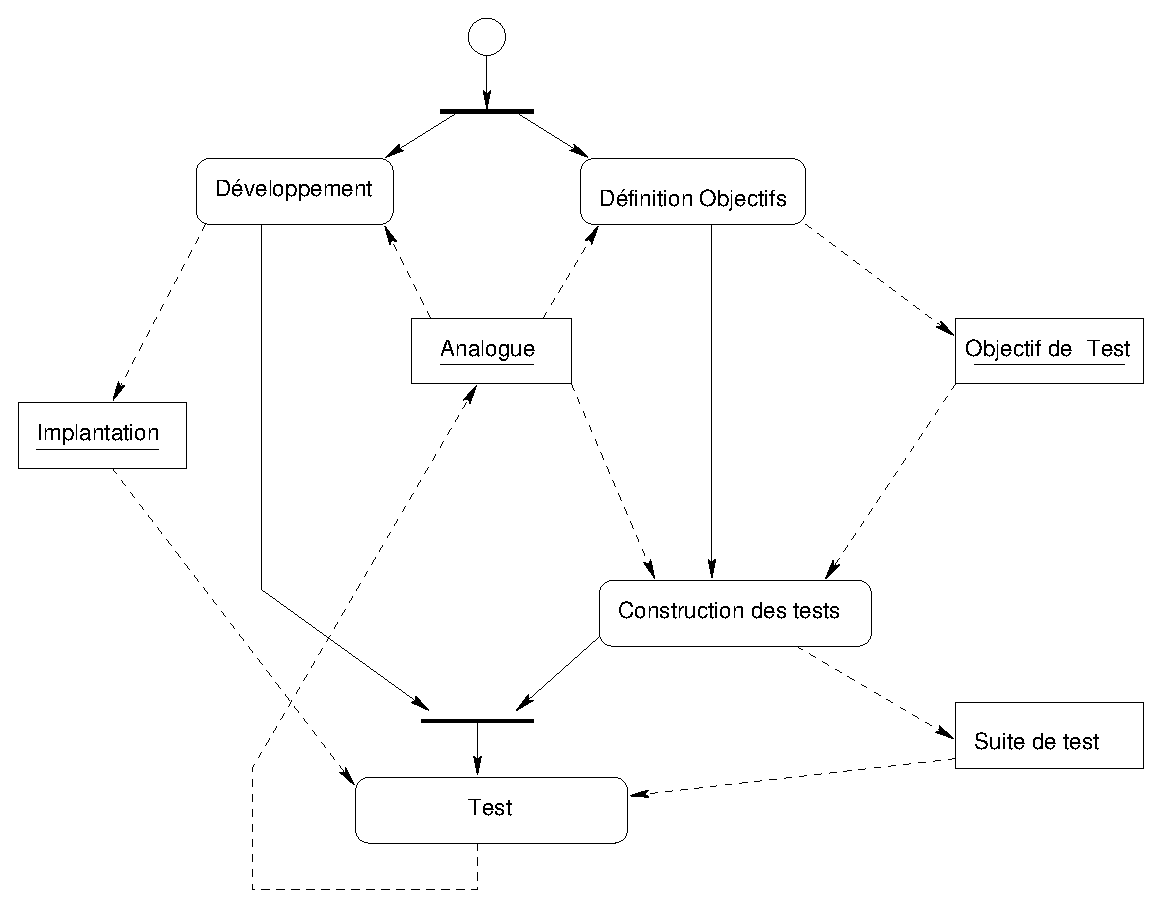
\includegraphics[width=.6\textwidth]{figures/fig-activite-test.eps}
    \caption{Activit\'e de test}
    \label{fig-activite-test}
\end{figure}

La figure \ref{fig-processtest} est une vue plus pr\'ecise de
l'activit\'e de test proprement dite, applicable \`a diff\'erents niveaux de
granularit\'e. Le processus requiert tout d'abord la validation des
tests d'int\'egration des diff\'erentes entit\'es int\'egr\'ees
dans l'\textsf{IUT}. On suppose par ailleurs que leur testabilit\'e est
contr\^ol\'ee en amont du processus. La conception des tests
d\'epend, nous l'avons vu, de l'analogue et de l'objectif fix\'e, le
premier \'etant utilis\'e par ailleurs pour construire
l'\emph{environnement de test} ou \emph{contexte de test}, c'est \`a
dire la simulation de l'ensemble des ressources dont d\'epend
l'\textsf{IUT}. Le processus d'ex\'ecution produit un verdict : si c'est un
\'echec, alors l'\textsf{IUT} contient un ou plusieurs d\'efauts qu'il est
n\'ecessaire de corriger avant de retester ; si c'est un succ\`es,
il est n\'ecessaire alors de v\'erifier que l'objectif de test est
bien atteint. Notons que dans un processus automatis\'e, les suites
de test \'etant produites  \`a partir de l'objectif de test, cette
v\'erification est imm\'ediate et toujours r\'eussie.

\begin{figure}[htbp]
    \centering
    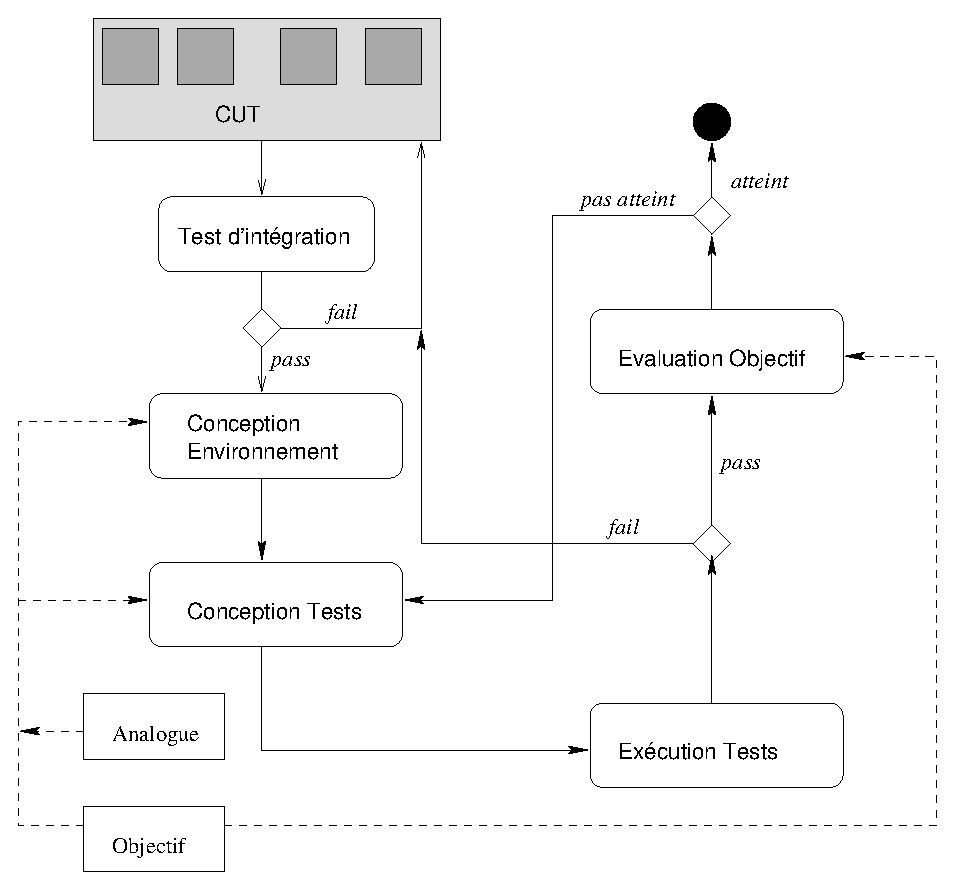
\includegraphics[width=.6\textwidth]{figures/fig-processtest.eps}
    \caption{Activit\'e de test (d\'etail)}
    \label{fig-processtest}
\end{figure}

\section{Test de conformit\'e}

Nous avons \`a la section pr\'ec\'edente fix\'e de mani\`ere
informelle la terminologie parfois confuse que l'on retrouve dans tout
ou partie des travaux sur le test. Nous avons par ailleurs identifi\'e un processus
g\'en\'eral de test unitaire prenant en compte de mani\`ere
abstraite l'ensemble des facteurs conduisant \`a la r\'ealisation
effective d'un processus de test. Il n'est clairement pas question de
passer en revue l'ensemble du domaine extr\^emement riche que
constitue le test de logiciel et nous allons donc nous attacher ici
\`a en d\'etailler la fraction qui nous int\'eresse
particuli\`erement, c'est \`a dire le test bas\'e sur des
\emph{sp\'ecifications formelles comportementales} : machines
d'\'etats finis, syst\`emes de transition, machines abstraites.

Ces travaux sont issus pour beaucoup de la probl\'ematique du test de
protocole de communication. De ce fait leur applicabilit\'e au test
de composants logiciels tels que nous les avons d\'efinis dans les
chapitres pr\'ec\'edent est presqu'imm\'ediate, les architectures de test \'etant fortement similaire. D'un point de vue
th\'eorique, ces travaux sont reli\'es d'une part au probl\`eme de
l'\'equivalence s\'emantique de processus mod\'elis\'es comme des
syst\`emes de transitions, et d'autre part \`a des recherches  sur
l'identification  de machines de 
\textsc{Moore} et plus g\'en\'eralement de transducteurs et  d'automates.

Nous effectuerons toutefois une incursion dans une autre famille de
test, le test bas\'e sur des sp\'ecifications alg\'ebriques, dans
la mesure o\`u certains travaux sur cette cat\'egorie de formalismes
ont produit des concepts pertinents pour le test de conformit\'e de
syst\`emes de transitions.

\subsection{Test alg\'ebrique}

Dans \cite{gaudel} sont  pos\'ees les bases d'une th\'eorie du
test  appliqu\'ee aux sp\'ecifications alg\'ebriques. Cette th\'eorie
est d\'evelopp\'ee dans \cite{thmarre} et par la suite reprise
notamment dans \cite{thspectest,formspectest,reqtottest,testsel,testiodata}.

On cherche ici \`a formaliser des notions
plut\^ot floues que sont la testabilit\'e, la validit\'e d'un test,
la conformit\'e, les hypoth\`eses n\'ecessaires au test. L'id\'ee
principale consiste \`a partir d'une \emph{suite de tests} exhaustive
 pour laquelle, sous une \emph{hypoth\`ese
  de testabilit\'e} de l'implantation consid\'er\'ee, on a
l'assurance que si l'implantation passe la suite de tests, elle est
conforme. Cette suite de tests \'etant g\'en\'eralement
impraticable, elle va \^etre raffin\'ee par applications successives
d'\emph{hypoth\`eses de test}, non-biais\'ees (saines) et
valides, qui permettent d'en r\'eduire la taille. Le processus s'arr\^ete lorsque l'on atteint une suite de tests
acceptable. 

Les deux types d'hypoth\`eses principales sont d\'enomm\'ees
\emph{hypoth\`ese de r\'egularit\'e} et \emph{hypoth\`ese
  d'uniformit\'e}\cite{gaudel}, elles formalisent des pratiques courantes du test
telles que le test de partitionnement, le test aux limites, la
s\'election de profondeurs de boucles ou de r\'ecursions,
... \cite{thphalippou} introduit d'autres hypoth\`eses
telles l'\emph{\'equit\'e} ou l'\emph{ind\'ependance} qui
permettent de g\'erer les probl\`emes li\'es au non-d\'eterminisme
et au parall\'elisme. 

Le couple form\'e des hypoth\`eses de test et
d'une suite de tests r\'eduite issue de l'application des
hypoth\`eses  \`a la
suite de tests exhaustive doit maintenir deux propri\'et\'es :
\begin{enumerate}
  \item il doit \^etre \emph{valide} : si l'implantation
  passe la suite de tests r\'eduite, alors elle passerait la suite de tests
  exhaustive ;
\item il doit \^etre \emph{non-biais\'e} : si
  l'implantation passe  la suite de tests exhaustive, alors elle
  passera la suite de tests r\'eduite.
\end{enumerate}
En d'autres termes, une suite de tests doit accepter toutes
les implantations  correctes et ne  pas accepter les implantations
incorrectes.

Dans \cite{formspectest}, \`a la
notion d'ensemble de test \emph{exhaustif} telle que 
d\'efinie pr\'ec\'edemment s'ajoute la notion d'ensemble complet
d\'efinie comme une suite de tests non-biais\'ee et \emph{maximale}
 : toute autre  suite de tests a un pouvoir de d\'etection plus
faible. Un point important de l'article est qu'un ensemble complet
n'est pas n\'ecessairement exhaustif et qu'il n'existe  pas
n\'ecessairement d'ensemble exhaustif pour un programme donn\'e dans
un certain cadre d'observations. Si certaines
propri\'et\'es du programme test\'e ne sont pas
observables, elles ne pourront \^etre v\'erifi\'ees par le test. Un
programme sera donc consid\'er\'e comme \emph{partiellement correct}
s'il est valide par rapport \`a une suite de tests compl\`ete.

Cette formalisation g\'en\'erale du test est reprise par ailleurs
dans la norme \textsf{IUT Z.500}\cite{itu-z500}, \og Cadre g\'en\'eral des
m\'ethodes formelles appliqu\'ees au test de conformit\'e \fg.

\subsection{Test de Machines \`a \'Etats Finis (\textsf{FSM})}

Une \emph{machine d'\'etat fini} ou \textsf{FSM} --- \emph{Finite
State Machine} --- est un n-uplet $(Q,I,O,q_0,\lambda,\delta)$
avec
\begin{itemize}
  \item $Q$ un ensemble fini d'\'etats ;
  \item $q_0 \in Q$ un \'etat initial distingu\'e ;
  \item $I$ et $O$ des alphabets finis d'\emph{entr\'ee} et de
  \emph{sortie} ;
\item $\lambda : Q\times{}I \rightarrow O^*$ la fonction partielle de sortie ;
\item $\delta : Q\times{}I \rightarrow Q$ la fonction partielle de transition.
\end{itemize}
Un \textsf{FSM} est aussi appel\'e
\emph{transducteur s\'equentiel}\cite{berstel,sakarovitch} et calcule
une  fonction rationnelle transformant un langage d'entr\'ee inclus dans $I^*$ en un 
langage de sortie inclus dans $O^*$. 

\'Etant donn\'ees une machine $A$ dont la structure est connue et
une machine $M$ dont la structure est inconnue mais dont les alphabets
sont suppos\'es identiques \`a ceux de $A$, le  \emph{test
de conformit\'e} de \textsf{FSM} consiste \`a d\'eterminer si les
deux machines calculent la m\^eme fonction en examinant les sorties
produites par $M$ pour un ensemble de mots d'entr\'ees, les
s\'equences de test.

Dans le cas g\'en\'eral o\`u $\lambda$ et $\delta$ sont des
fonctions partielles, on
distinguera\cite{sidhu-study-fsmtest} des s\'equences de test de
\emph{conformit\'e faible}, qui v\'erifient l'\'equivalence de sortie pour
les seules entr\'ees sp\'ecifi\'ees ; et des s\'equences de
test de \emph{conformit\'e forte} g\'en\'er\'ees \`a partir d'une
compl\'etion de la sp\'ecification par des transitions sans sortie
pour les lettres non sp\'ecifi\'ees dans chaque \'etat. 

Un certain nombre d'hypoth\`eses sur $M$ et de contraintes sur $A$
sont g\'en\'eralement pos\'ees pour permettre la construction
effective de s\'equences de test : minimalit\'e et/ou
d\'eterminisme de $A$, bornage du nombre d'\'etats de $M$,
correspondance des alphabets, d\'eterminisme de $M$, ...

Un tel ensemble de  \emph{s\'equences de 
v\'erification} produit un r\'esultat certain et bien \'evidemment,
hormis les cas les plus triviaux, sa construction est ardue. On
trouvera dans \cite{lee96principles} les complexit\'es de cette
construction en fonction des caract\'eristiques de $A$ : existence ou non de \emph{reset}, de \emph{s\'equences
  distinguantes}, ... Nous donnons ci-dessous quelques m\'ethodes
classiques --- ou moins classiques --- de
g\'en\'eration  de s\'equences de tests pour les \textsf{FSM}. 

Le probl\`eme de
l'\'equivalence de \textsf{FSM} remonte au moins aux travaux de Moore dans
\cite{moore-gedanken} : \'etant donn\'e une machine de Moore ---
l'implantation --- peut on \`a l'aide d'exp\'erimentations, c'est
\`a dire de s\'equences de l'alphabet d'entr\'ee, d\'eduire des
sorties produites par la machine test\'ee l'\emph{\'etat initial} de
celle-ci ? Plus g\'en\'eralement, peut-on toujours \emph{distinguer} deux machines
\`a l'aide de s\'equences de test ? La r\'eponse dans le cas
g\'en\'eral est \emph{non} : la propri\'et\'e de
distinguabilit\'e est ind\'ecidable pour une machine
arbitraire. Elle est d\'ecidable dans le cas de machines minimales de
taille born\'ee et l'on obtient m\^eme directement une borne
sup\'erieure sur la taille des suites de tests n\'ecessaires pour
distinguer deux machines donn\'ees --- \emph{ie.} une implantation inconnue
mais suppos\'ee de taille born\'ee, d\'eterministe et totalement
connexe et une sp\'ecification connue.

\subsection{S\'election des cas de test dans les \textsf{FSM} d\'eterministes}

\begin{figure}
\epsfig{width=.70\textwidth,file=figures/fig-sample-fsm.eps}
\caption{Sp\'ecification  d'un \textsf{FSM}}
\label{fig-sample-fsm}
\end{figure}

Nous pr\'esentons ici quelques m\'ethodes classiques appliqu\'ees
au test de \textsf{FSM} d\'eterministes. Cette probl\'ematique est
historiquement importante et th\'eoriquement int\'eressante, m\^eme
si en pratique son applicabilit\'e \`a la g\'en\'eration de tests
pour des probl\`emes r\'eels est faible de par la complexit\'e des
algorithmes et surtout la taille exponentielle des suites de tests
g\'en\'er\'ees. D'apr\`es \cite{lai-prototest-survey}, il semble
que seule la m\'ethode \textsf{UIO} ait \'et\'e appliqu\'ee \`a
une \'echelle industrielle dans le cadre du test de logiciels  de
t\'el\'ecommunications. 
Pour illustrer ces diff\'erentes m\'ethodes, nous utiliserons
la sp\'ecification pr\'esent\'ee dans la figure
\ref{fig-sample-fsm}, exemple tir\'e de \cite{sidhu-study-fsmtest}.

\subsubsection{Le \emph{tour de transition}}

Dans le cas d'un \textsf{FSM} fortement connexe, le tour de transition consiste
\`a construire une s\'equence de test unique par parcours de
l'ensemble des transitions du graphe du \textsf{FSM}. Cette construction peut
\^etre faite soit analytiquement par un parcours du graphe, soit par
un parcours al\'eatoire suivi d'une \'elimination des
sous-s\'equences redondantes. 

\subsubsection{La m\'ethode \textsf{W}}
\label{sec:la-methode-w}

La m\'ethode \textsf{W} a \'et\'e introduite dans \cite{chow-w-method} et
depuis abondamment reprise comme bases d'autres m\'ethodes ou
cit\'ee comme r\'ef\'erence. Le
principe de cette m\'ethode consiste \`a construire un ensemble de
s\'equences de tests, c'est \`a dire de mots appartenant \`a
l'alphabet d'entr\'ee  du \textsf{FSM} sp\'ecifi\'e, permettant de
v\'erifier pour chaque \'etat $q$, d'une part l'existence de cet
\'etat dans l'implantation sous test, d'autre part la conformit\'e
des sorties produites \`a partir de cet \'etat.

Cette m\'ethode est bas\'ee sur la construction d'un ensemble de
s\'equences \emph{caract\'eristiques} ou \emph{ensemble de distinction}, appel\'e ensemble $W$, qui
est tel que tous les \'etats du \textsf{FSM} produisent \`a partir
de $W$ un ensemble de s\'equences de sorties diff\'erent et sont
donc distinguables les uns des autres. Elle utilise aussi un ensemble
de s\'equences de \emph{couverture des transitions} du \textsf{FSM}
mod\'elis\'e, appel\'e ensemble $T$. Les deux ensembles sont
concat\'en\'es de sorte que les s\'equences d'entr\'ees
d\'efinies permettent tout d'abord d'atteindre un \'etat --- c'est
le r\^ole de $T$ --- et ensuite de v\'erifier la conformit\'e des
sorties produites dans cet \'etat --- ce que fait $W$.

La m\'ethode \textsf{W} permet aussi de v\'erifier la conformit\'e
de \textsf{FSM} dans le cas o\`u l'ensemble d'\'etats de
l'\textsf{IUT} est potentiellement plus grand que celui de la
sp\'ecification. Dans ce cas, on intercale entre les ensembles $T$ et
$W$ du \emph{bruit} sous la forme d'un ensemble des mots possibles de
taille inf\'erieure ou \'egale \`a  $m-n$, o\`u $m$ est le nombre
d'\'etats maximum estim\'e et $n$ est le nombre d'\'etat de la
sp\'ecification. 

Pour la machine pr\'esent\'ee dans la figure \ref{fig-sample-fsm},
la figure \ref{fig-seq-test-w} pr\'esente un exemple de suite de tests g\'en\'er\'ee par la m\'ethode
$W$. Notons que cet ensemble n'est pas optimis\'e : de nombreuses
s\'equences se recouvrant, il est tout \`a fait possible de
r\'eduire cette suite de tests en incluant plusieurs tests dans une
m\^eme s\'equence. 

\begin{figure}
\small 
Ensemble \textsf{W} : $\{b, aa, ba \}$.

\begin{tabular}{|ll|ll|ll|ll|}
\hline
baaabbaa & xxyxyxy &
baaabb & xxyxy &
baaabababaa & xxyxxyxyxy &
baabbba & xxyx \\
baaababaa & xxyxxyxx &
baaababbba & xxyxxyx & 
baba & xyx &
baaababaaba & xxyxxyxxyx \\
baababa & xxyxyx &
baabaaa & xxyxxy  &
baabb & xxy &
baaababab & xxyxxyxy \\
baaababa & xxyxxyx &
baaababb & xxyxxy &
baaababba & xxyxxyx &
baaababbb & xxyxxy \\
baaababaab & xxyxxyxxy &
baa & xx &
bbb &  &
baaabababa & xxyxxyxyx \\
baaababaaaa & xxyxxyxxyx &
baabba & xxyx &
baabbaa & xxyxx &
bba & x \\
baaababab & xxyxxyxy &
baabaa & xxyxx &
baaabababb & xxyxxyxyy &
bb &  \\
baabbb & xxy &
baaabababa & xxyxxyxyx &
bbba & x &
baaa & xxy \\
baaabba & xxyxyx &
baaababaaa & xxyxxyxxy &
baaabaaa & xxyxxyx &
baaabbba & xxyxyyx \\
bbaa & xx &
baaabababba & xxyxxyxyyx &
baaabab & xxyxxy &
baaabaa & xxyxxy \\
baaababbaa & xxyxxyxx &
baabab & xxyxy &
bab & xy &
baaabbb & xxyxyy \\
\hline
\end{tabular}
\caption{S\'equences de test W}
\label{fig-seq-test-w}
\end{figure}

\subsubsection{La m\'ethode \textsf{Wp}}
\label{sec:la-methode-wp}
La m\'ethode \textsf{Wp} est une am\'elioration et une g\'en\'eralisation
de la m\'ethode \textsf{W} introduite dans \cite{fujiwara-test-sel} dont
l'objectif est de r\'eduire la taille des suites de test
g\'en\'er\'ees lorsque c'est possible. 

Le principe de l'algorithme est de construire un \emph{ensemble
d'ensembles} d'identification $W=\cup_{q\in Q}W_q$, o\`u chaque $W_q$
est construit comme l'ensemble des s\'equences de $I^*$ telles que
les sorties produites \`a  partir de l'application des toutes les
s\'equences sont diff\'erentes pour tous les \'etats de $Q$. Ainsi,
au lieu de concat\'ener l'ensemble $W$ complet pour identifier chaque
\'etat apr\`es une s\'equence de tests de transitions, on peut
utiliser seulement les s\'equences d'identification propres \`a
chaque \'etat et ainsi limiter la taille des s\'equences. 

\subsubsection{La m\'ethode \textsf{UIO}}
\label{sec:la-methode-uio}

La m\'ethode \textsf{UIO} repose sur la construction, non plus de
s\'equences de distinction comme les m\'ethodes pr\'ec\'edentes,
mais sur la construction de s\'equences uniques d'entr\'ee/sortie : 
une s\'equence unique d'entr\'ee/sortie, une s\'equence \emph{UIO}
donc, pour un \'etat $q_i \in Q$ est un mot de
$(I\times{}O)^*$ tel que pour tout \'etat 
$q_j \in Q$, $UIO(q_i)\neq UIO(q_j)$. Pour tout \textsf{FSM} r\'eduit, c'est
\`a dire pour lequel aucun \'etat n'est \'equivalent pour les deux
relations $\delta$ et $\lambda$, il existe un ensemble de s\'equences
UIO.

L'utilisation des UIO \`a la place des s\'equences de distinction
permet dans la majorit\'e des cas d'obtenir des suites de tests plus
courtes, comme l'illustre la figure \ref{fig-seq-test-uio} qui
repr\'esente l'ensemble \textsf{UIO} et la suite de test
correspondante pour le \textsf{FSM}  de la figure \ref{fig-sample-fsm}.

\begin{figure}[htbp]
Ensemble \textsf{UIO} : $\{(b/1), (a/y, a/y), (b/x), (a/x), (a/y, b/x) \}$.

\begin{tabular}{|ll|}
\hline
bb &  \\
aa & xx \\
aaab & xxyx \\
aaaabbaab & xxyxyxxyx \\
aaaba & xxyxx \\
aaabaaaa & xxyxxyxy \\
aaabba & xxyxyx \\
aaab & xxyx \\
aaaabb & xxyxyx \\
aaabbb & xxyxyy \\
\hline
\end{tabular}
\caption{S\'equences de test UIO}
\label{fig-seq-test-uio}
\end{figure}

\subsection{S\'election de cas de test g\'en\'eralis\'ee}
\label{sec:selection-de-cas}
La possibilit\'e de d\'efinir des
sp\'ecifications non d\'eterministes, soit directement, soit
indirectement par une op\'eration de composition, est int\'eressante
pour les capacit\'es d'abstraction qu'elle offre. De plus, dans
le cas des \emph{machines d'\'etats finis \'etendues} ou \textsf{EFSM}\cite{bourhfir-automatic}, du fait des valeurs de
variables, ou dans celui de 
\textsf{FSM}\cite{luo-test-sel-cfsm} communiquants du fait de
l'entrelacement possible des messages, il  se pose un
probl\`eme \'evident soit d'explosion du nombre d'\'etats si l'on
cherche \`a d\'eterminiser ce type de sp\'ecification, soit
d'incapacit\'e \`a garantir un r\'esultat. 

Un certain nombre de m\'ethodes ont donc \'et\'e propos\'ees pour
s\'electionner dans ce contexte des suites de tests finies qui
permettent d'obtenir une certaine garantie quant \`a la couverture de
faute obtenue. 

\subsubsection{Approches heuristiques du test de \textsf{FSM}}
\label{sec:test-fsm-heuristic}

 \cite{lee-random-walk} pr\'esente un algorithme de
parcours al\'eatoire --- \emph{random walk} --- d'un ensemble  de \textsf{FSM}
communiquants pour couvrir les transitions de chacun des \textsf{FSM} au lieu
de couvrir l'ensemble des transitions globales. Cette approche est
\'etendue dans \cite{thzaidi} sous le nom d'algorithme
\emph{Hit-or-Jump} pour r\'esoudre le probl\`eme de l'\emph{optimum
  local}, c`est \`a dire de l'incapacit\'e d'un algorithme purement
al\'eatoire \`a trouver certaines solutions --- certains chemins ---
simples mais avec une faible probabilit\'e d'occurence qui lui
permettrait de sortir d'une boucle locale. On notera que ce
probl\`eme est bien connu dans le domaine de l'optimisation
combinatoire et qu'il a donn\'e lieu \`a un nombre de travaux de
recherche consid\'erable et notamment \`a un grand nombre
d'algorithmes heuristiques --- voir \cite{modern-heuristics} pour une
\'etude d\'etaill\'ee et r\'ecente du probl\`eme et de ses
solutions.

L'algorithme fonctionne en deux temps : une recherche locale d'une
certaine profondeur est effectu\'ee en fonction de l'\'etat courant
de mani\`ere \`a atteindre des transitions non marqu\'ees, si la
recherche est infructueuse, un saut al\'eatoire est effectu\'e  en
dehors du domaine correspondant \`a la profondeur 
choisie. Dans les deux cas, le chemin permettant d'atteindre la
transition ou l'\'etat s\'electionn\'e est construit et utilis\'e
comme cas de test.

\subsection{Test de LTS}
\label{sec:test-de-lts}

La th\'eorie du test de \textsf{LTS} --- \emph{Labelled Transition System} ou
Syt\`eme de transition \'etiquet\'e --- est introduite dans
\cite{auto-test-fm} et d\'etaill\'ee dans
\cite{thtretmans,thphalippou}. \cite{testtransbib} est 
une bibliographie comment\'ee sur le sujet. Cette th\'eorie est issue de travaux sur la s\'emantique des
alg\`ebres de processus pour lesquels on a cherch\'e \`a
caract\'eriser des relations d'\'equivalences selon un mod\`ele
id\'eal du test : \'etant donn\'e un contexte de test
d\'efinissant ce qui est observable d'un processus, deux processus
sont \'equivalents si les observations de toutes leurs ex\'ecutions
sont identiques.  \cite{sem-seq-proc} est une \'etude d\'etaill\'ee
des diff\'erentes \emph{\'equivalences observationnelles} qu'il est
possible de d\'efinir pour des LTS ne comportant pas de transition
$\tau$. Par ailleurs, la mall\'eabilit\'e du formalisme  des \textsf{LTS}
permet de d\'efinir diff\'erentes s\'emantiques d'ex\'ecution des
programmes mod\'elis\'es et donc diff\'erentes \'equivalences
possibles.


Un \textsf{LTS} $S$ est un n-uplet
$(Q,q_0,\Sigma,\rightarrow)$ avec $Q$ un ensemble d'\'etats, $q_0\in
Q$ un \emph{\'etat initial} distingu\'e, $\Sigma$ un ensemble
d'\'etiquettes de transitions ou d'\emph{actions} et $\rightarrow \subseteq Q\times{}
\Sigma\times{}Q$ une relation de transitions. \`A la diff\'erence d'un
automate, un \textsf{LTS}, dans toute sa g\'en\'eralit\'e, peut
avoir un ensemble d'\'etat infini, un alphabet infini et ne
poss\`ede pas d'\'etats terminaux. Selon certains auteurs, la notion
de processus se confond avec la notion d'\'etat : on parlera de
relations entre processus plut\^ot que de relations entre les \'etats
d'un \textsf{LTS}.  Nous utiliserons dans la section suivante la
notation $\xrightarrow[*]{\sigma}$ pour d\'esigner l'image par
la relation $\rightarrow$ et d'une s\'equence
d'\'etiquettes $\sigma$. 
On trouve aussi dans la litt\'erature la notation $q \stackrel{a}{\Rightarrow} q'$ qui
est la cl\^oture de la relation $\rightarrow$ par la transitivit\'e
des transitions \'etiquet\'ees par des actions internes, donc
inobservables. 

Nombre de relations, \`a commencer par la plus connue, la
bisimulation, sont d\'efinies  de mani\`ere \emph{coinductive}\cite{coalgebra-tutorial} comme
la plus grande relation poss\'edant certains caract\'eristiques
et contenant les \'etats initiaux.

\subsubsection{Relations d'\'equivalences dans les \textsf{LTS}}

\'Etant donn\'es deux syst\`emes $S$ et $C$ mod\'elis\'es sous la
forme des syst\`emes de transitions \'etiquet\'es
$(Q,q_0,\Sigma,\rightarrow)$  et $(P,p_0,\Lambda,\rightarrow_C)$, il
est possible de d\'efinir un grand nombre de \emph{relations
d'\'equivalence} ou de \emph{pr\'eordres} entre $S$ et $C$, ou plus
exactement entre les \'etats --- processus ---  de $S$ et de
$C$. Nous reprenons ici une fraction de la hi\'erarchie des
\'equivalences et pr\'eordres de \cite{sem-seq-proc}. Chaque
s\'emantique est d\'efinie par une \emph{relation d'\'equivalence}
not\'ee $\equiv\subseteq Q  \times{}P$, et l'on a $S\equiv C$ si et
seulement si $q_0 \equiv p_0$. 

L'\textbf{\'equivalence de traces} est la relation la plus faible de
la hi\'erarchie. Deux \'etats ou processus sont \'equivalents s'ils
peuvent produire les m\^emes s\'equences d'\'etiquettes de
transition : autrement dit, les langages clos par pr\'efixes sur les alphabets $\Sigma$ et
$\Lambda$ induits par les deux processus  sont identiques.

Si $T(q)$ d\'enote l'ensemble des traces --- clos par pr\'efixes ---
pour un \'etat $q$ quelconque, alors 
$$
C \equiv_{Tr} S \Leftrightarrow T(q_0) = T(p_0).
$$

L'\'equivalence de \textbf{traces compl\'et\'ees} est plus stricte
: elle prend en compte non seulement les --- pr\'efixes de --- traces
mais aussi les \'etats \`a partir desquelles plus aucune transition
n'est possible. Un mot $\sigma\in\Sigma^*$ est une \emph{trace compl\'et\'ee} pour un
\'etat $q$ si et seulement si $\sigma \in T(q)$ et 
$$
\forall a
\in \Sigma, \not\exists q'' \in Q,  q\xrightarrow[*]{\sigma} q'\xrightarrow{a} q''.
$$
Si $CT(q)$ d\'enote l'ensemble des traces compl\'et\'ees de $q$,
alors 
$$
C \equiv_{CT} S \Leftrightarrow CT(q_0) = CT(p_0).
$$


L'\textbf{\'equivalence de refus} est \`a
la base de la s\'emantique de \textsf{CSP}. 
Pour tout \'etat $q$, on d\'efinit l'ensemble $X(q)\subseteq \Sigma$ des \emph{refus}
de $q$ comme
$$
X(q) = \{ a\in \Sigma \mid \not\exists q'\in Q, q\xrightarrow{a}q'\},
$$
c'est \`a dire l'ensemble des actions que $q$ \emph{refuse} d'ex\'ecuter.
L'\'equivalence de refus --- appel\'ee aussi \'equivalence de
trace-refus --- entre $S$ et $C$ est d\'efinie comme :
$$
C \equiv_{Ref} S \Leftrightarrow 
\forall \sigma \in \Sigma^*,q \in Q, p\in P,\left\{
\begin{array}{lcl}
    q \equiv_{Ref} p \wedge q \xrightarrow[*]{\sigma} q' \implies p
    \xrightarrow[*]{\sigma} p' \wedge X(q') = X(p') \wedge q' \equiv_{Ref} p', \\
    q \equiv_{Ref} p \wedge p \xrightarrow[*]{\sigma} p' \implies q
    \xrightarrow[*]{\sigma} q' \wedge X(q') = X(p')\wedge q'\equiv_{Ref} p',
    \\
    q_0 \equiv_{Ref} p_0.
\end{array}\right.
$$
Les deux processus, pour \^etre \'equivalents, doivent non seulement 
pouvoir ex\'ecuter les m\^emes s\'equences d'actions, mais dans
chaque \'etat atteint, doivent refuser les m\^emes ensembles 
d'actions.  

La \textbf{bisimulation} enfin ---  ou simulation sym\'etrique ---
est l'\'equivalence la plus fine entre processus caract\'erisable
par les s\'equences de transitions et les \'etats. Cette relation a
\'et\'e d\'evelopp\'ee surtout \`a partir de \cite{milner-ccs} et
abondamment \'etudi\'ee dans le cadre du \pc, sous diverses
formes. Dans sa d\'efinition de base, elle est d\'efinie comme suit :
$$
C \sim S \Leftrightarrow 
\left\{
    \begin{array}{lcl}
        q \sim p \wedge q\xrightarrow{a} q' &\implies& \exists p', p\xrightarrow{a} p'
        \wedge q' \sim p' \\ 
        q \sim p \wedge p\xrightarrow{a} p' &\implies& \exists q', q\xrightarrow{a} q'
        \wedge q' \sim p' \\ 
        q_0 \sim p_0. &&\\
        \end{array}
\right.
$$    
Chaque couple d'\'etat de la relation doit accepter les m\^emes
actions et conduire \`a des \'etats eux-m\^emes
bisimilaires.

Il est bien s\^ur possible de d\'efinir des relations
d'\'equivalence plus fines allant jusqu'\`a l'isomorphisme des deux
syst\`emes consid\'er\'es. Signalons par ailleurs que ces
diff\'erentes \'equivalences n'ont de sens que si l'on suppose que
les processus sont non d\'eterministes, \'eventuellement
qu'ils contiennent des actions internes inobservables et que le nombre
d'\'etats est potentiellement infini. Par non
d\'eterministe, il faut entendre comme dans le cas des automates que
$\rightarrow$ est bien une relation, pas une fonction. Non
d\'eterministe peut aussi vouloir dire \emph{non d\'eterminisable} :
m\^eme si le nombre d'\'etats est fini, il est trop grand pour
esp\'erer pouvoir construire un syst\`eme d\'eterministe
\'equivalent. Dans le cas particulier des processus
d\'eterministes, on se retrouve dans la situation classique des
automates finis --- dont tous les \'etats sont terminaux --- et
toutes les \'equivalences se confondent avec l'\'equivalence de traces. 

Il est int\'eressant de souligner que les \'equivalences entre
processus sont tr\`es souvent d\'efinies comme des \emph{\'equivalences
de test}. C'est le cas dans \cite{sem-seq-proc} : les diff\'erentes
relations y sont caract\'eris\'ees par des \emph{sc\'enarios de
  test} d\'ecrivant les interactions entre un observateur et le
processus consid\'er\'e. Bien \'evidemment, plus l'observateur a de
contr\^ole sur le processus, plus il peut observer d'actions et
distinguer ses diff\'erents \'etats, plus la relation
d'\'equivalence d\'ecrite est fine. 

Comme d\'emontr\'e initialement dans \cite{obs-test-equiv}, la
puissance de l'observateur peut aussi \^etre caract\'eris\'ee par
des formules de logique modale --- logique de Hennessy-Milner --- dont
les mod\`eles sont des processus ou syst\`emes. Plus on dispose
d'op\'erateurs, plus la logique est puissante et plus les mod\`eles
deviennent pr\'ecis. 

\subsubsection{Relations de conformit\'e dans les \textsf{IOLTS}}

Le test de \textsf{LTS} s'est d\'evelopp\'e par la suite en enrichissant le
mod\`ele de base pour travailler sur des \textsf{IOLTS}, \`a partir de
l'introduction des I/O automates
\cite{intro-ioautomata,garland00using} pour d\'ecrire la
s\'emantique de processus r\'eactifs ou communiquants dans les
langages tels que LOTOS. Un \textsf{IOLTS} est simplement un
\textsf{LTS} $(Q,q_0,\Sigma,\rightarrow)$  dans lequel l'alphabet $\Sigma$
est partitionn\'e en trois : l'alphabet d'entr\'ee $\Sigma_I$,
l'alphabet de sortie $\Sigma_O$ et l'alphabet interne $\Sigma_T$ ; et pour lequel toutes les entr\'ees
sont toujours possibles. L'alphabet peut \'eventuellement
\^etre compl\'et\'e par $\delta$ exprimant le \emph{deadlock} ou la
terminaison du processus. Le test d'\textsf{IOLTS} cherche donc \`a
r\'epondre \`a la question : 
\begin{itemize}
  \item \'etant donn\'ees une sp\'ecification $S$ et une
  implantation $I$, toutes deux \'etant mod\'elis\'ees comme des
  \textsf{IOLTS}, et une relation de conformit\'e $\simeq$, est ce que
  $I\simeq S$ ?
\end{itemize}
par observation du comportement de $I$ vis \`a vis d'un testeur $T$,
lui aussi mod\'elis\'e comme un \textsf{IOLTS}. 

\paragraph{La relation \textbf{ioco}}

La \emph{relation de
  conformit\'e} utilis\'ee dans \cite{tgv} comme dans
\cite{auto-test-fm} est appel\'ee \textbf{ioco}. Soit
  $S=(Q,q_0,\Sigma,\rightarrow)$ un \textsf{(IO)LTS}, on notera ${\cal
  L}(S)$ l'ensemble des s\'equences accept\'ees par $S$ :
$$
{\cal L}(S) = \{\sigma \in \Sigma^*, \exists q \in Q,
q_0\stackrel{\sigma}{\Rightarrow} q\}.
$$
Cette relation est d\'efinie comme :
$$
I \ioco S \iff \forall u\in {\cal L}(S), \{a \in \Sigma_O \mid u.a \in
  {\cal L}(I)\} \subseteq \{a \in \Sigma_O | u.a \in
  {\cal L}(S)\}.
$$
Autrement dit, l'implantation ne peut produire plus de sorties que
pr\'evues par la sp\'ecification. On notera que dans \cite{tgv}, les entr\'ees et
sorties sont vues du point de vue de l'\emph{environnement} de l'\textsf{IUT} et
donc invers\'ees par rapport \`a cette d\'efinition.
\cite{thphalippou} d\'efinit un certain nombre d'autres
relations de conformit\'e possibles, nomm\'ees $R_1$ \`a
$R_5$ mais qui peuvent s'exprimer dans le m\^eme cadre. 

De m\^eme que l'on \'etablit une hi\'erarchie de relations de
d'\'equivalence observationnelle entre processus mod\'elis\'es par
des \textsf{LTS}, on peut \'etablir une hi\'erarchie entre processus
mod\'elis\'es par des \textsf{IOLTS}. Cette hi\'erarchie est
d\'evelopp\'ee dans  \cite{tgenioq} o\`u plusieurs relations
d'implantation sur des \textsf{IOLTS} sont \'etudi\'ees :  les relations de \emph{test
  d'entr\'ee-sortie}  $\leq_{iot}$, de test d'entr\'ee-sortie
conforme $\mathbf{ioconf}$, de refus d'entr\'ee-sortie $\leq_{ior}$
et de refus d'entr\'ee-sortie conforme $\mathbf{ioco}$. 

Ces relations
sont toutes caract\'eris\'ees par l'inclusion des \emph{sorties}
possibles apr\`es une trace mais se distinguent par l'ensemble de
traces sur lequel la relation d'inclusion doit \^etre
v\'erifi\'ee. La notion de \emph{quiescence} est ici essentielle :
un \'etat est quiescent si aucune \emph{sortie} n'est possible dans
cet \'etat. Pour faciliter la construction des relations de
conformit\'e, on va donc mod\'eliser la quiescence par une
transition sp\'eciale \'etiquet\'ee $\delta$. Cette transition peut
correspondre soit \`a un refus de l'ensemble des sorties possible,
soit comme une lettre terminale et peut-\^etre pr\'evue ou non dans
la sp\'ecification.  La distinction
entre $\leq_{iot}$ et $\mathbf{ioconf}$ permet d'\'eviter la
mod\'elisation explicite de toutes les entr\'ees dans la
sp\'ecification. Celle-ci est alors un simple \textsf{LTS} \'etiquet\'e
par les lettres d'entr\'ees et de sorties et non pas un \textsf{IOLTS} pour
lequel \emph{toutes} les entr\'ees sont toujours possibles. C'est
l'approche la plus courante. 

\paragraph{Autres relations}

Dans \cite{petrenko-testlts-io}, les auteurs introduisent
la notion d'\'equivalence de traces avec quiescence et file ---
\emph{queued-quiescent trace equivalence}. Le testeur est ici divis\'e en deux parties, un \emph{testeur
des entr\'ees} qui va fournir une s\'equence d'entr\'ees \`a l'\textsf{IUT} et
un testeur des sorties qui va valider les sorties produites par
l'\textsf{IUT} en fonction de celles attendues dans la
sp\'ecification, 
produisant un verdict \texttt{pass} ou \texttt{fail}. Le principe 
consiste \`a d\'efinir pour une s\'equence de test $\alpha$ donn\'ee, les
sorties possibles en fonction de l'atteinte d'\'etats quiescents,
c'est \`a dire d'\'etats dans lesquels seules des entr\'ees sont
possibles.

Sous r\'eserve que la sp\'ecification ne poss\`ede pas de cycle de
sorties, on peut construire  un ensemble de cas de test fini par
\'enum\'eration des s\'equences quiescentes-enfil\'ees de taille
inf\'erieure \`a $k$ o\`u $k$ est la taille de la plus longue
s\'equence de sortie dans l'ensembles des traces quiescentes de
l'\'etat initial. La relation
d'\'equivalence de traces quiescentes-enfil\'ees est moins fine que
la relation $\ioco$ d\'efinie dans \cite{auto-test-fm}.

Cette id\'ee est \'etendue pour permettre de distinguer les cas
o\`u des \'etats quiescents interm\'ediaires peuvent appara\^{\i}tre
pour une s\'equence $\alpha$ en introduisant des couples testeurs
d'entr\'ees-testeurs de sortie pour chaque sous-s\'equence de
$\alpha$ menant \`a un \'etat quiescent. On peut remarquer que cette
construction revient \`a travailler sur une sp\'ecification qui est
la cl\^oture par une relation d'ind\'ependance entre les entr\'ees
et les sorties situ\'ees entre deux \'etats quiescents. 
D'autres relations sont d\'efinies dans le cadre du test r\'eparti :
elles sont d\'ecrites \`a la section \ref{sec:le-test-reparti}. 

\subsection{Algorithmes de tests dans les \textsf{IOLTS} }

Si les \textsf{IOLTS} fournissent une th\'eorie compacte et globale du test,
il n'en reste pas moins vrai que l'application de cette th\'eorie de
la conformit\'e suppose de r\'ealiser une s\'election de tests
comme pour les autres formalismes et mod\`eles pr\'esent\'es pr\'ec\'edemment.

\subsubsection{TGV}
\label{sec:tgv}
Le principe de construction des cas de test dans TGV\cite{tgv} est de
r\'ealiser un produit de synchronisation \`a la vol\'ee entre la
sp\'ecification $S$ et l'\emph{objectif de test} $TP$. Ce dernier est un \textsf{LTS}
acyclique complet sur l'alphabet de la sp\'ecification dont les \'etats sont
marqu\'es $\mathtt{Accept}$ ou $\mathtt{Reject}$.  Un
objectif  de test $TP$ doit de plus poss\'eder la propri\'et\'e d'\^etre
contr\^olable : si un \'etat autorise un \'ev\'enement de sortie,
alors aucun autre \'ev\'enement n'est permis. En d'autres termes,
l'objectif de test $TP$ doit \^etre \emph{d\'eterministe au sens du
  test}. L'objectif de test repr\'esente une partie du comportement
sp\'ecifi\'e de l'IUT que l'on souhaite express\'ement
v\'erifier. Les objectifs de test sont d\'etermin\'es par le
testeur en fonction de la strat\'egie globale de v\'erification du projet.

Les diff\'erentes \'etapes de l'algorithme de construction
pr\'esent\'e dans \cite{tgv} sont les suivantes :
\begin{enumerate}
  \item construction du produit de mixage $TP\times{}S$. Ce produit
    synchrone est r\'ealis\'e en construisant un \emph{automate de
    suspension} : les diff\'erentes formes  de quiescence que sont le
    blocage et  l'attente d'une entr\'ee sont transform\'ees en boucles
    \'etiquet\'ees par la lettre $\delta$ ;
  \item construction d'un graphe dirig\'e acyclique repr\'esentant le cas de test avec un
    \emph{pr\'eambule}, un \emph{corps} et un \emph{postambule}. Le
    pr\'eambule initialise le cas de test pour atteindre un \'etat
    contenant des transitions de $TP$. Le postambule est  un chemin
    de \emph{reset}, permettant de revenir \`a l'\'etat initial de $S$
    apr\`es avoir atteint l'\'etat $\mathtt{Accept}$ dans $TP$. Au
    cours de cette \'etape, les conflits de contr\^olabilit\'e sont
    supprim\'es en \'elaguant les branches n\'ecessaires ;
  \item d\'efinition des verdicts associ\'es \`a chaque transition :
    \begin{itemize}
      \item \texttt{Pass} pour une transition vers un \'etat du postambule
        tel que $S$ est dans son \'etat initial,
      \item \texttt{(Pass)} pour une transition menant vers le
        postambule,
      \item \texttt{Inconclusif} pour une sortie autoris\'ee par la
        sp\'ecification mais non pr\'esent dans $TP$,
      \item \texttt{Fail} pour toute transition de sortie non pr\'evue par
        la sp\'ecification ;
    \end{itemize}
  \item d\'ecoration des \'etats par des timers et des transitions
    $\delta$ pour les boucles de transitions internes. Un \emph{timer} est associ\'e \`a
    chaque sortie possible dans un \'etat et annul\'e quand la sortie
    n'est plus possible, soit parce qu'elle a eu lieu, soit parce
    qu'elle n'est plus autoris\'ee  par la sp\'ecification. Ces timers
    permettent de g\'erer les cas  d'entrelacement des sorties.
\end{enumerate}
La particularit\'e de \textsf{TGV} est d'effectuer ces
diff\'erentes \'etapes \`a la vol\'ee et donc de ne pas avoir
\`a d\'eplier l'ensemble du graphe de la sp\'ecification  pour
construire l'ensemble de test. 

\'Etant donn\'e la sp\'ecification pr\'esent\'ee en partie gauche
de la figure \ref{fig-sample-iolts} et l'objectif de test en partie
droite de la m\^eme figure, implicitement compl\'et\'e par
l'alphabet de ${\cal S}$, le produit de
synchronisation entre les deux donne la figure
\ref{fig-sample-iolts-synch}. Ce produit de synchronisation est
l\'eg\`erement diff\'erent de celui r\'ealis\'e par \textsf{TGV} car il
contient encore des transitions internes marqu\'ees \verb|^t|.
Les \'etats terminaux marqu\'es d'un cercle blanc repr\'esentent
les tests \emph{r\'eussis}, les \'etats non coaccessibles --- par
exemple l'\'etat 28 --- 
repr\'esentent des tests \emph{\'echou\'es} et les \'etats
interm\'ediaires des test \emph{non-concluants}.
L'exemple pr\'esent\'e sur ces diff\'erents sch\'emas est tir\'e
de \cite{tgv}. 

\begin{figure}[htbp]
    \centering
    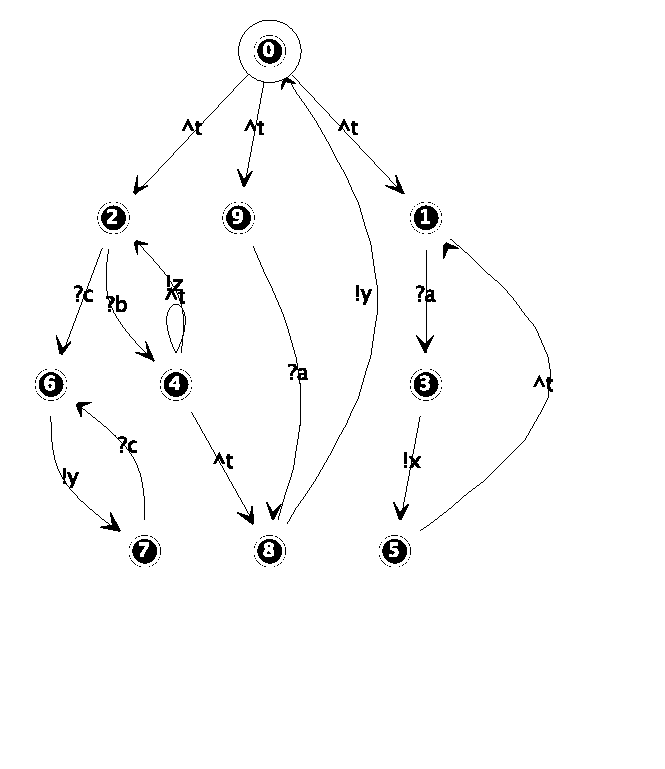
\includegraphics[width=.45\textwidth]{figures/fig-sample-iolts.eps}
    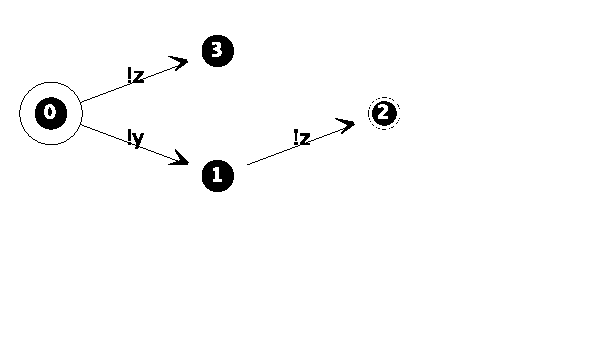
\includegraphics[width=.45\textwidth]{figures/fig-sample-iolts-tp.eps}
    \caption{Sp\'ecification ${\cal S}$ \& Objectif de test ${\cal O }$}
    \label{fig-sample-iolts}
\end{figure}

\begin{figure}[htbp]
    \centering
    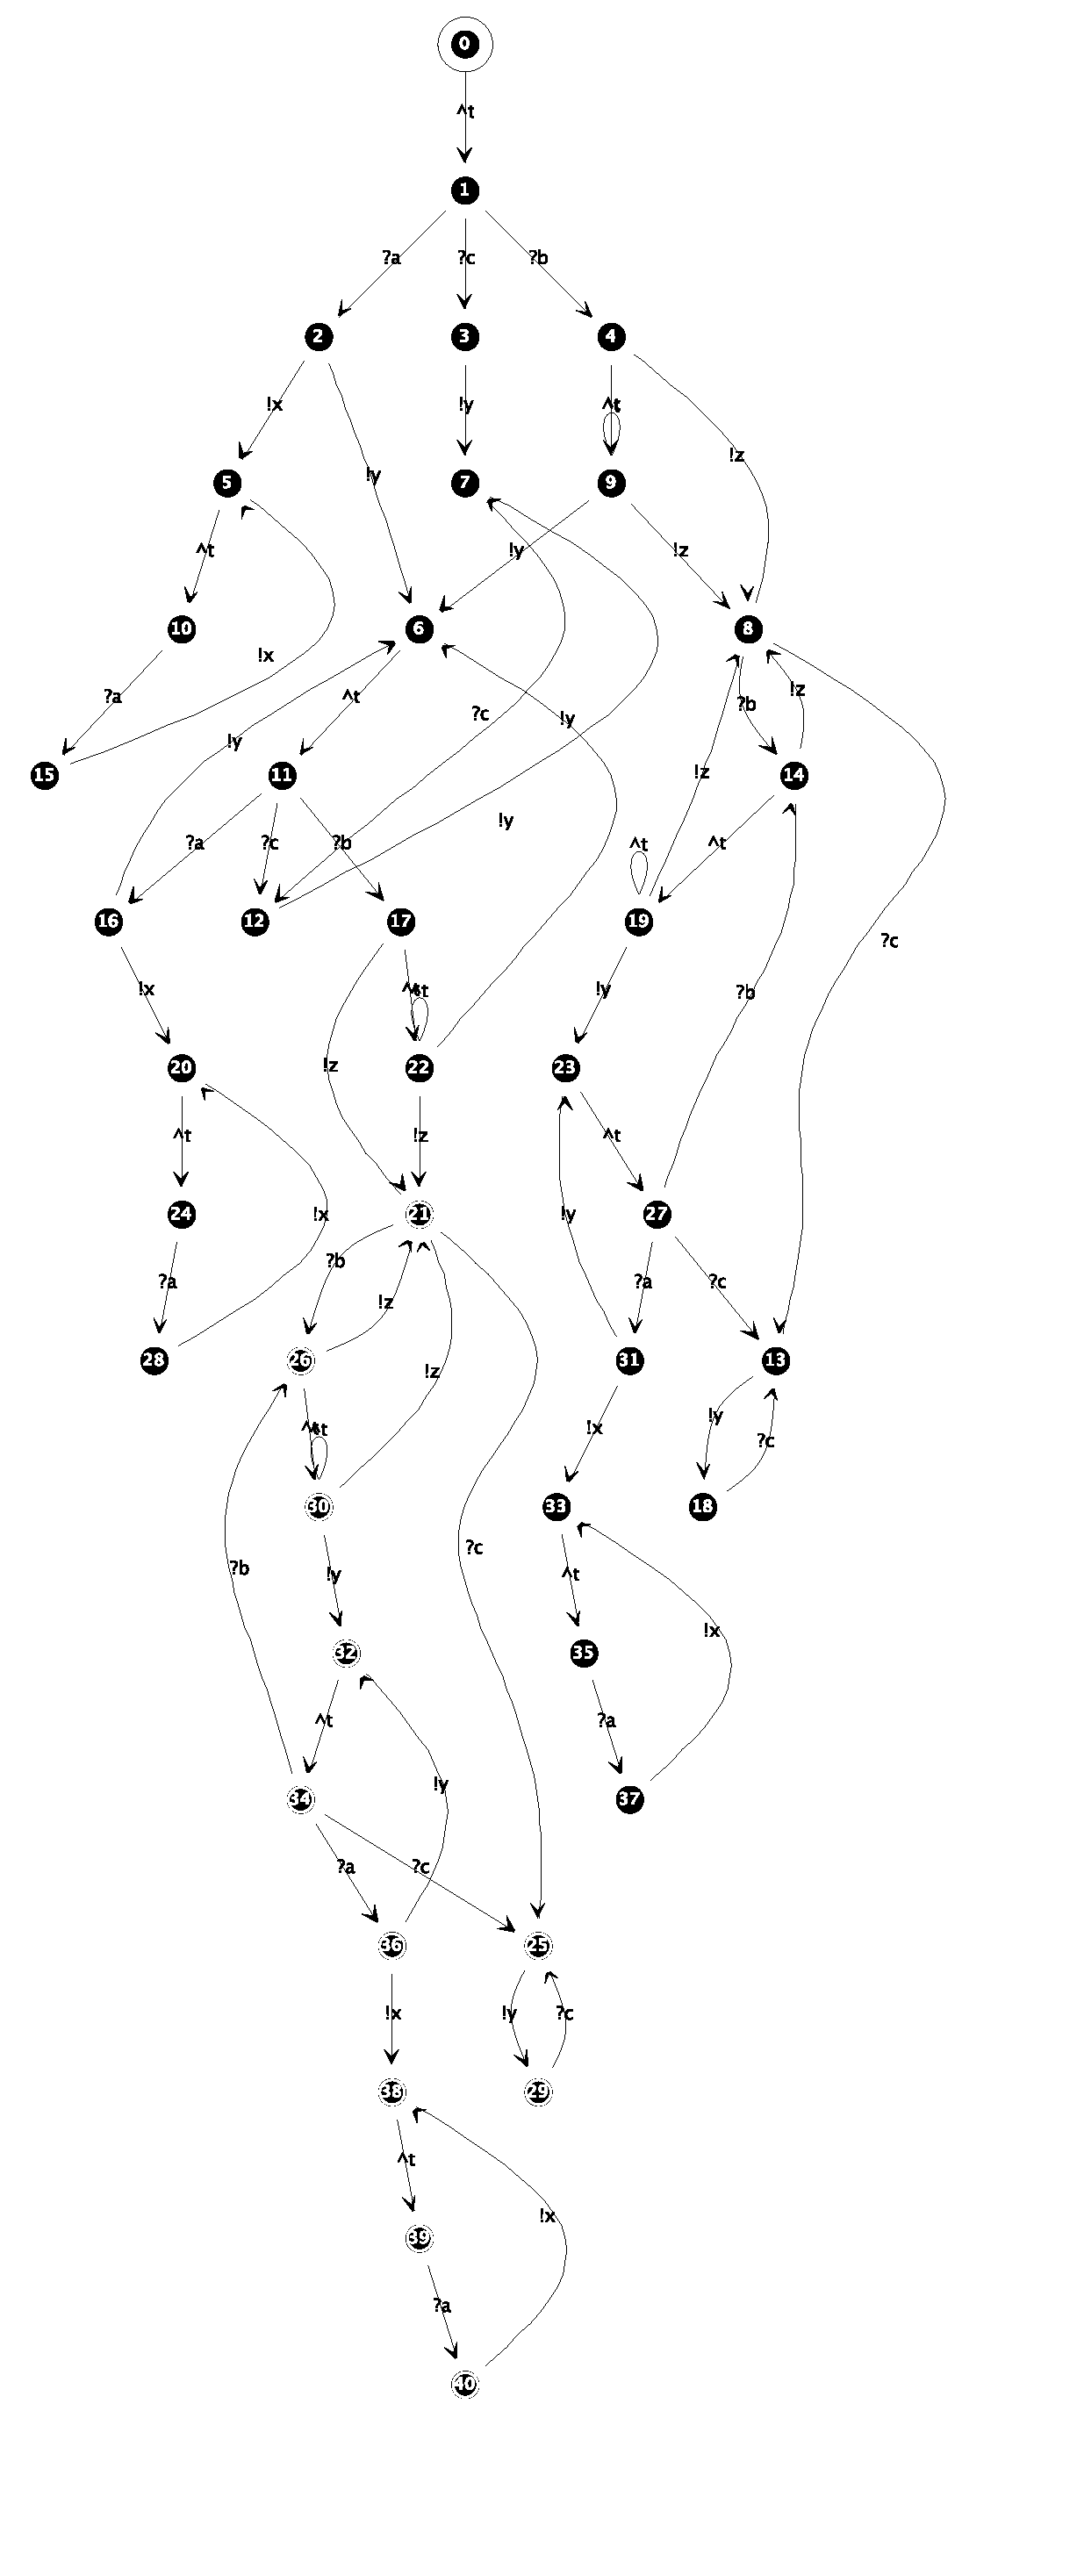
\includegraphics[height=.9\textheight]{figures/fig-sample-iolts-synch.eps}
    \caption{Synchronization ${\cal TP}\|{\cal S}$}
    \label{fig-sample-iolts-synch}
\end{figure}

Sous r\'eserve d'une hypoth\`ese d'\emph{\'equit\'e} --- born\'ee
-- de l'implantation, cette construction permet de s'assurer de la
validit\'e d'une implantation m\^eme dans  les cas de
non-d\'eterminisme de cette derni\`ere. 
La s\'election repose donc sur le choix d'un objectif de
test, solution que l'on retrouve par ailleurs dans d'autres approches
bas\'ees sur ce m\^eme outil\cite{test-pf,stg}.

\subsubsection{\textsc{TorX}}

La g\'en\'eration des cas de tests dans l'outil \textsc{TorX} est
bas\'ee sur les travaux th\'eoriques de
\cite{thtretmans}. Contrairement \`a \textsf{TGV}, la g\'en\'eration et
l'ex\'ecution des cas de test sont effectu\'es concurremment selon
un processus non-d\'eterministe\cite{tgenioq} dit aussi test \emph{online}. La notion d'objectif de test est
absente mais le processus peut \^etre guid\'e par le testeur. 

Le cas de test est un arbre \'etiquet\'e par l'alphabet de la
sp\'ecification auquel on ajoute une transition de \emph{quiescence}
pour g\'erer les comportements de blocage. Il est construit
r\'ecursivement par application non-d\'eterministe des trois
r\`egles suivantes \`a partir d'un \'etat initial $q_0$ :
\begin{enumerate}
  \item l'\'etat courant est un \'etat terminal \texttt{pass} ;
  \item \textbf{une} transition d'entr\'ee \emph{valide} est ajout\'ee \`a
  l'\'etat courant, l'\'etat atteint devient le nouvel \'etat
  courant ;
\item \textbf{toutes} les transitions de sortie possibles plus une transition
  $\delta$ sont ajout\'ees \`a l'\'etat courant, les \'etats
  atteints $q_i$ sont ensuite trait\'es successivement en fonction de
  l'ensemble des transitions \'etiquet\'ees des lettres de sorties
  $o_i\in \Sigma_O$ ou une \'etiquette de quiescence $\delta$ :
  \begin{itemize}
    \item si $o_i\not\in \mathrm{Out}(q)$, l'\'etat est marqu\'e
      \texttt{fail},
    \item si $\delta\not\in \mathrm{Out}(q)$, l'\'etat est marqu\'e
      \texttt{fail},
    \item sinon, l'\'etat atteint devient le nouvel \'etat courant.
  \end{itemize}
\end{enumerate}

\subsection{S\'election de cas de tests pour les \textsf{IOLTS}}
\label{sec:selection-iolts}

Une premi\`ere approche est esquiss\'ee dans \cite{thtretmans},
chapitre 6, o\`u l'auteur propose un cadre th\'eorique au probl\`eme
de la s\'election : une \emph{fonction de valuation} permet d'attribuer \`a
chaque suite de tests $K$ une valeur d\'ependant de son pouvoir de
d\'etection de d\'efauts. Cette fonction est pond\'er\'ee par une partition
de l'espace des \'etats et des erreurs induite par les diff\'erentes
suites de test. Une \emph{fonction de co\^ut} est aussi calcul\'ee
en raison de la taille des suites de tests g\'en\'er\'ees, un
arbitrage \'etant ensuite effectu\'e par le testeur entre ces deux
valeurs. Toutefois, aucune solution concr\`ete n'est propos\'ee pour
le calcul, essentiel, de la fonction de valuation, sauf dans le cas
d'une s\'election bas\'ee sur un objectif de test.

Dans \cite{curgus-analytic-test}, une m\'ethode de s\'election de
cas de tests bas\'ee  sur la d\'efinition d'une \emph{m\'etrique}  de l'espace des
s\'equences de test est propos\'ee. Il est alors possible de
s\'electionner des cas de tests parmi un ensemble donn\'e assurant
une certaine couverture, c'est \`a dire une distance maximale entre
les s\'equences s\'electionn\'ees et l'ensemble des s\'equences
possibles. Le principal inconv\'enient de l'algorithme propos\'e est
qu'il n\'ecessite de partir d'une suite de test, par exemple un
objectif de test. 

Dans \cite{spec-coverage-select,pyhala-test-selection}, la s\'election des cas de test se
fait en utilisant un crit\`ere de couverture de la sp\'ecification,
par exemple la couverture de transitions.  L'algorithme pr\'esent\'e
est similaire \`a l'heuristique de recherche locale pr\'esent\'ee
ci-dessus pour les \textsf{FSM} : l'algorithme cherche \`a maximiser les
transitions couvertes par une recherche des transitions ex\'ecutables
dans son voisinage et effectue un choix al\'eatoire
dans le cas contraire. \cite{kervinen-heuristic} est un raffinement de ces principes :
une fonction d'\'evaluation est associ\'ee \`a chaque transition
courante et \`a chaque \'etat en fonction d'un objectif de
couverture, la valeur d'un \'etat prenant par ailleurs en compte la
valeur des \'etats accessibles \`a partir de
celui-ci jusqu'\`a une certaine profondeur. Diff\'erentes strat\'egies de s\'election sont ensuite
possibles, une strat\'egie dite pessimiste qui consid\`ere que l'\textsf{IUT}
s\'electionne en priorit\'e les transitions avec la plus faible
valuation, une strat\'egie adaptative qui modifie la valeur des
transitions en fonction des transitions d\'ej\`a parcourues.

 \cite{yannakakis-test-opt-games} est une synth\`ese
r\'ecente des approches heuristiques \og modernes\fg pour la
s\'election des cas de test dans les \textsf{IOLTS} : il examine
successivement la mod\'elisation du probl\`eme comme un jeu \`a
deux joueurs, comme un probl\`eme d'optimisation combinatoire et
comme un probl\`eme d'apprentissage supervis\'e. L'auteur rappele un
certain nombre de r\'esultats de d\'ecidabilit\'e et de
complexit\'e sur ces diff\'erentes mod\'elisations. La
mod\'elisation du probl\`eme du test comme un jeu est aussi \`a la
base du test d'\emph{Abstract State Machines} pr\'esent\'e dans
\cite{blass-test-game}. 

Ces diff\'erents travaux s'inspirent de crit\`eres de couverture
utilis\'es dans le test structurel (voir section
\ref{sec:test-structurel})  pour s\'electionner  de mani\`ere
objective et contr\^ol\'ee des suites de tests. Nous pensons que
cette approche est, d'un point de vue pratique, tr\`es
int\'eressante, surtout lorsqu'on cherche \`a int\'egrer dans le
processus de s\'election de cas de tests les donn\'ees. Le chapitre
\ref{cha:test} consacr\'e au test d\'efinira une proc\'edure de s\'election pour les
automates \textsf{FIDL} qui est clairement inspir\'ee  de ces
approches.

\cite{testiodata,gaudel-unitheory} unifient deux formalismes, les \textsf{IOLTS}
et les sp\'ecifications alg\'ebriques dans une m\^eme
d\'emarche. Les sp\'ecifications sont ici des \textsf{IOLTS} 
dont les messages comportent des donn\'ees vues comme des types
alg\'ebriques abstraits. L'ensemble de test exhaustif est construit
\`a partir d'un certain nombre d'hypoth\`eses de testabilit\'e de
l'implantation :
\begin{itemize}
  \item l'implantation est un \textsf{IOLTS} acceptant toujours toutes les
  entr\'ees ;
\item le non-d\'eterminisme est limit\'e par une hypoth\`ese
  d'\'equit\'e born\'ee, c'est \`a dire qu'il existe un entier $n$ tel
  que $n$ ex\'ecutions d'un test assure que tous les choix
  non-d\'eterministes auront \'et\'e faits ;
\item toutes les actions parall\`eles sont ind\'ependantes ;
\item l'implantation dispose d'un \emph{reset} correctement
  implant\'e ;
\item l'\textsf{IOLTS} repr\'esentant l'implantation est fortement convergent :
  il n'existe pas de chemin infini de transitions \'etiquet\'ees par
  un \'ev\'enement interne.
\end{itemize}
L'ensemble de test exhaustif est alors d\'efini comme  l'ensemble des
s\'equences de message de  la sp\'ecification compl\'et\'ees par
 les sorties non autoris\'ees
--- compte tenu de l'\'ev\'enement particulier $\delta$ d\'enotant
l'absence de sorties.  \`A partir de cette d\'efinition, on utilise une
variante de l'algorithme non-d\'eterministe pr\'esent\'e ci-dessus dans la section
consacr\'ee \`a \textsc{ToRX} pour construire des cas de tests
appartenant \`a cet ensemble. 

La construction de la suite concr\`ete de tests d\'epend en fait
d'hypoth\`eses faites sur les param\`etres des messages. \`A partir
d'une description symbolique, on va tout
d'abord d\'efinir une longueur maximale de test (hypoth\`ese de
r\'egularit\'e) permettant de couvrir l'ensemble des \emph{op\'erations}
possibles sur le type des param\`etres, c'est \`a dire tous les
constructeurs du type de donn\'ees en question. Pour am\'eliorer la
couverture des diff\'erents cas, on va d\'eplier les op\'erations
selon les diff\'erentes r\`egles disponibles. Enfin, les valeurs
sont instanci\'ees par r\'esolution des contraintes r\'esultant des
pr\'edicats de gardes pour les diff\'erentes transitions
non-autoris\'ees, c'est \`a dire g\'en\'eralement par
r\'esolution d'une conjonction des n\'egations des diff\'erentes
conditions d'activation de transitions de sorties. 

\subsection{Le test r\'eparti}
\label{sec:le-test-reparti}

\begin{floatingfigure}{.45\textwidth}
    \epsfig{width=.4\textwidth,file=figures/fig-archi-dist-test.eps}
    \caption{Architecture de test r\'eparti}
    \label{fig-archi-dist-test}
\end{floatingfigure}

S'il n'existe pas \`a notre connaissance de \emph{th\'eorie} du test de
composants ou d'architectures logiciels, au sens o\`u nous l'entendons
dans cette th\`ese, il existe par contre de nombreux travaux sur le
probl\`eme du \emph{test r\'eparti}. Dans le test r\'eparti,  le testeur n'est plus  monolithique
mais peut interagir avec le programme test\'e au travers de plusieurs
\emph{points de contr\^ole et d'observation} ou  \textsf{PCO}
\'eventuellement r\'epartis sur un r\'eseau. On remarque que cette 
situation  correspond au probl\`eme du test d'un composant
pouvant offrir et requ\'erir plusieurs interfaces et poss\'eder
plusieurs fl\^ots de contr\^ole  plus ou moins ind\'ependants.

On distinguera le \emph{test r\'eparti coordonn\'e}, dans lequel les
testeurs  ont la possibilit\'e de se synchroniser entre eux du \emph{test r\'eparti pur}
dans lequel les testeurs ne disposent pas de cette facilit\'e. La
figure \ref{fig-archi-dist-test} repr\'esente sch\'ematiquement ces
architectures de test : le trait pointill\'e entre les testeurs
n'existe pas dans une architecture de test r\'eparti pur.

\subsubsection{Test r\'eparti pur}

Le test r\'eparti pur a \'et\'e \'etudi\'e en particulier dans
\cite{luo-tgen-dist,sarikaya-proto-test,hierons-check-synch} pour ce
qui concerne le mod\`ele des (E)\textsf{FSM}. Nous ne connaissons pas
d'\'etude concernant ce probl\`eme appliqu\'e au test d'\textsf{IOLTS}.
Dans cette configuration, des d\'efauts peuvent appara\^{\i}tre de par
la nature partielle des observations et du contr\^ole que chaque
testeur a de l'implantation sous test : il peut ne pas y avoir de lien
direct entre une entr\'ee sur un \textsf{PCO} donn\'ee et les sorties sur ce
PCO, ce qui revient \`a dire qu'on ne peut pas toujours conna\^{\i}tre
l'\'etat global du syst\`eme test\'e \`a partir de ses \'etats
locaux, un probl\`eme classique de l'algorithmique distribu\'ee. 

Dans tous le cas, le syst\`eme est repr\'esent\'e par un \textsf{FSM} dont
l'alphabet d'entr\'ee et de sortie est partitionn\'e entre les
diff\'erents \textsf{PCO} du syst\`eme, les transitions peuvent donc mettre
en \oe uvre des ports diff\'erents pour l'entr\'ee et la sortie. 

\cite{luo-tgen-dist,sarikaya-proto-test} cherchent \`a construire une
s\'equence de test de type \emph{tour de transition} qui sera dite
\emph{synchronisable} : une s\'equence est synchronisable si toutes
les paires de transitions  de la
s\'equence sont synchronisables c'est \`a dire si l'on peut toujours
les ordonner localement sur un ou plusieurs ports. Il existe bien s\^ur des cas o\`u une telle s\'equence
n'existe pas, ce qui signifie que l'on ne peut pas toujours
v\'erifier la conformit\'e d'une \textsf{IUT} dans une architecture
distribu\'ee pure. 

Sur le m\^eme mod\`ele,
\cite{hierons-check-synch} cherche \`a construire une s\'equence de
v\'erification selon l'algorithme \textsf{UIO}. Un probl\`eme connexe \`a la
synchronisation est celui des d\'ecalages de sortie, dans le cas
o\`u une sortie correcte observable sur un port peut appara\^{\i}tre
sur deux transitions cons\'ecutives dont l'une n'est pas d\'ependante
d'une entr\'ee sur le m\^eme port. La m\'ethode pr\'esent\'ee
est de construire des s\'equences d'UIO synchronisables pour chacun
des ports et chacun des \'etats du syst\`eme en transformant le
graphe de la sp\'ecification initiale de mani\`ere \`a identifier
les probl\`emes de synchronisation.  Comme pr\'ec\'edemment, la
possibilit\'e de construire un ensemble de test d\'epend fortement
de la structure initiale de la sp\'ecification.

\subsubsection{Test r\'eparti synchronis\'e}

Le cas du test r\'eparti synchronis\'e a \'et\'e comparativement
plus \'etudi\'e car il correspond \`a une situation plus favorable
pour le testeur et  r\'ealiste dans un contexte de test en cours
de d\'eveloppement. Cette architecture est similaire au test
centralis\'e puisque les testeurs  
ont toute latitude pour reconstruire en communiquant un \'etat global
\`a partir de leurs \'etats locaux.

Dans \cite{cacciari-dist-test}, ce probl\`eme est \'etudi\'e dans
l'univers des \textsf{FSM} et le principal r\'esultat est un algorithme
permettant de synchroniser des testeurs locaux avec un nombre garanti
minimal de messages \'echang\'es.

Dans le monde des \textsf{IOLTS},
\cite{ulrich-concur-testing} introduit une
s\'emantique concurrente non-entrelac\'ee pour l'ordonnancement
des messages entre les diff\'erents testeurs. La construction de
s\'equences de test est
bas\'ee sur la construction de r\'eseaux de Petri \`a partir de
sp\'ecifications \textsf{IOLTS} puis sur le \emph{d\'epliage} du r\'eseau global
obtenu \`a partir des sp\'ecifications locales de mani\`ere \`a
obtenir un graphe dirig\'e acyclique des pr\'efixes
d'\'ev\'enements d\'ependants les uns des autres. Le d\'epliage
s'arr\^ete lorsque des configurations d'\'ev\'enements d\'ej\`a
atteintes sont rencontr\'ees, les \'ev\'enements concurrents
introduisant des points de branchement dans le d\'epliage. Cette
construction est applicable uniquement en l'absence d'interblocage
 dans la sp\'ecification, une propri\'et\'e qui peut
\'eventuellement \^etre v\'erifi\'ee par
\emph{model-checking}. Le graphe de d\'ependance d\'epli\'e peut
ensuite \^etre utilis\'e pour g\'en\'erer des s\'equences de
test de conformit\'e qui sont ensuites projet\'ees sur les testeurs
locaux pour ex\'ecution. 

Ce m\^eme principe est appliqu\'e dans \cite{jard-synth-dist-test}
pour \'etendre les principes de la g\'en\'eration de cas de tests
de \textsf{TGV} au cas des testeurs r\'epartis. Le formalisme utilis\'e est
l\'eg\`erement diff\'erent et plus complexe que dans \cite{ulrich-concur-testing} mais
surtout le principe du d\'epliage des \'ev\'enements concurrents
est dirig\'e par l'\emph{objectif de test}. De plus, les
d\'ependances entre \'ev\'enements sur des testeurs diff\'erents
sont contr\^ol\'ees par l'insertion de messages de synchronisation
entre testeurs comme dans \cite{cacciari-dist-test}. Notons que dans
tous les cas cit\'es, il est n\'ecessaire de construire la
sp\'ecification globale de l'IUT.

La formalisation de la notion de testeur r\'eparti et des relations
d'implantation correspondantes est d\'etaill\'ee dans
\cite{heerink-miots-test,heerink-factor-miots}. L'auteur d\'efinit un
\emph{MIOTS}, c'est \`a dire un \textsf{IOLTS} dont les alphabets d'entr\'ee
et de sortie sont partitionn\'es sur un ensemble de canaux --- les
PCO ---, et une relation d'implantation \textbf{mioco} similaire \`a
\textbf{ioco} --- un pr\'eordre sur les ensembles de traces-refus
---- mais param\'etr\'ee par la partition des alphabets. 

Bien que nous ayons remarqu\'e l'absence d'outils th\'eoriques
propres au test de composants architecturaux,
\cite{composition-testing-ioco} s'est int\'eress\'e au probl\`eme
du test de \emph{composants} en g\'en\'eral dans le cadre de la
relation \textbf{ioco} et des \textsf{IOLTS}. Il montre que sous l'hypoth\`ese
de certaines restrictions, il n'est pas n\'ecessaire de retester
le r\'esultat de la composition de deux composants qui sont
\textbf{ioco} conformes \`a leur sp\'ecification respectives. La
composition est ici entendu au sens d'un produit de synchronisation
des alphabets internes aux deux composants suivi d'une projection.

\section{Test structurel \& Crit\`eres de couverture}
\label{sec:test-structurel}

Bien qu'il ne constitue pas l'objet principal de notre \'etude, cette
section pr\'esente une synth\`ese des techniques de test dit
structurel. Premi\`erement, parce qu'il s'agit des techniques les
plus courantes dans le domaine du test de logiciel. Et deuxi\`emement
parce que l'on constate une convergence entre les deux approches, les notions de crit\`eres de test et de couverture \'etant
de plus en plus utilis\'e pour s\'electionner des cas de tests
fonctionnels (\emph{cf.} section \ref{sec:selection-iolts}). 

Un crit\`ere de couverture est un objectif de
test qui est bas\'e sur une mesure de couverture d'un certain nombre
de traits de l'analogue de l'objet test\'e, g\'en\'eralement le
code source. C'est historiquement un concept
essentiel et qui a donn\'e lieu \`a un nombre consid\'erable de
travaux th\'eoriques et pratiques sur la d\'efinition de crit\`eres
pertinents --- on dira aussi \emph{ad\'equat} --- et
sur les comparaisons entre crit\`eres. C'est aussi bien souvent le
seul crit\`ere objectif dont on dispose en pratique pour d\'efinir
un objectif de test. 

\cite{goodenough-test-selection} est certainement un des articles les
plus cit\'es dans le domaine du test : il fonde l'ensemble de la
th\'eorie de la s\'election des cas de tests en introduisant les
concepts fondamentaux de \emph{fiabilit\'e} d'une suite de test et
d'\emph{ad\'equation}  par rapport \`a un crit\`ere. 

Une suite de tests pour un programme sur un certain domaine
d'entr\'ee est dite \emph{fiable} si lorsque la suite de tests ne
produit aucune panne, le programme ne contient aucune erreur. 
Une suite de tests pour un programme sur un certain domaine
d'entr\'ee  est dite \emph{ad\'equate} si la suite de tests est capable
de d\'etecter tous les programmes produisant des sorties incorrectes
pour tous les \'el\'ements du domaine d'entr\'ee. On remarquera que
ces notions sont fortement similaires aux propri\'et\'es attendues
des suites de tests fonctionnelles.

\subsubsection{Typologie des crit\`eres}

Les crit\`eres de couverture peuvent \^etre bas\'es sur le graphe
de contr\^ole de l'analogue de l'\textsf{IUT}, sur le graphe de flots de
donn\'ees, sur la structure de l'espace d'entr\'ee et de l'espace de
sortie, ou une combinaison quelconque de l'un de ces crit\`eres.
\cite{zhu-coverage} propose une classification des crit\`eres de test
et des analyses de leur efficacit\'e, c'est \`a dire de leur
capacit\'e \`a d\'etecter des erreurs. Ces analyses se basent en
particulier sur les travaux de \cite{faultdetect} qui d\'efinissent
une relation de subsomption entre ensembles de crit\`eres de test. 

\begin{figure}
    \centering
\begin{lstlisting}[linewidth=.45\textwidth,language=Java]
    public boolean verifyUIO(Map m) {
        if(m.size() != states().size())
            return false;
        List[] words = new List[m.size()];
        words = (List[]) 
             m.values().toArray(words);
        final int len = words.length;
        for(int i=0;i<len;i++)
            for(int j=i+1;j<len;j++)
                if(words[i].equals(words[j]))
                    return false;
        return true;
    }
\end{lstlisting}
    
    \caption{Code source Java de la figure \ref{fig-sample-control}}
    \label{fig-source-sample-control}
\end{figure}

Les crit\`eres bas\'es sur la structure du fl\^ot de contr\^ole du
programme vont de la couverture des instructions ---
\emph{all-statements} --- \`a la couverture des chemins ---
\emph{all-paths}, en passant par la couverture du nombre
cyclomatique, la couverture des branches --- \emph{all-edges}, la
couverture des conditions et d\'ecisions --- \emph{Multiple Condition
Decision Coverage} ou MCDC.

La figure \ref{fig-sample-control} est une repr\'esentation du
graphe de contr\^ole d'une m\'ethode \textsf{Java} obtenu \`a
partir du code octet. Ce graphe correspond au code source de la figure
\ref{fig-source-sample-control} qui est une m\'ethode qui v\'erifie
pour un \textsf{FSM} que chaque s\'equence associ\'e
\`a chaque \'etat est bien une s\'equence \textsf{UIO} (voir
ci-dessus \ref{sec:la-methode-uio}).

\begin{figure}[htbp]
    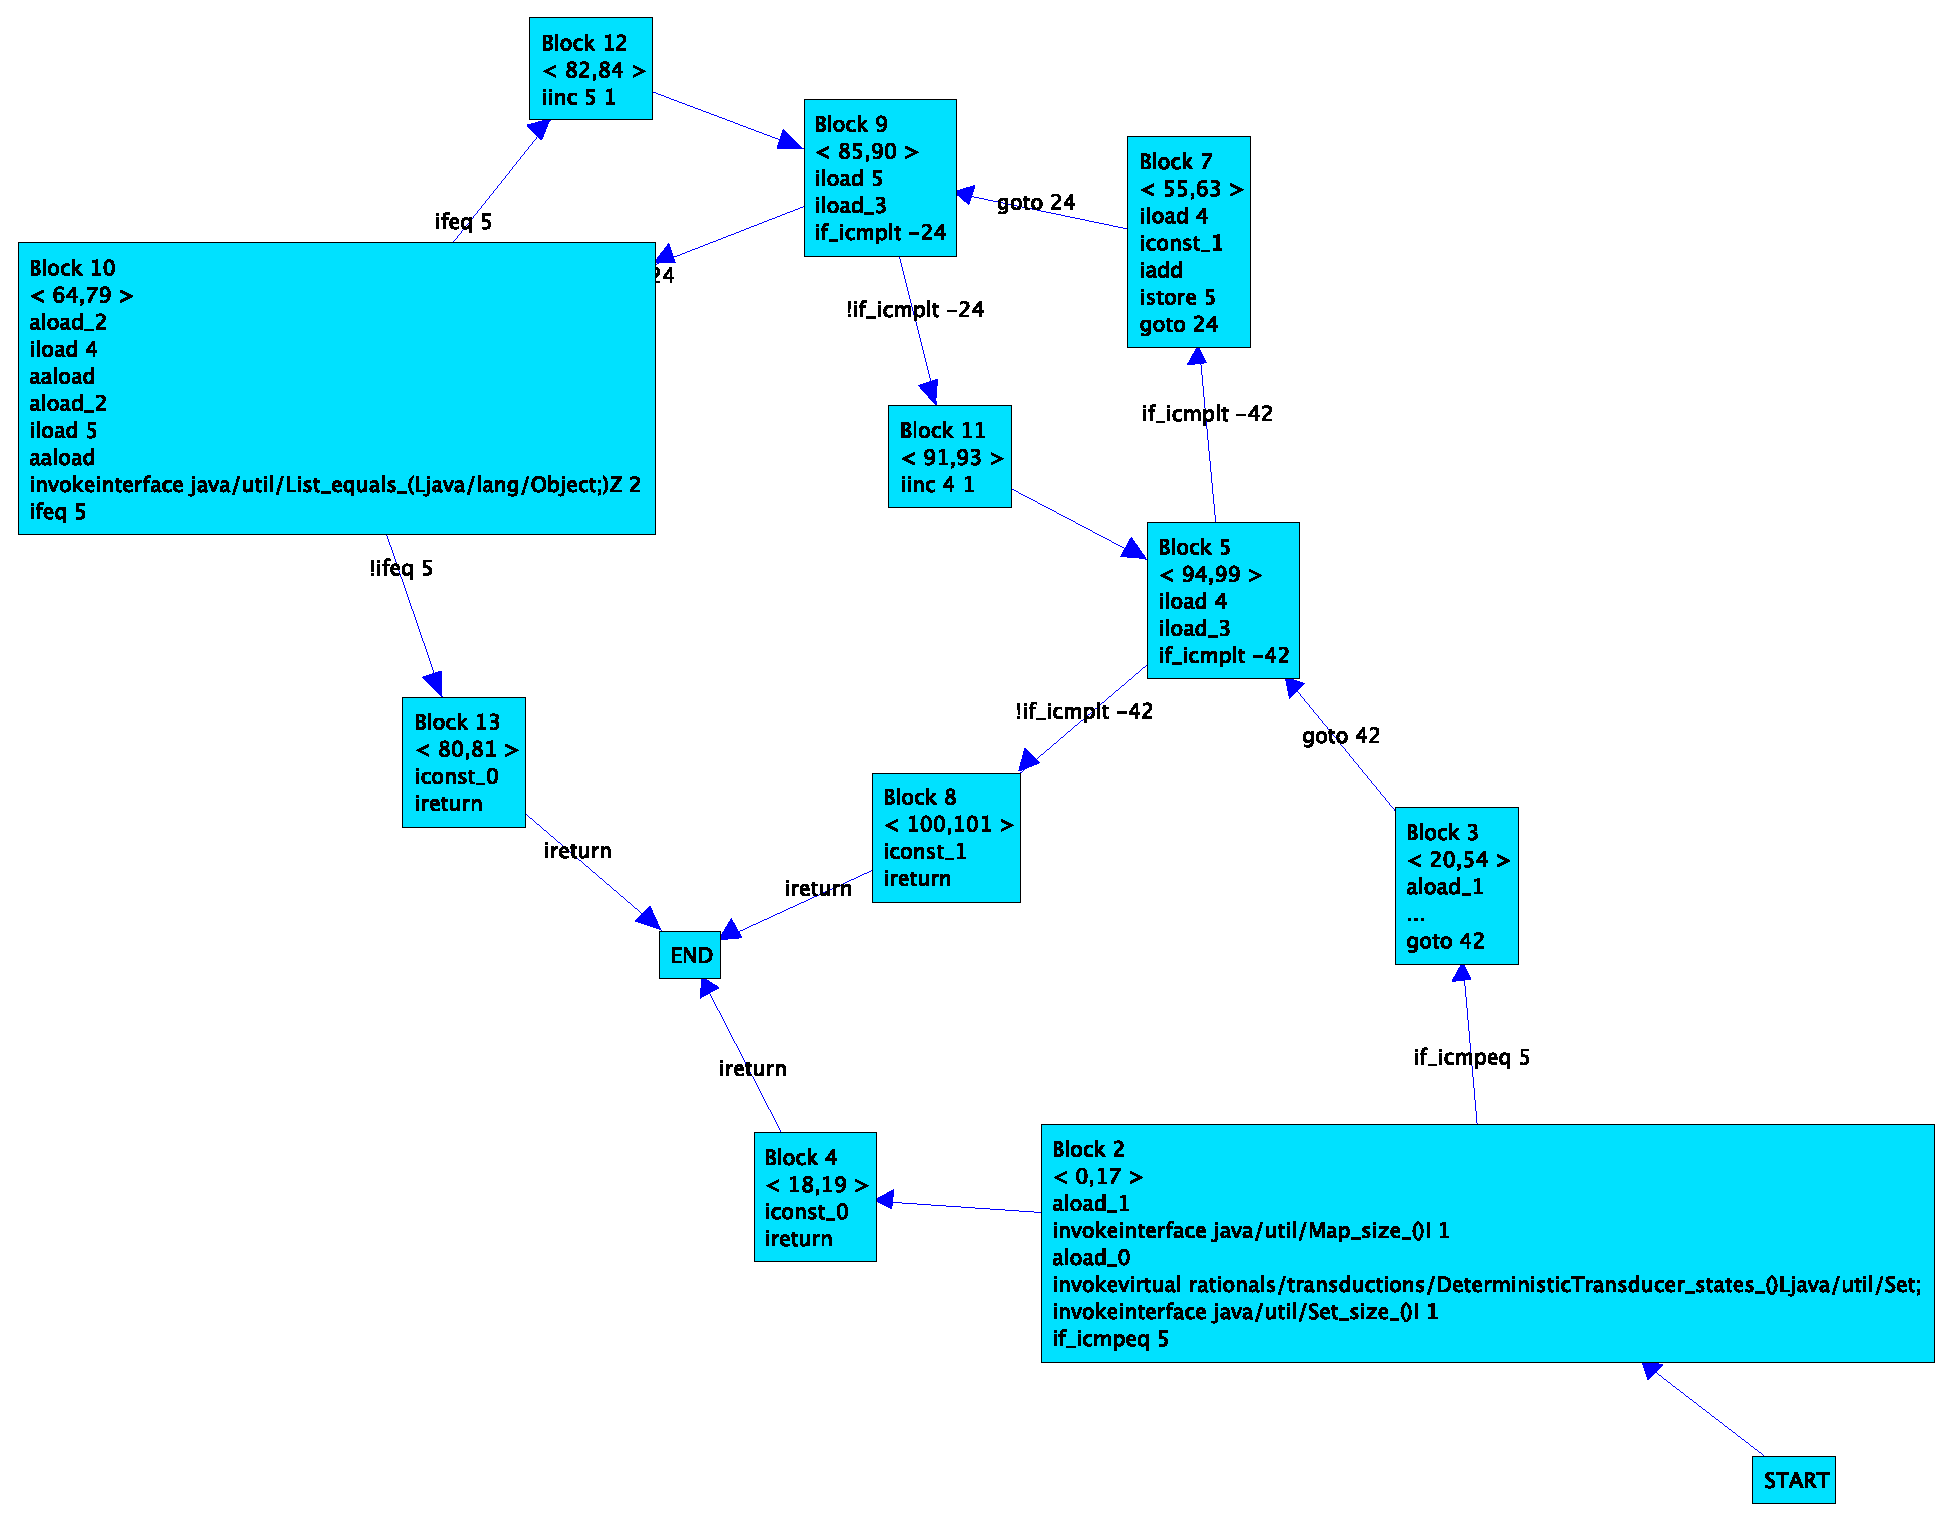
\includegraphics[width=\textwidth]{figures/fig-sample-control.eps}
    \caption{Exemple de graphe de contr\^ole}
    \label{fig-sample-control}
\end{figure}

\`A partir du graphe pr\'esent\'e, on peut donc d\'efinir en
fonction de diff\'erents crit\`eres de couvertures des
suites de tests qui sont des ensembles de chemins dans le
graphe de contr\^ole. Il restera pour chacune de ces s\'equences
\`a d\'efinir les valeurs de variables permettant de r\'ealiser
effectivement la s\'equence choisi, ce qui est un probl\`eme souvent
ardu. 

Par exemple, l'ensemble $\{(2,3,5,7,9,11,5,7,9,10,12,9,10,13), (2,4),
(2,3,5,8)\}$ est potentiellement ad\'equat pour les crit\`eres \emph{tous-les-n\oe uds} et
\emph{tous-les-arcs} du graphe de contr\^ole de  la figure
\ref{fig-source-sample-control}. Il reste \`a montrer qu'un certain
ensemble des valeurs des variables d'entr\'ee permet de sensibiliser
ces chemins.

Les crit\`eres bas\'es sur le flot de donn\'ees s'int\'eressent
\`a la couverture des relations entre la d\'efinition d'une
variable et son utilisation. Une hi\'erarchie de 
crit\`eres bas\'ee sur la notion de chemin \emph{def-use} est aussi construite. La figure
\ref{fig-sample-data} est une repr\'esentation d'un graphe de
flot de donn\'ees simplifi\'e pour le graphe de contr\^ole
\ref{fig-sample-control}. Les n\oe uds sont des utilisations ou des
d\'efinitions de variables --- marqu\'ees \textsf{Use i} ou
\textsf{Def i} --- et les arcs sont une extension des arcs du graphe
de contr\^ole permettant de relier chaque n\oe ud. 

Nous n'avons pas ici distingu\'e les n\oe uds de type
\emph{p-use} --- utilisation d'une variable pour un pr\'edicat de
branchement conditionnel --- des n\oe uds \emph{c-use} --- utilisation
pour une instruction, un appel .... \cite{vincenzi-covtest-java} est une proposition d'outil et de
m\'ethode pour le test de couverture de fl\^ot de contr\^ole et de
donn\'ees pour programmes \textsf{Java}. Comme dans les exemples
pr\'esent\'es figures \ref{fig-sample-control} et
\ref{fig-sample-data}, le principe est d'extraire ces graphes du
\emph{code-octet} repr\'esentant un programme \textsf{Java}.

\begin{figure}[htbp]
    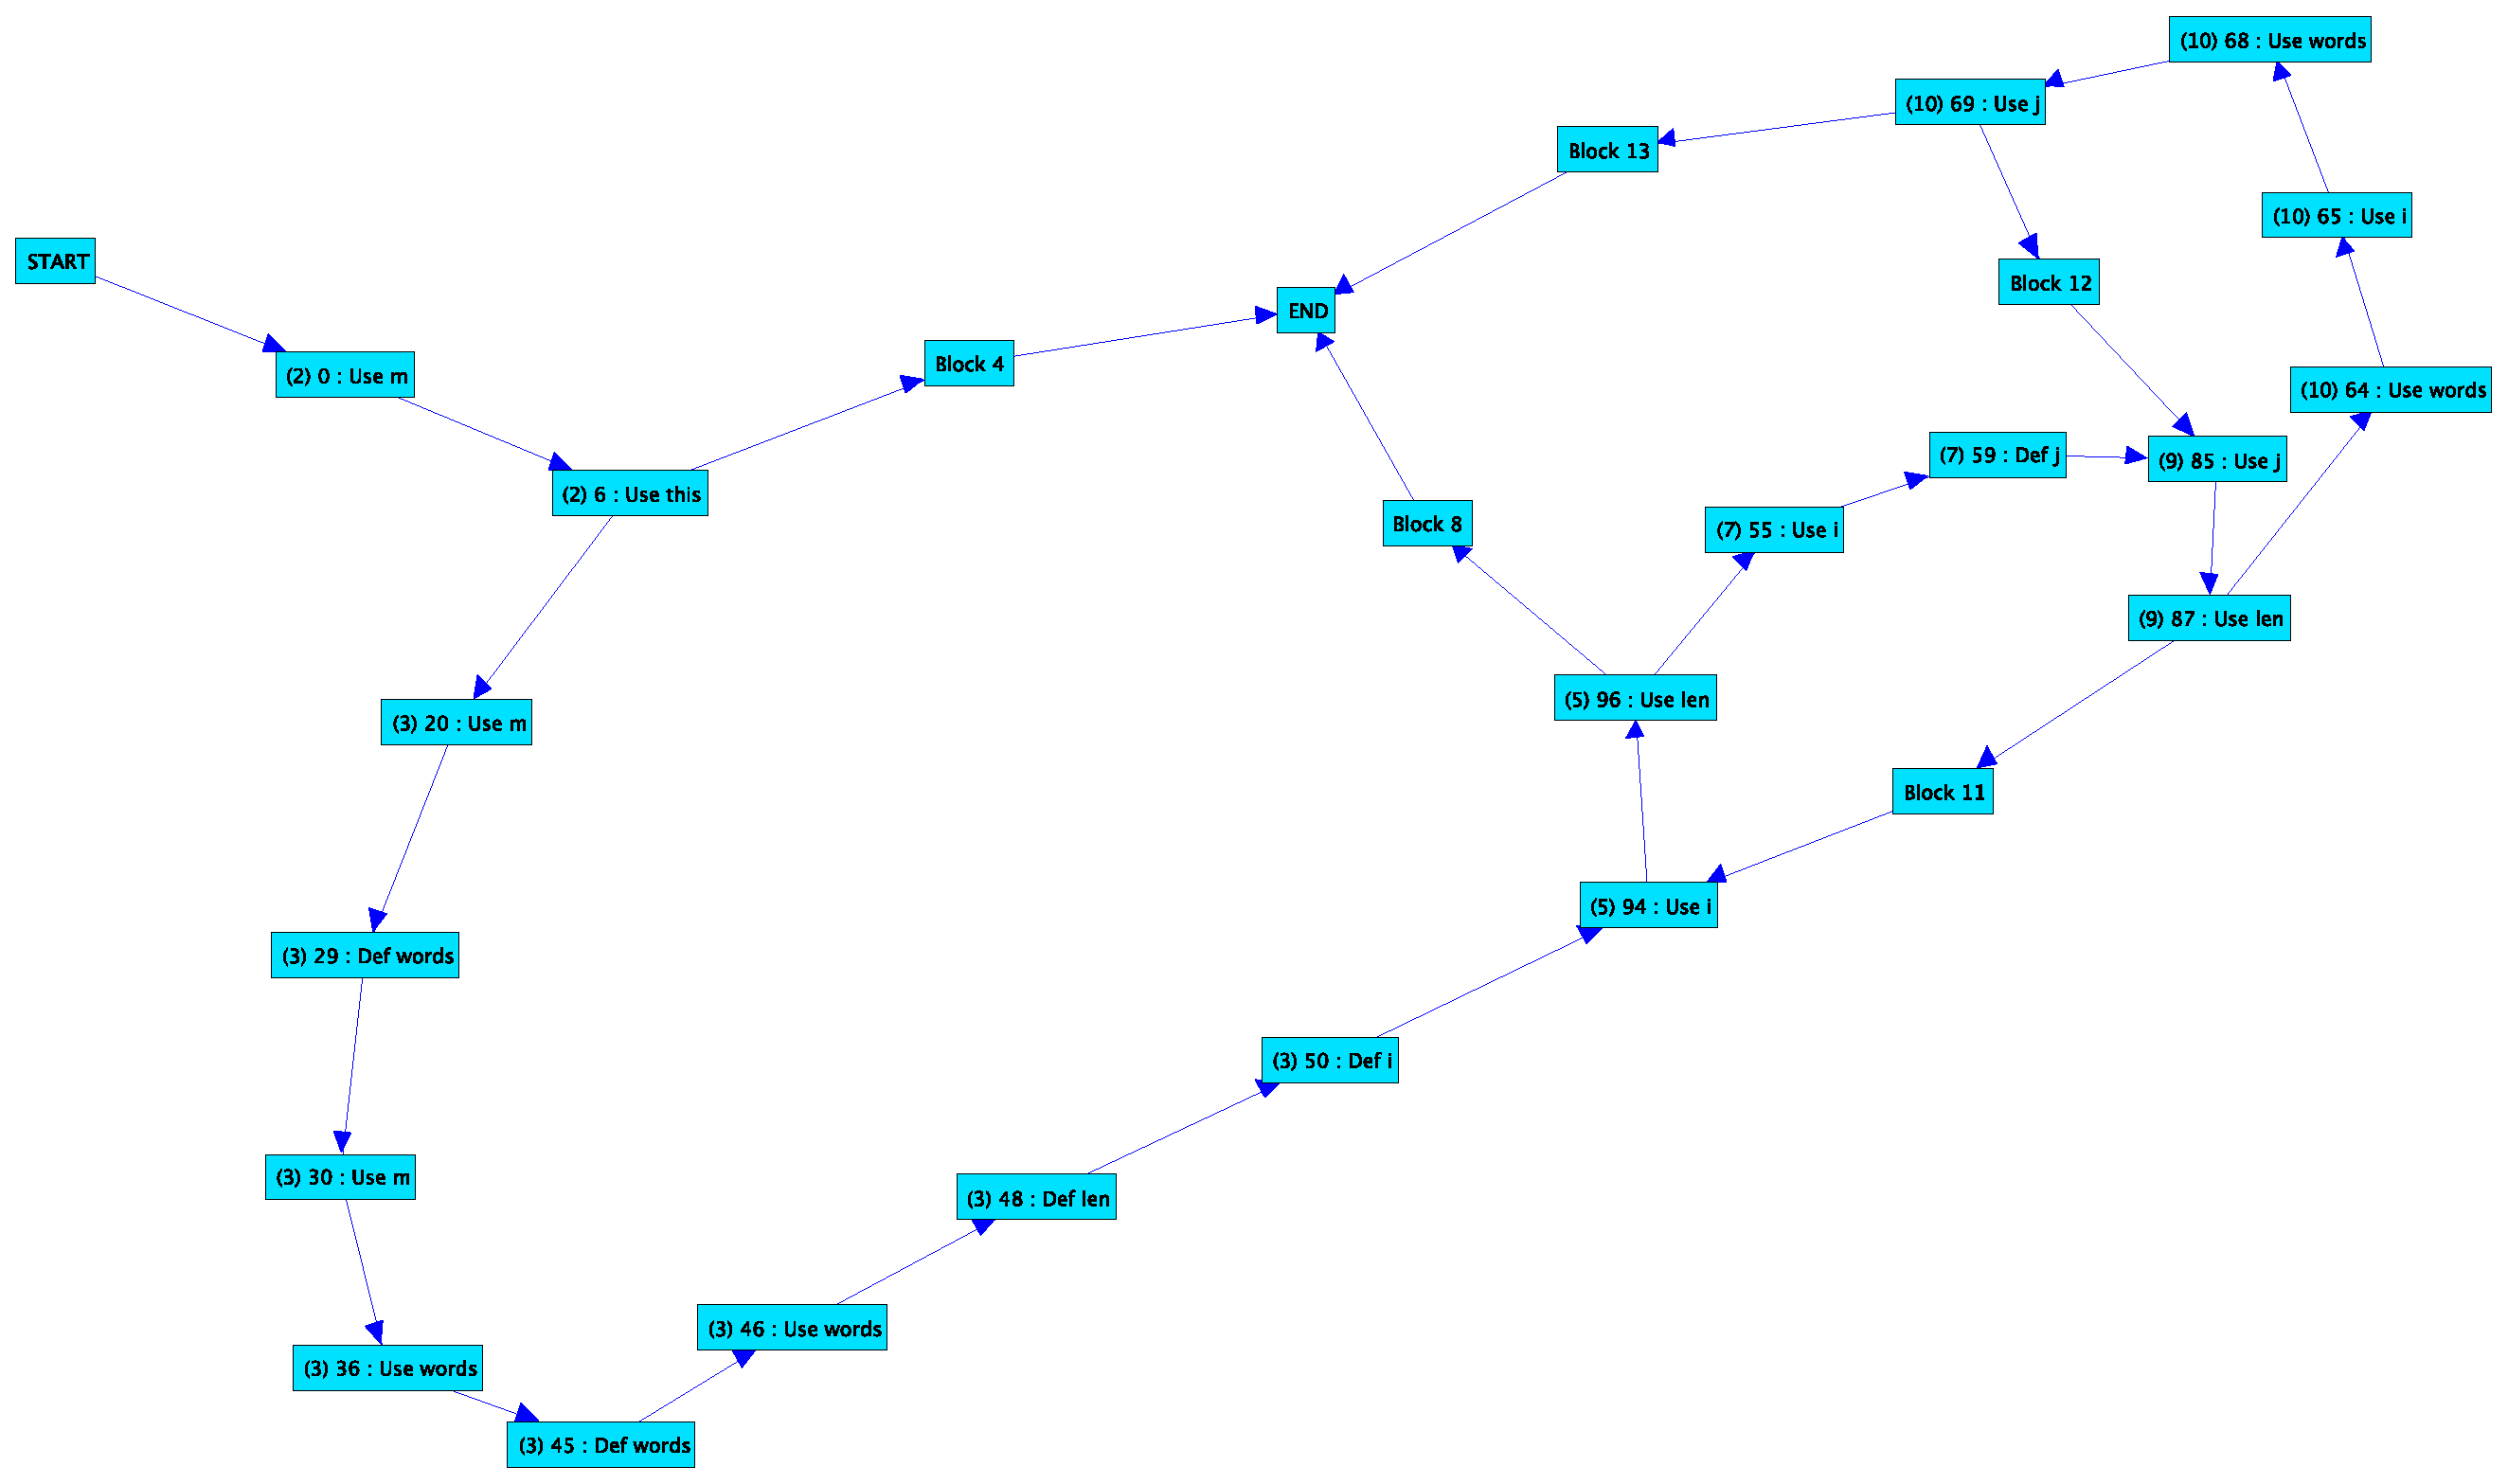
\includegraphics[width=\textwidth]{figures/fig-sample-data.eps}
    \caption{Exemple de graphe de flot de donn\'ees}
    \label{fig-sample-data}
\end{figure}

Le probl\`eme principal li\'e \`a l'utilisation de crit\`eres de
ce genre consiste bien \'evidemment \`a construire un jeu de tests
permettant de respecter le crit\`ere ce qui n'est pas toujours
possible et est m\^eme ind\'ecidable dans le cas g\'en\'eral.
La figure \ref{fig-hierarchie-couv} pr\'esente une vue partielle de
cette hi\'erarchie des crit\`eres de test pour quelques crit\`eres courants.

\begin{figure}[htbp]
    \centering
    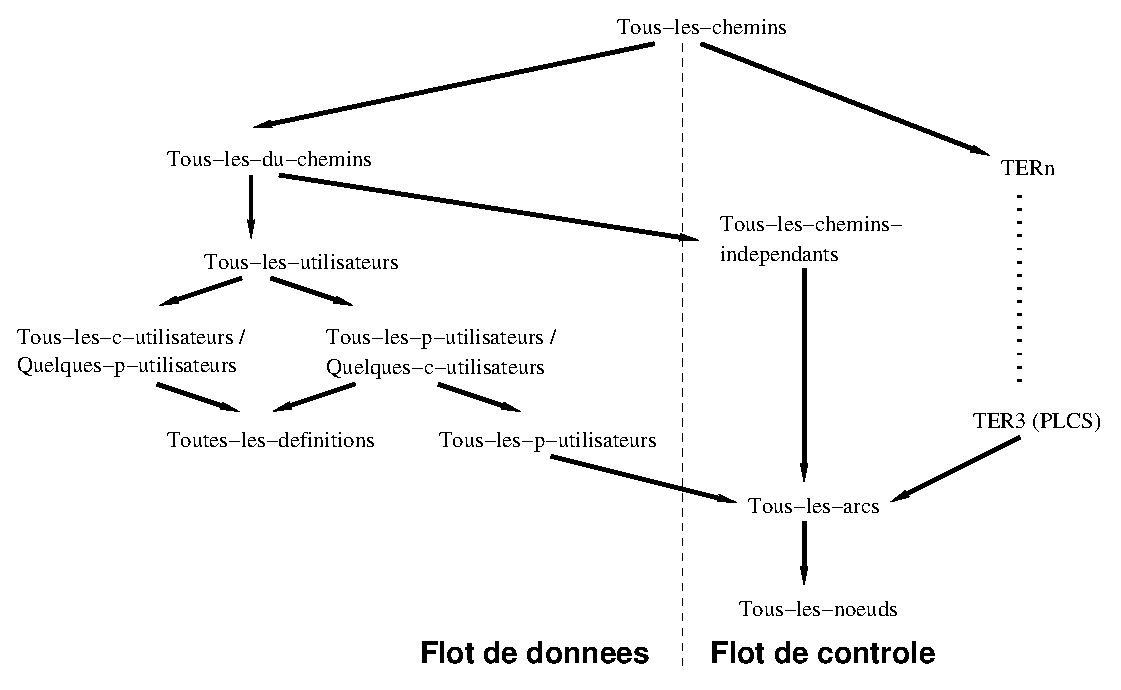
\includegraphics[width=\textwidth] {figures/hiertest.eps}
    \caption{Hi\'erarchie usuelle des crit\`eres de couverture}
    \label{fig-hierarchie-couv}
\end{figure}

Ce  probl\`eme  de \emph{sensibilisation} des chemins d'ex\'ecution
possible du programme a \'et\'e d\'ej\`a abord\'e dans
\cite{boyer-select} comme une forme d\'eriv\'ee de la preuve
automatique de th\'eor\`eme. Le principe de \texttt{SELECT} est de
r\'ealiser une ex\'ecution symbolique du programme test\'e pour
construire des ensembles des chemins d'ex\'ecution ayant la forme de
pr\'edicats sur les variables du programme. Les syst\`emes de
contraintes ainsi construits sont ensuite r\'esolus pour fournir des
valeurs d'entr\'ee permettant de sensibiliser chaque chemin. Ce
principe a \'et\'e repris dans \cite{gotlieb-clp-test} et dans
l'outil \textsf{InKa} d\'eriv\'e de ces travaux, en utilisant en syst\`eme
de r\'esolution de contraintes.

On peut aussi utiliser d'autres solutions algorithmiques pour
rechercher des valeurs permettant de sensibiliser un chemin
particulier comme par exemple l'algorithme g\'en\'etique de
\cite{testgenetic} : un vecteur de valeurs d'entr\'ee est
optimis\'e en fonction d'un objectif --- chemin ou \'etat --- et du
nombre de pr\'edicats que le vecteur de valeurs permet de satisfaire
--- fonction de \emph{fitness}.  \cite{tdgen-survey} est une \'etude
des diff\'erentes techniques de recherche heuristiques utilis\'ees
pour la d\'ecouverte de donn\'ees permettant de sensibiliser des
chemins dans un graphe de contr\^ole.

\subsubsection{Analyse de domaine}

Pour s\'electionner les cas de tests, on peut aussi s'int\'eresser
aux caract\'eristiques de l'espace d'entr\'ee ou de sortie du
programme et d\'efinir un objectif en fonction de celui-ci et d'une
\emph{partition}  du domaine en sous-domaines permettant de
sensibiliser tel ou tel chemin ou de valider tel crit\`ere. Une tactique usuelle consiste \`a s'int\'eresser
aux valeurs limites de chaque sous-domaine, sous l'hypoth\`ese que ce
sont ces valeurs qui seront le plus pathog\`enes. Dans le cas des
domaines num\'eriques entiers,  cette strat\'egie permet
classiquement de d\'etecter des erreurs d'utilisation de relations
entre valeurs, un $\leq$ se transformant par exemple en un
$<$. \cite{kosmatov-boundary-issre04} pr\'esente une formalisation de
ce crit\`ere au cas de sp\'ecifications formelles de type \textsf{Z}
ou \textsf{B}. Les partitions de domaines sont d\'eduites des
pr\'edicats sur les variables de la sp\'ecification et r\'esolues
par approximation dans un domaine continu --- par exemple les r\'eels
--- puis retransform\'ees dans le domaine --- discret
d'origine. 
La notion de partitionnement de domaine est aussi sous-jacente dans
les hypoth\`eses de r\'egularit\'e et d'uniformit\'e introduites
dans \cite{gaudel}.

\subsection{S\'election statistique \& al\'eatoire}

Dans la premi\`ere partie de ce chapitre, nous avons introduit la
notion de \emph{profil op\'erationnel} comme un outil d'aide \`a la
s\'election des tests dans le test dit syst\`eme. Un profil
op\'erationnel est simplement une distribution probabiliste de
l'espace d'entr\'ee de l'\textsf{IUT}. Une tactique de test \'evidente
consiste donc \`a \'echantillonner cette espace d'entr\'ee pour
l'utiliser comme donn\'ee de test et \`a
induire des lois  statistiques une fiabilit\'e du logiciel en
fonction des r\'esultats du test. \cite{thprobtest} propose de formaliser le test
probabiliste fonctionnel, de mani\`ere similaire \`a
l'ing\'enierie de la fiabilit\'e, en calculant \`a partir d'un
\'echantillonage des valeurs de l'espace d'entr\'ee une
probabilit\'e de correction --- pour des tests r\'eussis --- en
fonction d'une marge d'erreur et d'un intervalle de confiance. 

\cite{thevenod-stat-test} d\'efinit une notion de qualit\'e de
test en fonction d'un crit\`ere de test et de la taille de la suite
de tests s\'electionn\'ee par \'echantillonage sur une distribution
de l'espace d'entr\'ee construite en fonction du crit\`ere de
couverture \`a atteindre. Il ne s'agit plus ici d'un
profil op\'erationnel correspondant \`a un usage attendu de l'IUT
mais d'un \emph{profil de test} sp\'ecifiquement construit en
fonction d'un objectif pr\'ed\'efini et permettant d'\'evaluer la
qualit\'e du r\'esultat produit de mani\`ere statistique. Bien
s\^ur, la fiabilit\'e globale du test r\'ealis\'e reste
d\'ependante de la confiance que l'on place dans le crit\`ere choisi,
avec cette diff\'erence par rapport au cas d\'eterministe que les
cas de tests sont s\'electionn\'es al\'eatoirement et donc sans
le biais  d'une s\'election arbitraire. Cette technique est
d\'evelopp\'ee dans \cite{gouraud-issre04}, en utilisant des
techniques de g\'en\'eration al\'eatoire de structures
combinatoires, pour le test statistique bas\'e sur des
sp\'ecifications prenant la forme de graphes.

Lorsque la distribution est uniforme, on a alors un \emph{test
  al\'eatoire}. \cite{thevenod-structtest,ntafos-comparison} montrent
exp\'erimentalement qu'il n'est pas forc\'ement l'approche la moins efficace pour la
d\'etection des erreurs.

\subsection{Test mutationnel}

Le test mutationnel --- \emph{mutation testing} en anglais ---
constitue une
technique indirecte pour s\'electionner une suite de test pertinente.
Cette technique a \'et\'e introduite dans
\cite{demillo-mutation}. Son principe est d'\'evaluer la
fiabilit\'e de la suite de test par rapport \`a un \emph{mod\`ele
  de faute} : 
\begin{itemize}
  \item on d\'efinit pour un langage ou un format binaire donn\'e un
    ensemble d'\emph{op\'erateurs de mutations} atomiques : inversion
    de relations binaires, changements de variables, transformations
    d'op\'erateurs arithm\'etiques, modifications de constantes en
    variables, ... Ces op\'erateurs de mutation repr\'esentent  des
    erreurs courantes que peut introduire un \emph{programmeur
      comp\'etent} dans un logiciel et constituent donc un mod\`ele
    des fautes que la suite de test va rechercher ;
  \item on applique ces op\'erateurs de mani\`ere \og
    syst\'ematique~\fg sur le logiciel test\'e produisant ainsi des
    \emph{mutants}, c'est \`a dire des versions proches du logiciel
    original mais g\'en\'eralement incorrectes. Chaque mutant diverge de son parent par
    une seule op\'eration de mutation selon le principe du couplage
    des erreurs : une suite de test r\'ev\'elant des erreurs simples
    sera capable de r\'ev\'eler des erreurs complexes. Autrement
    dit, les erreurs complexes sont issues de plusieurs erreurs simples
    (voir \cite{offutt-coupling} pour une discussion exp\'erimentale de
    la question). Le probl\`eme des mutants \'equivalents  est loin d'\^etre trivial mais
    est n\'eglig\'e en pratique ;
  \item on \'ecrit ou enrichit une suite de tests \emph{tuant}
    le maximum de mutant, c'est \`a dire que lorsqu'elle est
    ex\'ecut\'ee sur les mutants, elle r\'ev\`ele qu'ils sont
    incorrects en produisant \'echec du test ;
\item le \emph{score de mutation} de la suite de tests est \'egal au
  nombre de mutants tu\'es sur le nombre total de mutants non-\'equivalents.
\end{itemize}
Ce score de mutation est une mesure de la qualit\'e de la suite de
tests et donc de la qualit\'e du logiciel : si le logiciel  passe la
suite de tests dont le score de mutation est \'elev\'e, c'est donc
qu'il ne contient pas les fautes inject\'ees par le test de
mutation. Implicitement, cette m\'ethode se base sur deux
hypoth\`eses :
\begin{description}
  \item[Hypoth\`ese du programmeur comp\'etent] : le logiciel
  test\'e est \emph{a priori} presque correct et les erreurs de
  programmation sont simples ;
\item[Hypoth\`ese du couplage] : les erreurs complexes sont des
  suites d'erreurs simples.
\end{description}

On voit bien que la fiabilit\'e de cette approche  d\'epend du choix
des op\'erateurs de mutation et de leur ad\'equation avec les erreurs
susceptibles de se produire r\'eellement, ainsi que du nombre et de
la r\'epartition des mutants g\'en\'er\'es. Ce dernier point la
rend d'ailleurs tr\`es co\^uteuse en temps d'ex\'ecution et de
r\'ealisation des tests. Dans \cite{these-baudry}, cette approche est
utilis\'ee coupl\'ee avec un algorithme g\'en\'etique pour
optimiser des suites de tests.

Le test mutationnel a une litt\'erature relativement abondante et a
donn\'e lieu \`a la cr\'eation d'une faune vari\'ee
d'op\'erateurs de mutations, en particulier dans le cadre des
langages \`a objets. Cette technique est tr\`es
utilis\'ee pour comparer des  m\'ethodes de s\'election de cas de
test entre elles. 

\section{Discussion}

On a vu que le test logiciel, m\^eme restreint au seul cas du test de
syst\`emes \`a \'etats-transitions, offre un champ
extr\^emement vaste de travaux qui se sont toutefois essentiellement
concentr\'es dans deux directions : d'une part la s\'election
efficiente de suites de tests dans le cas des \textsf{FSM}, d'autre part la
d\'efinition de relations de conformit\'e pertinentes dans le
domaine des \textsf{IOLTS}. 

Nous avons aussi vu que le probl\`eme de la s\'election des cas de
test se ramenait essentiellement au probl\`eme de la d\'efinition
d'un \emph{objectif de test}, au sens large du terme, d\'ependant des
artefacts \`a la disposition du testeur, et qu'il existait un nombre
tr\`es importants de crit\`eres heuristiques difficilement
comparables entre eux.

\subsection{Test bas\'e sur les mod\`eles}

Nous nous sommes concentr\'es dans l'exposition de cet \'etat de
l'art sur des m\'ethodes \emph{primitives} de test. Ces m\'ethodes
constituent la  base d'autres m\'ethodes utilisant des mod\`eles
de plus haut niveau tels que les diagrammes \textsf{UML} ou, plus
rarement, les \textsf{ADL}.

Il existe une litt\'erature importante consacr\'ee \`a
l'application de ces m\'ethodes au cas de diagrammes \textsf{UML} et
plus particuli\`erement des
Statecharts\cite{jezequel-msc-testd,umlaut,umlinttest,offutt,tdgen-state,testselectstatecharts,scollo-archi-test}.
La question de tests d'int\'egration et de leur ordonnancement \`a
partir de mod\`eles UML est abord\'ee dans \cite{umlinttest} et
\cite{jeron-integ-regr-ootest}. 
\cite{test-pf} est une approche bas\'ee sur les cas d'utilisation et
les contraintes associ\'ees. \`A partir d'un diagramme  de cas
d'utilisations enrichi de pr\'edicats et  de variables, et des
d\'ependances entre cas d'utilisations, on construit
un diagramme d'\'etats finis qui est inject\'e dans \textsf{TGV}
pour produire une suite de tests
syst\`emes. \cite{briand-uml-systesting} a une approche similaire
bas\'ee sur l'utilisation de contraintes \textsf{OCL}. 

\cite{muccini-archi-test} propose une m\'ethode d'extraction de cas
de tests unitaires \`a partir d'une description d'architecture dont
le comportement est mod\'elis\'e sous forme de \textsf{LTS}. Ce
travail est dans l'id\'ee proche de notre d\'emarche : il s'agit de
construire des tests de composants \`a partir d'une sp\'ecification
d'architecture. Dans le d\'etail, les m\'ethodes diff\`erent : le
test n'est pas ici conduit de mani\`ere syst\'ematique mais \`a
partir de la d\'efinition d'un \emph{objectif de test}, le crit\`ere
de s\'election choisi est bas\'e sur la complexit\'e de
\textsc{McCabe}\cite{mccabe-complexity-testing}, les tests abstraits d\'eriv\'es doivent \^etre
manuellement \og traduits\fg en tests ex\'ecutables en fonction du
composant test\'e. 
\cite{tool-ccm-test,ccmtesting} pr\'esentent une architecture et un
outil pour le test de composants \textsf{CCM}. La question du
probl\`eme de la s\'election des cas de tests n'est toutefois pas
abord\'ee. \cite{cavalli-corba-iscc} est une application aux objets
\textsf{CORBA} de l'algorithme \emph{Hit-Or-Jump} pr\'esent\'e \`a
la section \ref{sec:test-fsm-heuristic}. 

\subsection{Analyse}

\cite{lai-prototest-survey} souligne la distance qui
existe entre la foultitude de mod\`eles et d'algorithmes produits par
le monde universitaire et l'\'etat concret des pratiques dans
l'industrie :
\begin{quote}
    \og [...] this state-of-the-art research is not necessarily
    state-of-the-practice. Academic methods are seldom employed in
    industry. [...] There is not much progress in the use of test
    sequence generation techniques for practical testing of
    communication networks. \fg
\end{quote}
La port\'ee  de cette affirmation doit toutefois \^etre
mod\'er\'ee par le fait que l'auteur n'envisage qu'une classe de
syst\`emes de transitions dans son \'etude, les \textsf{FSM}. Il n'en reste
pas moins vrai que l'activit\'e du test dans le monde industriel est
encore largement \og manuelle\fg.
La situation est identique dans le monde des services logiciels comme on l'a vu au chapitre
\ref{cha:proc-de-devol}. 

Les notions d'\'equivalence dans les FSM et les IOLTS sont
fondamentalement diff\'erentes. Dans le premier cas, on a une
\'equivalence entre des \emph{fonctions} : le \textsf{FSM} est un
transducteur calculant une fonction \`a partir de param\`etres
d'entr\'ee. Le but du test de conformit\'e de \textsf{FSM} est de
v\'erifier ce calcul en parcourant l'espace des valeurs du
param\`etre d'entr\'ee qui est ici un \emph{langage}. Dans le second
cas, on v\'erifie une \'equivalence entre des \emph{langages}. Les
suite de tests ont donc des statuts et des structures diff\'erentes :
un ensemble de s\'equences d'entr\'ee d'une part, un ensemble de
mots du langage d'autre part. Et le processus de test est bien s\^ur
diff\'erent : sensibilisation du FSM d'une part, synchronisation des
deux langages d'autre part.

Le panorama que nous avons fait dans ce chapitre nous permet de mieux
nous orienter dans l'approche choisie. On voit clairement que notre
objectif est similaire \`a celui du test de conformit\'e
r\'eparti pour des syst\`emes de transitions \`a entr\'ee-sortie (section
\ref{sec:le-test-reparti}). Ces travaux s'appuient sur les relations de conformit\'e
d\'efinies \`a la section \ref{sec:test-de-lts}. Ces
relations,  et en particulier la relation
\textbf{ioco}, ne sont toutefois pas satisfaisantes dans notre
contexte : elles ne tiennent pas compte de
la nature \emph{contractuelle} des sp\'ecifications de composants que
nous utilisons ni de l'asym\'etrie existant dans les
composants entre les interfaces requises et les interfaces fournies. 
 
Par ailleurs, notre approche de la mod\'elisation des composants est fond\'ee sur les automates et
la th\'eorie des langages. Il est donc naturel que nous choisissions
d'exprimer la notion de conformit\'e en termes d'une relation
d'\'equivalence sur des langages et par cons\'equent que les tests
permettant de v\'erifier cette relation soient r\'ealis\'es sous la
forme d'un produit de synchronisation entre les langages.

%%% Local Variables: 
%%% mode: latex
%%% TeX-master: "these"
%%% End: 

\chapter{Mod\`ele de composants FIDL}
\label{chap-fidl}
\lstset{basicstyle=\footnotesize\sffamily,frame=single}

L'analyse des mod\`eles et outils existants
permettant de d\'efinir et r\'ealiser des architectures de
composants nous a permis d'une part de d\'egager les concepts
fondamentaux relatifs \`a ce domaine : composants, interfaces, ports
et connexions. D'autre part, nous avons constat\'e qu'il existait une certaine distance entre des mod\`eles
permettant de \emph{concevoir} et v\'erifier des propri\'et\'es sur
des architectures de composants, sch\'ematiquement les \emph{langages de
description d'architecture} formels, et d'autre part les plateformes
et implantations concr\`etes permettant de construire et ex\'ecuter
des syst\`emes de composants. Notre objectif est d'\^etre capable
non seulement de raisonner sur des mod\`eles mais aussi d'utiliser
ces sp\'ecifications pour \emph{v\'erifier} des implantations
concr\`etes de mod\`eles, en particulier par le test. Par ailleurs, on souhaite que ces
mod\`eles soient suffisamment abstraits de l'implantation pour \^etre
\emph{r\'eutilisables}, ce dans l'optique de construire une
d\'emarche formalis\'ee d'\emph{ing\'enierie dirig\'ee par les
mod\`eles}. Le but final est bien entendu de d\'ecoupler la
mod\'elisation des processus m\'etiers de la conception des
syst\`emes les r\'ealisant.

Dans ce chapitre, nous pr\'esentons en d\'etail mais de mani\`ere
informelle un \emph{mod\`ele de
composants abstraits} nomm\'e \textsf{FIDL} pour \emph{Formal Interface
Definition Language}. La premi\`ere partie de ce chapitre est 
une exposition informelle des principaux \'el\'ements de ce
mod\`ele qui reprend les concepts
fondamentaux d\'egag\'es au chapitre pr\'ec\'edent --- composants,
interfaces, ports, connecteurs, assemblages --- et y int\`egre une
description du comportement des diff\'erents \'el\'ements. Ce mod\`ele est concr\'etis\'e au travers
d'un langage dont nous pr\'esentons la syntaxe \`a la section
\ref{sec:syntaxe-fidl}. La s\'emantique de ce langage est d\'efinie
en termes d'ensembles de traces, des langages clos par
pr\'efixes, correspondant au langage accept\'e par une certaine
forme d'automates appel\'ee automates \textsf{FIDL}. Ces
aspects seront d\'ecrits plus formellement aux chapitres
\ref{cha:automates-fidl} et \ref{cha:composition} et nous nous
contenterons dans le pr\'esent chapitre d'utiliser  ce formalisme de
mani\`ere intuitive. Nous illustrerons
cette pr\'esentation par quelques exemples 
significatifs de mod\'elisation de probl\`emes concrets.

\section{G\'en\'eralit\'es}

Un composant est une \emph{unit\'e architecturale}
communiquant avec son environnement au travers de \emph{ports}
(\emph{cf.} \cite{compsoft}). Un syst\`eme est constitu\'e par
l'interconnexion d'un ensemble de ports de composants compatibles. Un composant est consid\'er\'e comme une \emph{bo\^{\i}te
  noire} dont l'\'etat interne ne peut \^etre observ\'e qu'au travers des
messages \'echang\'es avec les autres composants. Autrement dit, nous ne
faisons aucune hypoth\`ese dans le mod\`ele sur les modalit\'es d'ex\'ecution
des \'el\'ements du syst\`eme. 

Les composants fournissent et utilisent des \emph{services} au travers
des ports synchrones typ\'es par interfaces. Les interfaces fournies
sont appel\'ees \emph{facettes}, celles utilis\'ees sont appel\'ees
\emph{r\'eceptacles}. Les composants peuvent \'egalement communiquer en
utilisant des \emph{\'ev\'enements asynchrones}, les \emph{sources d'\'ev\'enements} sont des ports utilis\'es 
pour \'emettre des \'ev\'enements, les \emph{puits d'\'ev\'enements} sont les
ports par lesquels les composants re\c{c}oivent les \'ev\'enements
asynchrones  et chaque port d'\'ev\'enement asynchrone d\'efinit le
type --- la structure --- des \'ev\'enements susceptibles de
transiter par ce port. Nous utiliserons le terme de \emph{message}
pour d\'esigner collectivement toutes les occurrences
d'\'ev\'enements asynchrones, d'appels, de retours ou d'exceptions
de m\'ethodes.
Le sch\'ema \ref{fig-composant} est la repr\'esentation d'un
composant introduite dans  \cite{cesure} et tr\`es proche de
celle utilis\'ee dans le \textsf{CCM}. 

\begin{figure}[htbp] 
    \begin{center} 
        \epsfig{figure=figures/composant.eps,width=8cm}
    \caption{Composant.}
        \label{fig-composant}
\end{center} 
\end{figure} 

Le sch\'ema \ref{fig-mmcomposants} est un mod\`ele \textsf{UML}
d\'ecrivant le mod\`ele de composants \textsf{FIDL}, autrement dit
un \emph{m\'eta-mod\`ele de composants}. On constatera que ce
mod\`ele est proche du mod\`ele de base du
\textsf{CCM} (voir figure \ref{fig-ccm-model}, page
\pageref{fig-ccm-model}) et qu'il
n'inclut pas d'\'el\'ements relatifs \`a la gestion du cycle de vie
des composants qui est explicitement hors du cadre de ce travail. 

L'utilit\'e de ce m\'eta-mod\`ele appara\^{\i}tra
au chapitre~\ref{cha:methodes--outils} lorsque nous \'etudierons
concr\`etement comment le mod\`ele \textsf{FIDL} peut \^etre utilis\'e dans la
plate-forme du m\^eme nom pour tester des composants concrets issus
de diff\'erentes technologies.

\begin{figure}[htbp]
    \centering
    \includegraphics[angle=-90,width=\textwidth]{figures/fig-mmcomposant.eps}
    \caption{M\'eta-mod\`ele de composants \textsf{FIDL}}
    \label{fig-mmcomposants}
\end{figure}


\subsection{Interfaces \& ports synchrones}

Une interface \textsf{FIDL} d\'efinit un \emph{protocole} de communication entre deux
composants au travers d'une \emph{connexion}, protocole d\'efini sous la forme d'\emph{op\'erations}  --- ou
m\'ethodes --- et d'\emph{attributs} susceptibles de g\'en\'erer des
appels, des retours et des exceptions. Une op\'eration est identifi\'ee
par son nom, le type et la modalit\'e ---  \texttt{in},
\texttt{inout} et \texttt{out} --- de ses param\`etres. 
Le cas des attributs est un cas particulier : ils ne sont accessibles que
par l'interm\'ediaire d'\emph{accesseurs} et de \emph{mutateurs}, c'est
\`a dire des op\'erations implicites nomm\'ees \texttt{getXXX} et
\texttt{setXXX} respectivement pour chaque attribut \texttt{XXX}. 

Une interface peut h\'eriter d'une ou plusieurs autres interfaces ce qui
ne pose pas de probl\`emes de r\'esolution statique : l'absence de corps
de m\'ethode n'introduit pas les conflits d'h\'eritages typiques des
langages \`a h\'eritage multiple tels que le \textsf{C++}. L'h\'eritage pose
toutefois un certain nombre de probl\`emes lorsque l'on prend en compte
la sp\'ecification formelle des interfaces et cette question sera
\'etudi\'ee dans la section \ref{sec:heritage-comportemental} du chapitre \ref{cha:composition}.

Une interface d\'efinit le \emph{type} d'une facette ou d'un
r\'eceptacle susceptibles d'\^etre d\'eclar\'es dans la
d\'efinition d'un composant. Ce type est un \'el\'ement permettant de
v\'erifier la validit\'e d'une connexion entre facette et r\'eceptacle : la
facette doit \^etre un sous-type du type du r\'eceptacle pour que la
connexion soit, au moins syntaxiquement, consid\'er\'ee comme l\'egale. 

Enfin, il est possible de d\'efinir des modalit\'es de connexion pour
chaque facette :
\begin{itemize}
\item \emph{unique} si le port ne peut \^etre utilis\'e que par un et un
  seul composant \`a la fois  (c'est le cas par d\'efaut) ;
  \item \emph{single} si le m\^eme port peut \^etre partag\'e par
  plusieurs composants connect\'es ;
\item \emph{multiple} si chaque composant connect\'e \`a ce port est
  \emph{isol\'e} des autres composants. Le port est en fait multiplex\'e
  et chaque connexion poss\`ede son propre \'etat conversationnel
  ind\'ependant de toutes les autres connexions.
\end{itemize}

Cette notion de \emph{modalit\'e} d'interface permet d'int\'egrer dans la
sp\'ecification les typologies de mod\`ele d'ex\'ecution du
composant qui sont pr\'ecis\'ees dans le cas du \textsf{CCM} et
de \textsf{J2EE} par des descriptions externes. On dispose ainsi
des notions famili\`eres d'objet \emph{session}, \emph{processus} ou
\emph{m\'ethode}, transpos\'ees des composants \`a  leurs ports et
disponibles dans le mod\`ele, et un m\^eme composant pourra donc offrir
simultan\'ement des facettes de diff\'erentes modalit\'es. Par la
suite, nous consid\'ererons uniquement le cas des facettes
\emph{unique}. Le cas des facettes \emph{single} introduit le partage de facettes entre
plusieurs composants et ruine la possibilit\'e de composer les
composants en ne tenant compte que de leur \emph{topologie de connexion}, il 
impose donc pour valider une architecture de v\'erifier le respect des
contrats en fonction de l'ensemble des composants connect\'es et ne
permet pas de raisonner uniquement de mani\`ere
compositionnelle. C'est une version du probl\`eme bien connu  
de l'\emph{aliasing}. En ce qui concerne les facettes \emph{multiple},
leur traitement n'introduit pas de difficult\'e conceptuelle
suppl\'ementaire mais est techniquement assez complexe : compte tenu
du fait que le syst\`eme que nous d\'ecrivons et la s\'emantique
des langages de traces est d\'ej\`a relativement touffue, nous avons
choisi de reporter le traitement de ce cas \`a des travaux ult\'erieurs.

\subsection{\'Ev\'enements \& ports asynchrones}

Les ports d'\'ev\'enements asynchrones, \emph{sources} et \emph{puits} sont
typ\'es par le type d'\'ev\'enement --- un objet-valeur --- qu'ils sont
susceptibles de consommer ou de produire. Ces objets-valeur --- ou
\texttt{eventtype} --- sont des structures de donn\'ees arbitrairement
complexes. En \textsf{IDL3}, un \texttt{eventtype} 
peut d\'efinir des attributs, des op\'erations, des types export\'es,
etc... comme n'importe quel autre espace de nommage. C'est en fait un
v\'eritable \emph{objet}, au sens des langages objets, dont l'\'etat
peut-\^etre observ\'e et \'eventuellement modifi\'e par n'importe quel
\'el\'ement du syst\`eme. 

Dans un premier temps, nous ne nous int\'eresserons aux \'ev\'enements que
sous l'angle d'une structure de donn\'ees particuli\`ere transport\'ee par des
ports asynchrones. 

\subsection{Connexion \& composition}

Un composant ne peut \^etre fonctionnel que si tous ses r\'eceptacles sont
correctement connect\'es \`a une facette, et si toutes ses sources 
d'\'ev\'enements sont connect\'ees \`a un puits
d'\'ev\'enements. Les services synchrones et asynchrones requis par
le composant sont en effet suppos\'es \^etre utilis\'es par
celui-ci \`a un moment ou un autre pour qu'il soit en mesure de
rendre les services qu'il fournit. Une connexion
est une relation un-vers-un  entre ports de composants. 

Un \emph{composite} est un ensemble de composants  partiellement ou
totalement inter-connect\'es, autrement dit un composant r\'ealis\'e par
\emph{assemblage} de plusieurs autres composants. Nous utiliserons le
terme de Un \emph{syst\`eme} pour d\'esigner un ensemble quelconque
de ports sans identit\'e pr\'ecise. 

Du point de vue de la sp\'ecification, un composite peut permettre de
masquer certaines facettes et a pour effet principal de rendre
inobservable l'ensemble des messages transitant par les connexions
r\'ealis\'es entre ses composants.  
On notera que la notion de composite, conceptuellement simple et
  \'el\'egante, n'est pas aujourd'hui prise en compte 
  directement dans les plate-formes existantes, \`a l'exception de
  \textsf{.Net} sous la forme des \emph{assembly}. Elle est par contre essentielle dans
la plupart des mod\`eles formels \'etudi\'es. 

Les connexions sont r\'ealis\'ees durant la phase de d\'eploiement et peuvent normalement
\'evoluer au court du cycle de vie du composant. Nous
consid\'erons ici le cas simple o\`u les connexions des composants sont
  \'etablies au \emph{d\'eploiement} et ne sont plus modifi\'ees jusqu'\`a l'arr\^et du
  syst\`eme. 

\subsection{Ex\'ecution \& Communication}

Ainsi que nous l'avons dit pr\'ec\'edemment, aucune hypoth\`ese n'est faite
quant aux flots d'ex\'ecution des composants. Nous nous int\'eressons
uniquement aux messages \'echang\'es entre les diff\'erents composants au
travers de leurs connexions. Ces messages sont nomm\'es et contiennent
des donn\'ees primitives ou structur\'ees selon le typage des interfaces
du port concern\'e. De plus, ces messages identifient de mani\`ere
unique l'\'emetteur et  le r\'ecepteur.

Le m\'edium de communication est suppos\'e fiable : tous les messages
envoy\'es atteignent leur destination en un temps fini, mais nous ne
supposons rien quant \`a l'ordre d'arriv\'ee des messages entre
diff\'erentes connexions qui peuvent \^etre arbitrairement entrelac\'es. Sur une m\^eme connexion
point-\`a-point, l'ordre des messages est toutefois suppos\'e maintenu entre
l'\'emetteur et le r\'ecepteur. 

Les \'ev\'enements observables d'un syst\`eme sont les messages \'echang\'es
entre les composants de ce syst\`eme au travers de leurs connexions,
sachant que l'\'emission et la r\'eception d'un message constituent deux
\'ev\'enements distincts observ\'es \`a chacun des points de la
connexion. Chaque composant poss\`ede son propre point de vue sur le
syst\`eme et donc ne peut observer qu'un sous-ensemble des \'ev\'enements
globaux, en l'occurrence les messages re\c{c}us et \'emis sur les connexions
auxquelles il participe.

\section{Le langage \textsf{FIDL}}
\label{sec:syntaxe-fidl}
Le langage \textsf{FIDL} est  construit par agr\'egation de plusieurs langages,
chacun destin\'e \`a d\'efinir une partie du syst\`eme sp\'ecifi\'e :
\begin{enumerate}
  \item le langage \textsf{IDL3}, d\'efini dans le \textsf{CORBA Component
      Model}\cite{ccmspec}, permet de d\'ecrire les
    \emph{interfaces} et la structure des \emph{types} de donn\'ees
      permettant \`a un syst\`eme de communiquer avec son environnement. Cette description ind\'ependante
    de tout langage de programmation est destin\'ee \`a \^etre
    \emph{projet\'ee} dans un langage sp\'ecifique puis compl\'et\'ee par
    l'environnement d'ex\'ecution ;
  \item le langage \textsf{FIDL} proprement dit, qui d\'ecrit le
    comportement des interfaces et composants \textsf{IDL3}  en termes d'ensemble de traces ;
  \item le langage \textsf{Jaskell}, un langage fonctionnel sans effets de bord \`a \'evaluation
    paresseuse, sous-ensemble de \textsf{Haskell
      98}\cite{h98report}, permettant de d\'efinir des
    fonctions sur les types \textsf{IDL3} et donc de pr\'eciser le contenu
    des messages circulant dans le syst\`eme. 
\end{enumerate}
La partie sp\'ecification --- \textsf{FIDL} et \textsf{Jaskell} --- est
incluse dans la description \textsf{IDL3} sous la forme de
commentaires et est donc transparent pour les
outils existants de manipulation de mod\`eles \textsf{IDL3}. L'ensemble de la sp\'ecification couvre donc  les \'el\'ements \emph{structuraux},
\emph{comportementaux} et \emph{calculatoires} du syst\`eme d\'ecrit.

L'objectif du langage \textsf{FIDL} est que, en utilisant une seule et m\^eme
notation, l'on puisse tester, valider et v\'erifier des composants et assemblages
selon diff\'erentes technologies, voire m\^eme entre plate-formes
h\'et\'erog\`enes. La notation \textsf{IDL3} est celle qui nous a paru
offrir la meilleure couverture des concepts que nous souhaitions voir
appara\^{\i}tre et nous l'avons donc choisie comme outil de  description
structurelle d'une sp\'ecification. On verra au chapitre
\ref{cha:methodes--outils} comment ce langage est implant\'e concr\`etement
dans un outil et comment des applications vers diverses plateformes
techniques peuvent \^etre mises en \oe uvre.

% \begin{figure}[h]
% \includegraphics{../figures/archi-general.eps}
% \caption{Architecture \textsf{FIDL}.}
% \label{fig-archi-general}
% \end{figure}


La notation \textsf{FIDL} s'appuyant sur le langage \textsf{IDL3},
nous en rappelerons ici les principaux \'el\'ements avant de
d\'etailler la  
partie proprement originale de \textsf{FIDL}. Le lecteur souhaitant plus de
d\'etails pourra consulter les documents de r\'ef\'erence de l'\textsf{OMG}
tels que \cite{ccmspec,corbaspec}. La grammaire EBNF compl\`ete du
langage \textsf{FIDL} est donn\'ee en annexe
\ref{cha:grammaire-fidl}.

L'ensemble de ces langages est fondu dans la s\'emantique sous la
forme d'un seul et m\^eme syst\`eme formel  d\'etaill\'e dans la
section \ref{section-semantique}. L'utilisation de ces syntaxes
particuli\`eres est donc tout \`a fait contingente et nous avons la
possibilit\'e de substituer toute notation \'equivalente pour l'un
ou l'autre de ces \'el\'ements. Par exemple, on peut imaginer
d'embarquer les sections comportementales et calculatoires de \textsf{FIDL}
dans un mod\`ele \textsf{UML} respectant le m\'eta-mod\`ele
repr\'esent\'e dans la figure \ref{fig-mmcomposants} ou de remplacer
le langage fonctionnel \textsf{Jaskell} par un --- fragment d'un --- autre langage
d'expressions tel que \textsf{JML}\cite{jmlnotation} ou
\textsf{OCL}\cite{ocl20spec}. 

\subsection{\textsf{IDL3}}

Le langage de description d'interface \textsf{IDL} de \textsf{CORBA} et son extension propre au
mod\`ele de composant \textsf{CCM} est une \emph{lingua franca} entre langages
de programmation et syst\`emes de communication permettant d'assurer une
interop\'erabilit\'e au niveau de granularit\'e le plus fin, celui des
donn\'ees et des appels de proc\'edures distants, tout en assurant un
minimum de structuration orient\'ee-objet. Un fichier IDL a vocation
d'\^etre utilis\'e par un outil qui en projettera le contenu dans un
langage sp\'ecifique pour assurer la communication avec un \emph{Object
  Request Broker} donn\'e.

Le langage \textsf{IDL3} permet de d\'efinir les \'el\'ements suivants :
\begin{enumerate}
  \item des \emph{modules}, espaces de nommages ind\'ependants et arborescents
  ;
\item  des \emph{types} de donn\'ees vari\'es : types num\'eriques,
  structures, unions ou \'enum\'erations ;
\item des \emph{interfaces}, pouvant h\'eriter d'une ou plusieurs autres
  interfaces, chaque   interface d\'efinissant :
  \begin{enumerate}
    \item des \emph{op\'erations} ou m\'ethodes, avec leurs
    param\`etres, la modalit\'e des param\`etres --- \texttt{in}, \texttt{out}, \texttt{inout},
    leur type de retour, des exceptions \'eventuelles,
  \item des \emph{attributs} manipulables au travers d'accesseurs et
  de mutateurs,
\item des \emph{types} ;
  \end{enumerate}
\item des \emph{composants} d\'efinissant  des \emph{ports},
  facettes, r\'eceptacles, sources, puits ;
\item des maisons des composants --- fabriques ---  permettant de
  d\'efinir en sus des op\'erations et attributs usuels des op\'erations de
  recherche --- \emph{finder} --- et de construction ---
  \emph{factory} --- de composants ;
\item des types d'\emph{exceptions} contenant \'eventuellement des
  donn\'ees complexes ;
\item des objets-valeurs --- \texttt{valuetype} ---, c'est \`a dire des classes
  avec leurs op\'erations, attributs, types, ... dont les instances sont
  pass\'ees par valeur et non par r\'ef\'erence.
\end{enumerate}

Pour des raisons de coh\'erence du mod\`ele,
nous avons choisi de ne pas tenir compte de certains aspects du
langage \textsf{IDL3}, en particulier :
\begin{itemize}
  \item la possibilit\'e pour les composants d'implanter des
  interfaces. Il nous semble que
  cette possibilit\'e rel\`eve de \og l'h\'eritage alimentaire\fg~
  et n'est pr\'esente que pour des raisons de compatibilit\'e ;
\item la complexit\'e des objets-valeur qui sont, pour ce qui nous
  concerne, trait\'es comme de simples structures.
\end{itemize}

Une sp\'ecification \textsf{IDL3} est normalement accompagn\'ee de
l'implantation correspondante et de fichiers de description
d'assemblage et de d\'eploiement. Nous  discuterons de ce probl\`eme
dans le chapitre \ref{cha:methodes--outils} consacr\'e \`a l'outil
\textsf{FIDL}  o\`u nous verrons que ces informations propres aux 
composants\textsf{ CCM } seront utitlis\'ees dans le cadre du test.

\subsection{D\'eclaration}

Une sp\'ecification \textsf{FIDL} est incluse en tant que commentaire dans une
description d'interface, de composant ou de maison de composant
\textsf{IDL3}. Cette sp\'ecification est subdivis\'ee en trois
parties :
\begin{enumerate}
  \item une premi\`ere partie --- optionelle --- d\'eclarative introduisant les noms et
    types des fonctions utilis\'ees dans l'expression \textsf{FIDL}
    proprement dite ;
  \item une seconde partie qui est l'expression \textsf{FIDL} ;
  \item une troisi\`eme partie optionelle comprenant les d\'efinitions
    de fonctions pr\'ec\'edemment d\'eclar\'ees. 
\end{enumerate}

Les sections 1 et 3  concernant les fonctions permettent de
d\'eclarer et d\'efinir
des fonctions auxiliaires sans effets de bord pour calculer les
valeurs des donn\'ees transmises dans les messages. Le fait que la
d\'eclaration soit s\'epar\'ee de la d\'efinition permettra \`a
terme de changer le langage d'implantation des fonctions auxiliaires.

\subsection{Interfaces}
\label{sect-interfaces}

La sp\'ecification d'une interface d\'efinit un \emph{contrat}, au sens de \cite{meyer}, entre toute
\emph{facette} typ\'ee par cette interface et tout composant utilisant une
facette de ce type. Ce contrat est divis\'e en trois parties : une
partie syntaxique d\'efinissant les structures de messages \'ecrite
en \textsf{IDL3} ; une
partie protocolaire d\'ecrivant les s\'equences d'\'echanges de messages
autoris\'ees par cette interface, c'est \`a dire l'ensemble de
traces repr\'esentant le protocole d'utilisation et d'implantation de
l'interface ; une partie calculatoire d\'efinissant
des fonctions utilis\'ees pour l'\'evaluation des valeurs
\'echang\'ees \'ecrite actuellement dans le langage \textsf{Jaskell}. On
notera que le contrat s'applique \`a l'\emph{interface} et non \`a
un port donn\'e et donc que sa mise en \oe uvre concr\`ete d\'epend
des modalit\'es de connexion du port typ\'e par l'interface : une
facette \texttt{single} qui est partag\'ee entre plusieurs connexions
voit les messages de toutes ses connexions arbitrairement
entrelac\'es, ce qui n'est pas le cas pour une facette
\texttt{multiple} laquelle est instanci\'ee de mani\`ere
ind\'ependante \`a chaque connexion.

L'exemple \ref{fig-ex1} d\'ecrit une interface simple offrant trois
m\'ethodes sans param\`etres ni valeur de retour et sp\'ecifiant un
comportement de type \og session \fg : l'utilisateur doit commencer par
appeler la m\'ethode \texttt{ouvrir}, puis il peut faire un nombre
quelconques d'appels \`a \texttt{m} et il doit terminer avec un appel \`a
\texttt{fermer} avant de pouvoir recommencer. 

\begin{figure}[h]
\centering
\begin{lstlisting}
module Acces {   
  interface Controle {
    void ouvrir ();
    void m ();
    void fermer ();
    /*** FIDL
      (ouvrir()m()*fermer())*
    */
  }
...
}
\end{lstlisting}
    \caption{Interface (sans donn\'ees).}
    \label{fig-ex1}
\end{figure}

Une expression
\textsf{FIDL} prend la forme d'une \emph{expression rationnelle} dont les lettres sont
des expressions d\'enotant des messages. On retrouve les op\'erateurs
usuels que sont la concat\'enation, l'alternative (\texttt{+}), le
produit de m\'elange ($\parallel$) et l'it\'eration ($\star$) et comme on peut s'y
attendre, les parenth\`eses permettent de grouper les expressions et de
modifier l'ordre de pr\'ec\'edence usuel des op\'erateurs.

Un message  $\rightarrow m(x_0,\dots,x_n)$ d\'enote un appel
de m\'ethode $m$ avec des param\`etres \texttt{in}- et \texttt{inout}- $x_0,\dots,x_n$ ;
un message $\leftarrow m(x_0,\dots,x_n:x)$ d\'enote un retour d'appel de
m\'ethode $m$ avec les param\`etres \texttt{inout}- et \texttt{out}- $x_0,\dots,x_n$ et
une valeur de retour $x$.  Les valeurs des param\`etres et de
retour des messages peuvent \^etre soit des valeurs litt\'erales, soit des
variables d\'eclar\'ees dans une expression de liaison englobante, soit un
caract\`ere \emph{joker} \verb+'_'+. La
notation abr\'eg\'ee $m(x_1,\dots,x_n:x)$ comprenant l'appel et le retour
pour une m\'ethode $m$ est autoris\'ee dans la mesure o\`u il n'y a
pas d'ambigu\"{\i}t\'e  possible sur les param\`etres --- c'est \`a
dire qu'il n'y a pas de param\`etres en mode \texttt{inout} ou que
leurs valeurs est sans importance dans l'expression (\verb+_+).

Une exception lev\'ee par une m\'ethode est d\'enot\'ee  $\leftarrow
m<E[x_0,\dots,x_n]>$ o\`u $E$ est le type de l'exception et
$x_0,\dots,x_n$ les valeurs des champs du type $E$.

L'exemple \ref{fig-exifaceaccount} est un peu plus complexe puisqu'il introduit
la notion de fonction et de \emph{contraintes} sur les valeurs des messages.
Une expression de contrainte $x_1:P_1(x_1);\dots;x_n:P_m(x_m)\ \mathtt{in}\ E$
a pour effet :
\begin{enumerate}
  \item d'introduire dans la port\'ee de l'expression $E$ les variables
  d\'eclar\'ees $x_1,\dots,x_n$  ;
\item de d\'efinir des contraintes $P_i(x_i)$ sur les valeurs possibles de ces
  variables sous la forme d'un pr\'edicat logique liant une variable
  $x_i$. Ce pr\'edicat peut \'eventuellement \^etre omis auquel cas
  il est consid\'er\'e comme la constante \textbf{true}.
\end{enumerate}
Le type de chaque variable peut normalement \^etre inf\'er\'e de
son contexte par le \emph{v\'erificateur de types}, car chaque
variable utilis\'ee correspond \`a un param\`etre typ\'e d'une m\'ethode. Si ce n'est pas
le cas, l'ambigu\"{\i}t\'e pourra \^etre lev\'ee en ins\'erant une
notation de type $x\twocol T$ apr\`es la d\'eclaration de la variable. 

Les variables introduites sont li\'ees dans l'environnement apr\`es
leur d\'efinition ce qui les rend disponibles pour les expressions de
contraintes suivantes mais interdit les expressions r\'ecursives,
c'est \`a dire les expressions contraignant deux  variables et se
faisant mutuellement r\'ef\'erence. De
fait, la notation  $x_1:P_1(x_1);\dots;x_n:P_m(x_m)\ \mathtt{in}\ E$
est une facilit\'e syntaxique pour $(x_1:P_1(x_1)\ \mathtt{in}\
(x_2:P_2(x_2) \ \mathtt{in}\ \dots (x_n:P_m(x_m)\ \mathtt{in}\ E))$.
Les contraintes sont des expressions fonctionnelles quelconques de
type bool\'een. 
Ce pr\'edicat est \'evalu\'e \`a chaque utilisation de la
variable avec la valeur effective qu'elle poss\`ede au moment de
l'\'evaluation, valeur qui d\'epend du contenu des
messages. 

\begin{figure}[htbp]
    \centering
\begin{lstlisting}
  interface Accounts {
    long    balance (in long accountNo) ;
    boolean withdraw (in long accountNo, in long amount) ;
    void    deposit (in long accountNo,in long amount) ;
    
      /*** 
        header
          -- retourne le solde courant pour un numero de compte donne
          bal : Trace,long -> long;
        FIDL
         (
         ((n in ->balance(n) (s : s == bal(Trace,n) in <-balance(s)))) +
         (n,m in ->withdraw(n,m) (ko : ko == (m <= bal(Trace,n)) in <-withdraw(ko))) +
         deposit(_,_) 
         )*

        body
        bal (~->withdraw(num,somme) : ~<-withdraw(True) : h) numc = 
            if (num == numc) then (bal h num) - somme else (bal h num); 
        bal (~->transfer(num,somme,to) : ~<-transfer(True) : h) numc = 
            if (num == numc) then (bal h num) - somme else (bal h num); 
        bal (~->depot(num,somme)  : h) numc = 
            if (num == numc) then (bal h num) + somme else (bal h num);
        bal (_ : h) num = bal h num;
        bal [] num = 0
                
       */
   };   
\end{lstlisting}
        \caption{Exemple de sp\'ecification \textsf{FIDL} : interface Accounts}
    \label{fig-exifaceaccount}
\end{figure}

L'exemple de la figure \ref{fig-exifaceaccount} sp\'ecifie le
comportement d'une interface permettant de r\'ealiser des
op\'erations sur des comptes bancaires. La
sp\'ecification de l'interface \texttt{Account} est divis\'ee en
trois parties dont la signification informelle est la suivante : 
\begin{itemize}
  \item la section principale est introduite par le mot-cl\'e
    \texttt{FIDL}, c'est elle qui contient la sp\'ecification
    comportementale de l'interface, c'est \`a dire une expression du
    langage \textsf{FIDL}. Dans le cas pr\'esent, cette expression se r\'eduit \`a
    \texttt{balance()* + withdraw()* + deposit()*}  si l'on ne tient pas
    compte du contenu des messages, ce qui signifie que les trois
    m\'ethodes sont totalement ind\'ependantes --- peuvent \^etre appel\'ees
    dans n'importe quel ordre. L'introduction de variables et
    d'expressions de contraintes permet de pr\'eciser le r\'esultat de
    l'appel de m\'ethode sur cette interface, en l'occurence le fait
    qu'un d\'ebit n'est autoris\'e que si son montant est inf\'erieur au solde
    courant (calcul\'e par la fonction \texttt{bal}), qu'un d\'ep\^ot est
    toujours autoris\'e quelqu'en soit le montant et que la m\'ethode
    \texttt{balance} calcule le solde courant du compte ;
  \item la section \texttt{body} contient la d\'efinition de la ou des fonctions
    utilis\'ees dans la partie principale de la sp\'ecification. Ces
    fonctions peuvent \^etre th\'eoriquement \'ecrites dans n'importe quel
    langage sans effet de bord. Dans la pratique, on utilisera un
    sous-ensemble du langage \textsf{Haskell}. La fonction \texttt{bal} calcule
    le solde courant pour un num\'ero de compte donn\'e en fonction
    de l'historique des retraits et des d\'ep\^ots intervenus sur ce
    compte. Dans l'expression du langage de traces de l'interface, la
    fonction est utilis\'ee pour contraindre les valeurs possibles
    de certaines variables, en l'occurence la valeur de retour des
    m\'ethodes \texttt{withdraw} et \texttt{deposit}, en fonction du
    num\'ero de compte pour lequel la m\'ethode est invoqu\'ee et
    de la trace courante de l'interface d\'enot\'ee par la variable
    globale \texttt{Trace} ;
  \item la section \texttt{header} permet de s'abstraire du langage
    concret utilis\'e pour \'ecrire des fonctions. On y d\'eclare uniquement le type des
    fonctions selon une syntaxe normalis\'ee, les types utilis\'es
    \'etant ceux du langage \textsf{IDL3}.
\end{itemize}

Lorsque la sp\'ecification d'une interface n'est pas explicitement
donn\'ee, elle est inf\'er\'ee automatiquement \`a partir de sa
signature : pour toute interface $I$ offrant les m\'ethodes
$m_1,m_2,\dots,m_n$, le langage induit de l'interface est l'ensemble
des appels-retours possibles des m\'ethodes de $I$ sans contrainte
sur les param\`etres ni ordonnancement des m\'ethodes.

\subsection{Composants}

Comme dans le cas des interfaces, les sp\'ecifications \textsf{FIDL} des
composants sont ins\'er\'ees sous forme de commentaires \`a la fin de la
description \textsf{IDL3}. Cette sp\'ecification est un peu plus compliqu\'ee car
elle d\'ecrit les interactions entre les diff\'erents services requis et
offerts par le composant, la structure g\'en\'erale est cependant la
m\^eme. Le composant est sens\'e respecter les sp\'ecifications des
interfaces des facettes qu'il offre, ces sp\'ecifications font donc
implicitement partie de la sp\'ecification du composant. 

L'expression d'un composant est une conjonction de plusieurs expressions que l'on peut
voir comme des descriptions de parties du comportement du
composant. Cette op\'eration de \og composition\fg{} est not\'ee
\texttt{and} et n'apporte pas de r\'eel pouvoir d'expression
suppl\'ementaire  (\emph{cf.} section \ref{section-semantique}) mais plut\^ot des facilit\'es d'\'ecriture appr\'eciables : les
comportements peuvent \^etre d\'ecrits comme une conjonction de vues
diff\'erentes.

Un \'ev\'enement d'un composant contient plus d'informations que celui
d'une interface : le composant re\c{c}oit l'\'ev\'enement par un port et donc
le nom du port devient partie int\'egrante de l'\'ev\'enement car
un composant peut offrir ou requ\'erir plusieurs ports d'un m\^eme type. D'autre part,
les composants peuvent \'echanger des messages synchrones comme des
messages asynchrones et les messages asynchrones peuvent \^etre
entrelac\'es. On
utilise \`a nouveau les symboles $\rightarrow$ et $\leftarrow$ pour
d\'esigner les appels et retour de m\'ethodes et le point lorsqu'il s'agit
d'un appel suivi du retour correspondant : $a\rightarrow m(),
a\leftarrow m(), a.m()$. 

%% Notons que, dans le cas des ports \texttt{multiple}, le \emph{nom} du port
%% repr\'esente \emph{une} instance de ce port, utilis\'ee au travers
%% d'une connexion, alors que dans le cas de facettes \texttt{single}, ce nom d\'esigne
%% toujours \emph{une} instance du port mais utilis\'ee au travers de
%% \emph{plusieurs} connnexions. Les cons\'equences sur l'ensemble de
%% traces r\'esultant de l'expression sont importantes. 

La figure \ref{fig-excompbkaccount} est un exemple de composant
\texttt{BankAccount} offrant une interface \texttt{Accounts},
\'emettant des messages de type \texttt{Offer} et utilisant une
interface \texttt{Banker} suppos\'ee offrir une m\'ethode
\texttt{alert()}. Cette sp\'ecification pr\'ecise que :
\begin{itemize}
  \item chaque fois qu'un d\'ep\^ot sup\'erieur \`a 100 est effectu\'e, un
  message d'alerte est transmis au banquier ;
\item lorsqu'un d\'ebit est refus\'e, c'est \`a dire lorsque la
  m\'ethode \texttt{withdraw} retourne la valeur
  \texttt{false}, une offre de cr\'edit est adress\'ee au client (\'emission
  d'un message asynchrone de type \texttt{Offre}). 
\end{itemize}

Par ailleurs, le composant doit respecter la sp\'ecification de
l'interface \texttt{Accounts} dont la sp\'ecification est implicitement
ajout\'ee \`a la sienne. 

\begin{figure}[htbp]
    \centering
\begin{lstlisting}
composant BankAccount {
  provides Accounts a;
  uses Banker b;
  emits Offer o;
  /*** FIDL
    ((n,m:m<=100 in a->deposit(n,m)a<-deposit()) +
     (n,m:m > 100 in a->deposit(n,m) b.alert() a<-deposit()))*
    and 
     (a.withdraw(_,_:true) + 
      a->withdraw(_,_) o[] a<-withdraw(:false))*
  */
}
\end{lstlisting}
        \caption{Exemple de sp\'ecification \textsf{FIDL} : composant \textsf{BankAccount}}
    \label{fig-excompbkaccount}
\end{figure}

\subsection{Grammaire}
\label{sec:grammaire}
La grammaire compl\`ete du langage est donn\'ee dans l'annexe
\ref{cha:grammaire-fidl}, nous en donnons dans la figure
\ref{fig-syn-fidl} une version
abr\'eg\'ee d\'efinissant uniquement la syntaxe des expressions de
comportement pour faciliter la lecture des exemples et d\'efinitions
de ce chapitre. La partie gauche d\'ecrit la syntaxe des
expressions \textsf{FIDL} dites \'el\'ementaires pour une sp\'ecification d'interface. La partie droite d\'ecrit la syntaxe abstraite des
expressions de contraintes sur des variables.

\begin{figure}[htbp]
\begin{minipage}[t]{.45\textwidth}
    \begin{equation}
\label{eq:syn-fidl}\begin{array}{ccl}
        Expr &\quad\rightarrow\quad& Expr Expr \mid Expr^* \mid \\
        && Expr + Expr \mid (Expr) \mid \\
        && Expr \parallel Expr \mid \\
&&(Ctr\ \mathbf{in}\ Expr) \mid \\
        && Msg \mid \mathtt{void}\\
        Msg &\quad\rightarrow\quad& \leftarrow m(Out) \mid \\
        && \rightarrow m(In) \mid m(Out) \\
        In &\quad\rightarrow\quad& \epsilon \mid Param \\
        Param &\quad\rightarrow\quad& Atom \mid Atom,Param \\
        Atom &\quad\rightarrow\quad& x \mid l \\
        Out &\quad\rightarrow\quad& \epsilon \mid In\ Ret \\
        Ret &\quad\rightarrow\quad& \epsilon \mid : Atom \\
\end{array}
\end{equation}
\end{minipage}
\begin{minipage}[t]{.45\textwidth}
    \begin{equation}
\label{eq:syn-constraint}\begin{array}{ccl}
Ctr &\quad\rightarrow\quad& x : Pred \\
Pred &\quad\rightarrow\quad& \mathtt{true} \mid \mathtt{false} \mid \\
&&Pred \vee Pred \mid \neg{}Pred \mid p
(x,Fun)  \\
Fun &\quad\rightarrow\quad& f(Par) \mid l \\
Par &\quad\rightarrow\quad& Par,y  \mid y \mid Fun \\
\end{array}
\end{equation}
\end{minipage}\centering

\caption{Syntaxe des expressions \textsf{FIDL} (interfaces)}
\label{fig-syn-fidl}
\end{figure}

Les symboles $x$,$y$ d\'esignent des terminaux repr\'esentant une
variable, $p$ est un symbole terminal repr\'esentant un pr\'edicat,
$l$ est un symbole terminal repr\'esentant un litt\'eral et  $f$ un symbole
de fonction n-aire. Pour faciliter l'\'ecriture des contraintes, on
permettra d'\'ecrire 
$$
(x:P(x),y:P(y)\ \mathbf{in}\ E)
$$
au lieu  de
$$
(x:P(x)\ \mathbf{in}\ (y:P(y)\ \mathbf{in}\ E)).
$$

Par ailleurs, on autorise l'utilisation du symbole \_ comme \og
joker\fg. Pour chaque utilisation de ce symbole, on substitue
implicitement dans l'expression une variable $x$ au symbole \_ et on
lie $x$ par une contrainte qui est toujours vraie : 
$$
\leftarrow m(\_) \Leftrightarrow (x:\mathbf{true}\ \mathbf{in}\ m(x)).
$$

Un composant est sp\'ecifi\'e par un
nombre quelconque d'expressions \'elementaires reli\'ees par
l'op\'erateur \textbf{and}. De plus l'identit\'e des ports mis en
\oe uvre doit \^etre pr\'ecis\'ee et un composant peut \'emettre
et recevoir des messages au travers de ports asynchrones. La grammaire
des expressions \textsf{FIDL} pour les composants est pr\'esent\'ee dans la
figure \ref{fig-syn-fidl-comp}.

\begin{figure}
    \begin{equation}
        \label{eq:syn-fidl-comp}\begin{array}{ccl}
            Comp &\quad\rightarrow\quad& Comp \mathbf{~and~} Expr \mid Expr \\
            Expr &\quad\rightarrow\quad& Expr Expr \mid Expr^* \mid Expr + Expr \mid Expr \parallel Expr \mid \\
            && (Expr) \mid (Ctr\mbox{~in~} Expr) \mid Msg\\
            Msg &\quad\rightarrow\quad& n \leftarrow m(Out) \mid n
            \rightarrow m(In) \mid n \leftarrow m(Out) \mid \\ 
            &&n \leftarrow Event \mid n \rightarrow Event \\
            Event &\quad\rightarrow\quad& t [ In ] \\
            In &\quad\rightarrow\quad& \epsilon \mid Param \\
            Param &\quad\rightarrow\quad& Atom \mid Atom,Param \\
            Atom &\quad\rightarrow\quad& x \mid l  \\
            Out &\quad\rightarrow\quad& \epsilon \mid In Ret \\
            Ret &\quad\rightarrow\quad& \epsilon \mid : Atom \\
        \end{array}
    \end{equation}
    \caption{Syntaxe des expressions \textsf{FIDL} (composants)}
    \label{fig-syn-fidl-comp}
\end{figure}

Dans l'exemple de la figure \ref{fig-excompbkaccount}, les messages
concernant la m\'ethode \texttt{balance} seront conserv\'es dans le
langage du composant car ils ne font pas partie de l'alphabet de
synchronisation. Par contre, cette d\'efinition oblige \`a
sp\'ecifier totalement le comportement du composant pour les messages
faisant partie de l'alphabet de ses expressions, comme on le voit pour
les m\'ethodes \texttt{withdraw} et \texttt{deposit}.
    
\section{Exemples} 
\label{sec:exemples}
\subsection{Un guichet  automatique de banque}

Nous d\'etaillons dans cette section un exemple complet de
sp\'ecification de composants \textsf{FIDL}, un syst\`eme de gestion de
\emph{Guichet Automatique de Banque}. La structure g\'en\'erale du mod\`ele
est d\'ecrite dans la figure \ref{fig-exbanque} : le module
\texttt{Banque} d\'ecrit un certain nombres d'interfaces et deux
composants : un composant \texttt{ATM} --- \emph{Automatic Teller Machine}
--- qui est une repr\'esentation de la machine physique utilis\'ee
par un client et un composant \emph{Bank}, fournissant des ports de
type \texttt{Account}. L'architecture du syst\`eme est
sch\'ematis\'ee dans la figure \ref{fig-gab}, seule la partie
concernant le guichet automatique \'etant d\'ecrite plus pr\'ecis\'ement.

\begin{figure}[htbp]
    \centering
    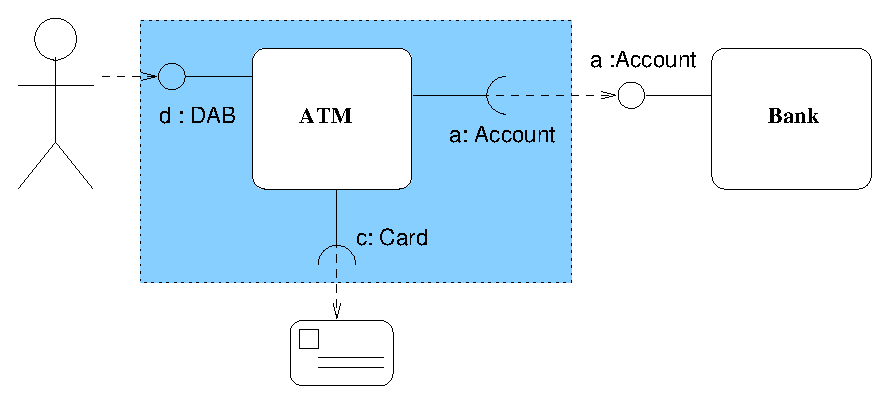
\includegraphics[width=.8\textwidth]{figures/fig-gab.eps}    
    \caption{Sch\'ema du guichet automatique}
    \label{fig-gab}
\end{figure}

Le composant ATM est le plus int\'eressant et c'est celui que nous
utiliserons par la suite dans l'illustration des techniques de
tests. Il offre une interface --- implicitement \texttt{unique} ---
permettant de r\'ealiser diverses op\'erations et requiert deux
ports : un port de type \texttt{Card} repr\'esentant le lien avec la
carte bancaire du client et un autre de type \texttt{Account}
repr\'esentant le lien avec la banque.

\begin{figure}[htbp]
\begin{lstlisting}
module Banque {
   exception error {};
   exception keep_card {};

  interface Card {...
  interface DAB { ...
  interface Account { ...

   component ATM {
      provides DAB d;
      uses Account a;
      uses Card    c;
      
   };
   
};
\end{lstlisting}
\centering
    
    \caption{Exemple de sp\'ecification \textsf{FIDL} : module Banque}
    \label{fig-exbanque}
\end{figure}

L'interface \texttt{Card} est d\'etaill\'ee dans la figure
\ref{fig-exifacecard}. Le num\'ero de compte est
stock\'e dans la carte et est donc le m\^eme pour toute la
dur\'ee d'une session, d'o\`u la d\'eclaration de
la variables $n$ englobant tous les \'echanges de messages. Le r\'esultat de
la m\'ethode \texttt{checkCode} est comme on peut s'y attendre
d\'ependant du code \og saisi\fg{} et est laiss\'e au soin de
l'implantation. Enfin la m\'ethode \texttt{failedCode} calcule le
nombre  de fois o\`u un code incorrect a \'et\'e saisi --- en examinant
toutes les r\'eponses \texttt{false} de la m\'ethode
\texttt{checkCode} --- et retourne cette valeur.

\begin{figure}[htbp]
\begin{lstlisting}
  interface Card {
    boolean checkCode(in long code); 
    long    failedCode();
    long    accountNo();

    /*** 
     header
       failed : Trace -> long
    FIDL
       n in (checkCode(_:_) +
        (f: f == failed(Trace) in failedCode(:f)) +
        accountNo(:n)))*

     body
       failed (~<-checkCode(False) : h) = (failed h) + 1;
       failed (_ : h) = failed h;
       failed [] = 0
    */
  };
\end{lstlisting}
    \centering
    
    \caption{Exemple de sp\'ecification FIDL : interface Card}
    \label{fig-exifacecard}
\end{figure}


L'interface \texttt{DAB}, figure \ref{fig-exifacedab}, d\'ecrit le comportement du guichet
automatique du point de vue du client. Le dialogue commence par
l'insertion de la carte, puis la saisie du code PIN et enfin les
diverse op\'erations. Cette interface sp\'ecifie en particulier que
les op\'erations ne sont accessibles que si le code saisi est correct
et si le nombre de saisies incorrectes est inf\'erieur \`a
3. L'exception \verb+keep_card+ peut-\^etre lev\'ee par chacune des
diff\'erentes m\'ethodes : elle signifie que la carte est
conserv\'ee par le guichet automatique et que plus aucune
op\'eration n'est possible avant de refaire une nouvelle
op\'eration \texttt{insert()} mod\'elisant le fait qu'une nouvelle
carte est introduite.

\begin{figure}[htbp]
    \centering
\begin{lstlisting}
   interface DAB {
     void    insert() raises (keep_card);
     boolean pinCode(in long code) raises (keep_card);
     void    withdrawCard () raises (keep_card);
     boolean withdrawal (in long amount) raises (keep_card);
     boolean transfer (in long amount,in long toAccountNo) raises (keep_card,error);
     long    balance () raises (keep_card);
     
     /*** FIDL
        (insert()
        ( 
          ((pinCode(_:false) + void) ( pinCode(_:false) + void)  pinCode(_:true)
            (
              withdrawal(_:_) +
              balance(:_) +
              -> transfer(_,_) (<-transfer(_) +  <-transfer<error>)) 
            )* withdrawCard() 
            ) 
            +
        ( 
           pinCode(_:false) pinCode(_:false) pinCode(_:false) 
           (
            (->withdrawal(_) <-withdrawal<keep_card>) +
            (->balance() <-balance<keep_card>) +
            (->transfer(_,_) <-transfer<keep_card>) +
            (->withdrawCard() <-withdrawCard<keep_card>)
           )
        ))*
       
     */
   };
\end{lstlisting}

    \caption{Exemple de sp\'ecification \textsf{FIDL} : interface DAB}
    \label{fig-exifacedab}
\end{figure}
 
Cet exemple relativement simple permet toutefois d'illustrer les
principaux concepts des sp\'ecifications \textsf{FIDL} dans le cas de
composants sans sp\'ecification propre. 

\subsection{Un syst\`eme de vote \'electronique}

Le deuxi\`eme exemple est celui d'un syst\`eme de vote
\'electronique. L'architecture du syst\`eme de vote est
repr\'esent\'ee sch\'ematiquement sur la  figure
\ref{fig-archivote} : il existe un certain nombre de composants
individuels de \emph{vote \'electronique} qui sont connect\'es \`a un
\emph{centre de vote} au travers d'une interface \texttt{Vote\_Center}
leur permettant de transmettre le vote --- un choix binaire ; et qui
par ailleurs peuvent recevoir un \'ev\'enement signifiant la
cl\^oture du scrutin --- type \texttt{Closure} --- et contenant le
r\'esultat du vote.

\begin{figure}[htbp]
    \centering
    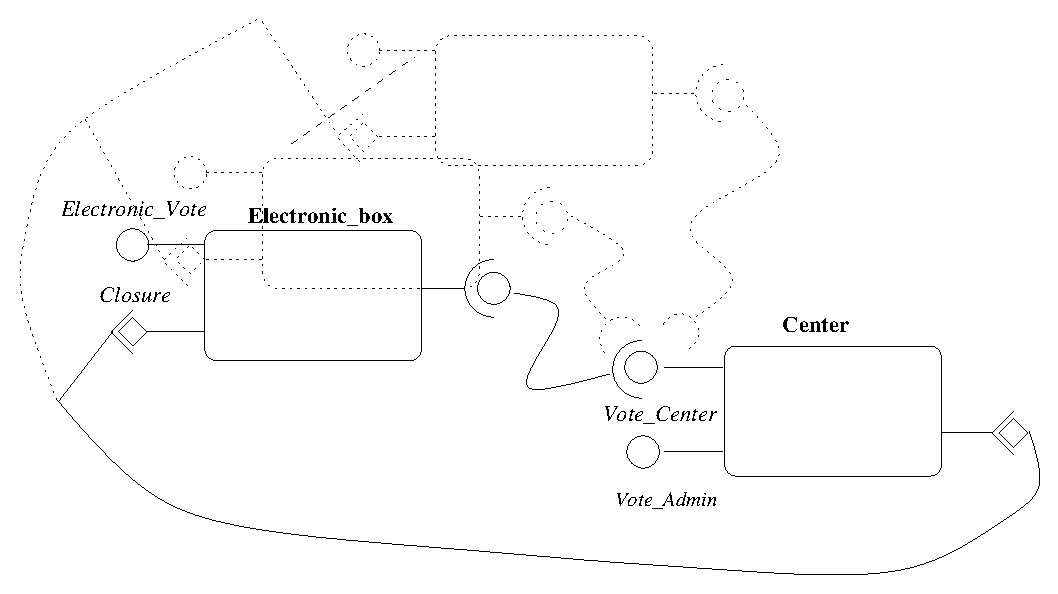
\includegraphics[width=.8\textwidth]{figures/exemple_vote.eps}
    \caption{Architecture du syst\`eme vote}
    \label{fig-archivote}
\end{figure}

Les types de donn\'ees utilis\'es sont d\'efinis dans le module
\texttt{Vote}, figure \ref{fig-exvote} : diverses exceptions, la
structure de l'\'ev\'enement de fermeture du scrutin et les
composants et interfaces. 

\begin{figure}[htbp]
    \centering
\begin{lstlisting}
module Vote { 
  exception too_late {};
  exception already_voted {};
  exception already_closed {};
  exception not_closed {};
  
  eventtype Closure {
    attribute long yes_number;
    attribute long no_number;
  };
  interface Electronic_Vote{ ...
  interface Vote_Center { ...
  interface Vote_Admin { ...
  component Center { ...
  component Electronic_Box { ...

};  
\end{lstlisting}
        \caption{Exemple 2 : module Vote}
    \label{fig-exvote}
\end{figure}

L'interface \texttt{Electronic\_Vote} (figure \ref{fig-exifacevote}) repr\'esente l'interaction
entre chaque bo\^{\i}te individuelle de vote et l'utilisateur. Son
fonctionnement est simple : elle permet \`a l'utilisateur de voter
une et une seule fois, et refuse pendant un certain temps de fournir
le r\'esultat du scrutin, puis fournit toujours le m\^eme r\'esultat. On notera l'utilisation
de l'op\'erateur  \verb+||+ qui permet d'entrelacer
arbitrairement les appels aux diff\'erentes m\'ethodes de
l'interface --- tout en respectant les r\`egles de formation correcte
des \'echanges de messages, et le fait que rien n'est dit dans l'interface quant au
moment o\`u le r\'esultat est disponible.

\begin{figure}[htbp]
    \centering
\begin{lstlisting}
  interface Electronic_Vote{ 
    boolean vote (in boolean choice);
    boolean results(out long yes,out long no);
    
    /*** FIDL
       (c in vote(c:true) + void) (c in vote(c : false) )*
     ||(results(_,_:false)*(x,y in results(x,y:true)*)) 
    */
  };
\end{lstlisting}
        \caption{Exemple 2 : interface de vote \'electronique}
    \label{fig-exifacevote}
\end{figure}
  
L'interface suivante, \texttt{Vote\_Center}, est fournie par le centre
de vote pour r\'ecup\'erer les diff\'erents votes. Son
fonctionnement est sym\'etrique de celui de l'interface
pr\'ec\'edente : elle permet de voter une et une seule fois, et
\'eventuellement elle interdit le vote si celui-ci survient trop
tard. L'interface d'administration, enfin, permet de clore le
scrutin une et une seule fois (voir figure \ref{fig-exifacecenter}).

\begin{figure}[htbp]
    \centering
\begin{lstlisting}
  interface Vote_Center {
    void vote (in boolean choice) raises (too_late,already_voted);
    
        /*** FIDL
           (x  in vote(x)) (x  in ->vote(x) <-vote<already_voted> + void)*
           (x in ->vote(x) <-vote<too_late> )* 
        */
  };
    
  interface Vote_Admin {
    void close() raises (already_closed);
    
      /*** FIDL
        close() (->close() <-close<already_closed>)*
      */
  };
\end{lstlisting}
        \caption{Exemple 2 : interfaces centre de vote \& administration}
    \label{fig-exifacecenter}
\end{figure}


Les sp\'ecifications des composants sont ici bien plus
int\'eressantes car elles permettent de \emph{mettre en musique} le
comportement des interfaces et de pr\'eciser, par exemple,
l'ordonnancemnt des diff\'erents \'ev\'enements. Le composant \texttt{Center}
est d\'etaill\'e dans la figure \ref{fig-excenter} : c'est lui qui
calcule le r\'esultat du vote en fonction des votes re\c{c}us et
effectivement pris en compte (fonction \texttt{result}) et qui
pr\'ecise \`a l'aide de l'op\'erateur de composition \texttt{and} comment
la cl\^oture du vote interagit avec les votes. Le choix fait dans
cette sp\'ecification est que tout vote survenant apr\'es un
\emph{appel} de \texttt{close()} n'est plus pris en compte, un autre
choix possible e\^ut \'et\'e de  prendre quand m\'eme en compte
ces votes. 
 
\begin{figure}[htbp]
    \centering
\begin{lstlisting}
  component Center { 
    
    provides Vote_Center v;
    provides Vote_Admin a;
    publishes Closure c;
    /***
        header
        result : Trace, boolean -> long

        FIDL
           a->close() (x : x == result(Trace,true), 
                       y : y == result(Trace,false) in c[x,y])
           a<-close() a.close<already_closed>*
         and 
           (v.vote(_) (x in v->vote(x) v<-vote<already_voted>)* + void)
           (
               (a.close() (a.close<already_closed>* || 
                           (v->vote(_)v<-vote<too_late>)*)) 
               +            
               (a->close() || v->vote(_)) 
               (v<-vote<too_late> (v->vote(_)v<-vote<too_late>)* ||
                a<-close() (a->close() a<-close<already_closed>)*)
           )
            
           body
           result [] _  =  0;
           result (~v->vote(x) : ~v<-vote() : h) y = if x == y 
                                                     then (result h x) + 1 
                                                     else (result h x);
        */
  };
\end{lstlisting}
        \caption{Exemple 2 : composant centre de vote}
    \label{fig-excenter}
\end{figure}

Le composant \texttt{Electronic\_Box} enfin (figure
\ref{fig-exevote}), permet de pr\'eciser le comportement de
l'interface de vote \'electronique en relation avec l'\'ev\'enement
de notification de fermeture du scrutin. 

\begin{figure}[htbp]
    \centering
\begin{lstlisting}
  component Electronic_Box {
    provides Electronic_Vote e;
    uses Vote_Center v;
    consumes Closure c;
        
        /*** FIDL
               (x  in e->vote(x) ( v.vote(x) e<-vote(:true) + 
                                   v->vote(x) v<-vote<too_late> e<-vote(:false)
                                 )
               ) e.vote(_:false)*
           and 
               e.results(_,_:false)
               (x,y in (c[x,y] + e->results() c[x,y] c[_,_]*
               e<-results(x,y:true)) (e.results(x,y:true)* || c[_,_]*))
        */
  };
\end{lstlisting}
        \caption{Exemple 2 : composant bo\^{\i}te individuelle de
           vote }
    \label{fig-exevote}
\end{figure}

On voit donc bien que c'est la sp\'ecification des composants qui
donne la s\'emantique du syst\`eme de vote et qui a pour fonction
d'assurer simultan\'ement l'unicit\'e des votes r\'ealis\'es au
moyen de chacune des bo\^{\i}tes \'electroniques, ce qui est
sp\'ecifi\'e par l'interface de vote \'electronique ; et par
ailleurs de garantir que tous les votes effectu\'es avant la
cl\^oture du scrutin soient pris en compte dans le d\'ecompte final
des voix qui d\'epend justement de la cl\^oture du scrutin. 
On verra  au chapitre consacr\'e \`a la composition
comment \`a partir de ces sp\'ecifications on peut esp\'erer
v\'erifier certaines propri\'et\'es du syst\`eme.



% $Log : fidl.tex,v $
% Revision 1.25  2004/10/18 09:16:33  bailly
% suppression etat art g\'en\'eral
% ajout etat art par partie (composants et test)
%
% Revision 1.24  2004/06/08 15:38:53  bailly
% *** empty log message ***
%
% Revision 1.23  2004/06/02 15:32:44  bailly
% merging
%
% Revision 1.22  2004/06/02 07:23:07  bailly
% promotion en chapitre des sections modeles et automates
%
% Revision 1.21  2004/03/29 09:26:14  bailly
% Corrections ISA suite
%
% Revision 1.20  2004/03/26 16:37:36  bailly
% *** empty log message ***
%
% Revision 1.17  2004/03/01 15:01:39  bailly
% Corrections FIDL
%
% Revision 1.16  2004/02/25 12:39:16  bailly
% Fin correction ISa sur langage FIDL
% Modification calcul ens traces de composite, syst\`eme, agencement
% Modification calcul environnement
%
% Revision 1.15  2004/02/24 08:35:55  bailly
% *** empty log message ***
%
% Revision 1.14  2004/02/24 08:26:37  bailly
% *** empty log message ***
%

%%% Local Variables: 
%%% mode: latex
%%% TeX-master: "these"
%%% End: 

\chapter{Automates \textsf{FIDL}}
\label{cha:automates-fidl}
% revoir def automates : P(Lambda), P(K)
% revoir preuve des automates bien-form\'es
% ajouter variables apparaissant seules dans les messages pour
% construction automate
%
 
Ce chapitre est une pr\'esentation formelle de l'outil principal
permettant de mod\'eliser les comportements de composants et
d'interfaces dans les mod\`eles \textsf{FIDL}. Ces comportements sont
donc mod\'elis\'es par une certaine classe d'automates, appel\'es
automates \textsf{FIDL}, dont la principal caract\'eristique est de
reconna\^{\i}tre un langage sur un certain alphabet de messages,
potentiellement inifini, \`a partir d'un
alphabet plus restreint comprenant des variables et des contraintes sur
ces variables. 

La premi\`ere partie de ce chapitre d\'efinit les automates
\textsf{FIDL} et surtout leur comportement, c'est \`a dire le langage
qu'ils reconnaissent et dont la d\'efinition n\'ecessite
l'utilisation d'un \emph{environnement}. La seconde partie d\'efinit
des expressions, similaires aux expressions rationnelles, gr\^ace
auxquelles on peut textuellement d\'ecrire un automate
\textsf{FIDL}. La troisi\`eme section, enfin, est consacr\'ee aux
probl\`emes de la v\'erification des entit\'es d\'efinies au
moyens d'automates FIDL et plus particuli\`erement au probl\`eme
du traitement  des types de donn\'ees et de la r\'esolution des
contraintes. 

\section{Les automates \textsf{FIDL}}
\label{sec:les-automates-fidl}

Apr\`es quelques pr\'eliminaires destin\'es \`a fixer les
notations et conventions math\'ematiques utilis\'ees dans ce
chapitre, nous d\'efinissons donc formellement un automate
\textsf{FIDL} et le langage qu'il reconna\^{\i}t. La d\'efinition  de
ce langage prend en compte par ailleurs les probl\`emes de
non-d\'eterminisme de l'automate et s'int\'eresse au cas d'automates
synchronis\'es. Les contraintes associ\'ees \`a la d\'efinition du
processus de reconnaissance dans un tel automate nous am\`ement in
fine \`a pr\'eciser des propri\'et\'es de \emph{bonne formation}
des automates.

\subsection{Pr\'eliminaires}
\label{sec:notations}

\subsubsection{Mono\"{\i}des, morphismes}

Pour tout ensemble $X$, $X^*$ d\'enote le mono\"{\i}de libre engendr\'e par
$X$. Par convention, $X$ sera appel\'e alphabet et sera
consid\'er\'e comme \emph{\`a priori} fini et non vide, sauf
indication explicite du contraire. Un morphisme de mono\"{\i}de
$\alpha:X^* \rightarrow Y^*$ est une 
application qui \emph{pr\'eserve} la structure de mono\"{\i}de : 
\begin{eqnarray}
\forall u,v \in X^*, \alpha(uv)=\alpha(u)\alpha(v),\label{eq:monoide} \\
\alpha(\epsilon)=\epsilon ,
\end{eqnarray} 
o\`u l'op\'eration de composition interne de chacun des mono\"{\i}des
est simplement d\'enot\'ee par la concat\'enation des mots. Un morphisme
est alphab\'etique si $\alpha(X)\subseteq Y\cup \{\epsilon\}$. Une
\emph{projection} $\Pi_{\mathrm Y}:X^* \rightarrow Y^*$ est un morphisme
alphab\'etique tel que $Y\subseteq X$ et 
$$\forall x \in X, \Pi_{{\mathrm Y}}(x) =
\left\{\begin{array}{l}x \mbox{~si~} x \in Y,\\ 
\epsilon \mbox{~si~} x \not\in Y.
\end{array}\right.$$

Pour tout $X$, on note $\#$ le morphisme de $(X^*,\epsilon,.)$ dans $(\mathbb{N},0,+)$ tel que :
$$
\begin{array}{lrcl}
\#:&X^*&\rightarrow \mathbb{N} \\
&\epsilon&\mapsto&0\\
&x&\mapsto&1\quad (x\in X) \\
&u.v&\mapsto& \#u+\#v, \\
\end{array}
$$
autrement dit $\#$ est la fonction donnant la \emph{longueur} d'un mot. 

Soit $h_a^b : X\rightarrow Y$ le morphisme d\'efini pour tout $a\in
X, b\in Y$, par 
$$
h_a^b(x) =\left\{\begin{array}{l}b \mbox{~si~} x=a,\\ 
x \mbox{~sinon~}.
\end{array}\right.
$$
Soit $X_1\times{}\dots \times{}X_n$, le produit cart\'esien de $n$
alphabets, $n\geq 2$, on a 
$$
h_{a}^b((x_1,\dots,x_n)) = (h_a^b(x_1),\dots,h_a^b(x_1)),
$$
et on notera $h_{a_1,a_2,\dots,a_n}^{b_1,b_2,\dots,b_n}$ le morphisme
d\'efini par 
$$
h_{a_1,a_2,\dots,a_n}^{b_1,b_2,\dots,b_n}(x) = \left\{\begin{array}{ll}
        b_i, &\mbox{~si~} \exists 1\leq i\leq n, x = a_i,\\
        x, &sinon 
\end{array}\right..
$$

L'alphabet d'un
langage $L$ est not\'e $\ialph(L)$. S'il n'est pas d\'efini
pr\'ecis\'ement, c'est l'ensemble des 
lettres qui composent les mots de ce langage. On parlera aussi
d'alphabet \emph{induit} par le langage $L$.

\subsubsection{Produits de m\'elange \& synchronisation}

Le produit de \emph{m\'elange}  --- \emph{shuffle} --- des mots $u\in
X^*$ et
$v\in Y^*$, not\'e $u \sh v$ est d\'efini par :
\begin{equation}
u \sh v = \{u_1v_1\dots u_nv_n \mid u =
u_1\dots u_n, v = v_1\dots v_n, \forall 1\leq i \leq n, u_i\in X^*,v_i \in Y^*\}.\label{eq:def-sh}
\end{equation}
Le produit de m\'elange de deux langages $L_1$ et $L_2$ est :
$$L_1 \sh L_2 = \bigcup_{u \in L_1, v\in L_2} u \sh v.$$

Le \emph{produit de synchronisation}\cite{dub86phd} --- ou  \emph{mixage}
--- de deux langages $L_1$ et $L_2$
sur les alphabets $X_1$ et $X_2$, not\'e $L_1 \mix_{X_1,X_2} L_2$  est d\'efini par :
\begin{equation}
L_1 \mix_{X_1,X_2} L_2 = \{u \in (X_1 \cup X_2)^* \mid
\Pi_{X_1}(u) \in L_1 \mbox{~et~} \Pi_{X_2}(u) \in L_2
\}.\label{eq:def-mix}
\end{equation}
Cette op\'eration est associative :
$$\begin{array}{lcl}(L_1) \mix_{X_1,X_2} (L_2) \mix_{X_2,X_3} (L_3) &=& ((L_1) \mix_{X_1,X_2} (L_2)) \mix_{X_1 \cup X_2,X_3} (L_3)\\
&=&  (L_1)_{X_1,X_2 \cup X_3} \mix ((L_2) \mix_{X_2,X_3} (L_3))\\
\end{array}$$ 
Lorsque plusieurs langages sont mix\'es ou m\'elang\'es, on
utilisera les 
symboles $\bigmix$ et $\bigsh$. De plus, si les alphabets utilis\'es
sont les alphabets induits, on \'ecrira plus simplement $L_1\mix
L_2$. Clairement, si $X_1 \cap X_2 =\emptyset$, alors $L_1\mix L_2 =
L_1 \sh L_2$. 

Pour tout langage $L\in X^*$, $Pref(L)$ est la cl\^oture de $L$ par ses
facteurs gauches :
$$
Pref(L) = \{v\in X^* \mid \exists u\in L, w\in X^*, u=vw\}.
$$


Pour un ensemble quelconque $X$, ${\cal P} X$ est l'ensemble des parties de
$X$.

\paragraph{Donn\'ees \& Types}

${\cal D}$ d\'esigne l'\emph{univers} des valeurs primitives, ses
\'el\'ements sont appel\'es aussi litt\'eraux, par opposition aux
variables. Un \emph{type}  $T$ est un sous-ensemble de
${\cal D}$ et nous noterons ${\cal D}_T$ le domaine des valeurs de ce
type. $Type(v)$ d\'esignera le type d'une variable ou d'un
identifiant $v$. ${\cal V}$ est un ensemble d\'enombrable de noms de
variables disjoint de ${\cal D}$.

Sym\'etriquement, on peut d\'efinir $\cal D$ comme l'ensemble r\'esultant de l'union de tous les domaines de
tous les types $T$. Nous ne donnons pas ici de description formelle
d'un syst\`eme de type permettant de construire explicitement un type
$T$ et l'ensemble des valeurs $\cal D$ consid\'erant que cette
formalisation n'est pas n\'ecessaire pour le reste de la
d\'efinition du langage \textsf{FIDL}. 

Dans l'imm\'ediat, nous consid\'ererons que l'on dispose d'un
ensemble de types primitifs tels que les entiers, les bool\'eens, les
cha\^{\i}nes de caract\`eres et de types inductifs --- sans variables
de types --- construits \`a partir de constructeurs de types tels que les
structures et les s\'equences.

\subsubsection{Graphes}

Un multigraphe dirig\'e $G=(S,E)$ est un couple o\`u $S$ est un ensemble fini de sommets et
$E$ un ensemble fini d'arcs d\'efini au moyen d'un couple
d'applications $\iota:E\mapsto S,\omega:E\mapsto S$ associant \`a
chaque \'el\'ement de $E$ un sommet de d\'ebut et un sommet  de
fin. Dans le cas de graphes dirig\'es simples, si $\iota \times{}
\omega$ est une fonction injective, on d\'ecrira les
\'el\'ements de $E$ simplement par le couple $(s,t)$
d'\'el\'ements de $S$ de d\'ebut et de fin de l'arc. 

Une \emph{cha\^{\i}ne} est une s\'equence ordonn\'ee $\mu{}= s_1e_1s_2e_2 \dots s_{k_1}e_{k-1}s_k$
d'\'el\'ements de $S$ et $E$ telle que  pour tout arc $e_i, 1<i<n$,
$\iota(e_i) = s_i, \omega(e_i) = s_{i+1}$.

Un $(s,t)$-\emph{chemin} est une cha\^{\i}ne telle que pour tout
\begin{itemize}
  \item chaque arc n'appara\^{\i}t qu'une seule fois : $\forall e_i,e_j,
    i\neq j \implies e_i\neq e_j$ ;
  \item chaque sommet n'appara\^{\i}t qu'une seule fois : $\forall
  s_i,s_j, i\neq j \implies s_i\neq s_j$ ;
  \item $s_1 = s$,  $s_k=t$.
\end{itemize}

Pour toute cha\^{\i}ne et tout chemin $\mu{}$, $E(\mu{})[i]$ d\'esigne
l'arc $e_i$ de la cha\^{\i}ne $\mu{}$ et $S(\mu{})[i]$ le sommet $s_i$ de
$\mu{}$. La taille d'une cha\^{\i}ne, not\'ee $\vert \mu{}\vert$ est le
nombre de sommets parcourus par la cha\^{\i}ne. 

Un \emph{cycle} est une cha\^{\i}ne telle que $s_1 = s_k$. Un cycle est
\emph{\'el\'ementaire} si chaque $e_i$ appara\^{\i}t une et une seule
fois dans la cha\^{\i}ne.  

Un automate $A=(Q,I,T,\Sigma,\delta)$ peut \^etre vu comme  un
multigraphe $G=(Q,\delta)$ tel que pour tout $d=(q,a,q') \in \delta$,
$\iota(d) =q$ et $\omega(d) = q'$, muni de deux fonctions :
\begin{itemize}
  \item une fonction $I:Q\rightarrow \mathbb{B}$ identifiant les
  \'etats initiaux ;
\item une fonction $T:Q\rightarrow \mathbb{B}$ identifiant les
  \'etats terminaux. 
\end{itemize}

\subsection{Automates}

\begin{definition}[Automate \textsf{FIDL}]
Un automate \textsf{FIDL} est un quintuplet
$$A = (Q,q_0,T,\Sigma \times{}{\cal P}\Lambda \times{}{\cal P}\mathcal{K},\delta)\ ,$$
o\`u $Q$
est un ensemble d'\'etats, $q_0$, l'\'etat initial, un \'etat distingu\'e de
$Q$, $T$ un sous-ensemble de $Q$ contenant les \emph{\'etats finaux}, $\Sigma$
un alphabet, $\Lambda$ un ensemble \emph{fini}
de variables, $\mathcal{K}$ un ensemble
fini de contraintes sur $\Lambda$ et
$\delta$ une relation de transition entre $Q \times{}(\Sigma \times{}\Lambda \times{}\mathcal{K})$ et $Q\setminus q_0$.
\end{definition}

Ce qui distingue fondamentalement un automate \textsf{FIDL} d'un
automate classique c'est qu'il reconna\^{\i}t un langage qui n'est pas
constitu\'e uniquement des lettres de son alphabet. L'automate est
construit sur un alphabet contenant
des variables, variables qui sont contraintes par des fonctions et
pr\'edicats. L'ensemble des substitutions ou interpr\'etations de
variables respectant les contraintes d\'efinit le langage en terme de
lettres \og closes\fg.

\subsection{Alphabet}
\label{sec:alphabet}
Les lettres de l'alphabet $\Sigma$ d'un automate \textsf{FIDL}  sont
des couples constitu\'es d'une \emph{enveloppe}, identifi\'ee
g\'en\'eralement par $m$ et appartenant \`a un ensemble ${\cal X}$, et 
d'un \emph{contenu}, \'eventuellement vide, qui est un n-uplet
constitu\'e de valeurs litt\'erales ou de variables. Ces lettres sont appel\'ees
\emph{messages} et sont not\'ees $m(x_1,\dots,x_{ar(m)})$.

Toute enveloppe poss\`ede une arit\'e et une
signature qui pr\'ecisent le nombre des \'el\'ements du n-uplet
contenu dans le message ainsi que leur type, c'est \`a dire
l'ensemble des valeurs admissibles. Plus formellement, pour tout  $m\in
{\cal X}$, $ar(m)
\in \N$ est l'\emph{arit\'e} de $m$ et pour chaque indice $i\in
\{1,\dots,ar(m)\}$, $m[i]$ est le type 
$T$ du $i^{eme}$ param\`etre. Si $ar(m)=0$, $m$ est un message constant sans contenu. 

L'ensemble de tous les messages, pour un ensemble d'enveloppes $\cal X$, est not\'e ${\cal E}$ et se
d\'efinit comme :
$$
{\cal E } = \{ m(x_1,\dots,x_n) \mid m\in {\cal X},n =ar(m), x_i \in {\cal V}\cup m[i]\}.
$$
L'alphabet d'un automate $\Sigma$ est donc une partie \emph{finie}  de
$\cal E$. L'ensemble des \emph{messages clos} est la  partie de $\cal E$
qui contient uniquement les messages avec un contenu sans
variables. Cet ensemble est not\'e $\bar{\cal E}$ et d\'efini comme :
$$
\bar{\cal E } = \{ m(v_1,\dots,v_n) \mid m\in {\cal X},n =ar(m), v_i \in  m[i]\}.
$$

On d\'efinit $var(\Sigma)$, l'ensemble des variables
apparaissant dans les messages de  $\Sigma$ :
$$
var(\Sigma) = \bigcup_{m(x_1,\dots,x_{ar(m)}) \in \Sigma}\{x_i\in {\cal V}, \mbox{~pour~}
1\leq i\leq ar(m) \}.
$$

\subsection{Variables \& Contraintes}

\`A chaque automate \textsf{FIDL} correspond un ensemble de
contraintes $\cal K$ et un ensemble de variables $\Lambda$. Chaque
contrainte $c\in {\cal K}$ est constitu\'ee d'un pr\'edicat $P:{\cal D}^r\rightarrow
\mathbb{B}$ d'arit\'e $r$ et de deux ensembles de
variables, les variables li\'ees $bv(c)\subseteq \Lambda$ et les
variables libres $fv(c)\subseteq
\Lambda$, tels que pour une contrainte $c$ :
\begin{itemize}
  \item $bv(c) \cap fv(c) =\emptyset$ ;
  \item $var(c) = bv(c)  \cup fv(c)$ ;
  \item $\vert bv(c) \vert = 1$.
\end{itemize}

Par extension, on d\'efinit pour un automate $A$ l'ensemble des
variables li\'ees et libres de $A$ :
\begin{align*}
    bv(A) = \bigcup_{c\in {\cal K}} bv(c) &\qquad\mbox{~et~}\qquad&
    \begin{array}{rcl}
fv(A) &= &(var(\Sigma) \cup \bigcup_{c\in {\cal K}} fv(c) )
    \setminus bv(A) \\
&=& \Lambda \setminus bv(A).
\end{array}
\end{align*}

L'identifiant $\mathtt{Trace}$ d\'esigne une variable sp\'eciale,
pr\'esente dans tous les automates \textsf{FIDL}, et qui a pour
fonction de permettre la d\'efinition de contraintes et de fonctions
d\'ependant de l'historique de l'ex\'ecution de l'automate dans
lequel elles sont utilis\'ees. Cette variable ne peut appara\^{\i}tre
dans le contenu d'un message. 

\subsection{Langage reconnu par un automate \textsf{FIDL}}
\label{section-reco}

Le langage reconnu par un automate \textsf{FIDL} est
constitu\'e de mots  construits
sur l'ensemble des message clos $\bar{\cal E}$ : formellement, le
langage d'un automate $A$ est donc inclus dans $\bar{\cal E}^*$. 
 Dans un \'etat donn\'e de l'automate, il faut donc faire
correspondre \`a une lettre de l'alphabet formel $\Sigma$ sur lequel est
construit l'automate
une ou plusieurs lettres de l'alphabet r\'eel de l'ensemble des
mots reconnus par l'automate. Par exemple, \`a un message
not\'e $m(v_1,\dots,v_n)$,
o\`u $v_1,\dots,v_n$ est le contenu 
effectif du message, doit correspondre une transition
$(m(x_1,\dots,x_n),V,C)$ qui peut \^etre d\'eclench\'ee  dans
l'\'etat courant.

Dans l'\'etiquette d'une transition, certains des $x_i$ peuvent \^etre
interpr\'et\'es comme des valeurs litt\'erales, auquel cas $v_i$ doit \^etre la m\^eme valeur.
D'autres $x_j$ peuvent \^etre des variables, soit introduites dans $V$ et
contraintes par $C$, soit comme partie de l'\'etiquette d'une
transition menant \`a l'\'etat courant. Dans ce second cas, $v_j$ doit satisfaire la
contrainte associ\'ee \`a $x_j$ ou la valeur pr\'ec\'edemment \og choisie\fg
pour $x_j$. D'autres $x_i$ encore peuvent \^etre des variables
libres, c'est \`a dire ne correspondre \`a aucune contrainte.
Par cons\'equent, nous devons m\'emoriser lors du parcours de l'automate
le lien entre un nom de variable et sa valeur dans un
\emph{environnement}.

\begin{definition}[Environnement]
L'environnement d'un calcul not\'e $\sigma$ --- pour \emph{store}  --- est
un triplet $(V,val,pred)$ o\`u :
\begin{itemize}
  \item $V\subset \cal V$ est un ensemble fini de variables ;
\item $val : V\rightarrow {\cal D}\cup \{\bot\}$ est une fonction
  totale de \emph{valeur} ou \emph{valuation} assignant \`a chaque variable
  une valeur dans $\cal D$, les valeurs ind\'efinies
  \'etant d\'enot\'ees par $\bot$, o\`u $\bot \not\in {\cal
  D}$.  ;
\item $pred: V\rightarrow({\cal D}\rightarrow
  \mathbb{B})$ est une fonction totale de \emph{contrainte}
  assignant \`a chaque variable un pr\'edicat sur ${\cal D}$ qui est
  une fonction de l'ensemble des valeurs dans l'ensemble des
  bool\'eens $\{\mathtt{true},\mathtt{false}\}$. Par abus de langage
  nous d\'esignerons par $\mathtt{true}$ --- resp. $\mathtt{false}$
  --- la fonction constante  $\lambda x.\mathtt{true}$ --- resp.  $\lambda x.\mathtt{false}$.
\end{itemize}
Pour un environnement $\sigma$ on note $V_\sigma$, $val_\sigma$ et
$pred_\sigma$ les diff\'erents composants de l'environnement,
l'indice \'etant omis lorsque l'environnement est clairement
pr\'ecis\'e par le contexte.
\end{definition}

Nous d\'efinissons maintenant un pas de l'ex\'ecution d'un automate
\textsf{FIDL} $A=(Q,q_0,T,\Sigma \times{}{\cal P}\Lambda
\times{}{\cal P}\mathcal{K},\delta)$, \`a partir d'un couple $(q,\sigma)$
form\'e de l'\'etat courant de
l'automate $q\in Q$ et d'un environnement associ\'e.

\paragraph{D\'eclenchement d'une transition}
Soit un automate $A$ dans un \'etat $q$ associ\'e \`a un
environnement $\sigma=(V,val,pred)$, et une lettre $a = m(v_1,\dots,v_n)$, l'automate peut atteindre l'\'etat $q'$ s'il existe
une transition $(q,(m(x_1,\dots,x_n),
W,K),q')$ dans $A$ telle que pour tout $i$, $1\leq i\leq n$ :
\begin{itemize}
  \item soit $x_i$ est un litt\'eral et $v_i=x_i$. La transition est
  d\'efinie avec une valeur litt\'erale qui doit \^etre
  identique \`a la valeur contenue dans le message ;
\item soit $x_i$ est une variable d\'efinie dans $W$ et
  $K(v_i)=\mathtt{true}$. La variable $x_i$ est d\'eclar\'ee et
  contrainte localement et la contrainte est respect\'ee par $v_i$ ;
\item soit $x_i\not\in W$ est une variable et  $x_i \in
  V$, c'est \`a dire que la variable sur la transition a \'et\'e
  d\'eclar\'ee et contrainte pr\'ec\'edemment, alors :
  \begin{itemize}
    \item soit $val_\sigma(x_i)=v_i$,
    \item soit $val_\sigma(x_i)= \bot$ et $pred_\sigma(x_i)(v_i) = \mathtt{true}$.
  \end{itemize}
% \item soit $x_i$ est une variable libre et $v_i$ est une  valeur appartenant au type de $x_i$.
\end{itemize}
Cette propri\'et\'e est not\'ee
$$
(q,\sigma) \xrightarrow{a} (q',\sigma')
$$
o\`u $\sigma'=(V_{\sigma'}, val_{\sigma'},pred_{\sigma'})$ est un
nouvel environnement d\'efini  par :
$$
\begin{array}{rcl}
V_{\sigma'} &=&  V_\sigma \cup W, \\
val_{\sigma'} &=& \{x_i \mapsto v_i \mid  i \in \{1,\dots,n\} \} \\
& \cup& \{y \mapsto \bot \mid y \in W, \exists c(y) \in K,\\
&&\ \ y \neq x_i, \forall i \in \{1,\dots,n\} \} \\
& \cup & \{\mathtt{Trace} \mapsto val_\sigma(\mathtt{Trace}).a\} \\
&\cup& \{y \mapsto z \mid y \not\in W, y \in V_\sigma\setminus\{\mathtt{Trace}\}, z = val_\sigma(y)\}, \\
pred_{\sigma'}&=&  \{x_i \mapsto \mathtt{true} \mid i \in
\{1,\dots,n\} \} \\
& \cup& \{y \mapsto c \mid y \in W, \exists c(y) \in K,\\
&&\ \ y \neq x_i, \forall i \in \{1,\dots,n\} \} \\
& \cup& \{y \mapsto c \mid y \not\in W, y \in V_\sigma\setminus\{\mathtt{Trace}\}, c = pred_\sigma(y)\}\\
& \cup& \{\mathtt{Trace} \mapsto \mathtt{true}\}.\\
\end{array}
$$

La condition de franchissement d'une transition inclut outre une
condition sur l'\'egalit\'e des attributs de l'\'ev\'enement, une
v\'erification de la validit\'e des valeurs des param\`etres de
messages eu \'egard \`a l'environnement courant, c'est \`a dire aux
contraintes d\'efinies sur les variables. Ce franchissement n'est
possible que si, pour chaque param\`etre, sa valeur est \'egale \`a
celle stock\'ee pour la variable correspondante dans l'environnement
courant ou compatible avec les contraintes actuellement d\'efinies
pour cette variable.

La mise \`a jour de l'environnement --- d\'efinie ici par
cr\'eation d'un nouvel environnement $\sigma'$ --- comprend les
\'etapes suivantes :
\begin{itemize}
  \item on \'etend tout d'abord l'ancien ensemble de variables avec
  l'ensemble des variables d\'eclar\'ees dans la transition ;
\item la valuation des variables est ensuite modifi\'ee : toutes les
  occurences de variables apparaissant dans le corps du message sur la
  transition re\c{c}oivent la valeur correspondante dans le corps du
  message de l'\'ev\'enement lu, les autres variables
  d\'eclar\'ees dans la transition re\c{c}oivent la valeur
  sp\'eciale ind\'efinie $\bot$ et la trace $\mathtt{Trace}$ est
  mise \`a jour, le reste de l'environnement demeurant inchang\'e ;
\item finalement, la fonction de contrainte est mise \`a jour : le
  pr\'edicat associ\'e aux variables devenues d\'efinies devient
  $\mathtt{true}$ pour signifier qu'il n'est plus n\'ecessaire de le
  v\'erifier, les nouvelles contraintes d\'eclar\'ees sur la
  transition sont ajout\'ees \`a l'environnement et les autres contraintes restent inchang\'ees.
\end{itemize}

\paragraph{Reconnaissance}
Enfin, nous pouvons d\'efinir la reconnaissance d'un mot et par
cons\'equent l'ensemble des mots reconnus par un automate \textsf{FIDL}.
\begin{definition}
Soient $A= (Q,q_0,T,\Sigma \times{}{\cal P}\Lambda \times{}{\cal P}\mathcal{K},\delta)$ un
automate et $T=e_1 e_2 \dots e_n$ un mot avec $\forall i, 1\leq i \leq
n, e_i\in \bar{\cal E}$,
$T$ est
\emph{accept\'e} par $A$ s'il existe une s\'equence de couples
$(q,\sigma_0) \dots (q_{n},\sigma_{n})$ tels que
\begin{itemize}
  \item $q = q_0$, l'\'etat initial de $A$ et $\sigma_0 =
  (\{\mathtt{Trace}\},\{ \mathtt{Trace}\mapsto
  \varepsilon\},\{\mathtt{Trace}\mapsto \mathtt{true}\})$ ;
\item quel que soit $j$, $0\leq j < n$, $(q_j,\sigma_j)
  \xrightarrow{e_{j+1}} (q_{j+1},\sigma_{j+1})$ ;
\item $q_n \in T$.
\end{itemize}
Le langage reconnu par $A$, not\'e $L({A})$, est l'ensemble des
mots reconnus par $A$.
\end{definition}

\subsection{Reconnaissance par synchronisation d'automates}
\label{sec:reconn-par-synchr}

Soient les automates \textsf{FIDL}
$A_1,\dots,A_n$, on d\'efinit la
reconnaissance d'un mot par \emph{synchronisation des automates}
$A_1,\dots,A_n$ et donc le langage des automates synchronis\'e
$A_1,\dots, A_n$. Ceci nous permet de d\'efinir un automate
synchronis\'e $\cal A$ comme le n-uplet $(A_1,\dots,A_n)$, son
langage $L_{\cal A}$ \'etant bien entendu le langage des automates
synchronis\'e $A_1,\dots,A_n$ sans qu'il soit n\'ecessaire de
construire explicitement l'automate $\cal A$. 

L'\'etat associ\'e \`a un calcul est  un n-uplet d'\'etats \'el\'ementaires
$$((q_1,\sigma_1),\dots,(q_n,\sigma_n)).$$
Un \'ev\'enement $e=m(v_1,\dots,v_p)$ est reconnu par la machine ${\cal A}$ et permet
d'atteindre l'\'etat
$$((q_1',\sigma_1'),\dots,(q_n',\sigma_n')),$$
si pour chaque $i$, $1\leq i\leq n$ :
\begin{enumerate}
  \item si $m$ appartient \`a l'alphabet de $A_i$, c'est \`a dire
  si il existe $a=m(y_1,\dots,y_p)\in \Sigma_i$,  alors
    $$(q_i,\sigma_i) \xrightarrow{a} (q_i',\sigma_i')\ ;$$
  \item sinon, $(q_i,\sigma_i) = (q_i',\sigma_i').$
\end{enumerate}
Un mot $u=m_1 m_2 \dots m_k$ est reconnu par $\cal A$ si il existe une
s\'equence de n-uplets  $Q_0 Q_1 \dots Q_m$, avec $Q_0 =
((q_1^0,\sigma_1^0),\dots,(q_n^0,\sigma_n^0)), Q_i =
((q_1^i,\sigma_1^i),\dots,(q_n^i,\sigma_n^i)), 1\leq i$, telle que pour tout
$j, 1\leq j\leq k$, pour tout $1\leq i\leq n$,  $(q_{j}^i,\sigma_j^i)
\xrightarrow{m_i} (q_{j+1}^i,\sigma_{j+1}^i)$, $q_k^i\in T_{A_i}$.


\subsection{Automate bien-form\'e}

Il appara\^{\i}t \'evident de la d\'efinition du langage telle que
donn\'ee ci-dessus que celle-ci d\'epend des d\'eclarations de
variables et de la r\'esolution des contraintes y aff\'erent. Pour
que le processus de d\'efinition des variables dans l'environnement
en fonction des messages effectivement lus puisse se d\'erouler
correctement, il est n\'ecessaire d'imposer des r\`egles de
bonnes formation pour les automates :
\begin{itemize}
  \item toutes les variables, \`a l'exception de la variable
    $\mathtt{Trace}$ doivent \^etre d\'eclar\'ees sur la transition
    o\`u elles sont utilis\'ees ou sur une transition ayant d\'ej\`a
    \'et\'e franchie par le processus de reconnaissance ;
  \item lorsque la valeur d'une variable est contrainte par un
    pr\'edicat dans lequel apparaissent d'autres variables, celles-ci
    doivent avoir \'et\'e pr\'ealablement d\'eclar\'ees et
    d\'efinies. Cette condition implique que les contraintes ne
    peuvent \^etre r\'ecursivement d\'ependantes les unes des
    autres. 
\end{itemize}

Nous d\'efinissons tout d'abord une relation entre les diff\'erentes
contraintes utilis\'ees dans un automate en fonction de leur
interd\'ependance. 

\begin{definition}[D\'ependance des contraintes]
    \'Etant donn\'e un automate \textsf{FIDL}  $A= (Q,q_0,T,\Sigma
    \times{}{\cal P}\Lambda \times{}{\cal P}\mathcal{K},\delta)$, la relation
    de d\'ependance entre deux contraintes $c,c'$, not\'ee $c\leq c'$ est une partie
    de  ${\cal K}\times{}{\cal K}$  telle que :
    \begin{itemize}
      \item $c\leq c$ ;
      \item s'il existe un chemin $q d q' \mu{} p
      d' p'$  dans l'automate $A$, avec $d=(q,(e,V,K),q') \in \delta$,
      $d'=(p,(e',V',K'),p') \in \delta$, et des contraintes $c\in K$,
      $c' \in K'$, telles que $bv(c)\subseteq fv(c')$, alors $c\leq c'$. 
    \end{itemize}
\end{definition}

Cette relation exprime formellement le fait qu'une variable li\'ee
par une contrainte $c$ et utilis\'ee par une autre contrainte $c'$, telles
qu'il existe un chemin dans l'automate menant de l'une \`a l'autre,
induit une d\'ependance de $c'$ envers $c$.

Les propri\'et\'es de bonne formation d'un automate s'expriment
alors formellement comme :

\begin{definition}[Automate \textsf{FIDL} bien form\'e]
\label{def:automate-bien-forme}  \'Etant donn\'e un automate \textsf{FIDL}  $A= (Q,q_0,T,\Sigma
    \times{}{\cal P}\Lambda
    \times{}{\cal P}\mathcal{K},\delta)$, on note $\mu{}_{q,p}$ un 
    $(q,p)$-chemin du graphe de $A$ entre les \'etats $q$ et $q'$
    form\'e par une s\'equence de transitions de $\delta$.
 $A$ est dit bien form\'e si et seulement si
    \begin{enumerate}
      \item \label{prop-wf-circ} la cl\^oture transitive de la
      relation de d\'ependance entre contraintes $\leq$ est un
      bon-ordre partiel : elle est r\'eflexive,  transitive et
      surtout \emph{anti-sym\'etrique} ;
  \item \label{prof-wf-nofree} pour tout $c\in {\cal K}$ et toute
    transition $(q,(m,V,K),q')\in \delta$ telle que $c\in K$, pour toute
    variable libre $y\in fv(c)$, alors pour tout $(q_0,q')$-chemin $\mu{}=
    \mu{}_1 (q_1,(m',V',K'),q_2) \mu{}_2 (q,(m,V,K),q')$, il
    existe $(q_1,(m',V',K'),q_2)$ avec dans $K'$ une contrainte $c'$
    liant $y$ ;
  \item \label{prof-wf-trace} si $\mathtt{Trace} \in \Lambda$ alors,
  $fv(A) =  \{\mathtt{Trace}\}$ sinon $fv(A) = \emptyset$.  
\end{enumerate}
\end{definition}

\subsection{Non-d\'eterminisme}

Un automate \textsf{FIDL} peut \^etre non-d\'eterministe : \`a
partir d'un m\^eme \'etat, il peut exister deux transitions 
\'etiquet\'ees par le m\^eme message telles que les environnements
permettant de satisfaire les contraintes apparaissant sur les deux
transitions contiennent des valeurs de variables communes. Plus
formellement, un automate \textsf{FIDL} $A=(q_0,T,\Sigma \times{}{\cal P}\Lambda
\times{}{\cal P}\mathcal{K},\delta)$ est non d\'eterministe si, pour deux
transitions $d_1=(q,((m,x_1,\dots,x_n),
W,K),q')$ et $d_2=(q,((m,y_1,\dots,y_n),
W',K'),q'')$, il existe $\sigma,\sigma_1',\sigma_2'$ des
environnements et un mot $u=ve$ tels que :
$$
(q_0,\sigma_0)\xrightarrow{u}(q,\sigma)\xrightarrow[d_1]{e} (q',\sigma_1') \qquad \mbox{et} \qquad (q_0,\sigma_0)\xrightarrow{u}(q,\sigma)\xrightarrow[d_2]{e} (q'',\sigma_1')
$$

Or nous avons d\'efini la reconnaissance des langages  en termes d'automates
d\'eterministes. L'extension au cas des automates
non-d\'eterministes est toutefois simple : la reconnaissance dans un automate non-d\'eterministe se fait comme
d'habitude en consid\'erant \`a chaque pas de l'automate l'ensemble
des \'etats accessibles et l'union des environnements associ\'es.

Si l'on note $[q]\subseteq Q$ un \'etat de l'automate non
d\'eterministe, alors $([q],\sigma)\xrightarrow{e} ([q'],\sigma')$
ssi
$$
\forall p \in [q], \exists p' \in [q'], (p,\sigma)\xrightarrow{e} (p',\sigma_p)
$$
avec $\sigma' = \cup_{p} \sigma_p$. 

\section{Expressions \textsf{FIDL}}

Les automates FIDL sont construits \`a partir d'expressions du
m\^eme nom permettant d'exprimer la structure de l'automate sous la
forme d'une expression de type rationnelle contenant des contraintes. Nous
d\'efinissons dans cette section le processus de construction des
automates \textsf{FIDL} \`a partir des expressions. Nous faisons en
sorte de contraindre la forme des expressions pour que tous les
automates \textsf{FIDL} construits \`a partir d'expressions
syntaxiquement correctes soient bien form\'es.

\subsection{Expressions}
\label{sec:expressions}

Nous avons d\'ej\`a vus les expressions  \textsf{FIDL} de mani\`ere
informelle dans le chapitre \ref{chap-fidl}. La syntaxe est
pr\'ecis\'ee dans la figure \ref{fig-syn-fidl}. Ces expressions sont semblables aux
expressions rationnelles classiques form\'ees \`a partir de l'alphabet des messages
possibles dans le contexte de l'expression. En plus des op\'erateurs
usuels des langages rationnels, union, concat\'enation et
\'etoile, on utilise des op\'erateurs binaires pour exprimer le
produit  de m\'elange $\|$ et la synchronisation
$\mathbf{and}$. Surtout, la principale diff\'erence s'exprime dans l'utilisation  de
contraintes et de variables qui ont un impact important sur la
s\'emantique de ces expressions. Pour simplifier les
d\'efinitions qui suivent, le symbole  $\circ$ d\'esigne l'un quelconque des op\'erateurs
binaires $.$, $\|$, $+$, $\mathbf{and}$. 

\subsubsection{Syntaxe}

Ceci est un rappel de la syntaxe pr\'ec\'edemment  donn\'ee.

\begin{figure}[htbp]
\begin{minipage}[t]{.45\textwidth}
    \begin{equation}
\begin{array}{ccl}
        Expr &\quad\rightarrow\quad& Expr Expr \mid Expr^* \mid \\
        && Expr + Expr \mid (Expr) \mid \\
        && Expr \parallel Expr \mid \\
&&(Ctr\ \mathbf{in}\ Expr) \mid \\
        && Msg \mid \mathtt{void}\\
        Msg &\quad\rightarrow\quad& m(Param) \mid m() \\
        Param &\quad\rightarrow\quad& Atom \mid Atom,Param \\
        Atom &\quad\rightarrow\quad& x \mid l \\
\end{array}
\end{equation}
\end{minipage}
\begin{minipage}[t]{.45\textwidth}
    \begin{equation}
\begin{array}{ccl}
Ctr &\quad\rightarrow\quad& x : Pred \\
Pred &\quad\rightarrow\quad& \mathtt{true} \mid \mathtt{false} \mid \\
&&Pred \vee Pred \mid \neg{}Pred \mid p
(x,Fun)  \\
Fun &\quad\rightarrow\quad& f(Par) \mid l \\
Par &\quad\rightarrow\quad& Par,y  \mid y \mid Fun \mid \mathtt{Trace} \\
\end{array}
\end{equation}
\end{minipage}\centering

\caption{Syntaxe des expressions \textsf{FIDL} (interfaces)}
\label{fig-syn-fidl-rappel}
\end{figure}

Les symboles $x,y$, $l$, $p$ et $f$ sont des symboles terminaux
d\'enotant respectivement  des variables de l'ensemble ${\cal
  V}\setminus \{ \mathtt{Trace} \}$, des
litt\'eraux de l'ensemble $\cal D$, des
pr\'edicats n-aires de ${\cal D}^n$ dans $\mathbb{B}$ et des
fonctions d'arit\'es $r$ de ${\cal D}^r$ dans ${\cal D}$.

\subsubsection{R\`egles s\'emantiques}

Les expressions FIDL doivent respecter par ailleurs les r\`egles
s\'emantiques suivantes. 

\paragraph{Variables}

Les expressions FIDL contiennent des variables qui repr\'esentent des
donn\'ees transport\'ees par les messages. Pour une expression $E$,
on d\'efinit des
ensembles de variables li\'ees $bv(E)$ et libres $fv(E)$. L'ensemble
des variables de $E$, $var(E)$ est simplement d\'efini comme $var(E)
= bv(E) \cup fv(E)$. Ces
ensembles de variables sont d\'efinis inductivement par les r\`egles
suivantes :

$$
\begin{array}{rcl}
bv(E^*) &=&  bv(E), \\
fv(E^*) &=&  fv(E) \\
\\
bv(E\circ F) &=&  bv(E) \cup bv(F), \\
fv(E\circ F) &=&  fv(E) \cup fv(F) \\
\\
fv(Msg) = fv(m(x_1,\dots,x_n)) &=& \{x_i \in {\cal V},
1\leq i \leq n\}, \\
bv(Msg) = bv(m(x_1,\dots,x_n)) &=& \emptyset \\
\\
bv(Ctr\ \mathbf{in}\ E) &=& bv(E) \cup
bv(Ctr), \\
fv(Ctr\ \mathbf{in}\ E) &=& fv(E)\cup fv(Ctr) \setminus
bv(Ctr) \\
\\
fv(Ctr) = fv(x:Pred) &=& var(Pred)\setminus \{x\}, \\
bv(Ctr) = bv(x:Pred) &=& \{x\} \\
\end{array}
$$

L'op\'eration d'$\alpha$-renommage des variables permet de s'assurer
que si $E=F\circ G$, alors on a  $bv(F) \cap bv(G) = \emptyset$, $bv(F) \cap var(G) =
\emptyset$, $var(F) \cap bv(G) = \emptyset$. Les variables li\'ees
ont ainsi une port\'ee unique limit\'ee \`a l'arbre d'expression
qui suit leur introduction. 

\begin{definition}[$\alpha$-renommage]
$$
\begin{array}{rrcl}
\alpha:&L_E &\longrightarrow& L_E \\
&\alpha(\mathtt{void}) &\longmapsto& \mathtt{void}\\
&\alpha(Msg) &\longmapsto& Msg \\
&\alpha(E \circ F) &\longmapsto&
\left\{\begin{array}{ll}
\alpha(E) \circ \alpha(F),& \mbox{~si~}
bv(E) \cap var(F) = var(E) \cap bv(F) = \emptyset \\
\alpha(h_x^{x'}(E) \circ  h_x^{x''}(F)),& \mbox{~pour~} x\in bv(F)\cap bv(G),
\mbox{~avec~} x',x''\not\in var(F)\cup var(E) \\
\end{array}\right. \\
&\alpha(E^*) &\longmapsto&\alpha(E)^*\\
&\alpha(x:P(x) \mathbf{~in~} E) &\longmapsto&  x:P(x) \mathbf{~in~}
\alpha(E))\\
\end{array}
$$
\end{definition}

Une expression de contrainte est non ambig\"ue si la variable
d\'efinie et sa contrainte n'utilisent pas de variables li\'ees dans
la sous-expression associ\'ee.

\begin{property}[Expression non-ambig\"ue]
Une expression $(x:Pred\ \mathbf{in}\ Expr)$ est non-ambig\"ue si et
seulement si  
$$(x \cup
var(Pred)) \cap bv(Expr) = \emptyset.$$
\end{property}

Enfin, nous exigerons que toute expression $E$ ne contienne
comme seule variable libre que la variable $\mathtt{Trace}$ :

\begin{property}[Cl\^oture]
   Une expression $E$ est \emph{close} si et seulement si 
$$
fv(E) \subseteq \{\mathtt{Trace}\}.
$$
\end{property}

\begin{definition}[Expression bien-form\'ee]
    \label{def:exprwf}
    Une expression \textsf{FIDL} $E$ est bien form\'ee si :
    \begin{enumerate}
      \item $E$ est transform\'ee par la fonction de renommage
        $\alpha$ ;
      \item $E$ et toute ses sous-expressions sont non ambig\"ues ;
      \item $E$ est close.
    \end{enumerate}
 \end{definition}

\subsection{Construction}
\label{section-construction}
\`A partir d'une expression $E$ ne comprenant pas
d'op\'erateur de synchronisation \textbf{and} (voir chapitre
\ref{chap-fidl}, section \ref{sec:grammaire}), on construit par
induction l'automate \textsf{FIDL}
associ\'e  $A = (Q,q_0,T,\Sigma\times{}{\cal P}\Lambda\times{}{\cal P}\mathcal{K},
\delta)$ de la mani\`ere suivante :

\begin{itemize}
  \item \textbf{Mot vide.} Si $E = void$ alors $A= (\{q_0\}, q_0,\{q_0\},\emptyset,\emptyset)$.
  \item \textbf{Message.} Si $E = m(p_1,\dots,p_n)$  est un  message, avec $p_i$ une
    variable ou un litt\'eral, alors
    $A=(\{q_0,q_1\}, q_0, \{q_1\},  \{(m(p_1,\dots,p_n),var(m),\emptyset)\},
    \{(q_0, (m, var(m),\emptyset),q_1)\}\}$.
  \item \textbf{Produit.} Si $E = F.G$, avec $(Q_F,q_{0_F},T_F,
  \Sigma_F  \times{}{\cal P}\Lambda_F \times{}{\cal P}\mathcal{K}_F,\delta_F)$ et $(Q_G,q_{0_G},
  T_G,\Sigma_G,
  {\cal P}\Lambda_G \times{}{\cal P}\mathcal{K}_G,\delta_G)$ les automates associ\'es  respectivement \`a $F$ et  $G$, alors $Q = Q_F \cup Q_G$, $q_0 = q_{0_F}$, $T = T_G \cup T_F$
   si $q_{0_G}$ est dans $T_G$ , $T = T_G$ sinon,
  $\Lambda=\Lambda_F\cup \Lambda_G$,$\mathcal{K}=\mathcal{K}_F\cup \mathcal{K}_G$, $\Sigma = \Sigma_F \cup
    \Sigma_G$  et
    \[
    \begin{array}{rcl}
        \delta =&&  \{(q,(m,V,C),q') \in \delta_F  \}  \\
        &\cup&\{(q,(m,V, C),q') \in \delta_G \mid  q\neq q_{0_G}\}\\
        &\cup&\{(q,(m,V,C),q')\mid  q\in T_F, (q_{0_G},(m,V,C),q')
        \in \delta_G\}. \\
    \end{array}
    \]
  \item \textbf{Union.} Si $E = F + G$ avec $(Q_F,q_{0_F},T_F,
  \Sigma_F  \times{}{\cal P}\Lambda_F \times{}{\cal P}\mathcal{K}_F,\delta_F)$ and
  $(Q_G,q_{0_G}, T_G,\Sigma_G,
  {\cal P}\Lambda_G \times{}{\cal P}\mathcal{K}_G,\delta_G)$ les automates associ\'es
  respectivement \`a $F$ et  $G$, alors
   $Q = (Q_F \cup Q_G) \backslash \{q_{0_G},q_{0_F}\} \cup \{q_0\}$,
   $T$ est l'union de   $T_F \cup T_G$ et de  $ \{q_0\}$ si
                $q_{0_G}$ est dans  $T_G$ ou  $q_{0_F}$ est dans $T_F$,
         $\Lambda=\Lambda_F\cup \Lambda_G$,$\mathcal{K}=\mathcal{K}_F\cup \mathcal{K}_G$,$\Sigma = \Sigma_F \cup \Sigma_G$ et
    \[
    \begin{array}{rcl}
        \delta =&&  \{(q,(m,V,C),q') \in \delta_F \mid q\neq q_{0_F} \}\\
        &\cup&\{(q,(m,V,C),q') \in \delta_G \mid q\neq q_{0_G}\}\\
        &\cup&\{(q_0,(m,V,C),q)\mid (q_{0_F},(m,V,C),q) \in \delta_F\}\\
        &\cup&\{(q_0,(m,V,C),q)\mid (q_{0_G},(m,V,C),q) \in \delta_G \}.
    \end{array}
    \]

  \item \textbf{M\'elange.} Si $E = F \parallel G$ avec $(Q_F,q_{0_F},T_F,
  \Sigma_F  \times{}{\cal P}\Lambda_F \times{}{\cal P}\mathcal{K}_F,\delta_F)$ and
  $(Q_G,q_{0_G}, T_G,\Sigma_G,
  {\cal P}\Lambda_G \times{}{\cal P}\mathcal{K}_G,\delta_G)$ les automates associ\'es
  respectivement \`a $F$ et  $G$, alors
   $Q = Q_F \times{}Q_G$, $q_0 = (q_{0_F},q_{0_G}),
   T = T_F \times{}T_G$,
    $\Lambda=\Lambda_F\cup \Lambda_G$,$\mathcal{K}=\mathcal{K}_F\cup \mathcal{K}_G$,$\Sigma = \Sigma_F \cup \Sigma_G$ et
    \[
    \begin{array}{rcl}
        \delta=&& \{((q,p),(m,V,C),(q',p)) \mid (q,(m,V,C),q') \in \delta_F\}\\
        &\cup&\{((q,p),(m,V,C),(q,p')) \mid (p,(m,V,C),p') \in \delta_G\}. \\
    \end{array}
    \]
  \item \textbf{\'Etoile.} Si $E = F^*$ avec $(Q_F,q_{0_F},T_F,
  \Sigma_F  \times{}{\cal P}\Lambda_F \times{}{\cal P}\mathcal{K}_F,\delta_F)$
   l'automate associ\'e \`a $F$ alors $Q = Q_F $, $q_0 = q_{0_F}$,
  $T = T_F \cup q_0$, $\Lambda=\Lambda_F$, $\mathcal{K}=\mathcal{K}_F$,$\Sigma = \Sigma_F$,
    \[
    \begin{array}{r}
        \delta_E = \delta_F \cup \{(q,(m,V,C),q') \in \delta_F \mid q\in T_F,\exists (q_{0_F},(m,V,C),q') \in \delta_F\}.\\
    \end{array}
    \]
  \item \textbf{Contrainte.} Si $E=(x:Pred ~\mathbf{in}~F)$ avec $(Q_F,q_{0_F},T_F,
  \Sigma_F  \times{}{\cal P}\Lambda_F \times{}{\cal P}\mathcal{K}_F,\delta_F)$ l'automate
  associ\'e \`a $F$ alors $Q =
    Q_F$, $q_0 = q_{0_F}$, $T = T_F$, $\Sigma = \Sigma_F$, $\Lambda =
  \Lambda_F \cup \{x\} \cup var(Pred)$, ${\cal K} = {\cal K}_F \cup \{Pred\}$ et
    \[
    \begin{array}{rcl}
    \delta = &&\{(q,(m,V,C),q') \in \delta_F \mid q \neq q_{0_F} \} \\
    & \cup &
    \{(q_{0_F},(m,\{x\} \cup V',
    \{Pred\} \cup C',q) \mid (q_{0_F},(m,V',C'),q) \in \delta_F \}.\\
    \end{array}
    \]
\end{itemize}

\subsubsection{Expressions \& Automates Bien Form\'es}

Pour que s'assurer de la correction de cette construction et donc de
la validit\'e de la s\'emantique des expressions  \textsf{FIDL},
nous montrons que toute expression \'ecrite selon les r\`egles
pr\'ec\'edemment d\'efinies et proprement renomm\'ee engendre un
automate \textsf{FIDL} bien-form\'e.

On notera que la r\`egle de bonne formation des expressions et des
automates qui n\'ecessite que toutes les variables soient
d\'eclar\'ees n'est pas une propri\'et\'e inductive : elle peut
\^etre vraie sur une expression ou un automate et fausse sur une
sous-expression ou une partie de l'automate, m\^eme si ceux-ci sont
par ailleurs bien-form\'es en regard des autres r\`egles. 

Nous montrons donc tout d'abord un lemme technique qui v\'erifie
l'identit\'e entre les variables des expressions et des automates et
le respect des autres r\`egles de bonne formation.

\begin{lemma}
    \label{lem:exp-auto}
    Si $A=(Q, q_0,T,\Sigma\times{}{\cal P}\Lambda\times{}{\cal P}\mathcal{K},
    \delta)$ est un automate construit \`a partir d'une expression
    bien-form\'ee $E$,  alors les propri\'et\'es suivantes sont
    v\'erifi\'ees :
    \begin{enumerate}
      \item $fv(E) = fv(A)$ et $bv(E) = bv(A)$ ;
      \item la relation $\leq$ sur $A$ un bon ordre partiel (propri\'et\'e
        \ref{prop-wf-circ} de la d\'efinition \ref{def:automate-bien-forme}) ;
      \item  la propri\'et\'e \ref{prof-wf-nofree}, d\'efinition
      \ref{def:automate-bien-forme}, est v\'erifi\'ee pour toutes
      les variables appartenant \`a $fv(A) \cap bv(A)$.
    \end{enumerate}
\end{lemma}

\begin{proof}
Nous montrons le lemme par induction sur la stucture des expressions :
\begin{itemize}
      \item si $E=m(x_1,\dots,x_n)$ un message, alors on a
        \begin{itemize}
          \item $fv(E) = fv(A) = var(m(x_1,\dots,x_n))$ et $bv(E) =
          bv(A) = \emptyset$,
          \item $\leq = \emptyset$  est un bon ordre partiel,
          \item la propri\'et\'e est v\'erifi\'ee puisqu'aucune
            variable n'est li\'ee ;
  \end{itemize}
\item si $E=F+G$,
  \begin{itemize}
    \item $bv(A_E) = \bigcup_{c\in {\cal K}_E} bv(c)$ et par
    hypoth\`ese d'induction on a $ bv(A_E) = \bigcup_{c\in
    {\cal K}_F \cup {\cal K}_G} bv(c) = bv(A_F) \cup bv(A_G)$, et
  \begin{align*}
      fv(A_E)& = \Lambda_E\setminus \bigcup_{c\in {\cal K}_E} bv(c) \\
      & = \Lambda_F \cup \Lambda_G \setminus \bigcup_{c\in {\cal K}_F
      \cup {\cal K}_G} bv(c) \\
&= \Lambda_F \setminus bv(A_F) \cup \Lambda_G\setminus bv(A_G) \\
&= fv(A_F) \cup fv(A_G) = fv(F) \cup fv(G) = fv(E),
  \end{align*}
\item $\leq = \leq_F \cup \leq_G$ est un ordre partiel : pour tout
  $c\in {\cal K}_F$ avec $x\in bv(c)$, on a $bv(F) \cap var(G) =
  \emptyset$ donc il n'existe pas $c'\in {\cal K}_G$ tel que $x\in
  fv(c)$, et r\'eciproquement pour $G$ et $F$,
\item par construction de l'automate associ\'e \`a $F+G$, il est
  clair que la propri\'et\'e \ref{prof-wf-nofree} est v\'erifi\'ee
  pour toute variable de $bv(E)$ ;
  \end{itemize}
\item si $E=F.G$,
  \begin{itemize}
    \item idem,
    \item idem,
    \item soit $c\in {\cal K}_{A_E}$ et $y\in fv(c) \cap bv(A_E)$,
    alors :
    \begin{itemize}
      \item si $c \in {\cal K}_{A_F}$, la propri\'et\'e est vraie
      par hypoth\`ese d'induction,
    \item si $c\in {\cal K}_{A_G}$, comme $E$ est bien form\'e, $bv(F) \cap bv(G) =
    \emptyset$, $y\in bv(A_G)$ et donc la propri\'et\'e est vraie
    par hypoth\`ese d'induction ;
    \end{itemize}
  \end{itemize}
\item si $E=F\parallel G$,
  \begin{itemize}
    \item idem,
    \item idem,
    \item idem ;
  \end{itemize}
\item si $E=F^*$,
  \begin{itemize}
    \item clairement, on a $bv(A_E) = bv(A_F) = bv(F) = bv(E)$ et  de
    m\^eme $fv(A_E) = fv(E)$,
  \item $\leq_F = \leq_E$, puisqu'aucune nouvelle contrainte n'est
    ajout\'ee. Par ailleurs, si $c$ est une contrainte apparaissant sur
    une transition $(q_0^F,(m,V,K),q')$, et $c'$ est telle que $c\leq_F
    c'$, toute transition de $E$ rajout\'ee par la construction de
    l'automate pr\'eserve la relation,
  \item vrai par hypoth\`ese d'induction sur $F$ ;
\end{itemize}
\item si $E = (x:Pred \mathbf{~in~} F)$,
  \begin{itemize}
    \item on a $bv(E) = bf(F) \cup \{x\}$ et $fv(E) = fv(F) \cup
    fv(Pred) \setminus \{x\}$. Par construction de $A_E$, 
    \begin{align*}
        bv(A_E) = bv(A_F) \cup \{x\} = bv(E),
    \end{align*}
    et
    \begin{align*}
        fv(A_E) &= \Lambda_F \cup var(Pred) \setminus (bv(A_F) \cup
        \{x\}) \\
        &= (fv(F) \cup var(Pred)) \setminus \{x\} \\
        &= var(E) \setminus bv(F) \cup \{x\} \\
        &= fv(E),
    \end{align*}
  \item $\leq_E= \leq_F \cup (x:Pred,x:Pred) \cup \{(x:Pred,c') \mid
    c'\in {\cal K}_F, x\in fv(c') \mbox{~ou~} \exists c\in {\cal K}_F,
    c\leq_F c' \mbox{~et~} x\in fv(c)\}$ est bien  une relation d'ordre partiel :
  \item $\leq_E$ est r\'eflexive : par hypoth\`ese d'induction, $\leq_F$
    est r\'eflexive et $(x:Pred,x:Pred) \in \leq_E$,
  \item $\leq_E$ est antisym\'etrique : quel que soit $c \neq
    x:Pred$, si $x:Pred \leq c$, alors on ne peut avoir $c\leq x:Pred$
    car aucun chemin ne repasse par $q_0^E$ et $\leq_F$ est
    antisym\'etrique par hypoth\`ese,
  \item enfin $\leq_E$ est transitive par construction si $\leq_F$ est
  transitive. \hfill\qed
\end{itemize}
\end{itemize}
\end{proof}

On peut donc en d\'eduire ais\'ement la proposition suivante :
\begin{prop}
    Si $E$ est une expression bien-form\'ee, alors $A$ l'automate
    construit \`a partir de $E$ est bien form\'e. 
\end{prop}

\begin{proof}
On v\'erifie les propri\'et\'es de bonne formation de $A$ :
\begin{itemize}
  \item $\leq$ est bon ordre partiel d'apr\`es le lemme
    \ref{lem:exp-auto} ;
  \item la propri\'et\'e \ref{prof-wf-nofree}, d\'efinition
    \ref{def:automate-bien-forme} est vraie pour les variables
    li\'ees, or $bv(A)= var(E) \setminus \{\mathtt{Trace}\}$ donc 
    elle est vraie pour toutes les variables de $A$ ;
  \item  la propri\'et\'e \ref{prof-wf-trace}, d\'efinition
    \ref{def:automate-bien-forme}, est vraie car $fv(A) = \Lambda
    \setminus bv(A) = \Lambda \setminus (var(E) \setminus \{ Trace
    \})$. \hfill\qed
\end{itemize} 
\end{proof} 

On peut donc d\'efinir  le
langage des expressions \textsf{FIDL}, appel\'e ensemble de traces, en fonction du langage reconnu
par un automate. Ce langage est en fait la cl\^oture par pr\'efixe
du langage de l'automate car cela correspond \`a la notion
d'observation du comportement d'un syst\`eme en fonction
d'\'ev\'enements ext\'erieurs. Cette observation \'etant finie et
pouvantn s'interrompre arbitrairement, tout d\'ebut de comportement
correct est un comportement correct.

\begin{definition}
    Pour toute expression \textsf{FIDL} $E$, l'\emph{ensemble de
      traces} de l'expression $E$, not\'e $\Tr(E)$  est
    d\'efini comme :
$$
\Tr(E) = Pref(L_{A_E}).
$$
\end{definition} 

\section{V\'erification \& Validations}
\label{sec:les-contraintes}

Les automates \emph{FIDL} ont \'et\'e d\'efinis dans un but pr\'ecis :
sp\'ecifier le comportement d'\'el\'ements d'un syst\`eme
r\'eparti et permettre la v\'erification d'une implantation
concr\`ete de ces sp\'ecifications. Cette v\'erification
peut-\^etre r\'ealis\'ee de nombreuses mani\`eres dont les plus
importantes dans le cas de mod\`eles bas\'es sur des syst\`emes de
transitions sont le \emph{contr\^ole de mod\`ele} --- \emph{model-checking} --- et
le test de conformit\'e --- \emph{conformance testing}. 
Dans les deux  cas, on cherche \`a atteindre un \'etat particulier
ou un repr\'esentant d'un ensemble d'\'etats particuliers du
syst\`eme dans lequel une certaine propri\'et\'e est vraie. Dans le
cas du contr\^ole de mod\`ele, ce parcours est fait sur le mod\`ele
lui-m\^eme, c'est \`a dire la sp\'ecification pour valider
celle-ci. Dans le cas du test de conformit\'e, ce parcours est fait
en parall\`ele sur la sp\'ecification et
l'implantation. Clairement, les deux m\'ethodes produisent un
r\'esultat en un temps fini si la propri\'et\'e est
v\'erifi\'ee pour un certain \'etat accessible, ou si le nombre
d'\'etats accessibles est fini. 

Le mod\`ele g\'en\'eral des automates \textsf{FIDL} d\'ecrit de
mani\`ere compacte un ensemble d'\'etats potentiellement
infini. L'alphabet utilis\'e n'est pas 
obligatoirement fini car il comprend des ensembles de donn\'ees
arbitraires, donc potentiellement infini, et utilise des pr\'edicats
logiques et  des fonctions qui peuvent ne pas se terminer. Nous
examinons donc dans cette section deux formes de simplification des
automates \textsf{FIDL} permettant de faire en sorte que l'espace
d'\'etat \`a v\'erifier demeure fini.

\subsection{Domaines finis}
\label{sec:regularite}

Une premi\`ere solution consiste \`a rendre le domaine des valeurs
possibles $\cal D$ fini.  Bien qu'elle soit
triviale, nous donnons ici la preuve de la reconnaissabilit\'e des
langages reconnus par les automates \textsf{FIDL} dans le cas o\`u les
ensembles de donn\'ees sont finis.

\begin{prop}[Reconnaissabilit\'e]
    Si $\cal D$ le domaine des variables est fini et si toutes les
    fonctions auxiliaires terminent, alors pour tout automate \textsf{FIDL}
    $A$, le langage accept\'e par $A$, $L_A \subseteq \bar{\cal
    E}^*$ est reconnaissable.
\end{prop}

\begin{proof}
Soit $A=(Q,q_0,T,\Sigma \times{} {\cal P}\Lambda \times{} {\cal P}{\cal K}, \delta)$ un
automate \textsf{FIDL} d\'eterministe. Si  $\cal D$ est fini alors
$\bar{\cal E}$ est fini donc $\Sigma$ est fini car il ne  contient
qu'un nombre fini de variables :
\'etant donn\'ee un message $m$ d'arit\'e $k$, l'ensemble des
valeurs possibles des param\`etres de $m$ est ${\cal D}^k$.

Soit $A'=(Q_A,q_0^A,T_A, \{ m(v_1,\dots,v_n) \in \bar{\cal E} \mid
\exists m(x_1,\dots,x_n) \in \Sigma\},\delta_A)$ avec
\begin{itemize}
  \item $Q_A = Q \times{}\{val:\Lambda \rightarrow  {\cal D}\cup \{\bot\}\}$, c'est \`a dire le produit des \'etats de
  l'automate avec l'ensemble des valuations possibles pour
  toutes les variables d\'eclar\'ees dans $A$. Nous notons 
  $(q,val)$ un \'el\'ement de $Q_A$ ;
\item $q_0^A = (q_0, \{x\mapsto \bot \mid x\in \Lambda\})$ ;
\item $T_A = \{(q,val) \in Q_A\mid q \in T\}$,
\item $\delta_a = \{ ((q,val),m,(q',val'))\mid  m\in \bar{\cal E} \mbox{~et~} 
  \exists \sigma=(V,val_\sigma,pred),
  \sigma'=(V',val_\sigma',pred'),val_\sigma\subseteq val,
  val_{\sigma'}\subseteq val', (q,\sigma)\xrightarrow{m} (q',\sigma')\}$.
\end{itemize}
$Q_A$ et $\Sigma$ \'etant finis, $A'$  est un
automate d'\'etat fini et son langage  $L_{A'}$ est \'evidemment reconnaissable.

\paragraph{$L_A\subseteq L_{A'}$}
Montrons par induction sur la longueur des mots que pour tout $u$ tel
que $(q_0,\sigma_0) \xrightarrow{u} (q,\sigma)$ dans $A$, il existe
$(q,val)\in Q_A$ tel que $q_0^A
\xrightarrow{u}(q,val)$ dans $A'$.

Soit $u$ un mot de  $L_A$ :
\begin{itemize}
  \item si $\#u=0$ alors $u=\epsilon$ donc $q_0\in T$ et $q_0^A\in T_A$, donc
    $u\in L_{A'}$ ;
  \item  si $\#u>0$, $u=v.a$, donc $(q_0,\sigma_0) \xrightarrow{v}
      (q,\sigma) \xrightarrow{a} (q',\sigma')$ dans $A$. Par
      hypoth\`ese d'induction,  $q_0^A \xrightarrow{v}(q,val)$ avec
      $val_\sigma \subseteq val$ et comme $(q,\sigma) \xrightarrow{a}
      (q',\sigma')$, on peut construire $val'=val_{\sigma'}\cup
    \{x\mapsto \bot\mid x\in \Lambda \setminus V_{\sigma'}\}$ et l'on
      a donc $(q,val)\xrightarrow{a}(q',val')$ et l'on d\'eduit
      $q_0^A \xrightarrow{u}(q',val')$.
\end{itemize}
On a donc $L_{A} \subseteq L_{A'}$. 

\paragraph{$L_{A'}\subseteq L_{A}$}
Inversement, pour tout mot $u\in L_{A'}$ :
\begin{itemize}
  \item si $\#u=0$, $q_0^A\in T_{A'}$ donc $q_0\in T_A$ et $u\in
  L_A$ ;
\item si $\#u > 0$, on a $u=va$ donc $q_0^A \xrightarrow{v}
  (q,val) \xrightarrow{a} (q',val')$ dans $A'$. Par hypoth\`ese
  d'induction, on a $(q_0,\sigma_0) \xrightarrow{v} (q,\sigma)$ dans
  $A$. On pose $val_{\sigma'} = val'$ et l'on a donc $(q,\sigma)
  \xrightarrow{a} (q',\sigma')$ d'o\`u $u\in L_A$. 
\end{itemize}
On a donc $L_{A'} \subseteq L_{A}$.  \hfill\qed
\end{proof}

La variable globale $\mathtt{Trace}$ ne pouvant \^etre utilis\'ee que
comme argument d'un pr\'edicat ou d'une fonction, et le codomaine de
celles-ci \'etant par hypoth\`ese fini, son utilisation dans une
contrainte ne pose pas de probl\`eme particulier.
 
Le d\'epliage de l'automate \textsf{FIDL}, s'il est valide sur le
plan th\'eorique puisqu'il nous permet de nous assurer que le nombre
d'\'etat \`a explorer est fini, est peu pratique. On va donc garder
la formulation initiale d'un automate avec contraintes et variables,
et consid\'erer une formulation alternative dans laquelle les mots
reconnus sont les solutions de probl\`emes de satisfaction de
contraintes ou \textsf{CSP} --- \emph{Constraint Satisfaction Problem}
en anglais. 

\subsubsection{Instantiation dans un automate \textsf{FIDL}}
\label{sec:csp-mono}

\'Etant donn\'e un automate \textsf{FIDL} bien form\'e, une transition candidate $d=(q,(m(x_1,x_2,\dots,x_n),V,K),q')$ et un environnement courant
$\sigma$, le franchissement de la transition est possible si l'on peut
trouver une affectation des variables $x_i,
1\leq i\leq n$ qui satisfasse les contraintes de $\sigma$. Soit $\vec{y} = (y_1,y_2,\dots,y_m)$, $m\leq n$ le
vecteur constitu\'e uniquement des variables de
$(x_1,x_2,\dots,x_n)$, alors pour chaque $y_i$, $1\leq i\leq m$, on a soit
$y_i$ est d\'efini dans $\sigma$ avec une valeur $v$ et $y_i$ n'est
pas d\'eclar\'e dans $V$, soit $y_i$ est ind\'efini --- mais
d\'eclar\'e --- et il existe  $c_i = P(y_i,f(\bar{z}))$,
une expression de contrainte dans
$pred_\sigma \cup K$  pour $y_i$. Soit $K'$
l'ensemble des contraintes sur les variables de  $\vec{y}$ telles que $\mathrm{val}_\sigma(y_i) =
\bot$. Les contraintes n'\'etant par construction pas r\'ecursives
et l'utilisation anticip\'ee de variables \'etant interdite, on
d\'efinit l'\emph{ensemble de contraintes}  pour la
transition $d$, $K_d$, comme \'etant la cl\^oture transitive de
l'ensemble $K'$ par la \emph{relation de d\'ependance} $\rightarrow$ telle que
$$
\begin{array}{c}
y \mathrm{~op~} f(z_1,\dots,z_n) \rightarrow y' \mathrm{~op~} f'(z_1',\dots,z'_m) \\
\Updownarrow \\
\exists i, 1\leq i \leq n, z_i = y'.\\
\end{array}
$$

\begin{definition}[CSP d'instanciation]
Le \emph{probl\`eme de satisfaction de contrainte} pour
  l'\emph{instanciation d'un message} sur la  transition $d$, dans un
  environnement $\sigma$, est un triplet $(X,K_d,dom)$ avec :
  \begin{itemize}
    \item $X$ un ensemble fini de variables contraintes ;
    \item $K_d$ un ensemble fini de contraintes de la forme
    $P(x, f(\bar{y}))$ avec $P$ un pr\'edicat bool\'een, $x$ une
    variable de $X$ et $\bar{y}$ un n-uplet de valeurs et de variables
    de $X\cup {\cal D}$ ;
  \item $dom: X \rightarrow {\cal P}({\cal D})$ une fonction de
  \emph{domaine} assignant les valeurs admissibles pour les variables de $X$.
  \end{itemize}
Une solution \`a ce probl\`eme, si elle existe, est une application  $s:X \rightarrow {\cal
  D}$ telle que toutes les contraintes soient \'evalu\'ees
  $\mathtt{vrai}$ et que toutes les images de variables $s(x)$
  appartiennent au domaine de celles-ci, $dom(x)$.
\end{definition}

Par hypoth\`ese de finitude du domaine des variables, le codomaine de
$dom$ est fini et ce probl\`eme peut \^etre r\'esolu en utilisant
des algorithmes classiques de r\'esolution de CSP (\emph{cf.} infra) ou
peut s'av\'erer insoluble ce qui interdit le franchissement de la transition.

\subsubsection{Instantiation dans un automate synchronis\'e}

Dans le cas d'un automate synchronis\'e  (voir section \ref{sec:reconn-par-synchr}), il
est n\'ecessaire de g\'en\'erer un message qui soit susceptible de
franchir simultan\'ement plusieurs transitions, plus
pr\'ecis\'ement toutes les transitions d'automates dont l'alphabet
contient le message. Ce probl\`eme se traite simplement en augmentant
les CSP individuels de chaque automates de contraintes d'\'egalit\'e
entre les variables communes pour obtenir un CSP global.

\'Etant donn\'es $n$ automates $A_1,A_2,\dots,A_n$ dont les \'etats sont
$(q_1,\sigma_1),(q_2,\sigma_2),\dots,(q_n,\sigma_n)$, et tels qu'il
existe des  transitions $(q_0,((c,p,c',p',k,
m,\vec{x_i},d),V,K),q_0')$, pour $1 \leq i\leq n$, on d\'efinit tout
d'abord  $n$ instances de  CSP $(X_i,K_{d_i},dom_i), 1
\leq i\leq n$ comme pr\'ec\'edemment. Ces instances sont jointes en
un CSP unique $P=(X,K,dom)$ comme suit :
\begin{itemize}
  \item on renomme les variables de sorte que
  $\cap_{1\leq i \leq n} X_i = \emptyset$ ;
\item soit $l = \vert\vec{x_1}\vert$ le nombre de param\`etres
  formels de la m\'ethode $m$, pour chaque $j, 1\leq j \leq l$ :
  \begin{itemize}
    \item s'il existe $x_{qj}$ et $x_{pj}$, $1\leq p,q \leq n$
    tels que soit $val_{\sigma_q}(x_{qj}) \neq
    val_{\sigma_q}(x_{pj})$ soit $x_{qj}\neq x_{pj}$ et  $x_{qj},x_{pj}
    \in  {\cal D}$, alors  $P$ n'a pas de solution,
  \item sinon, on ajoute \`a $X$ une nouvelle variable  $z$ et \`a  $K$
    une nouvelle contrainte $x_{ij} = z$, pour  $1\leq i \leq n$.
  \end{itemize}
\end{itemize}

Le syst\`eme  $P$ obtenu est ensuite r\'esolu par les m\^emes
techniques que dans le cas d'un automate unique.

\subsubsection{R\'esolution de CSP}
\label{sec:resolution-de-csp}

Il existe de nombreuses techniques de r\'esolution de CSP dont on
trouvera un panorama dans \cite{cp-survey99} et
\cite{csp-survey}. Pour les besoins de cette th\`ese, nous nous
contenterons d'un rapide survol des diff\'erentes techniques
utilisables. L'implantation concr\`ete choisie est d\'etaill\'ee
dans le chapitre \ref{cha:methodes--outils}.

Les diff\'erentes techniques de r\'esolution de syst\`emes de
contraintes se r\'epartissent en trois grandes familles aux
fronti\`eres \'eminemment perm\'eables :
\begin{enumerate}
  \item les \emph{techniques de recherche} dans lesquelles on explore
  l'espace des solutions jusqu'\`a trouver la ou les solutions ;
\item les \emph{techniques de consistance} qui \`a contrario vont \'elaguer
  l'espace des solutions possibles, c'est \`a dire les domaines des
  variables en explorant les incompatibilit\'es ;
\item les \emph{techniques de recherche locales}, le plus souvent
  bas\'ees sur des heuristiques et/ou des processus stochastiques.
\end{enumerate}

Tous les algorithmes de la premi\`ere famille se basent sur la
technique de \emph{G\'en\'erer-et-Tester} (GT) : on g\'en\'ere une
solution candidate, c'est \`a dire une valuation des variables, et on
teste si le candidat est effectivement solution du CSP. Cet algorithme
extr\^emement  inefficace est am\'elior\'e par le
\emph{Backtracking} (BT) qui \'elague de la recherche les valuations
partielles incoh\'erentes. En combinant cette technique de base avec
la deuxi\`eme famille d'algorithme, on obtient les algoritmes de
\emph{Backjumping} (BJ), \emph{Backmarking} (BM) et
\emph{Backchecking} (BC) qui augmentent l'\'elagage par examen des
contraintes effectivement viol\'ees.

Les techniques de consistance sont bas\'ees sur une repr\'esentation
en graphe du CSP o\`u un n\oe ud repr\'esente une variable --- et
son domaine de valeurs possibles --- et un arc une contrainte unaire
ou binaire. Les algorithmes \emph{Consistance-de-N\oe uds} (NC),
\emph{Consistance-d'Arcs} (AC) et \emph{Consistane-de-Chemins} (PC)
parcourent r\'ep\'etitivemant le graphe pour \'elaguer des domaines
de variables les valeurs qui ne peuvent satisfaire les contraintes
auxquelles cette variable est li\'ee. La diff\'ecence r\'eside
essentiellement dans la profondeur de la recherche qui est men\'ee
apr\`es chaque mise \`a jour d'une variable. Ces techniques
\'etant g\'en\'eralement incompl\`etes, elles se combinent avec la
premi\`ere famille comme on l'a d\'ej\`a vu pour l'\'elagage. Le
Backtracking pr\'esentant l'inconv\'enient de d\'etecter
tardivement les incoh\'erences, on peut lui adjoindre une technique
de Lookahead qui va \'elaguer les incoh\'erences introduites par une
certaine valuation avant la poursuite de la recherche d'une solution
en appliquant une des techniques de maintien de la consistance.

Enfin, les techniques de recherches locales dont la plus connue est la
\emph{Descente de Gradient}  --- \emph{Hill-Climbing} --- cherchent
\`a am\'eliorer une solution partielle en accroissant par \'etape
le nombre de contraintes satisfaites. La \emph{Minimisation des
  Conflits} cherche en plus les solutions voisinent qui minimisent le
nambre de conflits. Ces m\'ethodes de base ayant tendance \`a se
retrouver \og pi\'eg\'ees\fg{} dans des minima locaux, on peut les
am\'eliorer soit en introduisant des sauts al\'eatoires ---
technique du Random-Walk --- soit en maintenant une liste de solutions
provisoirement interdities --- m\'ethode de la \emph{Recherche
  Taboue} avec ou sans crit\`ere d'aspiration. On trouvera dans
\cite{modern-heuristics} une \'etude tr\`es compl\`ete et r\'ecente
des diff\'erentes m\'ethodes heuristiques permettant de r\'esoudre
efficacement des probl\'emes d'exploration d'espaces d'\'etats tels
que les CSP.

\subsection{Domaines reconnaissables}

Une autre solution consiste \`a consid\'erer l'ensemble des domaines
des variables de mani\`ere symbolique. On peut ainsi esp\'erer
pouvoir manipuler une repr\'esentation finie d'un ensemble infini et
montrer ou mettre en \'evidence des propri\'et\'es sur des
ensembles infinis de valeurs en n'explorant qu'une partie finie des
repr\'esentations possibles. Les langages reconnaissables sont une
classe particuli\`ere de repr\'esentation finie d'ensembles infinis
que l'on peut utiliser pour repr\'esenter un domaine de valeurs
possibles sous une forme symbolique. 
Cette approche a \'et\'e utilis\'ee, entre autres, avec succ\`es dans \cite{boigelot-verif-proto} pour la
repr\'esentation de files de messages non born\'ees dans les
protocoles de communication, et dans \cite{wolper-auto-constraint} pour
la repr\'esentation de formules de l'arithm\'etique de Presburger et
donc la r\'esolution de syst\`emes d'\'equations lin\'eaires dans
les entiers ou la repr\'esentation d'ensembles d'entiers
lin\'eairement contraints. 

C'est un fait bien connu qu'il existe une relation intime entre
diverses cat\'egories de logiques et diverses formes d'automates, au
sens o\`u les mod\`eles des unes sont les langages des autres. Par
exemple la logique \textsf{MSO}, \emph{logique monadique du second
  ordre}, a pour mod\`ele les langages reconnaissables par un
automate fini. L'arithm\'etique
de Presburger, c'est \`a dire les formules du premier ordre sur les
entiers utilisant le pr\'edicat $\leq$ et la fonction $+$ est elle
aussi li\'ee aux automates. Dernier exemple classique, les mod\`eles
de formules de la logique temporelle lin\'eaire sont des mots
infinies reconnaissables par un automate dit de B\"uchi. 

Sous certaines hypoth\`eses quant \`a la forme de l'ensemble des valeurs $\cal D$, des types et
des fonctions ou pr\'edicats utilis\'es dans les contraintes, un
automate \textsf{FIDL} peut \^etre assimil\'e \`a un
\emph{transducteur rationnel}, c'est \`a dire un automate fini dont
le langage reconnu est une partie rationnelle d'un mono\"{\i}de 
construit sur un alphabet de n-uplets de lettres. Plus
pr\'ecis\'ement, un automate \textsf{FIDL} respectant ces
contraintes reconna\^{\i}t une partie rationnelle de $({\cal X}\times{}{\cal
  D}^{\vert \Lambda \vert})^*$. Le mono\"{\i}de $({\cal X}\times{}{\cal
  D}^{\vert \Lambda \vert})^*$ \'etant isomorphe au mono\"{\i}de ${\cal
  X}^*\times{}({\cal D}^{\vert \Lambda \vert})^*$, on peut donc voir un
automate \textsf{FIDL} comme d\'efinissant une relation entre des
s\'equences d'enveloppes de messages et des valeurs contenues dans
ces messages, et donc distinguer nettement la \emph{partie
  contr\^ole} de l'automate FIDL, c'est \`a dire les s\'equences de
messages qu'il repr\'esente, de la \emph{partie donn\'ee} c'est \`a
dire les valeurs contenues dans ces messages.

Cette approche est tr\`es int\'eressante du point de vue de la
v\'erification car elle permet de traiter les messages de mani\`ere
symbolique en identifiant les ensembles de valeurs dont le
comportement est identique comme un seul \'etat, tout en gardant la
possibilit\'e de construire explicitement ces valeurs. De plus, un
transduction rationnelle \'etant inversible, on a ainsi la
possibilit\'e de d\'efinir ais\'ement les messages en fonction des
valeurs, ou les valeurs en fonction des messages.

\section{Conclusion}

Les automates que nous avons d\'efinis dans ce chapitre sont proches
des \emph{Machines d'\'Etats Fini \'Etendues} --- \emph{Extended Finite
State Machines} ou \textsf{EFSM} --- couramment utilis\'ees pour
la mod\'elisation de s\'emantiques formelles de langages de
haut-niveau comprenant des interactions entre diff\'erentes
entit\'es dans un syst\`eme, tels que les Statecharts. Les EFSM
posent toutefois des probl\`emes en termes de composition dans la
mesure o\`u ils comprennent une notion explicite d'\'ev\'enement
\'emis et re\c{c}us qui peuvent permettre \`a plusieurs EFSM de
communiquer de mani\`ere synchrone ou asynchrone. La s\'emantique
des d\'eclenchements de transition n'est toutefois pas toujours
tr\`es claire lorsque les situations deviennent un peu complexe du
fait de questions de priorit\'e entre \'ev\'enements et de
diff\'erences entre s\'emantiques de petit pas et s\'emantiques de
grand pas.

Nous avons choisi une formalisation qui soit proche de la th\'eorie
classique des langages formels et plus particuli\`erement des
langages rationnels pour lesquels il existe une vaste litt\'erature,
de nombreux outils et  techniques de v\'erification et une
s\'emantique de la composition simple bas\'ee sur des op\'erations
\'el\'ementaires internes \`a la th\'eorie des langages. Nous
verrons dans la suite de ce travail que ces automates s'apparentent
plut\^ot \`a des \textsf{IOLTS} symboliques.

%%% Local Variables:
%%% mode: latex
%%% TeX-master: "these"
%%% End:
 
\chapter{S\'emantique d'Architectures de Composants}
\label{cha:composition}
\lstset{basicstyle=\footnotesize\sffamily,language=Java,moreemph={end},emphstyle=\bfseries,commentstyle=\itshape,frame=single}
% v\'erifier preuve
% exemple complet
% ATTENTION a la decomposition : pr\'eservation du comportement du
% composant d\'ecompos\'e

Les automates FIDL  d\'etaill\'es au chapitre pr\'ec\'edent
constituent la brique de base de la mod\'elisation des entit\'es
dans le mod\`ele d'architecture de composants sur lequel nous
travaillons. Naus n'avons toutefois encore rien pr\'ecis\'e de la
formalisation de ces entit\'es et de la mani\`ere dont elles peuvent
s'agencer et dont une sp\'ecification d\'ecrit leur comportement.   

Ce chapitre pr\'esente donc la s\'emantique formelle des
\'el\'ements mod\'elis\'es : interfaces, composants, connexions,
assemblages et composites. Par s\'emantique, nous entendons
d\'efinir le \emph{sens}  pr\'ecis de chacune des constructions
syntaxiques qu'il est possible d'\'ecrire selon la grammaire
\textsf{FIDL}. Ce sens est d\'efini en termes de \emph{langages} clos
par pr\'efixes appel\'es aussi \emph{ensembles de traces}, sur des alphabets dont
les lettres poss\`edent une structure particuli\`ere. La premi\`ere
partie d\'ecrit la s\'emantique des \'el\'ements atomiques d'un
mod\`ele : \'ev\'enements, interfaces, composants primitifs. La
deuxi\`eme partie s'attachera \`a d\'efinir le comportement d'un
syst\`eme lorsqu'il est constitu\'e de plusieurs \'el\'ements mis
en relation. Nous d\'emontrerons en particulier un r\'esultat de
pr\'eservation de la correction des composants lors de leur
composition. La derni\`ere partie sera consacr\'ee aux propri\'et\'es
de sous-typage et d'h\'eritage et \`a la mani\`ere dont celles-ci
sont d\'efinies dans notre mod\`ele.
  
\section{\'El\'ements atomiques}
\label{section-semantique}

\`A partir de la definition de la structure de l'alphabet, c'est \`a
dire des \'ev\'enements, 
nous d\'efinissons les alphabets et langages associ\'es \`a une
interface et \`a un composant. Ces \'ev\'enements pr\'esentent la
particularit\'e  d'encapsuler dans chaque lettre la
connectique du syst\`eme dans lequel est produit l'\'ev\'enement
sous la forme de variables identifiant pr\'ecis\'ement l'emetteur
et le r\'ecepteur d'un message. Au fur et \`a mesure du processus de
composition, ces variables sont instanci\'ees avec les identit\'es
concr\`etes des \'el\'ements qu'elles repr\'esentent.

\subsection{\'Ev\'enements}

Nous pr\'ecisons dans cette section la structure de l'ensemble ${\cal
  X}$ (voir chapitre
  \ref{cha:automates-fidl}, section \ref{sec:alphabet}) dans le cas
  des mod\'eles de composants. Rappelons que $\cal X$ est l'ensemble
  des \emph{enveloppes} des lettres reconnues par un automate FIDL. 
Ces enveloppes sont d\'enomm\'ees ici \emph{types
  d'\'ev\'enements}. Chacun repr\'esente une partie d'un \emph{message}
  envoy\'e d'un \'emetteur vers run r\'ecepteur. 

\begin{definition}[\'Ev\'enement]
\label{sec:evenements}    Un \'ev\'enement est un n-uplet
    $(\gamma_1,\varrho_1,\gamma_2,\varrho_2,k,m,v)$
    o\`u :
\begin{itemize}
  \item $\gamma_1,\varrho_1,\gamma_2,\varrho_2$ identifient  une
    connexion, $\gamma_1,\gamma_2$ 
    \'etant respectivement l'identit\'e des composants client et
    serveur  et $\varrho_1,\varrho_2$ identifiant les ports
    connect\'es dans les composants respectifs ;
  \item $k \in
    \{\mathtt{call},\mathtt{return}, \mathtt{exception},\mathtt{async}\}$
    le \emph{genre} de l'\'ev\'enement, respectivement un appel de m\'ethode,
    un retour d'appel, une exception ou un message asynchrone ;
  \item $m$ le nom de l'\'ev\'enement, qui peut \^etre un nom de m\'ethode
    ou de type d'\'ev\'enement. \`A chaque nom d'\'ev\'enement $m$ est
    attach\'e une arit\'e $ar(m)$ et une signature qui est un
    n-uplet de types $(T_1,\dots, T_{ar(m)}$  ;
    %%   \item $(x_1,x_2,\dots,x_n)$ le \emph{corps} du message, un n-uplet de valeurs et de variables
%%   tel que : $\forall i, 1\leq i\leq n, x_i\in {\cal V} \cup {\cal
%%   D}$. Dans le cas des messages $\mathtt{exception}$, on a $\vec{x} =
%%   (E,\bar{y})$ o\`u $E$ est le type de l'exception et $\bar{y}$ le
%%   n-uplet de valeurs et de variables correspondant \`a la structure
%%   de $E$ ;
  \item $v \in \{\mathtt{emit},\mathtt{receive}\}$ le \emph{point de
  vue} sur l'\'ev\'enement, respectivement une \emph{\'emission} et
  une \emph{r\'eception}.
\end{itemize}
\end{definition}

%% exemples 
L'ensemble de tous les messages est not\'e comme pr\'ec\'edemment
${\cal E}$ et il est construit \`a partir de la structure des
\'ev\'enements et d'un contenu d\'ependant de l'arit\'e et de la
signature des messages. Un message est not\'e
$(\gamma_1,\varrho_1,\gamma_2,\varrho_2,k,m,\vec{x},v)$ o\`u
$\vec{x}$ est le \emph{contenu} du message et les autres
\'el\'ements du n-uplet son enveloppe. Le nombre et le type des \'el\'ements du
vecteur $\vec{x}$ d\'ependent de la signature associ\'ee \`a $m$.

L'ensemble de tous les \emph{messages clos}, c'est
\`a dire tous les messages dont le corps ne contient que des
litt\'eraux, est not\'e  $\bar{\cal E}$ :
$$\bar{\cal E} =\{
(\gamma_1,\varrho_1,\gamma_2,\varrho_2,k,m,(x_1,x_2,\dots,x_{ar(m)}),v) \in {\cal E} \mid
\forall i, 1\leq i \leq ar(m), x_i \in m[i]\}$$
et l'ensemble des \emph{messages abstraits}, not\'e  ${\cal E}_\lambda$ :
 $${\cal E}_\lambda = \{
(\gamma_1,\varrho_1,\gamma_2,\varrho_2,k,m,v) \mid \exists
(\gamma_1,\varrho_1,\gamma_2,\varrho_2,k,m,\vec{x},v) \in {\cal
  E}\},$$ c'est \`a dire l'ensemble des messages en ne
consid\'erant que leur enveloppe. 

On d\'efinit $h_\lambda:{\cal
  E}\rightarrow \cal{E}_\lambda$ le morphisme d'abstraction comme : 
\begin{equation}
\begin{array}{c}
h_\lambda((\gamma_1,\varrho_1,\gamma_2,\varrho_2,k,m,\vec{x},v)) \\
=\\
\left\{\begin{array}{l}
(\gamma_1,\varrho_1,\gamma_2,\varrho_2,\mathtt{return},m,v),\ \mbox{si~}k=\mathtt{exception},\\
(\gamma_1,\varrho_1,\gamma_2,\varrho_2,k,m, v)\
\mbox{sinon}, \\
\end{array}\right.\\
\end{array}\label{eq:def-morph-abst}
\end{equation}
et $\bar{h}:{\cal
  E}\rightarrow \cal{E}$ le \emph{morphisme miroir} :
\begin{equation}
\bar{h} =
h_{\mathtt{emit},\mathtt{receive}}^{\mathtt{receive},\mathtt{emit}}\
.\label{eq:def-morph-mirroir}
\end{equation}

Dans la d\'efinition de  $h_\lambda$, nous abandonnons
la distinction entre les messages de retour d'appels de m\'ethodes et
les messages d'exception, consid\'erant que les exceptions ne sont
qu'un type de retour possible diff\'erent d'un retour normal.. 

Pour simplifier la notation,  nous pourrons \^etre amen\'es \`a d\'enoter le
n-uplet de variables de connexions $(\gamma_1,\varrho_1,\gamma_2,\varrho_2)$ par le
symbole unique $\kappa$ lorsque l'identit\'e des connexions n'est pas n\'ecessaire.

\subsection{Types}
\label{sec:types}

\subsubsection{Interfaces}

Une interface est un \emph{contrat} syntaxique et comportemental sur
un canal de communication entre deux entit\'es d'un syst\`eme. Elle
d\'ecrit l'alphabet des messages  pouvant \^etre
\'echang\'es entre le client et le fournisseur du service
d\'efini par l'interface et le langage associ\'e \`a cet alphabet.

\begin{definition}[Interface]
\label{def:typeinterface}
Une interface $I$ est un couple not\'e $\langle meth(I),
\Tr(I)\rangle$ o\`u $meth(I)$ est un ensemble fini de \emph{m\'ethodes}
et $\Tr(I)$ un langage clos par pr\'efixe sur un certain alphabet
$\ialph(I)$.
\end{definition} 

Toute m\'ethode $m$ appartenant \`a $meth(I)$ est d\'efini par :
\begin{itemize}
  \item son arit\'e $\mathsf{ar}(m)\in \N$ ;
  \item sa signature $\mathsf{sig}(m)$ qui est un vecteur de taille
    $\mathsf{ar}(m)$ dont les \'el\'ements sont des types ${T_1}, \dots ,{T_{ar(m)}}$ ;
  \item ses exceptions, $\mathsf{exceptions}(m)$, un vecteur de
    taille $k$ finie.
\end{itemize}

En supposant que les signatures sont ordonn\'ees selon l'ordre usuel
: d'abord les param\`etres en mode \textbf{in}, ensuite les
\textbf{inout} enfin les param\`etres en mode \textbf{out}, $in(m)$
est l'indice du dernier param\`etre en mode \textbf{in} ou
\textbf{inout} et $out(m)$ est l'indice du premier param\`etre en
mode \textbf{inout} ou \textbf{out}. 

Pour une m\'ethode $m$ de signature $\mathsf{sig}(m)$, on a par ailleurs les ensembles suivants qui
sont d\'efinis :
\begin{itemize}
  \item $ \mathsf{inpar}(m)$ est l'ensemble des vecteurs de param\`etres en mode
    \textbf{in} et \textbf{inout} de la m\'ethode $m$ comprenant des valeurs et
    des variables :
    $$
    \mathsf{inpar}(m) = \{ \vec{x} \in ({\cal V}\cup {\cal D})^{in(m)}
    \mid x[i] \in \mathsf{sig}(m)[i] \} ;
    $$
  \item $\mathsf{outpar}(m)$ l'ensemble des vecteurs de param\`etres en mode
    $inout$- et $out$- de la m\'ethode $m$ comprenant des valeurs et
    des variables ainsi qu'\'eventuellement une valeur de retour de
    la m\'ethode appel\'ee
    $$
    \mathsf{outpar}(m) = \{ \vec{x} \in ({\cal V}\cup {\cal D})^{\mathsf{ar}(m)-out(m)}
    \mid x[i] \in \mathsf{sig}(m)[i+out(m)] \} ;
    $$
  \item $\overline{\mathsf{inpar}}(m)$ l'ensemble des vecteurs de param\`etres en mode $in$- et
    $inout$- de la m\'ethode $m$ ne contenant que des valeurs
    litt\'erales :
    $$
    \overline{\mathsf{inpar}}(m) = \{ \vec{x} \in {\cal D}_{T_1}\times{}
    \dots \times{}{\cal D}_{T_{in(m)}}\} ;
    $$
  \item $\overline{\mathsf{outpar}}(m)$ l'ensemble des vecteurs de param\`etres en mode  $inout$- et 
    $out$- de la m\'ethode $m$ ne contenant que des valeurs
    litt\'erales plus la valeur de retour si
    elle est diff\'erente de \texttt{void} :
    $$
    \overline{\mathsf{outpar}}(m) = \{ \vec{x} \in {\cal D}_{T_{out(m)}}\times{}
    \dots \times{}{\cal D}_{T_{\mathsf{ar}(m)}}\}.
    $$
\end{itemize}

\begin{definition}[Alphabet d'une interface]
\label{def:alphinterface}
L'alphabet d'une interface $I =\langle meth(I),\Tr(I)\rangle$ est
d\'efini comme :
    $$
\begin{array}{rl}
\ialph(I) = \{(\gamma_1,\varrho_1,\gamma_2,\varrho_2,d,m,\vec{x},v) \mid & m \in
meth(I), \\
&(d,\vec{x},v) \in \{\mathtt{call}\} \times{}\overline{\mathsf{inpar}}(m) \times{}
\{\mathtt{receive}\} \\
&\cup \{\mathtt{return}\} \times{}\overline{\mathsf{outpar}}(m) \times{}
\{\mathtt{emit}\} \\
&\cup \{\{\mathtt{exception}\} \times{} (E \times{}{\cal D}_E) \times{}
\{\mathtt{emit}\}, \forall E \in \mathsf{exceptions}(m)\} \}.
\end{array}
$$
\end{definition}


\subsubsection{\'Ev\'enements asynchrones}

Le cas des \'ev\'enements asynchrones est le plus simple : un
\'ev\'enement asynchrone est simplement un n-uplet de valeurs
correctement typ\'ees, c'est \`a dire respectant la structure de la
d\'efinition de l'\'ev\'enement.

\begin{definition}[Type d'\'ev\'enement asynchrone]
\label{def:typeasync}
    Un type d'\'ev\'enement asynchrone $S$ est d\'efini par un
    n-uplet de types  $(T_1,\dots,T_n)$.
L'alphabet associ\'e \`a un \'ev\'enement asynchrone $S$,
    $\ialph(S)$, est d\'efini simplement comme suit :
$$
\ialph(S) = \{(\gamma_1,\varrho_1,\gamma_2,\varrho_2,\mathtt{async},S,(x_1,\dots,x_n),v) \mid
\forall x_i, 1\leq i\leq n, x_i \in {\cal D}_{T_i}\}.
$$
Il est constitu\'e de tous les messages identifi\'es par le nom de
$S$ --- not\'e aussi $S$ --- contenant des valeurs correctes pour la
structure de $S$. Le langage associ\'e \`a un type d'\'ev\'enement
asynchrone est simplement 
$$
\Tr(S) = \ialph(S)^*.
$$
\end{definition}
 
\subsubsection{Composant}

Un composant d\'efinit une entit\'e d'un syst\`eme susceptible
d'\^etre r\'ealis\'ee \`a l'ex\'ecution par une --- ou plusieurs
dans le cas des composites --- instances de composants r\'eels. C'est donc la description d'un
ensemble de services \emph{offerts}  et requis au travers de ports
\emph{identifi\'es} et \emph{typ\'es}, soit par une interface, soit
par un type d'\'ev\'enement asynchrone. 

Nous d\'efinissons donc tout d'abord la notion de port  avant de
d\'efinir la s\'emantique d'un composant.

\begin{definition}[Port]
\label{def:port}
    Un port $p$ est un triplet $(n, t, g)$ o\`u $n$ est le nom du port,
    $t$ son type  qui peut \^etre une interface ou un type
    d'\'ev\'enement asynchrone et $g$ son \emph{genre}
    ($\mathtt{receptacle}, 
    \mathtt{facet}, \mathtt{source}$  ou $\mathtt{sink}$).
\end{definition}

L'alphabet et l'ensemble de traces associ\'es \`a un port
$p=(n,T,g)$, not\'es respectivement $\ialph(p)$ et $\Tr(p)$ sont d\'efinis comme suit :
\begin{description}
  \item[$p=(f,I,\mathtt{facet})$] $\ialph(p) = h_{\varrho_2}^f$ et $\Tr(p)= h_{\varrho_2}^{f}(\Tr(I))$ ;
  \item[$p=(r,I, \mathtt{receptacle})$] $\ialph(p) = h_{\varrho_1}^r$
  et $\Tr(p)= \bar{h}(h_{\varrho_1}^{r}(\Tr(I)))$ ;
  \item[$p=(s,S, \mathtt{source})$] $\ialph(p) = h_{\varrho_1}^s$ et $\Tr(p)= h_{\varrho_1}^{s}(\Tr(S))$  :
  \item[$p=(s,S,\mathtt{sink})$] $\ialph(p) = h_{\varrho_2}^s$ et $\Tr(p)= \bar{h}(h_{\varrho_2}^{s}(\Tr(S)))$.
\end{description}

Un port est simplement une instance nomm\'ee et orient\'ee d'un type d'interface ou
d'\'ev\'enement asynchrone.

\begin{definition}[Composant]
\label{def:typecomp}
Un composant $C$ est d\'efini par un couple $\langle Port(C),\Tr(C)\rangle$
o\`u  $Port(C)$ est un ensemble fini de ports dont les noms sont deux \`a
deux distincts et $\Tr(C)$ un langage clos par pr\'efixe
sur l'alphabet $\ialph(C)$ qui est l'union des alphabets suivants :
\begin{itemize}
  \item $h_{\gamma_2}^{\gamma}(\ialph(p))$ pour chaque facette $p=(f,
    I, \mathtt{facet}) $ de $ Port(C)$ ;
  \item $h_{\gamma_1}^{\gamma}(\ialph(p)))$ pour
    chaque r\'eceptacle $p=(r,
    I, \mathtt{receptacle}) $ de $ Port(C)$ ;
  \item $h_{\gamma_1}^{\gamma}(\ialph(p))$
  pour chaque  source d'\'ev\'enement $p=(s,S,\mathtt{source}) $ de $ Port(C)$ :
  \item $h_{\gamma_2}^{\gamma}(\ialph(p))$
  pour chaque puits d'\'ev\'enement $p=(s,S,\mathtt{sink}) $ de $ Port(C)$.
\end{itemize}
\end{definition}

L'alphabet d'un composant est donc l'alphabet des diff\'erents ports
qui le composent dans lesquels la variable $\gamma_1$  ---
respectivement $\gamma_2$  --- est remplac\'ee par la variable $\gamma$ repr\'esentant
n'importe quelle instance du
composant $C$. 

Pour un composant donn\'e $C$, nous noterons :
\begin{itemize}
  \item $\F(C)=\{(f,I, \mathtt{facet}) \in Port(C)\}$, l'ensemble de
  ses facettes ;
\item   $\R(C)=\{(r,I, \mathtt{receptacle}) \in Port(C)\}$, l'ensemble de
  ses r\'eceptacles ;
\item  $\Source(C)=\{(s,S, \mathtt{source}) \in Port(C)\}$, l'ensemble de
  ses sources ;
\item et $\Sink(C)=\{(s,S, \mathtt{sink}) \in Port(C)\}$, l'ensemble de
  ses puits.
\end{itemize}

On peut alors d\'ecrire une instance particuli\`ere du composant $C$
en instantiant simplement la variable $\gamma$ avec l'identit\'e de
l'instance de composant.

\begin{definition}[Instance de composant]
\label{def:instcomp}
 Une instance du composant  $C = \langle Port(C),\Tr(C) \rangle$ dont
 l'identit\'e est  $c$ est d\'efini simplement par le couple :
$$c = \langle Port(C),h_{\gamma}^{c}(\Tr(C)) \rangle,$$
et son alphabet est :
$$\ialph(c) = h_{\gamma}^{c}(\ialph(C)).$$
\end{definition}

\subsection{Expressions \textsf{FIDL}}

Les comportements des interfaces et des composants sont d\'ecrits au
moyen d'expressions \textsf{FIDL} dont la syntaxe a \'et\'e
introduite partiellement dans la section \ref{sec:grammaire}. Nous
donnons ici le lien entre la d\'efinition formelle des messages et la notation
utilis\'ee (voir tableau \ref{tbl-correspondance-composant}). Notons que l'utilisation de
vecteurs de variables diff\'erents pour les deux \'ev\'enements
induits par une notation appel/retour s'explique par le fait que les
param\`etres \texttt{in} et \texttt{out} peuvent n'\^etre qu'un
sous-ensemble de tous les param\`etres de la m\'ethode, on a donc
pour chaque m\'ethode $m$ et chaque vecteur $\vec{x}$, 
$\vec{y}\in inpar(m)$ et $\vec{z}\in outpar(m)$, et $\vec{x}$ est \og l'union\fg{} des deux
vecteurs. La nature des
param\`etres du vecteur $\vec{x}$ se d\'eduit imm\'ediatement de
son utilisation dans les messages.

\begin{figure}[htbp]
  \centering
\begin{tabular}{|l|l|l|}
\hline
Composant&Notation&\'Ev\'enement\\
\hline
Appel sur r\'eceptacle&$r\rightarrow m(\bar{x})$&$(c,r, \gamma_2, \varrho_2, \mathtt{call}, m, \vec{x}, \mathtt{emit})$\\
Retour correspondant&$r \leftarrow m (\bar{x})$&$(c,r,  \gamma_2, \varrho_2, \mathtt{return}, m, \vec{x}, \mathtt{receive})$\\
Appel/retour sur r\'eceptacle&$r.m(\bar{x})$&$\begin{array}{l}(c,r,
    \gamma_2, \varrho_2, \mathtt{call}, m, \vec{y}, \mathtt{emit})\\ (c,r,  \gamma_2, \varrho_2, \mathtt{return}, m, \vec{z}, \mathtt{receive})\end{array}$\\
Appel re\c{c}u sur facette $f$&$f\rightarrow m (\bar{x})$&$(  \gamma_1, \varrho_1, c,f, \mathtt{call}, m, \vec{x}, \mathtt{receive})$\\
Retour correspondant&$f\leftarrow m(\bar{x})$&$( \gamma_1, \varrho_1,c,f, \mathtt{return}, m, \vec{x}, \mathtt{emit})$\\
Appel/retour sur facette $f$&$f.m(\bar{x})$&$\begin{array}{l}(
    \gamma_1, \varrho_1, c,f, \mathtt{call}, m, \vec{y},
    \mathtt{receive})\\ (\gamma_1, \varrho_1,c,f, \mathtt{return}, m, \vec{z}, \mathtt{emit})\end{array}$\\
Envoi d'\'ev\'enement&$so.[\bar{x}]$&$(c,so, \gamma_2, \varrho_2, \mathtt{event}, Type(so), \vec{x}, \mathtt{emit})$\\
R\'eception d'\'ev\'enement&$si.[\bar{x}]$&$( \gamma_1, \varrho_1,c, si, \mathtt{event}, Type(si), \vec{x}, \mathtt{receive}) $\\ 
\hline
Interface&&\\
\hline
Appel& $\rightarrow m(\bar{x})$&$(\gamma_1, \varrho_1, \gamma_2, \varrho_2, \mathtt{call}, m, \vec{x}, \mathtt{receive})$\\
Retour& $\leftarrow m (\bar{x})$&$(\gamma_1, \varrho_1, \gamma_2, \varrho_2, \mathtt{return}, m, \vec{x}, \mathtt{emit})$\\
Exception& $\leftarrow m (E,\bar{x})$&$(\gamma_1, \varrho_1, \gamma_2, \varrho_2, \mathtt{exception}, m, (E,\bar{x}), \mathtt{emit})$\\
Appel/retour& $m (\bar{x})$&$\begin{array}{l}(\gamma_1, \varrho_1,
    \gamma_2, \varrho_2, \mathtt{call}, m, \vec{y},
    \mathtt{receive})\\ (\gamma_1, \varrho_1, \gamma_2, \varrho_2, \mathtt{return}, m, \vec{z}, \mathtt{emit})\end{array}$\\
\hline
\end{tabular}
 \caption{Correspondance alphabet/\'ev\'enements.}
  \label{tbl-correspondance-composant}
\end{figure}

Par ailleurs, nous d\'efinissons pr\'ecis\`ement l'alphabet d'une
expression car il n'est pas \'egal \`a l'alphabet induit. 

 
\begin{definition}[Alphabet d'une expression]
    \label{def-alph-expr}
    L'alphabet d'une expression $E$,  $\ialph(E)$, est d\'efini inductivement par :
    $$
    \begin{array}{rcl}
        \ialph(\mathtt{void}) &=&\emptyset\\
        \ialph((\kappa,\mathtt{call},m,\vec{x},v))
        &=&\{(\kappa,\mathtt{call},m,\vec{y},v) | \vec{y}\in \overline{inpar}(m)\}\\
        \ialph((\kappa,\mathtt{return},m,\vec{x},v))
        &=&\{(\kappa,\mathtt{return},m,\vec{y},v) | \vec{y}\in \overline{outpar}(m)\}\\
        \ialph((\kappa,\mathtt{exception},m,(E,\bar{x}),v))
        &=&\{(\kappa,\mathtt{exception},m,(E,\bar{y}),v) | \forall y_i \in
        \bar{y}, y_i\in  {\cal D}\}\\
        \ialph((\kappa,\mathtt{event},E,\vec{x},v))
        &=&\{(\kappa,\mathtt{event},E,\vec{y},v) |  \forall y_i \in
        \bar{y}, y_i\in {\cal D}\}\\
        \ialph(E F) &=& \ialph(E)\cup\ialph(F)\\
        \ialph(E + F) &=& \ialph(E)\cup \ialph(F)\\
        \ialph(E \parallel F) &=& \ialph(E)\cup \ialph(F)\\
        \ialph(E^*) &=&\ialph(E)\\
        \ialph(x:Pred \mathrm{~in~} E)
        &=& \ialph(E)\\
    \end{array}
    $$
\end{definition}

On remarque que cet alphabet contient, quelles que soient la structure de
l'expression et les contraintes associ\'ees aux variables,
l'ensemble des messages qu'il est possible de construire pour chaque instance de message
apparaissant dans l'expression. La principale utilit\'e de cet
alphabet appara\^{\i}tra dans la d\'efinition de l'ensemble de traces
associ\'e \`a un composant.

\subsection{Ensemble de traces d'une interface}

Dans le cas des interfaces, on cherche \`a sp\'ecifier une communication
point-\`a-point entre deux correspondants sous la forme d'\'echanges
d'appel-retour de m\'ethodes. Il est donc n\'ecessaire de contraindre la
forme de la trace pour maintenir une s\'emantique d'appel de m\'ethode
correcte : chaque \'emission d'un retour ou d'une exception doit \^etre
pr\'ec\'ed\'ee d'un appel correspondant. 

\begin{definition}[Mots bien form\'ees]
\label{def:motswf}
  Soit $I$ une interface. On note $WF(I)$ l'ensemble des mots \og biens
  form\'es \fg{} sur l'alphabet de $I$, $\ialph(I)$ :
$$WF(I) = \left(~\bigcup_{\tiny{\begin{array}{c}m \in meth(I),\\
            \vec{x} \in inpar(m),\\ \vec{y} \in outpar(m)\\
            (E,\bar{y}), E\in exceptions(m)
  \end{array}}}
\begin{array}{l}
(\kappa, \mathtt{call}, m, \vec{x}, \mathtt{receive})(\kappa, \mathtt{return}, m,
  \vec{y}, \mathtt{emit})\\
+ (\kappa, \mathtt{call}, m, \vec{x}, \mathtt{receive})(\kappa, \mathtt{exception}, m,
  (E,\bar{y}), \mathtt{emit})\\
\end{array}\right)^*.$$
\end{definition}

\begin{definition}[Ensemble de traces d'une interface]
\label{def:traces-interfaces}
  Soit $I$ une interface dont l'expression \textsf{FIDL} est $E$.
  L'ensemble de traces valides de $I$ est :
$$\mathcal{T}(I) =  Pref(\mathcal{T}(E) \cap WF(I)).$$
\end{definition}

Cet ensemble de traces est celui des traces valides de la
sp\'ecification de l'interface. Toutefois, nous n'avons \'emis aucune
hypoth\`ese quant au comportement des clients qui sont susceptibles de
ne pas respecter le \og contrat\fg{}~ repr\'esent\'e par cet ensemble de
traces. Pour obtenir la sp\'ecification r\'eelle du comportement d'une
interface, il sera donc n\'ecessaire de compl\'eter cet ensemble de traces
valides par toutes les traces non valides mais possibles, c'est \`a dire
par toutes les traces contenant un appel de m\'ethode invalide.  Comme
il est usuel dans les sp\'ecifications de type \emph{rely-guarantee}, en pr\'esence d'un client ne respectant pas le
protocole d'utilisation de l'interface, on obtient un 
comportement divergent de celle-ci qui peut d\'esormais \'emettre et
recevoir n'importe quel message syntaxiquement correct. 
Cette compl\'etion implicite du comportement est laiss\'ee en
suspens pour \^etre pr\'ecis\'ee en fonction du contexte
d'utilisation de l'ensemble de traces. 

\subsection{Ensemble de traces d'un composant}
\label{sec:ensemble-de-traces-composants}

La sp\'ecification du comportement d'un composant est d\'ependante de la
sp\'ecification des ports qu'il offre et utilise, facettes,
r\'eceptacles, sources et puits, et d'une
sp\'ecification explicite compl\'ementaire sous la forme d'une
\emph{and}-expression, c'est \`a dire d'expressions \textsf{FIDL} reli\'ees par
  l'op\'erateur \texttt{and}. L'expression \textsf{FIDL} sert
normalement \`a pr\'eciser les d\'ependances entre ports du composant ou \`a
\'eliminer du non-d\'eterminisme dans la sp\'ecification des
interfaces. 

\begin{definition}[Ensemble de traces d'un composant]
\label{def:tracescomp}
    Soit $C = \langle Port(C),\Tr(C) \rangle$ un composant dont l'expression \textsf{FIDL} est $E_1\
    \mathbf{and}\ \dots\ \mathbf{and}\ E_n$. 
Soit $L_E$ le langage des expressions de comportement de $C$ d\'efini
    comme 
$$
L_E =  (\Tr(E_1) \mix_{\ialph(E_1),\ialph(E_2)} \Tr(E_2)
      \mix_{\ialph(E_2),\ialph(E_3)} \dots
      \mix_{\ialph(E_{n-1}),\ialph(E_n)} \Tr(E_n)).
$$
Soit $L_F$ le langage de
    ses ports offerts   
$$
L_F=\bigsh h_{\gamma_2}^\gamma(\Tr(p))
$$
et $L_R$ celui de ses ports requis 
$$
L_R=\bigsh h_{\gamma_1}^\gamma(\Tr(p)).
  $$
L'ensemble de traces de
    $C$, $\Tr(C)$  est d\'efini comme  :
    $$
    \Tr(C) = 
    \begin{array}{c}
L_E \\
   \bigmix_{\cup_{1\leq i\leq n} \ialph(E_i),
      \bigcup_{p\in \Rc(C)\cup
   \Source(C)}h_{\gamma_1}^\gamma(\ialph(p))\cup \bigcup_{p\in \Fc(C)\cup
   \Sink(C)}h_{\gamma_2}^\gamma(\ialph(p))}
      \\
 (L_F \sh L_R).
\end{array}
$$
\end{definition}

La distinction entre les diff\'erents alphabets utilis\'es dans le
produit de synchronisation est importante. Elle permet de v\'erifier qu'un composant \emph{respecte} la
sp\'ecification de ses ports au sens o\`u il ne peut d\'efinir de
comportement qui ne soit pr\'evu par sa sp\'ecification. Par
ailleurs, elle autorise \`a all\'eger la sp\'ecification du composant en n'imposant pas
de red\'efinir le comportement de celui-ci explicitement pour chacun
de ses ports et chacun des messages possibles de
ceux-ci. Une alternative eut \'et\'e de consid\'erer que le
comportement du composant f\^ut uniquement l'ensemble de traces
induit par les expressions de son invariant.

Compte tenu
d'une part de la d\'efinition des alphabets des expressions
(d\'efinition \ref{def-alph-expr}) qui contient tous les messages
possibles de m\^eme structure pour chaque occurrence de message dans
l'expression, et d'autre part de la d\'efinition du produit de
synchronisation (section \ref{sec:notations}), le comportement d'un
composant est simultan\'ement une sp\'ecialisation du comportement de chacune de
ses interfaces et l'expression des liens existant entre les
diff\'erents ports offerts par le composant. 


\section{Propri\'et\'es}

Nous avons d\'efini les sp\'ecifications des interfaces en terme de
\textsc{contrats} entre un client et un fournisseur de l'interface et
la sp\'ecification des composants en termes d'une restriction des
entrelacements possibles de messages sur l'ensemble de ses ports. Nous
nous int\'eressons maintenant \`a d\'efinir les propri\'et\'es
que doit v\'erifier un composant ou sa sp\'ecification : d'une part
le respect des contrats relatifs aux diff\'erents ports offerts et
requis par le composant, d'autre part l'ind\'ependance des services
offerts relativement aux autres services du composant. 

\subsection{Syst\`eme}

Les langages qui nous int\'eressent ne sont pas arbitraires mais
poss\`edent une structure particuli\`ere : pour chaque occurence
d'un message correspondant \`a une r\'eception, il doit exister un
message pr\'ec\'edent correspondant \`a l'\'emission du m\^eme message. Par ailleurs, pour chaque
occurence d'un message repr\'esentant un \emph{retour} d'appel de
m\'ethode, il doit exister un message repr\'esentant l'\emph{appel}
de m\'ethode. Nous appelerons ces langages des langages
bien-form\'es et nous les d\'efinissons formellement pour un
ensemble de ports $P$ donn\'e :

\begin{definition}[Langages bien-form\'es]
\label{def:langwf}
    Soit $P$ un ensemble de ports $(p,T,g)$, un langage ${\cal L}
    \subseteq (\bigcup \ialph(p))^*$ est bien form\'e si
    et seulement si 
    $$
    {\cal L} \subseteq \bigsh_{p\in P} \Tr(p).
    $$
\end{definition}

Pour prendre en
compte les d\'eveloppements qui suivront cette section sur la
construction de syst\`emes et d'assemblages, nous d\'efinirons les
propri\'et\'es cit\'ees pour un \og syst\`eme\fg{}, c'est \`a
dire un ensemble de ports et un langage sur les alphabets induits par
cet ensemble de ports.  

\begin{definition}[Syst\`eme]
\label{def:systeme}
Un syst\`eme est un couple $(P,{\cal L})$ o\`u $P$ est un ensemble
de \emph{ports} et $\cal L$ un \emph{langage bien form\'e} sur $P$.
\end{definition}

\subsection{Respect des contrats}

Nous d\'efinissons donc formellement ce que signifie pour un syst\`eme
$S=(P,{\cal L})$ de respecter le contrat de ses ports. Le cas des
sources d'\'ev\'enements est trivial : puisque que le syst\`eme $S$
est suppos\'e bien form\'e, la projection de de $\cal L$ sur
l'alphabet d'une source d'\'ev\'enement $s$ est incluse dans le
langage du port. 

Le cas des puits d'\'ev\'enements est plus int\'eressant. En
effet, un puits d'\'ev\'enement est un service offert par le
syst\`eme \`a d'\'eventuels clients qui s'attendent \`a pouvoir
\'emettre arbitrairement des messages vers ce puits
d'\'ev\'enement.

\begin{definition}[Respect des puits d'\'ev\'enements]
    \label{def:contrat-async}
    Si $p=(s,T,\mathtt{sink})$ est un port de $P$, $S$ respecte le
    port $p$, si et seulement siblings 
    $$
    \forall x\in \ialph(p), \forall u\in {\cal L},\exists v \in
    (\bigcup_{\{(p,T,g)\in P\mid g\in\{\mathtt{receptacle},\mathtt{source}\}\}}\ialph(p))^*, uvx\in {\cal L}.
    $$
    Le respect par un syst\`eme  du contrat d'un puits $p$ est
    not\'e $S \sim p$.
\end{definition}

Dans le cas des facettes et  des r\'eceptacles, la situation est bien
entendu plus complexe puisqu'ici, le port impose des restrictions
sur l'ordre des messages et que de plus, la sp\'ecification n'impose
de respecter le contrat que si l'autre partie le respecte aussi.

\begin{definition}[Relation contractuelle]
    \label{def:rel-contrat}
    Soient $L_1$ et $L_2$ deux langages bien form\'es clos par
    pr\'efixes  tels que $\ialph(L_1) \cap \ialph(L_2) = X \neq \emptyset$.  
    Une \emph{relation} ${\cal
    S} \in \{(u,u)\mid u \in L_1\cap L_2\}$  est \emph{contractuelle} si pour tout 
 $(u,u)\in {\cal S}$ alors 
    \begin{eqnarray}
        \label{eq:bsiminput}
        \forall v=ui\in L_1,  i \in  In(X), v\in
        L_2 \mbox{~et~} (v,v)\in {\cal S},\\ 
        \label{eq:bsimoutput}
        \forall v=uo\in L_2, o\in Out(X),
        v\in L_1, \mbox{~et~} (v,v)\in {\cal S},
    \end{eqnarray}
    avec $Out(X) = \{(\kappa,k,m,\vec{x},\mathtt{emit}) \in
    X\}$ et $In(X) =\{(\kappa,k,m,\vec{x},\mathtt{receive})\in
    X\}$. 
\end{definition}

\begin{definition}[Fiabilit\'e contractuelle]
\label{def:fiabilitecontrat}
    Soient $L_1$ et $L_2$ deux langages bien-form\'es et clos par
    pr\'efixes, 
%%  tels que $In(\ialph(L_1)) \subseteq In(\ialph(L_2))$
%%     et  $Out(\ialph(L_2)) \subseteq Out(\ialph(L_1))$.  
    $L_2$ est \emph{contractuellement fiable} pour $L_1$,  ce qui est not\'e
    $L_1 \lesssim L_2$ si et seulement si il existe une relation
    contractuelle ${\cal S}\subseteq (L_1 \cap L_2)^2$ telle
    $(\epsilon,\epsilon) \in {\cal S}$.  
\end{definition}

Cette d\'efinition est une adaptation au contexte de composants et d'interfaces contractuellement
sp\'ecifi\'es de la relation bien connue de
\emph{bisimulation}\cite{milner-ccs}. Elle s'interpr\`ete simplement
comme le fait que $L_2$ respecte le contrat de $L_1$ s'il accepte
toutes les entr\'ees sp\'ecifi\'ees par $L_1$ et ne produit pas
plus de sortie, et ce pour tout pr\'efixe contractuellement
correct. 

\begin{prop}
    La relation $\lesssim$ entre deux langages est r\'eflexive et
    transitive.
\end{prop}

\begin{proof}
    La r\'eflexivit\'e est imm\'ediate. 
    
    Soit $L_1$, $L_2$ et $L_3$ des langages 
    tels que $L_1 \lesssim L_2$ et $L_2 \lesssim  L_3$. Alors il
    existe des relations contractuelles ${\cal S}_1\in (L_1 \cap L_2)^2$ et ${\cal
    S}_2 \in (L_2\cap  L_3)^2$  sont des relations
    contractuelles telles que $L_1 \lesssim L_2$ et $L_2 \lesssim L_3$.
    
Soit  ${\cal S}_3\subseteq (L_1 \cap L_3)^2$ la relation d\'efinie
    comme 
    $$
    {\cal S}_3 = \{(u,u) \in (L_1 \cap L_3)^2 \mid 
    (u,u)\in {\cal S}_1 , (u,u) \in {\cal S}_2\}.
    $$ 

    Soit $u$ tel que $(u,u) \in {\cal S}_3$, alors par d\'efinition
    $(u,u)\in {\cal S}_1$ et $(u,u) \in {\cal S}_2$.     
    Pour tout $u'=ui,i \in In(\ialph(L_1)\cap \ialph(L_2)$ tel que $ui\in L_1$, 
    $u'\in L_2$ et $(u',u')\in {\cal S}_1$ ; de m\^eme $u'\in L_3$ et $(u',u')\in {\cal
    S}_2$. De m\^eme, pour tout $w'=wo\in L_3, o \in
    \ialph(L_2) \cap Out(L_3)$,  $w'\in L_2$, $(w',w')
    \in {\cal S}_2$  et par
    cons\'equent si $o\in  \ialph(L_1) \cap Out(\ialph(L_2))$, $w' \in L_1$  et $(w',w')\in {\cal S}_2$. 
    
    Donc ${\cal S}_3$ est bien une \emph{relation contractuelle}
    contenant $(\epsilon,\epsilon)$ et
    l'on a 
    $$
    L_1\lesssim L_2 \wedge L_2 \lesssim L_3 \implies L_1\lesssim L_3.
    $$
\hfill \qed
\end{proof}

Nous pouvons d\'esormais d\'efinir le respect d'un port $p$ de type
$\mathtt{facet}$ ou $\mathtt{receptacle} $ par un syst\`eme
$S=(P,{\cal L})$.

\begin{definition}[Respect des R\'eceptacles]
\label{def:respect-receptacles}
Pour un r\'eceptacle $r=(p,I,\mathtt{receptacle})\in P$, $S$
respecte le r\'eceptacle $r$, ce qui est not\'e $S \sim r$, ssi
$$
\Tr(r) \lesssim \Pi_{\ialph(r)}({\cal L}).
$$ 
\end{definition}


\begin{definition}[Respect des Facettes]
\label{def:respect-facettes}
Pour une facette $f=(p,I,\mathtt{facet})\in P$, $C$
respecte la facette $f$, ce qui est not\'e $S \sim f$, ssi
$$
\Tr(f) \lesssim \Pi_{\ialph(f)}({\cal L}).
$$ 
\end{definition}

Rappelons que dans le cas des r\'eceptacles, le sens des messages est
invers\'e (voir d\'efinition \ref{def:port}), par cons\'equent la
relation contractuelle ne doit pas \^etre invers\'ee comme on
pourrait s'y attendre. Dans tous les cas, le langage ${\cal L}$ doit
effectuer moins de sorties que pr\'evues par la sp\'ecification du
port ce qui dans le cas des r\'eceptacles signifie \'emettre moins
d'appel, et inversement pour les entr\'ees.

\subsection{Ind\'ependance des facettes}
\label{sec:indep-des-facett}
Dans le cadre de syst\`emes ouverts et potentiellement r\'epartis,
les clients utilisant diff\'erentes facettes d'un m\^eme composant
n'ont \emph{a priori} aucune raison de se conna\^{\i}tre. Un composant
ou sa sp\'ecification ne doivent donc pas supposer une relation de
d\'ependance causale entre
les diff\'erents clients et donc entre les facettes qu'ils offrent. 
 Cela signifie que la fourniture d'un service sur une facette
doit \^etre \emph{ind\'ependante} du comportement d'un autre client sur une
autre facette. Cette propri\'et\'e, que nous appelons
\emph{ind\'ependance des facettes}, est plus formellement d\'efinie
comme suit.

\begin{definition}[Ind\'ependance de facette]
\label{def:indep-des-facett-1}
Soit $S$ un syst\`eme $(P,{\cal L})$ et $f=(p,I,\mathtt{facet})\in P$
une facette du syst\`eme, $S$ respecte l'ind\'ependance de sa facette $f$, ce qui est
not\'e $S \perp f$ si et seulement si 
$$
\begin{array}{c}
\forall u \in h_\lambda({\cal L}), \forall x \in h_\lambda(\mathcal{E}) \mbox{~tel que~} \Pi_{h_\lambda(\ialph(f))}(u)x \in
h_\lambda(\Tr(f)), \\\exists v
\mbox{~tel que~} uvx \in h_\lambda({\cal L}) \mbox{~et ~} \forall (\varphi,T,g) \mbox{~avec~} g \in
\{\texttt{facet},\texttt{sink}\}, \Pi_{(\gamma,\varphi)}(v) =
\epsilon.
\end{array}
$$
\end{definition}

Cette propri\'et\'e s'\'enonce plus simplement comme le fait que
tout mot abstrait du langage d'une facette $f$, c'est \`a dire toute
s\'equence d'enveloppes de messages, doit appartenir au langage du
syst\`eme  sans qu'interf\`erent dans le mot des lettres appartenant
au langage d'une autre facette ou d'un puits du syst\`eme. Autrement
dit, un syst\`eme doit toujours pouvoir \og r\'epondre \fg{} \`a un
client ind\'ependamment de ce que font les autres clients du syst\`eme.

Deux remarques importantes concernant cette propri\'et\'e :
\begin{enumerate}
  \item l'ind\'ependance  exprime l'absence de
    blocage g\'en\'eral d'une facette par une autre, mais n'interdit
    pas de faire d\'ependre le \emph{contenu} des messages de messages
    re\c{c}us sur une autre facette ;
  \item l'ind\'ependance concerne uniquement les
    langages des facettes et puits et ne dit rien sur les d\'ependances
    possibles entre facettes et autre ports du composant :
    r\'eceptacles et sources. 
\end{enumerate}

Cette propri\'et\'e peut para\^{\i}tre tr\`es restrictive et elle est
souvent difficile \`a sp\'ecifier correctement. Elle permet
toutefois de sp\'ecifier des syst\`emes r\'eellement ouverts et de
s'assurer par construction de l'abscence de blocages dans un
syst\`eme.

\subsection{V\'erification}

\'Etant donn\'e un syst\`eme $S=(P,{\cal L})$, 
il serait souhaitable de pouvoir v\'erifier les diff\'erentes
propri\'et\'es que nous avons \'enonc\'ees ce-dessus. 
La d\'efinition de la propri\'et\'e de relation contractuelle nous
donne imm\'ediatement un algorithme de v\'erification de l'existence
de cette relation en la construisant effectivement par un parcours en
parall\`ele des automates reconnaissant les langages mis en \oe uvre
dans la relation. 

Ce parcours s'apparente \`a un algorithme de synchronisation
d'automates ou \`a un calcul de bisimulation. La figure
\ref{fig-algo-contrat} est une
repr\'esentation de celui-ci sous la forme d'une fonction prenant en
param\`etre deux automates finis non-d\'eterministe sur l'alphabet
$\bar{\cal E}$ et retournant \textbf{true} 
si et seulement $A_2$ est contractuellement fiable pour $A_1$. Notons
que les automates, reconnaissant des langages clos por pr\'efixe ne
contiennent pas d'\'etats terminaux distingu\'es.

Classiquement, l'algorithme utilise en \og marquage\fg{} des ensembles
d'\'etats --- les automates \'etant non-d\'eterministes ---
d\'ej\`a trait\'es repr\'esent\'e par un ensemble \textsf{done}. Les couples d'ensembles d'\'etats \`a
analyser sont stock\'es dans une pile \textsf{todo}, les \'etats
\'etant explor\'es en profondeur d'abord. La fonction
\textsf{epsilon-closure} calcule la cl\^oture transitive des 
    \'etats accessibles par des transitions spontan\'ees.

\begin{figure}[htbp]
    \centering
    \begin{lstlisting}[linewidth=\textwidth,mathescape=true,numbers=left,numberstyle=\tiny,literate={:=}{{$\leftarrow$}}1 ]
 function contractual($A_1$,$A_2$) : boolean
 Input : $A_1=(Q_1,q_0^1,\Sigma_1,\delta_1)$
         $A_2=(Q_2,q_0^2,\Sigma_2,\delta_2)$
 Output : 
         true si $L_{A_1}\lesssim L_{A_2}$
 todo := $\emptyset$
 done := $\emptyset$
 todo.push($(\{q_0^1\}, \{q_0^2\})$)
 
 do 
    $(s_1,s_2)$ := todo.pop()
    if $(s_1,s_2)\in done$ then
       continue
    else
       done := done $\cup \{(s_1,s_2)\}$
    end
    $s_1$ :=  epsilon-closure($s_1$)
    $s_2$ :=  epsilon-closure($s_2$)
    for each $(s_1,a,s'_1) \in \delta_1$ 
       if $a\in In(\Sigma_1)$ then 
          $t'_2$ := $\{t'\in Q_2 \mid \exists t\in s_2,(t,a,t')\}$
          if $t'_2 = \emptyset$ then
             return false
          else
             todo.push($(s'_1,t'_2)$)
          end
       end
    end

    for each $(s_2,a,s'_2) \in \delta_2$ 
       if $a\in Out(\Sigma_2)$ then 
          $t'_1$ := $\{t'\in Q_1 \mid \exists t\in s_1,(t,a,t')\}$
          if $t'_1 = \emptyset$ then
             return false
          else
             todo.push($(t'_1,s'_2)$)
          end
       end
    end
  while todo $\neq \emptyset$
  return true
 \end{lstlisting}
 \caption{Calcul de la relation cotnractuelle pour deux automates} 
 \label{fig-algo-contrat}
 \end{figure} 

%% Nous pouvons disposer d'un moyen
%% de preuve effective en constatant que la relation $\lesssim$ est une
%% transduction rationnelle.

%% \begin{prop}[Rationnalit\'e de $\lesssim$]
%% La relation $L_1 \lesssim L_2$ pour deux langages $L_1$ et $L_2$ bien
%% form\'es, clos par pr\'efixe et tels que $\ialph(L_1)\subseteq
%% \ialph(L_2)$, avec $\ialph(L_2)$ un alphabet fini, est rationnelle.
%% \end{prop}

%% \begin{proof}
%%     Le graphe de la relation $\lesssim$ est 
%%     $$
%%     (\bigcup_{i\in In(\ialph(L_1))}(i,i)\bigcup_{o\in Out(\ialph(L_1))}((o,o) + (o,\epsilon)))^* (\bigcup_{i'\in In(\ialph(L_2)\setminus\ialph(L_1))}(\epsilon,i')\bigcup_{o'\in Out(\ialph(L_2))}(\epsilon,o'))^*.
%%     $$
%%     $\ialph(L_1)$ et $\ialph(L_2)$
%%     s'entendent comme les alphabets induits par $L_1$ et $L_2$ sur $X$. Ce
%%     graphe est rationnel donc $\lesssim$ est une transduction 
%%     rationnelle. \hfill \qed
%% \end{proof}

%% La caract\'erisation de cette relation contractuelle au moyen d'une
%% transduction nous permet donc de construire, pour tout langage $L_1$,
%% un \emph{transducteur} qui permettra de v\'erifier qu'un langage
%% $L_2$ est bien contractuellement fiable pour $L_1$. 

%% Pour construire ce transducteur, nous supposerons que $L_1$ est un
%% langage reconnaissable par un automate fini sur une partie finie de
%% $\cal E$. Le chapitre
%% \ref{cha:automates-fidl} nous permettra de confirmer cette
%% hypoth\`ese en donnant une caract\'erisation des langages
%% d'interfaces au moyen d'un automate particulier appel\'e automate
%% \textsf{FIDL}. 

%% Soit $A=(A,q_0,T,\Sigma,\delta)$ l'automate fini reconnaissant $L_1$,
%% avec $\Sigma \subset {\cal E}$. On construit le transducteur
%% $T_{L_1}=(P,p_-,P^+,\Sigma,\Sigma\cup \{\iota,\omega\},\tau\}$ \`a partir
%% de $A$ de la mani\`ere suivante :
%% \begin{itemize}
%%   \item $P=Q\cup \{p_\iota,p_\omega\}$ ;
%%   \item $P^+ = P$ ;
%%   \item $p_- = q_0$ ;
%%   \item $\tau$ la relation de transition de $T$ est d\'efine comme :
%% $$
%% \begin{array}{rcl}
%% \tau &=& \{ (q,(a,a),q')\mid (q,a,q') \in \delta \} \\
%% &\cup& \{ (q,(o,\epsilon),q')\mid (q,o,q') \in \delta, o \in Out(\Sigma) \} \\
%% &\cup& \{ (q,(\epsilon,\iota),p_\omega)\mid q\in Q \} \\
%% &\cup& \{ (p_\omega,(\epsilon,\omega),p_\iota), (p_\iota,(\epsilon,\iota),p_\omega)\}.
%% \end{array}
%% $$
%% \end{itemize}
%% Les lettres g\'en\'eriques $\iota$ et $\omega$ d\'esignent
%% respectivement toute lettre de l'alphabet d'entr\'ee et de sortie
%% d'un langage $L_2$ pour lequel on souhaite v\'erifier la relation
%% contractuelle $L_1 \lesssim L_2$, qui ne sont pas dans l'alphabet de $L_1$. On d\'efinit
%% le morphisme $\beta_{L_1}: {\cal E} \rightarrow {\cal E} \cup \{\iota,
%% \omega\}$ :
%% \begin{equation}
%%     \label{eq:def-morph-beta}
%%     \begin{array}{rrcll}
%%         \beta_{L_1} & {\cal E} &\longrightarrow  & {\cal E} &\\
%%         & i=(\kappa,k,m,\vec{x},\mathtt{emit}) &\longmapsto & \iota
%%         &i\not\in In(\ialph(L_1)) \\
%%         & (\kappa,k,m,\vec{x},\mathtt{receive}) &\longmapsto & \omega
%%         &o\not\in Out(\ialph(L_1))\\      
%%         & \epsilon &\longmapsto & \epsilon \\      
%%         & a &\longmapsto & a&\mbox{sinon}\\
%%     \end{array}
%% \end{equation}

\subsection{Fiabilit\'e d'un composant}

Nous pouvons maintenant d\'efinir une notion de \emph{fiabilit\'e} pour un
composant $C$ qui est une instance particuli\`ere d'un syst\`eme. Un
composant est \emph{fiable} s'il respecte les contrats de l'ensemble
de ses ports et l'ind\'ependance de ses facettes.

\begin{definition}[Composant fiable]
\label{def:fiab-dun-comp}
    Un composant $C=\langle Port(C),\Tr(C)\rangle$ est \emph{fiable}
    si et seulement si : 
$$
    \begin{array}{c}
 \forall (p,T,g)\in Port(C), C \sim p \\
\mbox{~et~} \\
 \forall (f,I,\mathtt{facet})\in \Fc(C), C\perp
f.
\end{array}
$$
\end{definition}

\section{Compositionnalit\'e} 
\label{sec:compositionnalite}

Dans les mod\`eles formels de composants --- ou assimil\'es --- que
nous avons \'etudi\'es au chapitre \ref{chap-etatart}, la
composition de composants, lorsque leur comportement est exprim\'e
sous la forme de syst\`emes de transitions \'etiquet\'es, est
r\'ealis\'e par identification des messages d'entr\'ee et de
sortie re\c{c}us et \'emis sur chaque port, r\'esultat d'un mod\`ele
de communication synchrone. Le cadre que nous avons choisi implique
que le mod\`ele de communication des composants FIDL soit \emph{asynchrone} :
\'emission et r\'eception sont deux messages diff\'erents
distingu\'es dans la structure des \'ev\'enements par le \emph{point de
vue}. La s\'emantique des interactions entre composants est donc
d\'ependante de la s\'emantique des connexions entre les composants
qui assure la \emph{synchronisation}, au sens des langages, entre les
diff\'erents points de vue.

Dans cette section, nous construisons donc les diff\'erents langages
r\'esultant de la composition de composants, en partant des
\emph{connexions} entre ports compatibles, puis en examinant le
comportement d'un syst\`eme quelconque r\'esultant d'un ensemble de
composants et de connexions, pour enfin d\'efinir un composite qui,
normalement, devrait avoir les m\^emes propri\'et\'es qu'un
composant pour ce qui est de construire des syst\`emes.

\subsection{Connexions}

Une connexion est la r\'ealisation d'un lien entre deux ports, l'un
fournissant un service, l'autre le requ\'erant, de sorte que les
messages \'emis sur un port soient re\c{c}us sur l'autre port. Dans un
premier temps, nous consid\'erons uniquement le cas de la connexion
de deux ports du m\^eme type. La
section~\ref{sec:heritage-comportemental} introduira une notion de
sous-typage comportemental nous permettant de traiter la connexion de
deux ports de types diff\'erents.

\begin{definition}[Connexion]
\label{def:connexions}
Une connexion $\chi$ entre deux ports $(p,T,g)$ et $(p',T,g')$ appartenant respectivement
\`a deux instances de composants $c$ et $c', c\neq c'$, tels que $(g,g') \in
\{(\mathtt{receptacle},\mathtt{facet}),(\mathtt{source},\mathtt{sink})\}$
est not\'ee $\chi = (c,p,c',p')$ et induit un langage $L_\chi$ sur un
alphabet $\ialph(\chi)$ respectivement d\'efinis
comme suit :
\begin{enumerate}
  \item $\ialph(\chi) = h_\chi(h_c(\ialph(p))) \cup h_\chi(h_{c'}(\ialph(p')))$ ;
  \item $L_\chi = ({\displaystyle \bigcup_{(\kappa,k,m,\vec{x},v)\in
  h_c(\ialph(p))\cup h_c(\ialph(p'))}}(h_\chi((\kappa,k,m,\vec{x},\mathtt{emit}))h_\chi((\kappa,k,m,\vec{x},\mathtt{receive}))))^*$. 
\end{enumerate}
    avec $h_\chi$ le \emph{morphisme de connexion} induit par $\chi=(c,p,c',p')$
    d\'efini comme :
$$\begin{array}{rlcl}
h_\chi:&\mathcal{E} &\longrightarrow& h_\chi(\mathcal{E})\\
&(c,p,\gamma_2,\varrho_2,k,m,\vec{x},v)&\longmapsto&(c,p,c',p',k,m,\vec{x},v)
\\
&(\gamma_1,\varrho_1,c',p',k,m,\vec{x},v)&\longmapsto&(c,p,c',p',k,m,\vec{x},v)
\\
&x&\longmapsto&x\mbox{~sinon.}
\end{array}$$
\end{definition}

Le langage d'une connexion est  un ordonnancement des
messages susceptibles d'\^etre transport\'es par la connexion de tel
sorte que tout message d\'enotant une r\'eception soit
pr\'ec\'ed\'e dans le langage de la connexion du
message d\'enotant l'\'emission du m\^eme \'ev\'en\'ement. De
plus, ce langage concerne des messages o\`u toutes les variables
repr\'esentant les identit\'es des ports et composants parties
prenantes de la connexion sont instanci\'ees avec les identit\'es
r\'eelles de ces entit\'es, ce qui est r\'ealis\'e par le
morphisme de connexion $h_\chi$. 

Soit  $X=\{\chi_1,\chi_2,\dots,\chi_n\}$ un ensemble de
connexions. Nous noterons $elem(X)$ l'ensemble
des ports connect\'es de $X$ : 
$$
elem(X) = \{(c,p) \mid \exists
    (c,p,c',p') \in X \vee \exists (c',p',c,p) \in X\}.
$$

\begin{definition}[Ensemble de connexions]
Soit $X$ un ensemble de connexions, si pour tout couple de connexions
$\chi_i=(c,p,d,q),\chi_j=(c',p',d',q') \in X$, on a $c\neq c'$ ou $p\neq
p'$, alors  $h_{\chi_i} \circ h_{\chi_j} =
h_{\chi_j} \circ h_{\chi_i}$ et l'on d\'efinit le morphisme $h_X$
comme la composition de tous les morphismes $h_{\chi_i}$.     

De m\^eme, $\ialph(X)$ l'alphabet de $X$ est d\'efini comme l'union des
alphabets des connexions de $X$. 
\end{definition}

Rappelons que nous ne traitons ici
que des facettes dont la modalit\'e est \textbf{unique} et que par
cons\'equent un port ne peut \^etre utilis\'e que par une seule
connexion, ce qui signifie que les in\'egalit\'es n\'ecessaires dans la d\'efinition de
$elem(X)$ sont toujours satisfaites. 

\subsection{Assemblages}

Nous introduisons maintenant la notion fondamentale
d'\emph{assemblage} de composants et le langage associ\'e qui
r\'esulte d'un ensemble de connexions sur un ensemble  d'instances de
composants.

\begin{definition}[Assemblage]
\label{def:assemblages}
    Un assemblage ${\cal A}=\langle B,X\rangle$ est construit \`a
    partir d'un ensemble d'instances de composants $B =
    \{c_1,\dots,c_n\}$ et d'un ensemble de connexions $X$ sur $B$ tel
    que $\forall (c,p) \in elem(X), c\in B$. Le langage de
    l'assemblage $L_{\cal A}$ et son alphabet sont d\'efinis par :
    \begin{eqnarray}
        \ialph({\cal A}) = \bigcup_{c\in
        B}h_X(\ialph(c)),\label{eq:alph-assemblage} \\
      L_{\cal A} = (\bigsh_{c\in B} h_X(L_c))\bigmix_{\ialph({\cal
        A}),\ialph(X)} (\bigsh_{\chi \in X} L_\chi). \label{eq:lang-assembly}
    \end{eqnarray}
On notera $Port({\cal A})$ L'ensemble des ports de $B$ qui sont
connect\'es dans $\cal A$ :
$$
Port({\cal A}) = \{ p \mid \not\exists (c,p)\in elem(X)\}.
$$
\end{definition}

Le langage d'un assemblage r\'esulte du produit de synchronisation
des diff\'erents langages des composants avec les langages des
connexions. Cette synchronisation induit donc un ordonnancement des
messages transitant par les connexions de l'assemblage.
La question principale qui se pose alors est donc de v\'erifier qu'un assemblage de
composants fiables est fiable pour les ports qui n'apparaissent pas dans
l'ensemble de connexions $X$.

Remarquons que les alphabets des composants \'etant disjoints deux
\`a deux, les produits de m\'elange  dans l'\'equation
\eqref{eq:lang-assembly} peuvent
\^etre remplac\'es par des produits de synchronisation (voir section
\ref{sec:notations}).

\begin{prop}
\label{prop:wfassemblage}
    Soit un  assemblage ${\cal A}=\langle B,X\rangle$, $L_{\cal A}$ est un langage
    bien-form\'e pour l'ensemble de ports $Port({\cal A})$.
\end{prop}

Nous montrons tout d'abord que le langage d'un composant est bine
form\'e pour l'ensemble de ses ports.

\begin{lemma}
\label{lem:wfcomp}
Soit $C=\langle Port(C),\Tr(C)\rangle$ un composant, $\Tr(C)$ est bien
form\'e pour l'ensemble de ports $Port(C)$.    
\end{lemma}

\begin{proof}
D'apr\`es la
d\'efinition du langage d'un composant (d\'efinition
\ref{sec:ensemble-de-traces-composants}),
$$
\Tr(C) = L_E \bigmix_{\ialph(E),\ialph(L_F)\cup \ialph(L_R) } (L_F \sh
L_R)
$$
o\`u $L_F$ et $L_R$ sont les langages r\'esultant du produit de
m\'elange des langages instanci\'es des ports fournis et requis de
$Port(C)$. D'apr\`es la d\'efinition du produit de synchronisation
(d\'efinition \ref{eq:def-mix}), on  bien $\Tr(C)\subseteq (L_F \sh
L_R)$ d'o\`u 
$$
\Tr(C) \subseteq \bigsh_{p\in Port(C)} h_\gamma(\Tr(p)).
$$
 \hfill\qed
\end{proof}

La preuve de la proposition \ref{prop:wfassemblage} s'en d\'eduit
imm\'ediatement.

\begin{proof}
    Pour tout composant $c\in B$, $\Tr(c)$ est bien form\'e pour
    l'ensemble de ses ports par d\'efinition d'une instance de
    composant (d\'efinition \ref{def:instcomp}) et par le lemme
    \ref{lem:wfcomp}). 

Par  la d\'efinition du langage d'un assemblage (\'equation \ref{eq:lang-assembly})
\begin{align*}
    L_{\cal A} &= (\bigsh_{c\in B} h_X(L_c))\bigmix_{\ialph({\cal
        A}),\ialph(X)} (\bigsh_{\chi \in X} L_\chi) \\
   &= (\bigsh_{c\in B} h_X(L_{E_c}\mix (L_{F_c}\sh L_{R_c})))\bigmix_{\ialph({\cal
        A}),\ialph(X)} (\bigsh_{\chi \in X} L_\chi) \\
 &= \bigsh_{c\in B} (h_X(L_{F_c})\sh h_X(L_{R_c}))
        \bigmix_{\ialph({\cal
        A})} h_X(L_{E_c}) \bigmix_{\ialph({\cal
        A}),\ialph(X)} (\bigsh_{\chi \in X} L_\chi) \\
 &= h_X(\bigsh_{c\in B} (L_{F_c}\sh L_{R_c}))
        \bigmix_{\ialph({\cal
        A})} h_X(L_{E_c}) \bigmix_{\ialph({\cal
        A}),\ialph(X)} (\bigsh_{\chi \in X} L_\chi),
\end{align*}
et par d\'efinition du produit de synchronisation on a donc 
$$
L_{\cal A} \subseteq h_X(\bigsh_{c\in B} (L_{F_c}) \sh L_{R_c}).
$$
\hfill\qed
\end{proof}

\subsection{Propri\'et\'es d'un assemblage}

\subsubsection{Contre-exemple}

Nous produisons tout d'abord un contre-exemple qui montre que l'on ne
peut pas assembler les composants de mani\`ere arbitraire. 
Soit les composants suivants :
\begin{align*}
c&=\langle\{(f,I,\mathtt{facet}),(g,J,\mathtt{facet}),(r,K,\mathtt{receptacle})\},\Tr(c)\rangle
\\  d&=\langle
\{(h,K,\mathtt{facet}),(q,I,\mathtt{receptacle}),(p,L,\mathtt{receptacle})\},\Tr(d)\rangle,    
\end{align*}
avec $meth(I)=\{mi()\}, meth(J)=\{mj()\}, meth(K)=\{mk\}$ et
$meth(L)=\{ml()\}$. Par ailleurs, on a :
$$
\Tr(c)= 
\begin{array}{ll}
(&(f\rightarrow mi() r\rightarrow mk() r\leftarrow mk() f\leftarrow mi()) +\\
&(g\rightarrow mj() r\rightarrow mk() r\leftarrow mk() g\leftarrow mj()))^*
\end{array}
$$
$$
\Tr(d)= 
(h\rightarrow mk() q\rightarrow mi() q\leftarrow mi() p\rightarrow
ml() p\leftarrow ml() h\leftarrow mk())^*. 
$$
Soit l'assemblage $\cal A$ d\'efini comme suit :
$$
{\cal A}=\langle \{c,d\},\{(d,q,c,f),(c,r,d,h)\} \rangle.
$$
et repr\'esent\'e dans la figure \ref{fig-compo-contrex}.

\begin{figure}[htbp]
    \centering
    \epsfig{width=.4\textwidth,file=figures/fig-compo-contrex.eps}
    \caption{Contre-exemple}
    \label{fig-compo-contrex}
\end{figure}

On v\'erifie imm\'ediatement que $c$ et $d$ sont bien des composants
fiables pour leurs facettes et r\'eceptacles respectifs.
Le langage de $L_{\cal A}$,
selon la d\'efinition \ref{def:assemblages}, est :
$$
L_{\cal A} = h_X(\Tr(c)) \mix_{h_X(\ialph(c)),\ialph(X)} L_X
\mix_{\ialph(X),h_X(\ialph(d))} h_X(\Tr(d)),
$$
que l'on peut d\'evelopper en 
$$
\begin{array}{c}
((f\rightarrow mi() r\rightarrow mk() r\leftarrow mk() f\leftarrow
mi()) + (g\rightarrow mj() r\rightarrow mk() r\leftarrow mk() g\leftarrow
mj()))^*  \\
    \mix_{\ialph(c),\ialph(X)}   \\
((q\rightarrow mi() f\rightarrow mi())^* \sh (f\leftarrow mi() q\leftarrow
    mi())^* \sh  (r\rightarrow mk() h\rightarrow mk())^* \sh (h\leftarrow mk() r\leftarrow mk())^*) \\
\mix_{\ialph(X),\ialph(d)}   \\
(h\rightarrow mk() q\rightarrow mi() q\leftarrow mi() p\rightarrow
ml() p\leftarrow ml() h\leftarrow mk())^*.     
\end{array}
$$
Le langage r\'esultant est 
$$
f\rightarrow mi() + (g\rightarrow mj() r\rightarrow mk() h\rightarrow mk()),
$$
 et clairement
\begin{align*}
    \Pi_{h_X(\ialph(f))}(L_{\cal A}) \not\sim h_X(L_f) &\mbox{~et~} &\Pi_{h_X(\ialph(p))}(L_{\cal A}) \not\sim h_X(L_p),
\end{align*}
donc ${\cal A}$ n'est pas un composant fiable pour ses facettes et
r\'eceptacles.

Le cycle de d\'ependances entre les facettes et r\'eceptacles
connect\'es de $c$ et $d$ ne pose pas en soi de probl\`emes :  ce
qui pose probl\`eme ce sont les d\'ependances existant dans les
langages de $c$ et $d$ entre leurs facettes et  r\'eceptacles
connect\'es respectifs. Ce probl\`eme peut-\^etre lev\'e de deux
mani\`eres :
\begin{itemize}
  \item soit en s'assurant qu'il n'existe pas de mots dans le langage
  des composants assembl\'es induisant un ou plusieurs cycles de
  d\'ependances ;
\item soit en restreignant les op\'erations d'assemblage corrects
  \`a celles qui sont garanties ne pas introduire de cycles. 
\end{itemize}
Nous allons donc montrer que l'absence de cycle
est une condition suffisante pour obtenir un assemblage fiable. 

\subsubsection{Assemblage de deux composants}

Nous consid\'erons un assemblage form\'e de deux composants $c$ et
$d$ tel que les connexions de l'assemblage relient uniquement des
ports requis de $c$ \`a des ports fournis par $d$. Nous montrons
alors que si les deux composants sont fiables pour leurs ports
respectifs, alors l'assemblage r\'esultant est fiable pour les ports
non connect\'es. 

\begin{lemma}[Composition deux \`a deux]
\label{lem:assemblage-de-deux}
    Soit $c=\langle Port(c), \Tr(c) \rangle $ et $d=\langle Port(d),
    \Tr(d) \rangle $ deux instances de composants et $X$ un ensemble
    de connexions tels que :
    \begin{itemize}
      \item $\forall (e,p)\in elem(X)$, $e=c$ ou $e =d$ ;
      \item $\forall \chi \in X, \chi=(c,r,d,f)$ : les connexions
      ne concernent que des ports requis de $c$ avec des ports fournis
      de $d$.
    \end{itemize}
    Alors, si $c$ et $d$ sont \emph{fiables}, l'assemblage ${\cal A} = \langle
    \{c,d\},X\rangle$  est tel que : 
    \begin{enumerate}
      \item le langage de l'assemblage $L_{\cal A}$ est
        contractuellement fiable pour l'ensemble des ports $p$ de $Port(c)\cup Port(d) \setminus \{ p \mid (c,p) \in elem(X)\}$ ;
      \item pour toute facette $p=(f,I,\mathtt{facet})$ de $Port(c)\cup
        Port(d) \setminus \{ p \mid (c,p) \in elem(X)\}$, le langage
        $L_{\cal A}$ pr\'eserve l'ind\'ependance de la facette $p$.
    \end{enumerate}
\end{lemma}

La figure \ref{fig-compo-proof} est une repr\'esentation
sch\'ematis\'ee de l'assemblage $\cal A$ pour deux composants : les ports  des
des deux composants concern\'es qui ne sont pas  dans $X$ sont
repr\'esent\'es en traits pleins dans la partie droite et l'on verra
ult\'erieurement que l'on obtient ainsi un nouveau composant ou
composite. 

\begin{figure}[htbp]
    \centering
    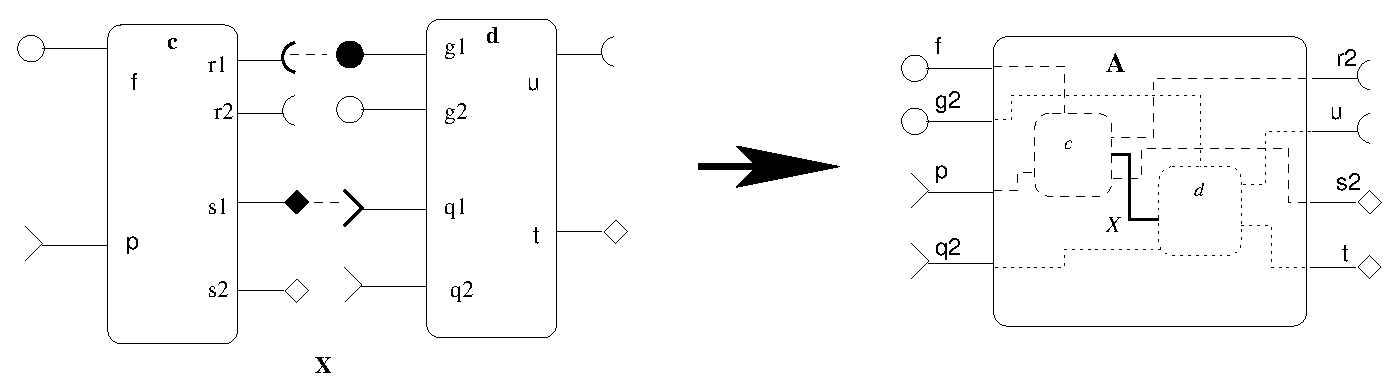
\epsfig{width=.8\textwidth,file=figures/fig-compo-proof.eps}
    \caption{Composition de $c$ et $d$}
    \label{fig-compo-proof}
\end{figure}

\begin{proof}[Composition]
    Nous montrons par induction que tout mot de $L_{\cal A}$ dont les
    pr\'efixes respectent les propri\'et\'es de fiabilit\'e contractuelle et
    d'ind\'ependance des facettes est lui-m\^eme un mot respectant
    ces propri\'et\'es. Autrement dit, si $u$ est un mot de $L_{\cal
    A}$ respectant ces propri\'et\'es, quelque soit la  mani\`ere de
    prolonger ce mot pour obtenir des mots de $L_{\cal A}$, on obtient
    des mots respectant les propri\'et\'es de fiabilit\'e
    contractuelle et d'ind\'ependance des facettes.

\textbf{Si $u=\epsilon$ :}

    Le mot vide $\epsilon$ appartient bien \`a $L_{\cal A}$ et
    trivialement, 
    $\epsilon$ respecte les contrats de chacun des ports de $\cal A$
    par d\'efinition de la propri\'et\'e de relation contractuelle.
    De m\^eme, l'ind\'ependance des facettes est \'evidemment respect\'ee.

\textbf{Si $u\neq\epsilon$ :}

Par hypoth\`ese d'induction :
\begin{itemize}
  \item pour tout port $p\in Port(\cal A)$, $\Pi_{\ialph(p)}(u) \in L_p$ ;
  \item pour toute facette $f\in Port({\cal A})$, l'ind\'ependance de $f$ est respect\'ee. Notons
    $F=\{(f,I,\mathtt{facet}) \in Port({\cal A})\}$ cet ensemble, l'on
    consid\'ere donc que  $u$ est de la forme $u=i_1 u_1o_1 i_2
    u_2 o_2 \dots   i_n u_n o_n$ avec :
    \begin{itemize}
      \item $i_1\in In(\ialph(f))$, $o_1\in Out(\ialph(f))$ pour un
        $f$ non connect\'e quelconque,
      \item et $u_i\in h_X(\ialph({\cal
          A}) \setminus \bigcup_{p\in F}ialph(p))^*$ ;
    \end{itemize}
  \item $u = v \mix x \mix w$
    avec $v \in h_X(\Tr(c))$, $w\in h_X(\Tr(d))$ et $x\in L_X$.
\end{itemize}

    Soit $a\in \ialph({\cal A})$  telle que $ua\in
    L_{\cal A}$. Si $a\in \ialph(p), p\in Port(c)\cup Port(d)\setminus
    Port({\cal A})$, $p$ un port connect\'e de l'assemblage, $ua$ est
    de toute \'evidence contractuellement correct pour les ports de
    $Port({\cal A})$ et il
    suffit donc de consid\'erer les diff\'erentes possibilit\'es de prolonger le
    mot $u$ par une lettre $a\in \ialph(p)$ pour $p\in Port({\cal A})$
    un port non connect\'e de l'assemblage :
    \begin{enumerate}
      \item si $a\in \ialph(p), p\in \Rc(d)\cup \Source(d)\cup \Sink(d)$, par hypoth\'ese de
        fiabilit\'e de $d$, $wa$ est fiable pour $p$ et donc 
        $$
        u'=ua = v\mix x \mix wa
        $$
        est fiable et respecte l'ind\'ependance des facettes ;
      \item si $a\in \ialph(p), p\in \Rc(c)\cup \Source(c)\cup \Sink(c)$, par hypoth\'ese de
        fiabilit\'e de $c$, $va$ est fiable pour $p$ et donc 
        $$
        u'=ua = va\mix x \mix w
        $$
        est fiable et respecte l'ind\'ependance des facettes ;
      \item si $a\in \ialph(f), f\in \Fc(d)$, par hypoth\'ese de
        fiabilit\'e de $d$, $\Pi_{\ialph(f)}(w)i \in \Tr(f) \implies wi \in \Tr(d)$ et il existe $o\in h_c(Out(\ialph(f)))$ tel que
        $wiyo\in \Tr(d)$. Par hypoth\`ese d'ind\'ependance des facettes
        de $d$, $y\in \ialph(d)\setminus
        \cup_{p\in \Fc(d)\cup \Sink(d)}ialph(p))^*$. On a donc  
        $$
        u'= uiyo = v\mix x \mix wiyo
        $$
        est fiable et respecte l'ind\'ependance des facettes de ${\cal A}$.
    \end{enumerate}

    Nous d\'etaillons manintenant le cas o\`u $a$ est une lettre
    d'une facette de $c$.
    Soit $f$ une facette de $c$ et $i\in h_c(In(\ialph(f)))$ tel que
    $ui\in L_{\cal A}$. Par hypoth\`ese de fiabilit\'e de $c$,
    $\Pi_{\ialph(f)}(v)i \in \Tr(f) \implies vi \in \Tr(c)$ et il existe $o\in h_c(Out(\ialph(f)))$ tel que
    $viyo\in \Tr(c)$, avec $y\in h_X(\ialph(c)\setminus
    \cup_{p\in \Fc(c)\cup \Sink(c)}ialph(p))^*$. 
    
    Si $y=\epsilon$, alors 
    $$
    (v \mix x \mix w)io = (vio \mix x \mix w) \subseteq L_{\cal A},
    $$
    donc $L_{\cal A} \sim f$ et trivialement ${\cal A}\perp f$. 
    
    Si $y\neq\epsilon$, alors par hypoth\`ese d'ind\'ependance des
    facettes de $c$, $y\in (\cup_{p\in\Rc(c)\cup
      \Source(c)}\ialph(p))^*$ et par hypoth\`ese de fiabilit\'e de
    $c$ on a
    $$
    y \in (o_1 i_1) \sh (o_2 i_2) \sh \dots \sh (o_n i_n),
    $$ 
    avec 
    \begin{eqnarray}
        o_j \in \ialph(r), \mbox{~pour~} r\in \Rc(c) \implies
        \Pi_{\ialph(r)} (v o_j i_j) \in \Tr(r) \label{eq:c-fiab-rec-ncnx}\\
        \mbox{~et~} \notag\\
        o_j \in \ialph(s), \mbox{~pour~} s\in \Source(c) \implies
        i_j = \epsilon \mbox{~et~} \Pi_{\ialph(s)} (v o_j ) \in
        \Tr(s).\label{eq:c-fiab-puits}
\end{eqnarray}
$y$ est constitu\'e uniquement de messages arbitrairement
    entrelac\'es en fonction du langage de $c$ concernant des
    r\'eceptacles et puits de $c$. 

Soit $I\subseteq \mathbb{N}$ un ensemble d'indices $I$, $I$ est
totalement ordonn\'e par la relation d'ordre naturelle des entiers et
l'on \'ecrira 
$$
\bigodot_{i\in I} u_i
$$
la concat\'enation d'un ensemble de mots indic\'es par des
\'el\'ements de $I$ dans l'ordre induit par cet ensemble : 
$$
\bigodot_{i\in I} u_i = \bigodot_{j=1}^{\vert I\vert} u_{i_j} = u_{i_1} u_{i_2} \dots u_{i_n},  
$$
avec pour tout $i_j,i_k$, $j<k \Leftrightarrow i_j < i_k$.


    Soit $I\subseteq \{1,\dots,n\}$ un \emph{marquage} tel que $\forall j \in I, \exists
    (c,r,d,g)\in X$ tel que $o_j$ et 
    $i_j$ appartiennent \`a $\ialph(r)$, 
    \begin{align*}
        y_d&=\Pi_{\cup_{\ialph(g), (c,r,d,g)\in X}}(y)\\
        &=\bigodot_{j\in I} o_j i_j.
    \end{align*}
    
    Comme $c \sim r$, $d\sim g$ et $d \perp g, \forall g \in \Fc(d)$
    tels que $(c,r,d,g)\in X$, alors pour tout $j\in I$ il existe $z_j$ tel que 
    $$
    w \bigodot_{j\in I} (i_{g_j} z_j o_{g_j}) \in \Tr(d)
    $$ 
    avec $z_j \in h_X(\ialph(d)\setminus \cup_{p\in \Fc(d)\cup
    \Sink(d)}\ialph(p))^*$ et $\Pi_{\ialph(g)}(w i_g o_g) \in \Tr(g),
    \forall g \Fc(d)$. Notons que l'inclusion de la projection dans le
    langage d\'ecoule du fait que $c\sim r$ et que $L_r=
    \bar{h}(L_g)$ donc les sorties produites par $L_c$ sur $r$ sont
    incluses dans l'ensemble de sorties produites par $L_r$, ce qui
    par application de $\bar{h}$ implique que les entr\'ees sur $d$
    par $g$  depuis $r$  sont incluses dans les entr\'ees possibles sur
    $L_g$.
    
    Pour tout $\chi =(c,r,d,g)$, par construction de $L_\chi$, pour
    tout $j\in I$, $x o_j i_{g_j}  o_{g_j} i_j \in L_\chi$ avec
    $i_{g_j}= \bar{h}(o_r),o_{g_j}=\bar{i}_j$. 

    Par ind\'ependance des facettes de $d$, on a
    \begin{align*}
        u' &= (viyo \mix x(\sh_{\{(r,g) \mid (c,r,d,g) \in
          X,\Pi_{\ialph(r)}(y)\neq \epsilon\}} o_r i_g o_g i_r) \mix
        w() \\
        &=(v \mix x  \mix w)i o_1 i_{g_1} z_1 o_{g_1} i_1 . o_2 i_{g_2} z_2
        o_{g_2} i_2  \dots o_k i_{g_k} z_k
        o_{g_k} i_k o.
    \end{align*}
    Comme $\forall i \in \ialph(f), \Pi_{\ialph(f)}(u')i \in L_{\cal
      A}$  et $\Pi_{\ialph(f)}(u')io \in \Tr(f)$, donc  
    $$
    \forall f\in \Fc(c), u' \sim f.
    $$ 
  
  Par hypoth\`ese de fiabilit\'e de $d$, on a bien $\forall j\in I$
  tel que $z_j\neq \epsilon$, pour tout r\'eceptacle et puits $q$
  de $d$, $\Pi_{\ialph(q)}(L_d) \geq L_q$ d'o\`u $\Pi_{\ialph(q)}(w
  z_j) \in L_q$, $\Pi_{\ialph(q)}(u z_j) \in L_q$,  donc  
  $$
  \forall q\in \Rc(d)\cup \Sink(d), u' \sim q.
  $$  
  
  Enfin, en appliquant une construction similaire pour toutes les
  sources de $c$, on d\'eduit 
  $$
  \forall s\in \Source(d)\setminus elem(X), u\sim s \implies u' \sim s.
  $$  

  De m\^eme, pour toutes les facettes non connect\'ees de $d$, par
  hypoth\`ese d'ind\'ependance et de fiabilit\'e, on a 
  $$
  \forall f\in (\Fc(d)\cup \Source(d))\setminus elem(X), u' \sim f.
  $$  

  De \eqref{eq:c-fiab-rec-ncnx} et \eqref{eq:c-fiab-puits} on d\'eduit 
  \begin{align*}
      \forall r\in \Rc(c)\setminus elem(X), u'\sim c&\mbox{~et~}& \forall r\in
      \Sink(c)\setminus elem(X), u'\sim c.
  \end{align*}

  Enfin, en appliquant une construction similaire pour toutes les
  sources de $c$, on d\'eduit 
  $$
  \forall s\in \Source(d)\setminus elem(X), u\sim s \implies u' \sim s.
  $$  
  
  On a donc, pour tout les ports $p$ non connect\'es  de $c$ et $d$,
  $u'\sim p$ donc ${\cal A}$ est fiable pour $Port({\cal A})$ et
  respecte l'ind\'ependance des facettes de $Port({\cal A})$.\hfill\qed
\end{proof}

\subsubsection{Composite}

Pour pouvoir \'etendre ce r\'esultat de mani\`ere inductive d'un assemblage de deux
composants \`a un assemblage de $n$ composants, il est n\'ecessaire
de pouvoir construire un composant \`a partir d'un assemblage. Nous
d\'efinissons donc dans cette section la notion de \emph{composite},
c'est \`a dire de composant form\'e \`a partir d'un assemblage.
Pour ce faire, il faut fournir au nouveau composant 
une identit\'e propre et  veiller \`a ce que les ports non
connect\'es soient correctement renomm\'es, afin d'\'eviter des
collisions de noms avec des ports de m\^eme noms fournis par d'autres
composants participant du m\^eme assemblage.
On obtient ainsi une entit\'e autonome et opaque qui se comporte
comme n'importe quel autre composant. 

\begin{definition}[Composite]
\label{def:composite}
\'Etant donn\'e un assemblage ${\cal A} = \langle B,X\rangle$
\emph{fiable} pour l'ensemble de ses ports non connect\'es
$Port({\cal A})$, on
d\'efinit l'instance de composant $c=\langle P, L_c\rangle$ comme
suit :
\begin{itemize}
  \item $P = \cup_{c_i\in B} \{(c_i^p,T,g)\mid (p,T,g) \in Port({\cal A})\}$ est l'ensemble des ports de $c$ ;
\item $L_c = h_c(L_{\cal A})$ est le langage de $c$ ;
\end{itemize}
avec le morphisme $h_c$ d\'efini comme :
$$\begin{array}{rlcl}
h_c:&\ialph({\cal A}) &\longrightarrow& \ialph(c) \\
&(c_i,p,\gamma_2,\varrho_2,k,m,\vec{x},v)&\longmapsto&(c,c_i^p,\gamma_2,\varrho_2,k,m,\vec{x},v)
\mbox{~si~} (c_i,p) \not\in elem(X)\\
&(\gamma_1,\varrho_1,c_i,p,k,m,\vec{x},v)&\longmapsto&(\gamma_1,\varrho_1,c,c_i^p,k,m,\vec{x},v)
\mbox{~si~} (c_i,p) \not\in elem(X)\\
&x&\longmapsto&\epsilon\mbox{~sinon.}
\end{array}$$
\end{definition}

Classiquement, l'op\'eration d'encapsulation que repr\'esente la
formation d'un composite \`a partir d'un assemblage a pour effet de
supprimer du langage de ce dernier les messages relatifs aux ports
connect\'es. Les ports restant, non connect\'es, sont alors
renomm\'es et l'on obtient une nouvelle instance de composants
d'identit\'e $c$.

\subsubsection{Assemblage fiable}

Une derni\`ere condition pour \'etendre la composition de deux
composants \`a $n$ composants assembl\'es sur un ensemble de
connexions est li\'ee \`a la \emph{topologie } des connexions. 
Pour tout ensemble de connexions $X$, on peut d\'efinir un graphe dirig\'e
$G_X=(S,A)$ o\`u $S$ est l'ensemble des sommets du graphe et $A\subseteq
S\times{}S$ est l'ensemble des arcs du graphe, construit comme suit :
\begin{itemize}
  \item $S = elem(X)$ ;
  \item $A = \{ ((c,p),(c,p')) \mid p\in \Fc(c)\cup\Sink(c)\wedge
  p'\in \Rc(c) \cup \Source(c)\} \cup \{ ((c,p),(c',p')) \mid
  (c,p,c'p')\in X\}$.
\end{itemize}

\begin{definition}[Enesmble de connexions consistant]
\label{def:cnx-consistantes}
Soit $X$ un ensemble de connexions, $X$ est \emph{consistant} si et
seulement si le graphe de connexion induit par $X$, $G_X$, est acyclique.
\end{definition}

\begin{theoreme}[Compositionnalit\'e]
\label{th:compositionnalite}
    Soit ${\cal A} = \langle B,X \rangle$ un assemblage tel que
    l'ensemble $X$ des connexions est \emph{consistant} (d\'efinition
    \ref{def:cnx-consistantes}) et tel que tout composant $c\in B$ est
    \emph{fiable} (d\'efinition \ref{def:fiab-dun-comp}),
    alors ${\cal A}$ est \emph{fiable} pour l'ensemble des ports non
    connect\'es $Prot({\cal A})$.
\end{theoreme}

\begin{proof}
    Le graphe $G_X=(S,A)$ induit par l'ensemble de connexions $X$
    (d\'efinition \ref{def:cnx-consistantes}) \'etant dirig\'e
    acyclique, on peut \'enum\'erer $elem(X)$, l'ensemble des
    sommets de $G_X$, suivant un tri topologique associ\'e \`a
    l'ordre partiel induit par les arcs de $G_X$. D'o\`u 
    $$
    \forall s,s' \in S, s\leq s' \Leftrightarrow 
    \begin{array}{l}
s = s' \\
\mbox{ou~} (s,s')\in A \\
\mbox{ou~} \exists s''\in S, s\leq s'' \mbox{~et~} s''\leq s'.
    \end{array}
    $$
    
    En particulier, si $(c,r,d,f)\in X$, $(c,r)\leq (d,f)$  et par
    acyclicit\'e du graphe, il n'existe pas de ports $p$ dans
    $Port(c)$,$q$ dans $Port(d)$ tels que  $(d,q)\leq (c,p)$. 
    Soit $n=\vert B\vert$, alors l'ordre
    d\'efini ci-dessus induit une \emph{bijection} $\iota:B
    \rightarrow \{1,\dots,n\}B$ qui associe un indice \`a chaque composant. On a
    donc $\iota(c)=\iota(d) \implies c= d$ et 
    $$
    \iota(c)< \iota(d) \implies 
    \forall (c,p,d,q)\in X, p\in \Rc(c)\cup \Source(c) \mbox{~et~} q\in
    \Fc(d)\cup \Sink(d).
    $$

    Par induction sur l'ordre de $\iota$ :
    \begin{itemize}
      \item pour $c$ tel que $\iota(c) = 1$, par hypoth\`ese $c$ est
        fiable et donc ${\cal
          A} = \langle \{c\},\emptyset \rangle$ est fiable ;
      \item soit $k\in \{1,\dots n\}$, on suppose que le composite  ${\cal C}_k$
      produit \`a partir de l'assemblage ${\cal A}_k$  tel que ${\cal A}_k = \langle
      \{\iota^{-1}(1),\dots,\iota^{-1}(k) \}, X_k=\{(c,p,d,q)\mid \iota(c)\leq k
      \mbox{~et~} \iota(d)\leq k\}\rangle$ est fiable. Soit ${\cal
      A}_{k+1}$ l'assemblage d\'efini par ${\cal A}_{k+1} = \langle
      \{{\cal C}_k,\iota^{-1}(k+1)\}, X_{k+1}=\{(c,p,d,q)\in X
      \mid d=\iota^{-1}(k+1)\}\rangle$ :
      \begin{itemize}
        \item si $X_{k+1} = \emptyset$, alors ${\cal A}_{k+1}$ est
        l'union sans connexion de deux composants fiables et par
        cons\'equent est fiable,
      \item sinon, par application du lemme
        \ref{lem:assemblage-de-deux} avec $c={\cal C}_k$ et
        $d=\iota^{-1}(k+1)$, on a bien ${\cal A}_{k+1}$ est fiable ce qui
        termine l'induction.\hfill\qed
      \end{itemize}
    \end{itemize}
\end{proof}

\subsection{Composition \& Mod\`eles}

Nous avons dans les pr\'ec\'edentes sections d\'efini la
composition en termes d'\emph{instances de composants}. On peut tout
aussi bien consid\'erer qu'il est int\'eressant de sp\'ecifier
directement un assemblage. Pour ce faire, nous \'etendons la syntaxe
et la s\'emantique du langage \textsf{FIDL} (voir chapitre
\ref{chap-fidl}). 

La syntaxe --- au niveau \textsf{IDL3} du langage --- de la
d\'efinition d'un \emph{composite}  est d\'ecrite 
par la grammaire dans la figure \ref{fig-syn-fidl-assm}. Elle
introduit un mot-cl\'e $\mathtt{assembly}$  et permet
de d\'ecrire le composite correspondant en nommant les composants qui
le r\'ealisent et en d\'efinissant les connexions entre ces
composants. 
Les lex\`emes $\mathtt{id}$ et $\mathtt{fqname}$ d\'esignent
respectivement un identifiant valide en \textsf{IDL3} et un nom
qualifi\'e.

\begin{figure}
    \begin{equation}
        \label{eq:syn-fidl-assm}\begin{array}{r@{\quad\rightarrow\quad}l}
            Composite & \mathtt{assembly}\ \mathsf{id}\ \mathtt{\{}\
              Assembly\ \mathtt{\} ;} \\
            Assembly & Assembly\ Component \mid Assembly\ Connection 
            \mid Assembly\ Hide\mid \epsilon \\
            Component & \mathtt{component}\ Type\ \mathsf{id}\ \mathtt{;}  \\
            Connection & \mathtt{connection}\ Port\ Port\ \mathtt{;}  \\
            Hide & \mathtt{hide}\ Port\ \mathtt{;}  \\
            Port & \mathsf{id}.\mathsf{id} \\
            Type & \mathtt{fqname}
        \end{array}
    \end{equation}
    \caption{Syntaxe des composites}
    \label{fig-syn-fidl-assm}
\end{figure}

Cette syntaxe permet de d\'efinir un nouveau --- type de ---
composant par assemblage de composants plus primitifs. Les
d\'efinitions relatives aux assemblages (d\'efinition
\ref{def:assemblages}) et aux composites (d\'efinition \ref{def:composite}) doivent
\^etre simplement adapt\'ees : le terme instance de composant
d\'esigne alors simplement un composant nomm\'e de l'assemblage. Les
d\'efinitions de langages et d'alphabets sont identiques. La seule
modification importante concerne le \emph{masquage} de ports ce qui
implique de red\'efinir l'ensemble des ports d'un composite.

\begin{definition}[Masquage de ports]
Soit $C$ un composant et $H\subseteq \Fc(C)\cup \Sink(C)$  un ensemble de ports
\emph{masqu\'es}, alors on d\'efinit le composant $C'=\langle Port(C)
\setminus H,\Tr(C) \rangle$.
\end{definition}

On notera que le langage de $C'$ est identique au langage de $C$. La
suppression des ports masqu\'es  de l'ensemble de ports implique
n\'ecessairement l'impossibilit\'e de se connecter sur les ports
masqu\'es donc l'impossibilit\'e de \og produire \fg{} les mots
induits par un appel ou un message sur une facette ou un puits
masqu\'e. Par ind\'ependance des facettes, on est assur\'e
toutefois de conserver un comportement fiable du composant dont les
ports sont masqu\'es. 

%% \begin{definition}[Composite (2)]
%% \label{def:type-composite}
%%     Un \emph{composite} $\cal C$ est d\'efini par :
%%     \begin{itemize}
%%       \item un ensemble $B$ de couples $(C,n)$ o\`u $C$ identifie un
%%         composant et $n$ est un nom \emph{unique} dans $B$ ;
%%       \item un ensemble de connexions $X$ constitu\'e de quadruplets
%%         $(c,r,d,f)$ o\`u $c,d$ sont des noms d'\'el\'ements de $B$ et
%%         $r$ --- resp. $f$ ---  un  noms de port appartenant respectivement au composant
%%         identifi\'e par $c$ --- resp. $d$.
%%     \end{itemize}
%%     Le langage de l'assemblage $L_{\cal C}$ et son alphabet sont d\'efinis par :
%%     \begin{eqnarray}
%%         \ialph({\cal C}) = \bigcup_{(C,n)\in B}h_X(h_n(\ialph(C))),\label{eq:alph-assemblage} \\
%%         L_{\cal C} = (\bigsh_{(C,n)\in B} h_X(h_n(L_C)))\bigmix_{\ialph({\cal
%%             C}),\ialph(X)} (\bigsh_{\chi \in X} L_\chi). \label{eq:lang-assembly}
%%     \end{eqnarray}
%%     Le morphisme $h_n$ pour un nom de composant $n$ est d\'efini
%%     simplement par 
%%     $$
%%     \begin{array}{rlcl}
%%         h_n:&\ialph({\cal C}) &\longrightarrow& {\cal E} \\
%%         &(\gamma,p,\gamma_2,\varrho_2,k,m,\vec{x},v)&\longmapsto&(n,p,\gamma_2,\varrho_2,k,m,\vec{x},v)\\
%%         &(\gamma_1,\varrho_1,\gamma,p,k,m,\vec{x},v)&\longmapsto&(\gamma_1,\varrho_1,n,p,k,m,\vec{x},v)\\
%%     \end{array}
%%     $$
%% Un composite $\cal C$ est un composant $\langle Port({\cal C}),
%% L_{\cal C}\rangle$ o\`u 
%% $$
%% Port({\cal C}) = \{h_{p}^{C_n}((p,T,g)) \mid (
%% $$
%% \end{definition}


\subsection{V\'erification}
\label{sec:verification}
Dans la section \ref{sec:compositionnalite}, nous avons d\'efini des
propri\'et\'es attendues des composants --- ind\'ependance des
facettes, respect des contrats des ports --- et des assemblages ---
acyclicit\'e du graphe de connexion --- nous permettant de produire
\emph{par construction} des \emph{composites} poss\'edant ces
propri\'et\'es sans qu'il soit n\'ecessaire de red\'emontrer
leur existence. On a ainsi montr\'e que le mod\`ele \textsf{FIDL}
\'etait r\'eellement \emph{compositionnel} pour certaines
propri\'et\'es fondamentales. 

Il reste bien s\^ur \`a v\'erifier que les composants atomiques
utilis\'es dans un assemblage poss\`edent effectivement ces
propri\'et\'es. Dans le cas d'instances concr\`etes de composants,
ce probl\`eme sera \'etudi\'e au chapitre \ref{cha:test}
consacr\'e au test de composants \textsf{FIDL}. Dans le cas 
de \emph{sp\'ecifications} de composants --- simplement appel\'es
\emph{composants}, cette v\'erification doit \^etre r\'ealis\'ee
\`a partir de la sp\'ecification du comportement du composant.

Cette v\'erification rel\`eve \emph{a priori} des techniques de
\emph{v\'erification de mod\`eles} --- \emph{model-checking} en
anglais --- qui constituent un champs de recherche particuli\`erement
actif. Ceci ne rel\`eve toutefois pas du c\oe ur du sujet de cette
th\`ese et nous nous contentons dans cette section d'equisser une
strat\'egie permettant de construire un probl\`eme de model-checking
\`a partir d'un mod\`ele \emph{FIDL} de composant pour v\'erifier
les deux propri\'et\'es n\'ecessaires \`a la compositionnalit\'e
des composants :
\begin{itemize}
  \item l'ind\'ependance des facettes ;
  \item le respect des contrats li\'es aux diff\'erents ports.
\end{itemize}

\subsubsection{Ind\'ependance des facettes}

Le probl\`eme de l'ind\'ependance des facettes est
plus simple que celui du respect des ports. En
effet, on peut transformer la propri\'et\'e
\ref{def:indep-des-facett-1}  d'ind\'ependance sous la forme de l'\'equation
\eqref{eq:prop-independance} : pour toute s\'equence $u$ de messages abstraits
--- voir \'equation \eqref{eq:def-morph-abst} --- du langage du
composant, la projection sur l'union des alphabets abstraits des
facettes et puits du
composant du langage r\'esiduel de $u$ est \'egale au
produit de m\'elange de la projection du langage r\'esiduel de $u$
sur l'alphabet abstrait de chacune de ses facettes 
et puits. 

\begin{prop}
Soit $C=\langle Port(C),\Tr(C) \rangle$ un composant et soit
$\Lambda_C=h_\lambda(\Tr(C))$ le langage associ\'e \`a $C$ sur l'\emph{alphabet
abstrait} des messages. Alors,  $ \forall f \in \Fc(C),C\perp f,$ si et seulement si
\begin{equation}
    \begin{array}{c}
        \forall u \in \Lambda_C, \\
        \prod_{\bigcup_{p\in \Fc(C)\cup \Sink(C)}h_\lambda(\ialph(p))}(u^{-1}\Lambda_C) =
        \bigsh_{p \in \Fc(C) \cup \Sink(C)} \Pi_{h_\lambda(\ialph(p))}(u^{-1}\Lambda_C).
    \end{array}\label{eq:prop-independance}
\end{equation}
\end{prop}
Autrement dit, pour chaque facette et puits du composant, il existe
toujours dans le langage du composant une s\'equence de messages
o\`u n'intervient aucun autre facette ou puits du composant. 

Cette formulation nous permet de travailler pour la v\'erification de cette
propri\'et\'e non pas sur le langage de l'expression de $C$ avec les contraintes sur le contenu des
messages mais uniquement sur les  \emph{enveloppes} des
messages, donc sur un langage reconnaissable par un automate
standard avec un alphabet fini. 

Pour chaque \'etat $q$ d'un automate, le langage associ\'e \`a $q$,
$L_q$, est pr\'ecis\'ement le langage r\'esiduel de $L$ ou quotient
\`a gauche  de $L$ pour tous les mots $u$ tels qu'il existe un chemin
dans l'automate entre $q_0$ et $q$. Il suffit donc de v\'erifier cette
propri\'et\'e pour chaque \'etat $q$ de l'automate associ\'e \`a $\Lambda_C$. 

\subsubsection{Respect des ports}

La v\'erification du respect des ports, et en particulier du respect
des contrats des facettes et r\'eceptacles --- propri\'et\'es
\ref{def:respect-receptacles} et \ref{def:respect-facettes} --- est
nettement plus ardue puisque dans ce cas, il est n\'ecessaire de
prendre en compte les valeurs, contraintes et  fonctions
n\'ecessaires \`a la construction du corps des messages. 
De toute \'evidence, sans hypoth\`ese suppl\'ementaire sur ces \'el\'ements, cette v\'erification est
impossible. 

Un certain nombre de techniques existent pour le \emph{model-checking} de
programmes concurrents, y compris avec des variables. L'approche
introduite dans \cite{smv-thesis} et qui est \`a la base de l'outil
\textsf{SMV} est une des plus connue. Cette approche permet de
g\'erer le probl\`eme de l'explosion du nombre d'\'etats dans
l'analyse d'accessibilit\'e d'un graphe par
l'abstraction d'ensembles d'\'etats sous forme de \emph{Diagrammes de D\'ecision
Binaires}. Une autre approche plus r\'ecente et prometteuse, bas\'ee
sur la \emph{s\'emantique de jeu}, est propos\'ee dans
\cite{abramsky-etal} et d\'etaill\'ee dans \cite{ghica-tg}. Dans une
s\'emantique de jeu\cite{algo-game-sem}, l'ex\'ecution d'un
programme est mod\'elis\'ee comme un \emph{jeu \`a 2 joueurs} entre le
programme et  son environnement. Le principal int\'er\^et de cette
approche est sa compositionnalit\'e qui permet d'interpr\'eter des
fragments de langage comme des \emph{strat\'egies} et de construire une s\'emantique par la
composition des interpr\'etations de ces fragments. Un autre
int\'er\^et est qu'une strat\'egie est d\'efinie comme un langage
rationnel. De notre point de vue, l'utilisation de cette s\'emantique
pr\'esenterait l'int\'er\^et d'unifier dans un m\^eme cadre ---
celui des langages rationnels --- les diff\'erentes parties du
langage \textsf{FIDL}. 

Dans un certain nombre de cas simples, par exemple lorsque les
donn\'ees sont contraintes par des pr\'edicats de base, en l'absence de
fonctions auxiliaires complexes et/ou avec des types de donn\'ees finis, la
v\'erification peut-\^etre faite directement par projection vers un
\emph{model-checker}. 

Le mod\`ele \textsf{FIDL} \'etant bas\'e sur des \emph{automates finis avec
  variables}, on peut  raisonnablement supposer qu'il est
possible d'utiliser les techniques esquiss\'ees ci-dessus pour
  v\'erifier des propri\'et\'es d'un mod\`ele \textsf{FIDL}.

\section{H\'eritage}

\label{sec:heritage-comportemental}
Dans le langage \textsf{FIDL}, les interfaces repr\'esentent des contrats
propos\'es par des composants au travers de facettes et utilis\'es par
ceux-ci au travers de r\'eceptacles. Au niveau purement syntaxique de
l'\textsf{IDL3}, les probl\`emes pos\'es par l'h\'eritage sont extr\^emement r\'eduits,
d'autant plus que le langage n'autorise pas la surcharge de m\'ethodes.
Une interface h\'eritant d'une ou plusieurs autres interfaces \emph{importe}
simplement des m\'ethodes --- signatures --- des super-interfaces et offre une garantie
minimale au client. 

Lorsqu'on s'int\'eresse aux interfaces en tant que sp\'ecification
comportementale des communications entre deux composants au travers de
ports identifi\'es, l'h\'eritage pose divers probl\`emes :
\begin{itemize}
  \item peut-on dans une sous-interface red\'efinir le comportement
    d'une m\'ethode, c'est-\`a-dire changer le contenu des param\`etres attendus en entr\'ee et
    retourn\'es en sortie par la m\'ethode --- bien entendu sans changer
    leur type ?
  \item peut-on \'etendre le comportement d'une super-interface avec
    d'autres m\'ethodes et de quelle mani\`ere ?
  \item peut-on restreindre le comportement d'une super-interface,
    c'est-\`a-dire la sp\'ecialiser et de quelle mani\`ere ?
  \item que se passe-t'il lorsqu'une interface h\'erite de plusieurs
    interfaces d\'efinissant les m\^emes m\'ethodes --- signature identique
    --- mais avec des comportements diff\'erents ?
  \item comment est d\'efini --- et calcul\'e --- l'ensemble de traces
    d'une sous-interface par rapport \`a ses super-interfaces et, corollaire, que
    doit-on r\'e\'ecrire et que peut-on r\'eutiliser ?
\end{itemize}

La relation de sous-typage la plus commun\'ement utilis\'ee
dans le domaine des langages orient\'es objets 
est la notion de \emph{sous-typage comportementale} introduite dans
\cite{liskov94behavioral} et qui s'\'enonce comme suit (traduction
par nos soins) :
\begin{definition}[Sous-typage Comportemental]
Si $\phi(x)$ est une propri\'et\'e prouvable pour tous les  objets $x$ de
type $T$, alors $\phi(y)$ doit \^etre vraie pour tous les objets  $y$ de type
$S$ o\`u  $S$ est un sous-type de $T$.
\end{definition}
Dans le contexte de \cite{liskov94behavioral}, les propri\'et\'es
auxquelles on s'int\'eresse sont des propri\'et\'es de
\emph{s\^uret\'e} : invariants sur l'\'etat (observable) des objets
d'un type et comportement (propri\'et\'es sur l'historique), les
sp\'ecifications \'etant exprim\'ees sous la forme d'assertions
logiques (invariants de type, pr\'e- et post-conditions sur les m\'ethodes).
Ceci revient \`a dire que l'on peut toujours substituer un $y$ pour un
$x$ sans remettre en cause le fonctionnement des \emph{clients} de $x$. 

\subsection{Relation de sous-typage}

On va chercher \`a d\'efinir dans le cadre de sp\'ecifications
\textsf{FIDL} une notion de sous-typage
qui pr\'eserve les propri\'et\'es de compositionnalit\'e des
composants et donc la relation contractuelle existant entre un
fournisseur et un utilisateur d'une interface donn\'ee : pour tout
r\'eceptacle $r$ de type $I$, on doit pouvoir d\'efinir une
connection avec une facette $f$ de type $I$ ou d'un sous-type de (une
interface descendante de) $I$.

Pour ce faire, on va naturellement utiliser la \emph{relation
  contractuelle}  d\'efinie pr\'ec\'edemment (voir d\'efinition
  \ref{def:rel-contrat}). 

\begin{definition}[Sous-typage comportemental]
Soit deux  interfaces $I=\langle meth(I),\Tr(I)\rangle$ et $J=\langle
meth(J),\Tr(J)\rangle$, 
$J$ est un sous-type comportemental de $I$, ce qui est not\'e $I
\sqsubseteq J$ si et seulement si :
\begin{enumerate}
  \item $\ialph(I)\subseteq \ialph(J)$ ;
  \item et $\Tr(I) \lesssim \Tr(J).$
\end{enumerate}
\end{definition} 

Autrement dit, une sous-interface acceptera au moins toutes les
entr\'ees de sa super-interface et produira au plus toute les sorties
qu'aurait produite celle-ci, ce qui correspond aux propri\'et\'es usuelles
d'affaiblissement des pr\'econditions et de renforcement des post-conditions. 
Cette d\'efinition autorise une sous-interface \`a
red\'efinir le comportement de sa super-interface tant que la
transparence est respect\'ee pour les clients de la super-interface

\subsubsection{Types de donn\'ees}

La relation de sous-typage comportemental s'\'etend
naturellement aux types des param\`etres des messages et des valeurs
de retours. Il est alors n\'ecessaire de respecter la contravariance pour
les param\`etres en mode \textbf{in} et la covariance pour les
param\`etres en mode \textbf{out} et les valeurs de retours. Les
param\`etres en mode \textbf{in-out} ne peuvent donc varier. 

Nous supposons l'existence d'une relation de sous-typage sur
l'ensemble des donn\'ees ${\cal D}$ qui peut \^etre simplement la
relation d'inclusion des ensembles en consid\'erant que les types
sont des parties de ${\cal D}$. Pour tout couple de  types $T$ et $S$, $S$ est un
\emph{sous-type} de $T$ si et seulement si ${\cal D}_T\subseteq {\cal D}_S$. 

Soit deux interfaces $I$ et $J$ telles que $J$ est un sous-type de
$I$, et deux m\'ethodes $m_1=T\ m(T_1,\dots,
T_n) \in meth(I)$, $m_2=T'\ m'(T'_1,\dots, T'_n) \in
meth(J)$. Alors, $m_2$ est une
\emph{red\'efinition} valide de $m_1$ pour  la relation de
sous-typage si $m'=m$ et si :
\begin{itemize}
  \item les types des param\`etres en mode \textbf{in} sont plus
  \og larges \fg{} dans $m_2$ : 
$$
\forall T_i, i\leq in(m_1), {\cal D}_{T_i} \subseteq {\cal D}_{T'_i} ;
$$
\item les types des param\`etres en mode \textbf{out} sont plus
  \og larges \fg{} dans $m_1$ : 
$$
\forall T_i, i\geq out(m_1), {\cal D}_{T'_i} \subseteq {\cal D}_{T_i}.
$$

\end{itemize}
Notons que le langage \textsf{IDL} interdit la \emph{surcharge} des
m\'ethodes, c'est \`a dire l'utilisation d'un m\^eme nom pur deux
m\'ethodes diff\'erentes.

\subsubsection{Exceptions}

L'ensemble des exceptions susceptibles d'\^etre lev\'ees par une
m\'ethode $m$ est not\'e $exceptions(m)$. Les messages d'exception
constituent une classe diff\'erentes des appels et des retours de
m\'ethode, mais qui est prise en compte dans le langage de
l'interface. Un appel de m\'ethode et un retour d'exception sont
autoris\'es par les r\`egles de formation des langages d'interfaces
(voir la d\'efinition \ref{def:traces-interfaces}). 

Par cons\'equent, pour deux interfaces $I$ et $J$ avec $I\sqsubset J$
et deux m\'ethodes $m \in meth(I)$, $m'\in meth(J)$, $m'$ est une
red\'efinition valide de $m$ pour la relation de sous-typage si
$exceptions(m') \subseteq exceptions(m)$ : une m\'ethode peut choisir
de lever moins d'exceptions.

\subsection{Sous-typage \& Connexions}

Le principal int\'er\^et de pouvoir d\'efinir une relation de
sous-typage est bien entendu que cette relation s'int\`egre
harmonieusement dans les m\'ecanismes de connexion et de composition
du langage. 
Nous modifions donc la d\'efinition \ref{def:connexions} d'une connexion pour
autoriser la mise en relation de ports dont les types
respectifs appartiennent \`a une relation de sous-typage
comportemental. 

\begin{definition}[Connexion]
Une connexion $\chi$ entre deux ports $(p,I,g)$ et $(p',J,g')$ appartenant respectivement
\`a deux instances de composants $c$ et $c'$ et tels que 
\begin{itemize}
  \item $(g,g') \in \{(\mathtt{receptacle},\mathtt{facet}),(\mathtt{source},\mathtt{sink})\}$
    ;
  \item et $I\sqsubseteq J$ ;
\end{itemize}
est not\'ee $\chi = (c,p,c',p')$. Son alphabet et son langage sont
d\'efinis comme pr\'ec\'edemment (d\'efinition  \ref{def:connexions}).
\end{definition}

\subsection{Substitution de composants}

Du point de vue de la conception d'une architecture \`a base de
composants, une question des plus int\'eressante est de savoir s'il
est possible de remplacer un composant $C$ par un composant $D$. Si le
composant $D$ est le r\'esultat d'un assemblage, on d\'efinit ainsi
un processus de \emph{raffinement} d'architecture. Cette substitution
doit d'une part pr\'eserver la fiabilit\'e du composant
substitu\'e, d'autre part pr\'eserver sa s\'emantique. 

De mani\`ere assez \'evidente, un
composant peut-\^etre substitu\'e \`a un autre composant s'il offre
au moins les m\^emes services. Par contre, il n'est pas requis que le
composant de substitution poss\`ede les m\^emes d\'ependances que le
composant substitu\'e. Si $C$ et $D$ sont des composants fiables,au sens  de
la d\'efinition \ref{def:fiab-dun-comp},
et si l'on substitue $C$ \`a $D$ dans un assemblage fiable,  alors de toute \'evidence
la substitution pr\'eserve la fiabilit\'e. 

Du point de vue de la conception d'une architecture, le  fait de
pr\'eserver la s\'emantique du composant est une propri\'et\'e bien plus
int\'eressante que la simple pr\'eservation de la fiabilit\'e. La
pr\'eservation du langage d'un composant substitu\'e ne peut \^etre
maintenue par la seule d\'efinition de r\`egles de d\'ecomposition
et il est alors  n\'ecessaire de s'int\'eresser au langage du composant de
substitution 
et de s'assurer de sa \og conformit\'e \fg{} avec celui du composant
qui est remplac\'e. 
Cette probl\'ematique sort du cadre strict de ce travail et
constituera un axe de recherche ult\'erieur.

\section{Conclusion}

Le mod\'ele que nous avons defini pr\'esente un certain nombre de
caract\'eristiques int\'eressantes pour raisonner sur des
architectures de composants ouvertes. Le fait qu'il soit bas\'e
int\'egralement sur des langages et des op\'erations pr\'eservant
la rationnalit\'e des langages --- morphismes, produits de
synchronisation et de m\'elange, intersections, ... --- nous permet,
dans le cas o\`u les types de donn\'ees transport\'ees par les
messages sont finis, de raisonner avec des outils classiques tels que
des \emph{contr\^oleurs de mod\`eles} sur des mod\`eles
arbitrairement complexes.
La structure particuli\`ere de l'alphabet nous permet de travailler
\`a diff\'erents niveaux de composition avec les m\^emes
m\'ethodes et raisonnement et surtout nous permet de choisir le
niveau de d\'etail auquel on souhaite s'int\'er\'esser. 

La propri\'et\'e de fiabilit\'e des composants dont nous avons
montr\'e qu'elle \'etait pr\'eserv\'ee par la composition
moyennant certaines restrictions sur la topologie des connexions  est
int\'eressante car elle permet dans un grand nombre de cas et en
particulier dans celui du test de composants, de se
passer d'une v\'erification globale d'un syst\`eme r\'ealis\'e par
assemblage de plusieurs composants. Cette possibilit\'e peut \^etre
particuli\`erement utile pour le raisonnement dans les probl\`emes
d'adaptation ou de substitution d'architectures de composants.

%%% Local Variables: 
%%% mode: latex
%%% TeX-master: "these"
%%% End: 

\chapter{Test de composants FIDL}
\label{cha:test}
\lstset{basicstyle=\footnotesize\sffamily,language=Java,moreemph={end},emphstyle=\bfseries,commentstyle=\itshape,frame=single}

Le mod\`ele d'architecture de composants que nous avons
d\'etaill\'e dans les chapitres pr\'ec\'edents s'appuie sur une
s\'emantique exprim\'ee en termes d'automates dont les alphabets
distinguent les entr\'ees et les sorties. Nous avons vu dans le chapitre
\ref{chap-etatarttest} que cette cat\'egorie de syst\`eme
constituait les bases d'une th\'eorie  du test de protocoles de
communication. L'objectif de ce chapitre est de montrer comment cette
th\'eorie du test d'\textsf{IOLTS} peut \^etre utilis\'ee pour
tester la conformit\'e d'une implantation d'un composant par rapport
\`a une sp\'ecification. 

Si ses principes de base  peuvent \^etre
directement appliqu\'es, les algorithmes utilis\'es n\'ecessitent
d'\^etre adapt\'es au mod\`ele particulier que nous avons
d\'efini. Le probl\`eme principal auquel nous sommes confront\'e
est celui de la fragmentation de la sp\'ecification qui se
pr\'esente comme une collection d'automates synchronis\'es. Un
deuxi\`eme probl\`eme est celui de la multiplicit\'e des ports de
communication et du parall\'elisme intrins\`eque des composants
mod\'elis\'es. Enfin, la notion m\^eme de conformit\'e ne peut
\^etre directement transpos\'ee.

La premi\`ere partie de ce chapitre pr\'esente un algorithme de base
s\'equentiel pour le test de composants mod\`elis\'es comme des
\textsf{IOLTS} qui est une synth\`ese de plusieurs algorithmes
de la litt\'erature. \`A partir de cet algorithme, nous
d\'efinissons plus pr\'ecis\`ement ce que l'on entend par la notion
de conformit\'e d'un composant et les probl\`emes sp\'ecifiques
pos\'es par sa v\'erification au moyen du test. Nous proposons enfin
un processus de test int\'egrant ces diff\'erents
\'el\'ements et permettant la validation par le test de composants
concrets par rapport \`a une sp\'ecification \textsf{FIDL}.

\section{Cadre g\'en\'eral}

Nous d\'efinissons dans cette section le cadre g\'en\'eral pour le
test de composants \textsf{FIDL} \`a partir des travaux sur le test de
portocole \'etudi\'es dans le chapitre \ref{chap-etatarttest}
cosacr\'e \`a l'\'etat de l'art sur le test de conformit\'e. Notre
objectif est d'identifier les probl\`emes pos\'es par le test de
conformit\'e de composants et les principales strat\'egies
permettant de r\'esoudre ces probl\`emes et de s'assurer de la
conformit\'e d'un composants eu \'egard \`a sa sp\'ecification.

\subsection{Rappels}

La th\'eorie du test de conformit\'e d'automates \`a
entr\'ees/sorties est bas\'ee sur les principes du \emph{contr\^ole
  de mod\`ele} entre l'implantation $\cal I$ et le testeur --- ou
observateur --- $\cal O$. Informellement,  on peut mod\'eliser
$\cal I$ et $\cal O$ comme \'etant deux
langages sur un alphabet partitionn\'e en ensembles disjoints de
lettres --- ou actions, ou messages --- d\'enotant soit une
entr\'ee, soit une sortie, soit une action interne. 

La structure de
$\cal I$ \'etant inconnue, le processus de test est alors 
le calcul d'un  \emph{produit de synchronisation} ${\cal I} \| {\cal
  O}$. Dans un mod\'ele de communication \emph{synchrone}, chaque lettre de
sortie de $\cal O$ se synchronise avec une lettre d'entr\'ee de $\cal
I$ et vice-versa. Dans un mod\`ele de communication \emph{asynchrone}, on
introduit un ou plusieurs langages suppl\'ementaires mod\'elisant une \emph{file de
messages}, born\'ee ou non, permettant \`a chacun des deux
langages de se synchroniser avec les files de messages de mani\`ere
ind\'ependante. 

Le test est consid\'er\'e comme r\'eussi si le langage r\'esultant
du calcul du produit de synchronisation ${\cal I} \| {\cal O}$ est dans
une certaine \emph{relation de conformit\'e} avec un langage de
r\'ef\'erence, la sp\'ecification $\cal S$. De fait, l'observateur
${\cal O}$ est construit en fonction de cette relation. 

Si l'observateur est un \emph{langage}, alors son pouvoir
d'observation est au mieux celui de l'\'equivalence entre les
langages ou \'equivalence de traces. Si l'observateur est un automate
ou plus g\'en\'eralement un syst\`eme de transition, alors des
\'equivalences plus fines peuvent \'eventuellement \^etre
observ\'es, li\'ees \`a la structure du graphe de transitions.

 

\subsection{Test d'\textsf{IOLTS}}

L'algorithme g\'en\'erique de test pour la relation de conformit\'e
\textbf{ioco} est introduit dans \cite{tgenioq}. Cet algorithme
pr\'esente la caract\'eristique d'\^etre sain et fiable : il
d\'etecte toutes les implantations erron\'ees et en rejette pas les
implantations conformes. Il produit une suite de test
\emph{compl\`ete} au sens de \cite{itu-z500}. Son principal inconv\'enient est que si le
comportement sp\'ecifi\'e de l'\textsf{IUT} est infini, l'algorithme
ne se termine pas et produit un ensemble de tests infini. 

Il est donc \'evident que dans le cadre d'un processus de test
concret, il est n\'ecessaire de restreindre le test \`a une partie
finie du comportement sp\'ecifi\'e. Cette restriction est
n\'ecessairement bas\'ee sur des m\'ethodes heuristiques
d\'ependant de la connaissance sp\'ecifique du testeur et des
objectifs du processus de test. Toute m\'ethode heuristique se
ram\`ene \emph{in fine} \`a valoriser certains comportements
possibles par rapport \`a d'autres, que ce soit sous la forme d'un
\emph{objectif de test}\cite{tgv,itu-z500,test-pf} ou d'un crit\`ere de couverture inspir\'e
des pratiques du test structurel
\cite{pyhala-test-selection,kervinen-heuristic,curgus-analytic-test,feijs-trace-distance}. 

La figure \ref{fig-algo-test-base} pr\'esente les bases d'un
algorithme, inspir\'e de \cite{pyhala-test-selection},  permettant de v\'erifier la conformit\'e d'une
\textsf{IUT} dont le comportement est suppos\'e \^etre un \textsf{IOLTS} par
rapport \`a une sp\'ecification.  Les param\`etre d'entr\'ee sont :
 \begin{itemize}
   \item une sp\'ecification $S$ sous la forme d'un automate
     \textsf{FIDL} ;
   \item une implantation a tester $I$ suppos\'ee compatible avec $S$,
     c'est \`a dire poss\'edant un alphabet compl\'ementaire et
     disposant d'une op\'eration \textsf{reset} correctement implant\'ee.
 \end{itemize}

Les fonctions auxiliaires non d\'etaill\'ees sont d\'efinies comme :
\begin{itemize}
  \item la fonction \textsf{output(I)} attend une sortie de la part de
    l'\textsf{IUT}, la variable \textsf{out} contenant le r\'esultat
    de la sortie qui peut \'eventuellement \^etre l'observation d'un
    blocage $\theta$ ;
  \item la fonction \textsf{input(I,action)} g\'en\`ere une
  entr\'ee vers l'\textsf{IUT} et retourne \textbf{false} si l'action
  est refus\'ee par l'\textsf{IUT}.
\end{itemize}
L'algorithme de test collecte les traces ayant g\'en\'er\'e des
erreurs dans la variable \textsf{failures}.

\begin{figure}[htbp]
    \centering
 \begin{lstlisting}[linewidth=\textwidth,mathescape=true,numbers=left,numberstyle=\tiny,literate={:=}{{$\leftarrow$}}1 ]
 Input : $S=(Q,q_0,\Sigma,\delta)$           
         $I$           
 Output : failures     
 T := $\emptyset$
 Trace := $\epsilon$ 
 State := $q_0$ 
 Failures := $\emptyset$
 while true 
    //  select an action 
    action := select(S,State,T,Trace)
    switch action
       case terminate: 
           return Failures
       case reset:
           T := T $\cup \{\mathsf{Trace}\}$
           State := $q_0$
           Trace := $\epsilon$
           break
       case output: 
           out := output(I) 
           if out != $\theta$ then
              Trace := Trace.out
              //  unexpected output 
              if out $\not\in$ actions then 
                 Failures := Failures $\cup$ Trace
                 T := T $\cup \{\mathsf{Trace}\}$
                 State := $q_0$
                 Trace := $\epsilon$
              else 
                 State := fire(out)
              end
           else 
              //  a deadlock  
              Trace := Trace.$\theta$
              Failures := Failures $\cup$ Trace
              T := T $\cup \{\mathsf{Trace}\}$
              State := $q_0$
              Trace := $\epsilon$
           end
           break
       default:
          //  select an input 
          if ! input(I,action) 
              //  refused input 
              Trace := Trace.$\theta$
              Failures := Failures $\cup$ Trace
              T := T $\cup \{\mathsf{Trace}\}$
              State := $q_0$
              Trace := $\epsilon$
          else
              Trace := Trace.action
              State := fire(S,action)
          end
       end
 end
 \end{lstlisting}
 \caption{Algorithme de test s\'equentiel}
 \label{fig-algo-test-base}
 \end{figure}

Le c\oe ur de l'algorrithme est constitu\'e de la fonction
\textsf{select} qui comme son nom  l'indique s\'electionne la
prochaine action parmi toutes les actions possibles dans
l'\'etat courant. Cette fonction est d\'etaill\'ee dans
l'algorithme de la figure \ref{fig-algo-select}. 
Elle  effectue le choix de l'action \`a effectuer  en fonction de l'\'etat
courant, de l'ensemble de test g\'en\'er\'e et de la trace de test
courante. Ce choix peut-\^etre :
\begin{itemize}
  \item \textsf{terminate} : le processus de test se termine car
  l'objectif fix\'e est atteint ;
\item \textsf{reset} : l'\textsf{IUT} doit \^etre replac\'ee dans
  son \'etat initial et une nouvelle s\'equence de test est
  construite ;
\item \textsf{output} : le testeur attend une sortie de la part de
  l'\textsf{IUT}. Le message pr\'ecis n'est pas sp\'ecifi\'e ce qui
  autorise les comportements non-d\'eterministes ;
\item $a\in In(Sigma)$ : le testeur doit g\'en\'erer une entr\'e
  sp\'ecifique vers l'\textsf{IUT}.
\end{itemize}

Le choix de ces diff\'erentes actions est subordonn\'e aux deux
fonctions \textsf{objectifAtteint} et \textsf{evaluation}. La
premi\`ere d\'ecide si l'objectif global du processus de test est
atteint et donc l'arr\^ete, la seconde \'evalue les diff\'erentes
actions possibles dans l'\'etat courant en fonction des tests
d\'ej\`a r\'ealis\'es et bien s\^ur des crit\`eres heuristiques
propres au processus du test courant. Notons que dans tous les
\'etats, l'\'evaluation des actions possibles dans cette \'etat est
compar\'ee aux actions possibles depuis l'\'etat initial ce qui
introduit la possibilit\'e de choisir un \textsf{reset}.

Le principal probl\`eme dans le choix des actions \`a effectuer est
celui de la prise en compte du non-d\'eterminisme de la
sp\'ecification qui peut prendre deux formes : 
\begin{itemize}
  \item dans un m\^eme \'etat, des sorties et des entr\'ees sont
    possibles ;
  \item dans un m\^eme \'etat, plusieurs sorties diff\'erentes sont possibles,
\end{itemize}
ces deux formes pouvant bien s\^ur se combiner. Plusieurs solutions
sont envisag\'ees dans la litt\'erature, soit au travers
d'hypoth\`eses quant aux probabilit\'es de telle ou telle action de
sortie, soit plus simplement par un choix al\'eatoire dans le
deuxi\`eme cas d'ind\'eterminisme.
L'\'evaluation que nous pr\'esentons ici tend \`a favoriser les
entr\'ees sur les sorties dans la mesure o\`u sont compar\'es le
maximum de la valorisation des entr\'ees avec le minimum de la
valorisation des sorties. 


\begin{figure}[htbp]
    \centering
    \begin{lstlisting}[linewidth=\textwidth,mathescape=true,numbers=left,numberstyle=\tiny,literate={:=}{{$\leftarrow$}}1 ]
 function select(S,q,T,Trace)
 Input : $S=(Q,q_0,\Sigma,\delta)$
         $q\in Q$
         $T \subset L_S$ 
         Trace $\in L_S$ 
 Output : 
         action $\in \{\mathsf{terminate}, \mathsf{reset}, \mathsf{output}\} \cup In(\Sigma)$

 if objectifAtteint(T,S)  
     action := $\mathsf{terminate}$
 else 
     action := reset
     evalin := $\{ (a,eval(S,Trace.a,T)) \mid (q,a,q')\in \delta, a\in In(\Sigma)\}$
     evalout := $\{ (a,eval(S,Trace.a,T)) \mid (q,a,q')\in \delta, a\in Out(\Sigma)\}$
     evalreset := $\{ (a,eval(S,a,T)) \mid (q_0,a,q')\in \delta\}$
     if max(evalin) < min(evalout) 
       action := output
     else if max(evalreset) > max(evalin)
       action := reset
     else 
       action := max(evalin)
 end
 return action
 \end{lstlisting}
 \caption{Fonction de s\'election}
 \label{fig-algo-select}
 \end{figure}

Bien \'evidemment, nous n'avons encore rien dit sur la fonction
d'\'evaluation elle-m\^eme ni sur la fonction d\'eterminant
l'atteinte de l'objectif du test qui en est un cas particulier. 

\subsubsection{\'Evaluation}

La fonction d'\'evaluation des \'etats ou des actions possibles est
param\'etr\'ee par la sp\'ecification $S$, l'ensemble des tests
d\'ej\`a r\'ealis\'es not\'e $T$ et la s\'equence de test
courante comprenant l'action choisie. Cette fonction est fortement
li\'ee \`a la celle d'\'evaluation d'atteinte de l'objectif  dans
la mesure o\`u elle doit valoriser les actions concourrant \`a
rapprocher l'objectif plut\^ot que les autres.

Cette fonction est bas\'ee sur des crit\`eres heuristiques dont la
justification r\'eside \emph{in fine} dans le choix d'une
strat\'egie de test et d'un mod\`ele de faute. Parmi la faune de
crit\`eres existant, on trouvera : 
\begin{itemize}
  \item la s\'election d'un sous-ensemble fini du comportement de la
    sp\'ecification (objectif de test). La fonction d'\'evaluation
    s\'electionne les entr\'ees en fonction de leur appartenance ou
    non \`a l'objectif de test et la fonction \textsf{objectifAtteint}
    retourne vrai si l'ensemble du comportement d\'efini dans
    l'objectif de test est r\'ealis\'e ;
  \item la s\'election en fonction d'une notion de
    distance sur les s\'equences de
    test. L'existence d'une m\'etrique sur les mots de la
    sp\'ecification dans un espace continu et born\'e permet de
    d\'efinir une notion de couverture \`a partir de la notion de
    limite. La fonction d'\'evaluation va donc favoriser les actions
    am\'eliorant la couverture et le processus s'arr\^ete lorsqu'un
    certain taux de couverture est atteint ;
  \item la s\'election en fonction de divers crit\`eres de
  couverture du graphe sous-jacent au syst\`eme de transition
  sp\'ecifi\'e : couverture des transitions, des \'etats, des paires de
  transitions, ... La fonction d'\'evaluation comme
  pr\'ec\'edemment valorise les actions permettant d'am\'eliorer la
  couverture.
\end{itemize}

Intuitivement, on voit bien que cette fonction d'\'evaluation ne peut
se restreindre \`a prendre des d\'ecisions uniquement en fonction de
l'\'etat courant. Dans le cas contraire, elle court le risque de se
retrouver \og pi\'eg\'ee \fg{} dans des cycles locaux. Il est donc
n\'ecessaire que cette \'evaluation soit r\'ealis\'ee jusqu'\`a
une certaine profondeur dans le graphe sous-jacent et selon des
techniques classiques issues de l'intelligence artificielle :
recherche par branchement-\'elagage, plus court chemin ($A^*$),
minimax, ...

\subsection{Conformit\'e}

Dans le cadre des protocoles
mod\'elis\'es par des syst\`emes de transitions \`a
entr\'ees-sorties, la relation \textbf{ioco} est la plus
fr\'equemment utilis\'ee : sous hypoth\`ese que l'implantation
soit toujours r\'eceptive aux entr\'ees, cette relation
d\'efinie la conformit\'e comme une inclusion des sorties
effectives de l'implantation dans les sorties permises par la
sp\'ecification, et ce pour toute trace valide de cette derni\`ere.

Dans le cas de composants FIDL, l'hypoth\`ese de r\'eceptivit\'e
permanente du composant \`a toutes les entr\'ees possibles ne
correspond pas \`a la r\'ealit\'e des objets que nous cherchons
\`a valider et tester : les facettes et r\'eceptacles mod\'elisent
des \emph{\'echanges} de messages alternant entr\'ees et
sorties. Les ports asynchrones poss\`edent cette propri\'et\'e de
devoir accepter tous les messages mais ici les interactions sont
asym\'etriques et un port ne eut \^etre utilis\'e que danas un seul
mode. 

De plus, la  notion de \emph{contrat} est
essentielle \`a l'architecture de composants que nous avons d\'efini.
Nous utiliserons donc comme relation de conformit\'e la relation
contractuelle d\'efinie au chapitre \ref{cha:composition} d\'efinie  en termes de langages bien-form\'es
(voir d\'efinition \ref{def:langwf}), c'est \`a dire pour lesquels
chaque r\'eception de message est pr\'ec\'ed\'e d'une \'emission. 

On a donc une premi\`ere notion de conformit\'e qui est : 
\begin{quote}
    Un composant est conforme \`a sa sp\'ecification si son
    comportement observ\'e sur chacun de ses ports est conforme
    \`a la sp\'ecification des interfaces typant ces ports.
\end{quote}
Cett premi\`ere conformit\'e nous permet d'envisager de tester
ind\'ependamment chacun des ports du composant pour pouvoir conclure
de sa conformit\'e.

Mais le composant peut poss\'eder lui m\^eme une sp\'ecification,
sous la forme d'un ou de plusieurs automates \textsf{FIDL} 
synchronis\'es. Cette sp\'ecification a pour effet de lier le
comportement des diff\'erents ports du composant entre
eux et de mani\`ere g\'en\'eral de restreindre le comportement
observable sur les diff\'erents ports et de le rendre plus
d\'eterministe que ne l'est la sp\'ecification du port concern\'e :
c'est le sens de la relation contractuelle.

On a donc une notion de conformit\'e plus g\'en\'erale qui est : 
\begin{quote}
    Un composant est conforme \`a sa sp\'ecification s'il est
    conforme \`a la sp\'ecification de chacun de ses ports
    \emph{restreinte} par la sp\'ecification propre du composant.
\end{quote}
Cette deuxi\`eme conformit\'e n\'ecessite de prendre en compte le
comportement sp\'ecifi\'e du composant lors du test de chacun de ses
ports. 

\subsubsection{Test \& automates synchronis\'es}

L'algorithme que nous avons pr\'esent\'e dans la section
pr\'ec\'edente est adapt\'e au cas o\`u l'on teste un \textsf{IUT}
par rapport \`a une sp\'ecification repr\'esent\'ee par \emph{un}
syst\`eme de transition. Or de toute \'evidence, dans le cas de
composants \textsf{FIDL} on se trouve confront\'e au probl\`eme de
construire le produit de synchronisation des
diff\'erents automates qui le compose. M\^eme en se restreignant
\`a des sp\'ecifications sans donn\'ees ou avec des donn\'ees
de types finis, la construction effective de l'automate d\'enotant le
comportement du composant est probl\'ematique. On notera que dans
la plupart des travaux concernant le test de composants multiports ou de
processus concurrents communiquants, ce probl\`eme est suppos\'e
\^etre r\'esolu : on teste une implantation, \'eventuellement
susecptible de communiquer au travers de plusieurs canaux, par rapport
\`a une sp\'ecification globale. 

Pour contourner cette
difficult\'e, il sera donc n\'ecessaire dans le processus de test de
r\'ealiser un synchronisation locale en fonction des besoins de
progression du test. Cette synchronisation locale a des
cons\'equences importantes sur les conclusions que l'on peut tirer
du test en mati\`ee de couverture. En particulier, elle rend
impossible toute mesure de la couverture globale du comportement du
composant. Ce qui implique que la fonction d'\'evaluation du choix
des transitions et le crit\`ere d'atteinte de l'objectif de test ne
peuvent non plus \^etre d\'efinis globalement. 

On va donc distinguer en fonction deux approches de la conformit\'e
et partant deux strat\'egies de test diff\'erentes :
\begin{itemize}
  \item la premi\`ere approche correspond \`a la v\'erification de
  la conformit\'e vis \`a vis des sp\'ecifications des interfaces
  du composantt ;
\item la seconde \`a la v\'erification de la conformit\'e par
  rapport \`a la sp\'ecification du composant (lorsque celle-ci est
  pr\'ecis\'ee).
\end{itemize}
Dans les deux cas, on sera amen\'e \`a synchroniser un ensemble
d'automates \textsf{FIDL} pour d\'eterminer les prochaines actions
\`a effectuer. Mais dans le premier cas, le crit\`ere
d'\'evaluation des actions et de d\'ecision d'arr\^et sera
fonction de la sp\'ecification d'un port synchrone, tandis que dans
le second il sera fonction des automates formant la sp\'ecification
du composant.

\begin{prop}
\label{prop:mix-contrat}
    Soit $L_1$ et $L_2$ deux langages bien form\'es (d\'efinition
    \ref{def:langwf}), soit ${\cal L} = L_1 \mix_{\Sigma_1,\Sigma_2} L_2$ le
    langage r\'esultant du produit de synchronisation de $L_1$ et
    $L_2$, et soit $\cal I$ un
    langage tel que $\ialph({\cal I}) =\ialph({\cal L}).$ 

Alors, 
\begin{gather}    
\label{eq:mix-contrat1}    \Pi_{\Sigma_1}({\cal L}) \lesssim
\Pi_{\Sigma_1}({\cal I}) \wedge
 \Pi_{\Sigma_2}({\cal L})\lesssim \Pi_{\Sigma_2}({\cal I}) \\
\notag    \Leftrightarrow \\
\label{eq:mix-contrat2} {\cal L}\lesssim {\cal I}.
\end{gather}
\end{prop}

\begin{proof}
(\ref{eq:mix-contrat1}) $\implies$ (\ref{eq:mix-contrat2})

Si $\Pi_{\Sigma1}({\cal L})\lesssim \Pi_{\Sigma_1}({\cal I}) \wedge \Pi_{\Sigma_2}({\cal L})\lesssim
\Pi_{\Sigma_2}({\cal I})$, alors il existe deux relations $S_1\subseteq
(\Pi_{\Sigma_1}({\cal I})\times{}\Pi_{\Sigma1}({\cal L}))$ et $S_2\subseteq
(\Pi_{\Sigma_2}({\cal I})\times{}\Pi_{\Sigma1}({\cal L}))$ telles que, si $(u,u)\in S_1$  :
\begin{itemize}
  \item s'il existe $i\in In(\Sigma_1)$ tel que $ui\in \Pi_{\Sigma1}({\cal L})$, alors
    $ui\in \Pi_{\Sigma_1}({\cal I})$ et $(ui,ui)\in S_1$ ;
  \item s'il existe $o\in Out(\Sigma_1)$ tel que $uo\in {\cal I}$, alors
    $uo\in \Pi_{\Sigma1}({\cal L})$ et $(uo,uo)\in S_1$ ;
\end{itemize}
et $(\epsilon, \epsilon)\in S_1$. De m\^eme pour $S_2$. 

Soit $S=\{(u,u)\in ({\cal L}\cap {\cal I}) \mid (\Pi_{\Sigma_1}(u),\Pi_{\Sigma_1}(u)) \in S_1
\mbox{~et~} (\Pi_{\Sigma_2}(u),\Pi_{\Sigma_2}(u))\in S_2\}$, une
relation entre $\cal L$ et $\cal I$, nous montrons que $S$ est une
relation contractuelle. 
Soit $u \in {\cal L}$ tel que $(u,u)\in S$, alors :
\begin{enumerate}
  \item soit $i \in In({\cal L})$ tel que $ui \in {\cal L}$, 
    \begin{itemize}
      \item si $i \in \Sigma_1\cap \Sigma_2$, alors
      $v_1=\Pi_{\Sigma_1}(ui)=\Pi_{\Sigma_1}(u)i \in \Pi_{\Sigma1}({\cal L})$ et
      $v_2=\Pi_{\Sigma_2}(ui)=\Pi_{\Sigma_2}(u)i\in \Pi_{\Sigma_2}({\cal L})$ donc
      $(v_1,v_1)\in S_1$ et $(v_2,v_2)\in S_2$, d'o\`u $(ui,ui)\in S$
      ;
    \item si $i\in \Sigma_1$ et $i\not\in \Sigma_2$, alors
    $v_1=\Pi_{\Sigma_1}(ui)=\Pi_{\Sigma_1}(u)i \in \Pi_{\Sigma1}({\cal L})$ et
    $v_2=\Pi_{\Sigma_2}(ui)=\Pi_{\Sigma_2}(u) \in \Pi_{\Sigma_2}({\cal L})$. On a donc
    $(v_1,v_1)\in S_1$ et $(v_2,v_2)\in S_2$, d'o\`u $(ui,ui)\in S$ ;
  \item si $i\not\in \Sigma_1$ et $i\in \Sigma_2$, l'argument est
  inedntique et l'on en d\'eduit  $(ui,ui)\in S$.
    \end{itemize}
  \item soit $o\in Out({\cal L})$ tel que $uo\in {\cal I}$, on montre
  de la m\^eme mani\`ere que $(uo,uo)\in S$.
\end{enumerate}
Par cons\'equent $S$ est bien une relation contractuelle et comme
$(\epsilon,\epsilon)\in S$ par construction, on en conclut que ${\cal
  L} \lesssim {\cal I}$.

(\ref{eq:mix-contrat2}) $\implies$ (\ref{eq:mix-contrat1})

Si ${\cal L}\lesssim {\cal I}$, alors il existe une  relation $S\subseteq
({\cal I}\times{}{\cal L})$ telle que, si $(u,u)\in S$  :
\begin{itemize}
  \item s'il existe $i\in In({\cal L})$ tel que $ui\in {\cal L}$, alors
    $ui\in {\cal I}$ et $(ui,ui)\in S$ ;
  \item s'il existe $o\in Out({\cal L})$ tel que $uo\in {\cal I}$, alors
    $uo\in {\cal L}$ et $(uo,uo)\in S$ ;
\end{itemize}
et $(\epsilon, \epsilon)\in S$.

Soit $S_1=\Pi_{\Sigma_1}(S)$, nous montrons que $S_1$ est une relation
contractuelle contenant $(\epsilon,\epsilon)$. Soit $u$ tel que
$(u,u)\in S$ et $u_1= \Pi_{\Sigma_1}(u)$, par construction de $S_1$,
$(u_1,u_1)\in S_1$, et de m\^eme :
\begin{enumerate}
  \item soit $i \in In({\cal L})$ tel que $(ui,ui)\in S$, si $i\in
  \Sigma_1$, $u_1i\in \Pi_{\Sigma1}({\cal L})$ et comme $ui\in {\cal I}$, on a bien $u_1i
  \in \Pi_{\Sigma_1}({\cal I})$ et  $(u_1i,u_1i)\in S_1$ ;
  \item soit $o \in Out({\cal L})$ tel que $(uo,uo)\in S$, alors $uo \in
  {\cal I}$ et $uo \in {\cal L}$. Si $o\in \Sigma_1$, il vient $u_1o
  \in \Pi_{\Sigma_1}({\cal I})$,  $u_1o\in
  \Pi_{\Sigma1}({\cal L})$ et $(u_1o,u_1o)\in S_1$.
\end{enumerate}
Donc $S_1$ est bien une relation contractuelle incluse dans
$(\Pi_{\Sigma_1}(I)\times{}\Pi_{\Sigma1}({\cal L}))$ et comme $(\Pi_{\Sigma_1}(\epsilon) =
\epsilon$, $(\epsilon,\epsilon)\in S_1$, d'o\`u l'on conclut que
$\Pi_{\Sigma1}({\cal L})\lesssim \Pi_{\Sigma_1}(I)$. Par un argument indentique on conclut
que $\Pi_{\Sigma_2}({\cal L})\lesssim \Pi_{\Sigma_2}(I)$ ce qui termine la d\'emonstration.\hfill\qed

\end{proof}

Le produit de synchronisation \'etant associatif et commutatif, on
\'etend imm\'ediatement ce r\'esultat \`a un nombre quelconque
d'automates synchronis\'es. 

\begin{prop}[Composition des relations contractuelles]
Soit $${\cal L} = L_1\mix_{\Sigma_1,\Sigma_2} L_2
\mix_{\Sigma_2,\Sigma_3} \dots \mix_{\Sigma_{n-1},\Sigma_n} L_n$$ un
langage mix\'e et soit ${\cal I}$ un autre langage, 
\begin{gather*}    
\bigwedge_{i=1}^n \Pi_{\Sigma_i}({\cal L})\lesssim \Pi_{\Sigma_i}({\cal I}) \\
    \Leftrightarrow \\
{\cal L}\lesssim I.
\end{gather*}
\end{prop}

\begin{proof}
    Imm\'ediate par la proposition \ref{prop:mix-contrat} et les
    propri\'et\'es du produit de synchronisation (d\'efinition
    (\ref{eq:def-mix}). \hfill\qed
\end{proof}

Par cons\'equent, pour v\'erifier qu'un
composant est contractuellement correct pour l'ensemble de ses ports,
il suffit de le v\'erifier pour chacun d'entre eux s\'epar\'ement
en ne tenant compte que de la partie du langage associ\'e \`a ce
port qui se synchronise avec les autres ports et sp\'ecifications du
composant. Autrement dit, la v\'erification est faite sur la
projection du langage du composant sur l'alphabet du port
consid\'er\'e. 
 
De m\^eme. pour v\'erifier que le comportement d'un
composant est conforme \`a sa sp\'ecification, il suffit de
v\'erifier la propri\'et\'e de fiabilit\'e contractuelle sur
chacune des parties mix\'ees du langage de la sp\'ecification du
composant, sous hypoth\`ese que chacun de ces langages soit un
langage bien form\'e au sens de \ref{def:langwf}.

Alors, par transitivit\'e de la relation contractuelle, on v\'erifie
bien que l'instance de composant analys\'ee est contractuellement
fiable pour l'ensemble de ses ports. 

\begin{prop}
    Soit $C=\langle Port(C),\Tr(C)\rangle$ un (type de) composant
    contractuellement fiable pour chacun de ses ports et soit $\cal I$ un
    langage sur l'alphabet de $C$, alors $\cal I$ est
    contractuellement fiable pour chacun des ports $p\in Port(C)$ si
    et seulement si
    $$
    \forall p\in Port(C), \Pi_{\ialph(p)}(\Tr(C)) \lesssim \Pi_{\ialph(p)}({\cal I}).
    $$
\end{prop}

\begin{proof}
    Imm\'ediate par la transitivit\'e de $\lesssim$ :
$$    \begin{array}{rcl}
        L_p \lesssim \Pi_{\ialph(p)}(\Tr(C)) &\wedge&
        \Pi_{\ialph(p)}(\Tr(C)) \lesssim \Pi_{\ialph(p)}({\cal I}) \\
        &\Leftrightarrow&\\
        L_p &\lesssim&  \Pi_{\ialph(p)}({\cal I}). \\
\end{array}
$$
\hfill\qed
\end{proof}

\subsubsection{Algorithme}

Cette approche est int\'eressante puisqu'elle permet de ramener le
probl\`eme de la v\'erification de conformit\'e globale pour
l'ensemble du composant \`a un probl\`eme de v\'erification locale
pour une partie de son comportement r\'esultant de laprojection du
langage global sur une partie de l'alphabet. Il reste toutefois un
probl\`eme qui est celui de calculer effectivement ce langage
projet\'e : il est \'evident que si on effectue d'abord le calcul
de l'ensemble de traces du composant pour r\'ealiser ensuite la
projection, tout le b\'en\'efice d'une approche compositionnelle est
perdue.

Nous proposons donc un algorithme permettant de calculer une
\emph{synchronisation locale}, c'est \`a dire un mot sur un ensemble
d'automates synchronis\'es contenant une lettre sp\'ecifique du
langage d'un des automates synchronis\'e. 

Soit ${\cal A}$ un automate d\'efini comme le
produit de synchronisation de $n$ automates
$A_i=(Q_i,q_0^i,T_i,\Sigma_i,\delta_i)$ :
$$
L_{\cal A} = \bigmix_{\Sigma_i,1\leq i\leq n} L_{A_i},
$$
par d\'efinition du produit de synchronisation, 
$$
L_{\cal A} = \left\{u\in (\bigcup_{i=1}^n \Sigma_i)^* \mid \forall i, 1\leq
i\leq n, \Pi_{\Sigma_i}(u) \in L_{A_i}\right\}.
$$

Soit $L_j$ le langage pour lequel on souhaite calculer
$\Pi_{\Sigma_j}(L_{\cal A})$ et soit $u$ un mot de ce langage, alors
$ua \in \Pi_{\Sigma_j}(L_{\cal A})$,
si pour tout $i,1\leq i\leq n$, 
$$
\exists v_i\in \Sigma_i^*, q_0^i \xrightarrow{\Pi_{\Sigma_i(u)}} q_i\xrightarrow{v_i} q'_i \mbox{~tel que~} \left\{
    \begin{array}{l}
v_i = a, \mbox{~si~} i=j,\\
v_i \in (\Sigma_i\setminus \Sigma_j)^*, \mbox{~si~} a\not\in \Sigma_i\cap \Sigma_j,\\
v_i = w_ia, \mbox{~avec~} w_i\in (\Sigma_i\setminus \Sigma_j)^*,
\mbox{~si~} a\in \Sigma_i\cap \Sigma_j.
    \end{array}\right.
$$

Cette d\'efinition incr\'ementale nous permet de construire
l'algorithme pr\'esent\'e dans la figure \ref{fig-algo-sync} qui effectue une synchronisation dite locale en fonction
du choix d'un message sur un port particulier :  pour un
ensemble d'\emph{automates mix\'es} $A_1,A_2,\dots,A_n$ et une lettre
$a$ appartenant \`a $\cup_{1\leq i\leq n}\Sigma_{A_i}$, cet
algorithme construit un mot $u=va$
appartenant au langage des automates mix\'es $\bigmix_{1\leq i\leq n}
L_{A_i}$ s'il existe.

La fonction \texttt{explore}, \'etant donn\'es un mot et un n-uplet
d'\'etats des automates synchronis\'es, retourne 
\texttt{true} si le mot se termine par la lettre choisie, et sinon
explore r\'ecursivement les transitions partant de chacun des
\'etats des automates susceptibles de fournir une solution, c'est
\`a dire qui m\`ene \`a une transition contenant la lettre
recherch\'ee si celle-ci fait portie de l'alpuabet de l'automate.

Nous utilisons les fonctions auxiliaires suivantes d\'efinies
informellement :
\begin{itemize}
  \item \texttt{nonSynch} retourne \texttt{true} si la lettre cible
    appartient \`a l'alphabet de l'automate mais aucune transition
    marqu\'ee par cette lettre ne part de l'\'etat courant, \texttt{false} sinon ;
  \item \texttt{notAccess} retourne \texttt{true} si le franchissement
    de la transition $d$ m\`ene \`a un \'etat o\`u plus aucune
    transition marqu\'ee par la lettre cible ne peut plus \^etre
    atteinte ;
  \item \texttt{resolve} retourne  \texttt{true} si les contraintes de
   l'environnement courant peuvent \^etre r\'esolues. Dans ce cas,
   l'environnement est mis \`a jour ;
 \item \texttt{endWith} retourne \texttt{true} si le mot se termine par
   la lettre cible.
\end{itemize}

La condition initiale sur le fait que l'\'etat n'ait pas \'et\'e
explor\'e vient du fait \'evident qu'il n'est pas n\'ecessaire
qu'un mot termin\'e par la lettre cible contienne des facteurs
it\'er\'es. Ceci permet de limiter l'espace d'exploration au produit
du nombre d'\'etats de chaque automate, d\`eduction faite des
\'etats improductifs, c'est \`a dire n'\'etant pas coaccessibles
d'un \'etat source d'une transition \'etiquet\'ee par la lettre cible.

Le mot \'eventuellement trouv\'e se trouve dans la variable globale
\textsf{word}, la lettre cible dans la variable \textsf{letter} et
l'ensemble des \'etats explor\'es dans la variable
\textsf{explored}. L'\'etat courant et calcul\'e \textsf{state} et \textsf{nextstate} est ici constitu\'e du n-uplet
d'\'etats des automates synchronis\'es.

\begin{figure}
    \centering
    \begin{lstlisting}[linewidth=\textwidth,mathescape=true,numbers=left,numberstyle=\tiny,literate={:=}{{$\leftarrow$}}1 ]
 globals : 
          word $\leftarrow\epsilon$ 
          letter, ${\cal A} \leftarrow \{A_1,A_2,\dots,A_n\}$, 
          explored $\leftarrow \emptyset$ 

 procedure explore(state)
 input : state $\in Q_{A_1} \times{}Q_{A_2} \times{}\dots Q_{A_n}$  
  if endsWith(word,letter) $\wedge$ resolve(word)
       return true 
  else if state $\in$ explored 
       return false 
  fi 
 
 /* start of exploration */ 
  for each $s_i$ $\in$ state 
      foreach d $\in$ $\delta_{A_i}(s_i)$ 
          if nonSynch(d) $\vee$ notAccess(state,d)
              return false
          else 
              nextstate = advance(state,d)

              word $\leftarrow$ word.d 
              if explore(nextstate) 
                 return true 
              word $\leftarrow$ word$\setminus$ d 
          end
      end 
  end 
  return false 
 \end{lstlisting}
 \caption{Recherche de lettres synchronis\'ees}
 \label{fig-algo-sync}
 \end{figure}

Cet algorithme termine \'evidemment toujours si le nombre d'\'etats
des automates est fini ce qui est le cas par hypoth\`ese. Dans le
pire des cas, l'algorithme explorera l'ensemble des \'etats et des
transitions de chacun des automates. 
 
\subsubsection{Ports synchrones \& asynchrones}

La distinction existant dans les mod\`eles \textsf{FIDL} entre ports
synchrones et ports asynchrones induit des effets sur la strat\'egie
de test \`a mener. Les ports synchrones sont caract\'eris\'es par
une alternance d'appels/retours de messages qui par d\'efinition de
ce type de port ne  peut introduire dans un \'etat donn\'e de choix
entre des messages de sorties et des messages d'entr\'ees. Le seul
ind\'eterminisme possible concerne la libert\'e laiss\'ee par la
sp\'ecification d'autoriser plusieurs sorties pour une m\^eme
entr\'ee. 

Les ports asynchrones sont quant \`a eux caract\'eris\'es par un
sens unique de communication et par l'absence de protocole de
communication pr\'ecis r\'egissant les connexions entre ports de ce
type. Seule la sp\'ecification d'un composant peut permettre de
contraindre les messages sur un port asynchrone, et encore ne peut il
s'agir uniquement que des messages \'emis. La v\'erification de la
sp\'ecification du comportement d'un port asynchrone n'a 
donc de sens que dans le cadre de la v\'erification du comportement
global du composant.

\subsection{Ind\'ependance des facettes}

L'ind\'ependance des facettes est une propri\'et\'e essentielle
pour assurer la compositionnalit\'e des composants
(cf. chapitre \ref{cha:composition}, section
\ref{sec:indep-des-facett}). Elle est nettement moins importante
lorsqu'on ne sp\'ecifie et analyse qu'un composant, par exemple
repr\'esentant un syst\`eme complet qui n'a pas vocation a \^etre
utiliser dans un assemblage. 

Nous avons d\'ej\`a remarqu\'e que sa v\'erification est
relativement ais\'ee puisque la sp\'ecification  est
restreinte aux enveloppes des messages et non \`a leur contenu
effectif. De plus, cette v\'erification peut-\^etre faite  sur
chacune des facettes ind\'ependamment des autres et non sur
l'ensemble du composant : il suffit en effet de v\'erifier que les
messages \'echang\'es avec le composant sur chaque facette lorsque
aucun message n'est \'echang\'e avec le composant sur une autre
facette ou un autre correspond bien au langage abstrait de la facette.

Soit $f$ la facette pour laquelle on souhaite v\'erifier
la propri\'et\'e d'ind\'ependance et $L_f$ son langage, on
construit un testeur dont le langage est une instantiation du langage
abstrait de la facette incluse dans le langage concret :
$$
L_I = h_\lambda(L_f)
$$  

\section{Test de composants \textsf{FIDL}}

On va donc s'assurer de la conformit\'e d'un composant \textsf{FIDL}
selon un processus en deux \'etapes. Dans une premi\`ere
\'etape, on va v\'erifier la conformit\'e du composant sur chacun
de ses ports individuellement, ces la conformit\'e par rapport aux
interfaces. Dans une seconde \'etape, on va v\'erifier  la
conformit\'e de l'\textsf{IUT} par rapport \`a la sp\'ecification
du comportement du composant lui-m\^eme. Ces deux proc\'edures
compl\'ementaires nous permettront de nous assurer d'une
conformit\'e globale, le terme d'assurance \'etant bien entendu \`a
prendre avec toutes les restrictions d'usage. 

\subsection{Sc\'enarii de test}

 Suivant une tradition d\'esormais bien \'etablie (voir \cite{sem-seq-proc}), nous d\'efinissons
 ici le sc\'enario g\'en\'erique du processus de test sous la forme
 d'\emph{exp\'erimentations} entre un \emph{testeur} et une
 \emph{implantation sous test} --- \textsf{IUT} --- m\'ediatis\'ee par un \emph{contexte de
 test}. 

 \begin{figure}[htbp]
     \centering
     \includegraphics{figures/port-tester.eps}
     \caption{Testeurs de ports}
     \label{fig-port-tester}
 \end{figure}

 La figure \ref{fig-port-tester}
 repr\'esente graphiquement les diff\'erents testeurs de port
 disponibles. Le testeur de facette est une bo\^{\i}te noire poss\'edant un ensemble --- fini ---
 de \emph{boutons} et un \'ecran sur lequel s'affichent un ensemble
 --- fini --- de symboles. Une exp\'erience --- un test --- se
 d\'eroule comme une suite d'interactions entre le testeur et la
 bo\^{\i}te : 
 \begin{enumerate}
   \item le testeur pousse un bouton parmi l'ensemble des boutons
   disponibles ;
 \item l'\'ecran s'efface s'il contenait d\'ej\`a un symbole et
   reste noir un certain temps, temps pendant lequel le bouton
   s\'electionn\'e reste enfonc\'e et tous les autres boutons sont
   bloqu\'es ;
   \item \'eventuellement, l'\'ecran affiche un symbole en r\'eponse
   \`a ce stimulus. Le bouton se rel\^ache et tous les boutons sont
   \`a nouveau disponibles pour le testeur.
 \end{enumerate}

 Le testeur de r\'eceptacle a une structure identique mais le
 sc\'enario d'exp\'erimentation est l\'eg\`erement diff\'erent :
 les boutons sont inactifs tant que rien n'est affich\'e sur
 l'\'ecran.
 Les testeurs de puits --- respectivement de sources --- ne comprennent
 pas d'\'ecrans --- respectivement de boutons --- et les boutons ne sont
 jamais bloqu\'es.

 La figure \ref{fig-tester-composant} repr\'esente un
 testeur pour un \emph{composant} comprenant un certain nombre de
 ports r\'epartis entre facettes, r\'eceptacles, sources et puits. Le
 testeur de composant poss\`ede de plus un bouton \emph{reset} qui
 permet au testeur \`a tout moment de remettre l'\textsf{IUT} dans son \'etat
 initial. Les diff\'erents testeurs de ports repr\'esent\'es fonctionnent
 comme indiqu\'e ci-dessus.

 \begin{figure}[htbp]
     \centering
     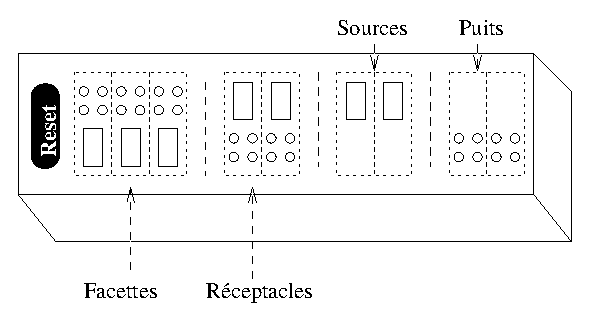
\includegraphics{figures/component-tester.eps}    
     \caption{Testeur de composant}
     \label{fig-tester-composant}
 \end{figure}

 L'\textsf{IUT} est donc  vu comme une
 bo\^{\i}te noire dont le seul comportement observable est donn\'e par
 les diff\'erents \'ecrans accessibles. Ce sc\'enario de test ne
 d\'efinit bien \'evidemment pas le comportement du testeur, c'est
 \`a dire la mani\`ere dont celui-ci agit en poussant les boutons en
 fonction des informations produites par le sc\'enario de  test. 

Le comportement du testeur est bien \'evidemment d\'etermin\'e par
la sp\'ecification que l'on souhaite v\'erifier, autrement dit par
un ensemble d'automates \textsf{FIDL} synchronis\'es. Parmi tous ces
automates nous distinguerons les cat\'egories suivantes :  
\begin{itemize}
  \item les automates dits \emph{actifs} sont moteurs dans le
  processus de test. C'est en fonction d'eux qu'est calcul\'ee la
  fonction d'\'evaluation ;
\item les automates \emph{passifs} ne jouent aucun r\^ole dans le
  processus de d\'ecision, ils peuvent \^etre amen\'e \`a
  r\'eagir  aux sollicitations de l'\textsf{IUT} ou produire des
  messages permettant au processus de test de progresser en fonctions
  des contraintes de synchronisation.
\end{itemize}

De plus, nous distinguerons les automates dits bien form\'es  dont le
comportement est une alternance d'entr\'ees et de sorties des
automates quelconques dont les entr\'ees/sorties peuvent \^etre
arbitrairement entrelac\'ees. Les premiers correspondent \`a la
sp\'ecification du comportement d'une interface et les seconds \`a
une partie du comportement d'un composant.

\subsection{Algorithme g\'en\'eral}

Pour prendre en compte l'existence de plusieurs ports de communication
et de plusieurs automates synchronis\'es repr\'esentant la
sp\'ecification, il est n\'ecessaire de modifier substantiellement l'algorithme de
base de la figure \ref{fig-algo-test-base}. Cet algorithme est
fondamentalement s\'equentiel alors qu'un composant est
potentiellement constitu\'e de flots d'ex\'ecution parall\`eles,
m\^eme si le degr\'e de parallelisme est restreint par les
synchronisations entre ports.

Le principe de fonctionnement de cet algorithme est le suivant :
\begin{itemize}
  \item parmi l'ensemble des automates synchronis\'es, un est
    distingu\'e comme \'etant l'automate actif $A$ ;
  \item comme pr\'ec\'edemment, une fonction \textsf{select} de
    s\'election de la prochaine action \`a effectuer est
    appel\'ee mais cette fois uniquement en fonction de l'automate
    actif $A$. Cette fonction retourne soit le symbole
    \textsf{terminate},
    soit le symbole \textsf{reset}, soit un ensemble ordonn\'e
    \textsf{acts} de lettres de $\Sigma_A$ ;
  \item pour chacune de ces lettres, on essaye de construire une
    s\'equence de synchronisation dans l'ensemble des automates
    $S$ : 
    \begin{itemize}
      \item si aucune s\'equence de synchronisation ne peut \^etre
        construite apr\`es \'epuisement de \textsf{acts}, alors la
        s\'equence de test courante indique une \emph{erreur dans la
          sp\'ecification} et le processus de test est arr\^et\'e,
      \item sinon, on r\'ealise les actions de
        la s\'equence $\sigma$ jusqu'\`a atteindre l'\'el\'ement de
        \textsf{acts} synchronis\'e ou jusqu'\`a ce qu'un d\'ecalage
        (conforme) soit constat\'e sur un message de sortie, et on
        recommence la proc\'edure. La figure \ref{fig-algo-execute}
        d\'etaille l'ex\'ecution de la s\'equence de synchronisation.
    \end{itemize}
\end{itemize}


\begin{figure}[htbp]
    \centering
 \begin{lstlisting}[linewidth=\textwidth,mathescape=true,numbers=left,numberstyle=\tiny,literate={:=}{{$\leftarrow$}}1 ]
 Input : $S=\{A_i = (Q_i,q_0^i,\Sigma_i,\delta_i), 1\leq i \leq n\}$
         $A \in S$  // un automate actif dans la sp\'ecification
         $I$ une implantation sous test          
 Output : failures     
 T := $\emptyset$
 Trace := $\epsilon$ 
 State := $(q_0^1,\dots, q_0^n)$ 
 Failures := $\emptyset$
 outerloop:
  while true 
    action := select(A,State,T,Trace)
    switch action
       case terminate: 
           return Failures
       case reset:
           T := T $\cup \{\mathsf{Trace}\}$
           State := $(q_0^1,\dots, q_0^n)$
           Trace := $\epsilon$
       case $acts \subset \Sigma_A$ :
            for each act $\in acts$ 
               word := $\epsilon$
               letter := $a$
               explore(State) 
               if word != $\epsilon$ then
                  execute(word)
                  continue outerloop 
               end
            end
            // problem
            return Failures
      end  
   end 
 \end{lstlisting}
 \caption{Algorithme de test de composants \textsf{FIDL}}
 \label{fig-algo-test-fidl}
 \end{figure}

Cet algorithme utilise une proc\'edure de recherche \textsf{explore} d'un mot
permettant de synchroniser plusieurs automates et se terminant par une
lettre particuli\`ere. Le principal int\'er\^et de l'agorithme est
qu'il \'evite de calculer un porduit de synchronisation global et
donc une sp\'ecification globale du composant test\'e.

\begin{figure}[htbp]
    \centering
 \begin{lstlisting}[linewidth=\textwidth,mathescape=true,numbers=left,numberstyle=\tiny,literate={:=}{{$\leftarrow$}}1 ]
function execute(word,S,I,State,Trace)
                  for $i \in \{1,\dots,\# word\}$ 
                     if word[i] $\in Out(\Sigma_S)$        
                        out := output(I) 
                        if out != $\theta$ then
                           Trace := Trace.out
                            //  unexpected output 
                            if $out \not\in \delta(State)$ then 
                               Failures := Failures $\cup$ Trace
                               T := T $\cup \{\mathsf{Trace}\}$
                               State := $q_0$
                               Trace := $\epsilon$
                            else if out $\neq$ word[i]
                               State := fire(out)
                               continue outerloop  // recommence la
                                                   // proc\'edure de d\'ecision
                             end
                        else 
                           //  a deadlock  
                           Trace := Trace.$\theta$
                           Failures := Failures $\cup$ Trace
                           T := T $\cup \{\mathsf{Trace}\}$
                           State := $q_0$
                           Trace := $\epsilon$
                        end
                     else if ! input(I,word[i]) 
                        //  refused input 
                        Trace := Trace.$\theta$
                        Failures := Failures $\cup$ Trace
                        T := T $\cup \{\mathsf{Trace}\}$
                        State := $q_0$
                        Trace := $\epsilon$
                     else
                        Trace := Trace.word[i]
                        State := fire(S,action)
                     end
                  end
                  // continue
 \end{lstlisting}
 \caption{Ex\'ecution d'une s\'equence de synchronisation}
 \label{fig-algo-execute}
 \end{figure}

Cette restriction est bien \'evidemment incorrecte dans le cas
g\'en\'eral o\`u les contraintes sont des fonctions arbitraires
puisque la r\'esolution d'un ensemble de contraintes peut d\'ependre
d'un certain nombre de \emph{tour de boucles} dans l'automate, par
exemple lorsque la contrainte d\'epend de calculs fait sur la trace.

On va donc choisir l'approche moins puissante mais dans la majorit\'e
des cas plus efficace consistant \`a s\'electionner un mot candidat
\`a l'aide de l'algorithme donn\'e puis \`a r\'esoudre les
contraintes restantes pour instancier les variables.

On notera que dans le cas d'automates \textsf{FIDL}, et de mani\`ere
plus g\'en\'eral dans le cas d'\textsf{IOLTS}, la d\'ecouverte d'un
mot permettant de synchroniser diff\'erents automates sur un objectif
commun n'est aucunement une garantie que l'action correspondant \`a
la lettre recherch\'ee soit effectivement r\'ealis\'ee dans le cas
o\`u certains des automates consid\'er\'es sont ind\'etermin\'e
en sortie pour des \'etats atteints par le mot de synchronisation. 
 
\subsubsection{Conformit\'e des ports synchrones}

La premi\`ere phase de la v\'erification de la conformit\'e d'un
composant consiste donc \`a tester celui-ci par rapport \`a la
sp\'ecification de chacun de ses ports. Dans ce cas de figure,
l'automate correspondant au port verifi\'e est consid\'er\'e comme
actif et tous les autres automates impliqu\'es dans la sp\'ecification
du composant sont passifs. 

\subsubsection{Conformit\'e du composant}

Dans une deuxi\`eme phase, la conformit\`e de l'\textsf{IUT} au
comportement sp\'ecifi\'e par le composant est v\'erifi\'ee pour
chacun des automates synchronis\'es de la sp\'ecification du
composant. Chacun alternativement est donc l'automate actif au cours
d'une session de test et tous les autres automates sont passifs. 

\section{Conclusion}

L'approche que nous proposons se distingue des travaux existant sur le
test d'\textsf{IOLTS} par l'absence de sp\'ecification globale est la
volont\'e de ne pas construire celle-ci. Cette approche se situe
ainsi \`a mi-chemin des strat\'egies de test bas\'ees sur la
d\'efinition d'un objectif de test ad-hoc par le concepteur et des
strat\'egies de test syst\'ematiques bas\'ees sur la satisfaction
d'un crit\`ere de couverture. De la premi\`ere, nous conservons la
taille relativement faible des suites de test et des testeurs en ne
testant \`a chaque \'etape qu'une partie de la
sp\'ecification. Mais l'utilisation d'une strat\'egie
d'\'evaluation des cas de test par une fontion arbitraire
d\'efinissant un certain degr\'e de couverture permet de conserver
au test unitaire de composants son caract\`ere syst\'ematique. 

Bien entendu, en l'absence de couverture compl\`ete du comportement
du composant, on ne peut tirer du r\'esultat d'une telle proc\'edure
de test que des conclusions dont la valeur d\'epend de la confiance
mise dans les crit\`eres d'\'evaluation choisis par le testeur.

%% Nous allons dans ce chapitre d\'efinir une strat\'egie
%% de s\'election des ex\'ecutions de tests applicable \`a l\'{}ensemble des
%% objectifs de test d\'efinis pr\'ec\'edemment. Cette strat\'egie
%% doit nous permettre d'atteindre deux buts contradictoires :
%% \begin{itemize}
%%   \item minimiser l'effort de test ;
%%   \item maximiser la fiabilit\'e du r\'esultat obtenu.
%% \end{itemize}
%% Pour ce faire, nous allons d\'efinir diff\'erentes mesures \`a
%% partir d\'{}une sp\'ecification sous forme d'automate \textsf{FIDL} :
%% une \emph{distance} entre les diff\'erentes ex\'ecutions possibles de
%% l'automate, et une \emph{complexit\'e} de diff\'erentes parties de
%% la sp\'ecification. Ces deux mesures seront int\'egr\'ees pour
%% construire une fonction d'\'evaluation, elle-m\^eme utilis\'ee
%% comme heuristique dans un algorithme de recherche de type
%% \textsc{Minimax}. La combinaison de ces deux mesures doit nous
%% permettre d'assurer d'une part un certain  degr\'e de
%% \emph{couverture} de la sp\'ecification, et d'autre part d'optimiser
%% l'effort de test en faisant porter celui-ci sur les parties de la
%% sp\'ecification les plus pathog\`enes. 

%% \section{Distance}
%% \label{sec:distance--limite}

%% Nous avons vu dans le chapitre \ref{chap-etatarttest} le r\^ole que
%% jouent les notions de \emph{couverture} et de \emph{crit\`ere} dans
%% le test dit structurel. Nous avons remarqu\'e par ailleurs que ces
%% notions devenaient pertinentes dans le test fonctionnel du fait de la
%% complexit\'e croissante des sp\'ecifications. \`A partir d'une certaine taille,
%% il devient infaisable d'appliquer des algorithmes exhaustifs pour
%% \'etablir la conformit\'e d'une application avec sa
%% sp\'ecification. Un certain nombre de travaux proposent des
%% crit\`eres, inspir\'es du test structurel, pour \'etablir la
%% conformit\'e avec un mod\`ele, qu'il soit sous forme d'\textsf{EFSM}
%% ou de \textsf{(IO)LTS}.

%% Nous nous basons sur ces travaux pour proposer une mesure de la
%% \emph{distance} entre mots d'un langage et donc de la
%% \emph{couverture} d'un langage par un ensemble de mots qui soit
%% effectivement calculable, intuitivement simple et pertinente et qui
%% constituera un outil efficace de s\'election des cas de tests dans un
%% algorithme de test \emph{online}. Cette distance est bas\'ee sur le
%% principe du calcul de la fonction de \emph{Parikh} que nous introduirons tout d'abord. Nous d\'efinissons
%% ensuite une mesure de la couverture entre mots et montrons que cette
%% mesure est pertinente et permet d'approcher d'aussi pr\`es que l'on
%% veut un langage --- rationnel --- quelconque. Nous terminons cette
%% section par le d\'etail des algorithmes nous permettant de manipuler
%% cette notion dans le cadre du test. 

%% \subsection{Graphes \& Matrices}

%% La matrice associ\'ee \`a un graphe $G$ dite aussi \emph{matrice
%% d'adjacence} est la matrice carr\'ee $M\in \mathbb{B}^{S \times{}S}$ telle
%% que $\forall s_i,s_j \in S$, 
%% $$
%% M_{s_i,s_j}=
%% \left\{\begin{array}{ll}
%% 1,&\mbox{~si~} \exists e \in E,\iota(e) = s_i,
%% \omega(e)=s_j \\
%% 0,&\mbox{~sinon~}.
%% \end{array}\right.
%% $$

%% La \emph{matrice d'incidence} d'un graphe $G=(S,E)$ est la matrice $I$
%% de dimension $n\times{}m$ o\`u $m=\vert E \vert$, telle que :
%% $$
%% I_{s_i,e_j} = \left\{
%%     \begin{array}{ll}
%%         -1,\mbox{~si~} \iota(e_j) = s_i \\
%%         +1, \mbox{~si~} \omega(e_j) = s_i \\
%%         0, \mbox{~sinon~}. 
%%     \end{array}\right.
%% $$

%% %% Soit $X\subset S$ un ensemble de sommets, $\omega^+(X)$ est l'ensemble
%% %% des arcs incidents ext\'erieurs  \`a $X$ 
%% %% $$
%% %% \omega^+(X) = \{a\in A\mid \iota(a)\in X, \tau(a)\not\in X\}.
%% %% $$ 
%% %% De m\^eme, $\omega^-(X)$ est l'ensemble des arcs incidents
%% %% int\'erieurs \`a $X$ :
%% %% $$
%% %% \omega^-(X) = \{a\in A\mid \iota(a)\not\in X, \tau(a)\in X\}.
%% %% $$ 
%% %% $\omega(X)= \omega^+(X) \cup \omega^-(X)$ est l'ensemble des arcs
%% %% incidents \`a $X$. 

%% %% Un \emph{cocycle} est un ensemble d'arcs incidents \`a $X$
%% %% $\omega(X)$. Un cocycle est \'el\'ementaire s'il est constitu\'e de
%% %% l'ensemble des arcs reliant entre eux deux sous-graphes connexes de
%% %% $G$. 

%% Soit $f:E\rightarrow \mathbb{Z}$ (ou dans $\mathbb{H}$ un
%% groupe quelconque) une application. Pour  chaque \'el\'ement $s$ de $S$, on
%% d\'efinit la valeur de $f$ en $s$ : 
%% $$
%% f[s] \stackrel{\mathrm{def}}{=} \sum_{(s,s')\in E} f((s,s')) -
%% \sum_{(s',s)\in E} f((s',s))
%% $$
%% L'application $f$ est un \emph{flot} si 
%% $$
%% \forall s\in S, f[s] = 0.
%% $$
%% Cette propri\'et\'e de conservation des flux entrants et sortants
%% est appel\'ee loi de \emph{Kirchoff}. 

%% Un $(s,t)$-flot pour tout couple de sommets $s$ et $t$ est une
%% application $f:E\rightarrow \mathbb{Z}$, not\'e $(f,s,t)$ telle que : 
%% $$
%% \forall q\in S, f[q] = \left\{
%%     \begin{array}{ll}
%% -1, \mbox{~si~} q=s, \\
%% +1, \mbox{~si~} q=t, \\
%% 0, \mbox{~sinon.} \\
%%     \end{array}\right.
%% $$

%% Un flot $(f,s,t)$ sera dit \emph{connect\'e} si le sous
%% graphe de $G$ induit par l'ensemble des arcs $E'=\{e\in E\mid f(e)\neq
%% 0\}$ est connexe. Un $(s,t)$-flot $(f,s,t)$ peut \^etre
%% ttransform\'e en un flot $f$ en ajoutant un arc $(t,s)$ tel que
%% $f((t,s) = 1$.

%% \subsection{Fonction \& Vecteur de Parikh}

%% Soit $\Sigma$ un alphabet fini totalement ordonn\'e de taille $k$, l'\emph{application de Parikh}\cite{parikh-cf} est un morphisme
%% $\Psi:\Sigma^* \rightarrow \mathbb{N}^k$, avec 
%% \begin{align*}
%% \forall a_i\in \Sigma, \Psi(a_i) = \left(
%%     \begin{array}{c}
%% x_1\\ x_2 \\ \vdots \\ x_k
%% \end{array}
%% \right) \mbox{~avec~} x_i=1, x_j=0
%% \mbox{~pour~} j\neq i,
%% &\mbox{~et~}&
%% \begin{array}{rl}
%% \Psi(\epsilon) &=\vec{0} \\\
%% \Psi(u.a) &= \Psi(u)+\Psi(a).\\
%% \end{array}
%% \end{align*}

%% Pour tout $u$, $\Psi(u)$ est appel\'e \emph{vecteur de
%%   Parikh}. Par extension, on notera $\Psi(L)=\{\Psi(u), u \in L\}$ l'image d'un langage
%%   $L$.  

%% \subsubsection{Ensembles lin\'eaires \& semilin\'eaires}

%% Un ensemble $L\in \mathbb{N}^p$ est lin\'eaire ssi il existe une \emph{base} 
%% $\vec{b}\in \mathbb{N}^p$ et un ensemble fini de \emph{phases} 
%% $P=\{\vec{p}_1,\dots,\vec{p}_1\} \subseteq \mathbb{N}^p$ tels que
%% $L=\{\vec{x} \mid \vec{x} = \vec{b} + \sum_{i=1}^k \lambda_i
%% \vec{p}_i, \lambda_i\in \mathbb{N}\}$. Un ensemble \emph{semilin\'eaire} est
%% une union finie d'ensembles lin\'eaires. On notera un ensemble lin\'eaire $(c,P)$ o\`u $c$ est
%% une constante --- la base --- et $P$ un ensemble \'eventuellement
%% vide de \emph{phases}, et un ensemble semilin\'eaire $\cup_{i=1}^n
%% (c_i,P_i)$. 

%% D'apr\`es le th\'eor\`eme de Parikh, pour tout langage
%% alg\'ebrique et donc pour tout langage
%% rationnel, l'ensemble des vecteurs de
%% Parikh de ce langage, c'est \`a dire l'ensemble 
%% $\Psi(L)$ est semilin\'eaire. On peut voir l'ensemble $\Psi(L)$
%% comme une repr\'esentation sous forme alg\'ebrique de l'ensemble des
%% cycles --- les phases --- possibles dans le langage $L$. Toute solution de l'un ou l'autre des
%% syst\`emes d'\'equations de l'ensemble semilin\'eaire est l'image
%% de Parikh d'un ou plusieurs mots du langage $L$. 

%% Pour obtenir l'application de Parikh pour un langage donn\'e, il est
%% donc n\'ecessaire  de construire les langages lin\'eaires d\'efinissant
%% $\Psi(L)$. 
%% Cette construction peut se faire  \`a partir de l'expression
%% rationnelle du langage\cite{litow-semilinear,lugiez-semilinear}. Si $E$ est une expression rationnelle sur un alphabet
%% totalement ordonn\'e $\Sigma$ de taille $k$ et $\Psi:\Sigma^* \rightarrow \N^k$ la
%% fonction de Parikh associ\'ee, on construit inductivement un
%% semilin\'eaire, c'est \`a dire un ensemble fini d'\'equations lin\'eaires \`a coefficients dans $\N^k$
%% permettant de calculer l'image de Parikh du langage $L(E)$ de la
%% mani\`ere suivante. Soit 
%% \begin{align*}
%%     \Psi(E) = \bigcup_{i=1}^n (c_{i},P_i) &\mbox{~et~}& \Psi(F) = \bigcup_{j=1}^m (c_{j},P_j),
%% \end{align*}
%% alors :
%% \begin{align*}
%%     \Psi(E+F) &= \Psi(E) \cup \Psi(F) \\
%%     \Psi(E^*) &= \bigcup_{i=1}^n (0,P_i\cup \{c_{i,0}\}) \\
%%     \Psi(E.F) &= \bigcup_{i=1}^n \bigcup_{j=1}^m (c_{i}+c_{j},P_i \cup P_j)\\
%%     \Psi(a) &= (\vec{a}_i,\emptyset).
%% \end{align*}
%% On remarque que cette construction est simple mais co\^uteuse puisque la
%% concat\'enation provoque une croissance exponentielle du nombre
%% d'\'equations. Elle permet toutefois d'\'eviter la construction
%% explicite de l'automate \'equivalent \`a une expression rationnelle
%% $E$ qui est aussi une op\'eration co\^uteuse.

%% \subsubsection{Image de Parikh \& Graphes}

%% \cite{seidl-icalp04} s'int\'eresse \`a la construction, \`a partir
%% d'un automate non-d\'eterministe $A=(Q,q_0,T,\Sigma,\delta)$, d'une formule
%% de l'arithm\'etique de \emph{Presburger} quantifi\'ee
%% existentiellement dont les mod\`eles sont les
%% vecteurs de Parikh du langage reconnu par l'automate. Rappelons que 
%% les ensembles
%% semilin\'eaires sont les mod\`eles des formules de l'arithm\'etique
%% de Presburger, c'est \`a dire de l'arithm\'etique sur l'ensemble
%% $\N$ utilisant uniquement l'op\'erateur $+$ et la comparaison
%% $\leq$. 

%% L'algorithme propos\'e se base sur la d\'efinition d'un \emph{flot}
%% dans le graphe sous-jacent \`a un automate ce qui permet d'obtenir le
%% r\'esultat suivant :

%% \begin{prop}[\cite{seidl-icalp04}, app. A.1]
%% \label{thr:seidl}
%% Soit $L_A$ le langage reconnu par un automate $A$ sur un alphabet
%% $\Sigma$ totalement ordonn\'e de taille $k$. Un vecteur $\vec{u} \in
%% \N^k$  est dans l'image de Parikh de $L_A$, ssi
%% il existe un \emph{$(q_0,t)$-flot connect\'e} $(f,q_0,t)$, pour
%% $q_0$ l'\'etat initial de $A$ et $t\in T$ un \'etat terminal, et
%% $f:\delta\rightarrow \N$ une application tels que :
%% $$
%% \forall a\in \Sigma, \vec{u}[a] = \sum_{q \in \delta(p,a)} f(p,a,q).
%% $$ 
%% \end{prop} 

%% \subsection{Applications aux automates}

%% Nous nous basons sur les d\'efinitions et r\'esultats
%% pr\'ec\'edents concernent les vecteurs de Parikh pour d\'efinir une
%% notion diff\'erente mais connexe : l'ensemble des vecteurs
%% repr\'esentant les diff\'erentes \emph{transitions} de l'automate
%% qu'il est possible de franchir en reconnaissant un mot. Nous
%% appelerons les \'el\'ements de cet ensemble des \emph{P-vecteurs} et
%% l'ensemble lui-m\^eme un \emph{P-ensemble}.  On
%% constatera que la construction d'un P-ensemble pour un langage est similaire \`a la
%% construction de l'ensemble des images de Parikh d'un langage, \`a un
%% re\'etiquetage pr\`es des lettres du langage pour distinguer les
%% diff\'erentes occurences de lettres sur diff\'erentes transitions. 

%% L'objectif de cette section est de caract\'eriser : 
%% \begin{itemize}
%%   \item l'ensemble des P-vecteurs qui sont l'image des mots
%%     reconnus par un automate ;
%%   \item l'ensemble des mots qui ont pour P-vecteur un certain
%%   vecteur $\vec{v}$.
%% \end{itemize}

%% Soit un automate fini
%% d\'eterministe $A=(Q,q_0,T,\Sigma,\delta)$ et son langage
%% $L_A$. Soit $G=(Q,E)$ le
%% graphe de l'automate $A$, \`a chaque arc $(q,q')\in E$ est
%% associ\'e un indice entre $1$ et $m = \mid E\mid$ de sorte que $E$ soit
%% totalement ordonn\'e. Nous utiliserons indiff\'eremment des
%% \'el\'ements de $E$ ou des entiers en tant qu'indices. 

%% Nous d\'efinissons $\psi$, la fonction permettant de construire le
%% P-ensemble pour le langage d'un automate $A$. $\psi:E \rightarrow
%% \N^{m+1}$, est d\'efinie comme :
%% $$
%% \psi(e_i) = \left(
%%     \begin{array}{c}
%% 0 \\x_1\\ x_2 \\ \vdots \\ x_{m}
%% \end{array}
%% \right) \mbox{~avec~} x_i=1 \mbox{~et~} x_j=0
%% \mbox{~pour~} j\neq i. 
%% $$
%% On notera $\mathbf{1}$ le vecteur $(1,0,\dots,0) \in  \N^{m+1}$ et
%% $\mathbf{0}$ le vecteur $(0,0,\dots,0)$. Le lecteur attentif aura
%% remarqu\'e que le vecteur est de taille $m+1$. L'utilit\'e de cette
%% dimension suppl\'ementaire appara\^{\i}tra plus clairement dans la
%% section consacr\'ee \`a la distance.

%% L'application $\psi$ est \'etendue aux  mots $u \in Pref(L_A)$,
%% repr\'esent\'es par un chemin $e_1e_2 \dots e_k$ de longueur $k$ dans l'automate
%% $\cal A$ de la mani\`ere suivante :
%% $$
%% \psi(e_1e_2\dots e_k) = \sum_{j=1}^k\psi(e_j) + \left\{
%%     \begin{array}{ll}
%% \mathbf{1}, \mbox{~si~} \omega(e_k) \in T, \\
%% \mathbf{0}, \mbox{~sinon~}. \\
%%     \end{array}\right.
%% $$
%% Tout mot $u$ de $L_A$ est donc repr\'esent\'e comme un vecteur de $m+1$
%% \'el\'ements \`a coefficients entiers repr\'esentant le nombre
%% d'occurences de chaque transition franchie pour reconna\^{\i}tre $u$
%% dans $A$.  Bien \'evidemment, l'application $\psi$ n'est pas
%% g\'en\'eralement injective : \`a plusieurs mots peuvent 
%% correspondre un m\^eme vecteur. 

%% \subsubsection{Repr\'esentation matricielle de $\psi(L_A)$}

%% On va caract\'eriser $\psi(L_A)$, le P-ensemble associ\'e \`a $A$ pour faire
%% correspondre \`a chaque vecteur $\vec{v}=(1,v_1,\dots,v_m)\in \N^{m+1}$ l'ensemble des
%% mots $v$ de $L_A$ tels que $\psi(v) = \vec{v}$. Ce vecteur correspond
%% \`a un mot $v$ si et seulement si il existe un chemin $\sigma$ dans
%% l'automate $A$ de $q_0$ vers $q$ avec $\vert \sigma \vert =
%% \sum_{i=1}^m v_i - 1$. Le th\'eor\`eme \ref{thr:seidl}
%% caract\'erise $\Psi(L_A)$  par les
%% propri\'et\'es d'un flot entre $q_0$ et un \'etat terminal de
%% $A$. Nous nous basons sur cette d\'efinition pour d\'ecrire
%% $\psi(L_A)$ comme l'ensemble des solutions d'un syst\`eme lin\'eaire
%% d'\'equations poss\'edant une certaine structure. 

%% On va se servir de la
%% \emph{matrice d'incidence} du graphe de l'automate $\cal A$ \'etendue
%% \`a $m+1$. Cette extension est not\'ee $\mathfrak{M}$ et d\'efinie
%% comme :
%% $$
%% \mathfrak{M} = 
%% \left(\begin{array}{cc}
%%         1 & 0 \\
%%         0 & \fbox{I} 
%%     \end{array}\right).
%% $$ 

%% Un vecteur $\vec{v} \in \N^{m+1}$ est un P-vecteur s'il est
%% solution d'une \'equation : 
%% \begin{equation}
%% \mathfrak{M}. \vec{X}  = S_t,\label{eq:sys-parikh}
%% \end{equation}
%% o\`u $X$ est un vecteur colonne de $m+1$ \emph{variables} distinctes
%% et $S^t$ est une famille de vecteurs indic\'ee par les \'el\'ements
%% de $T$, l'ensemble des \'etats terminaux de l'automate $A$ 
%%  de taille $\N^{1+Q}$  tel que :
%% \begin{align*}
%% S_1^t = 1 \quad&\mbox{et}&\quad   S_{q_i} = \left\{
%%     \begin{array}{ll}
%% -1,&\mbox{~si~} q_i=q_0 \\
%% +1,&\mbox{~si~} q_i=t\\
%% 0,&\mbox{~sinon~}.
%%     \end{array}\right.
%% \end{align*}

%% Autrement dit, on a un syst\`eme lin\'eaire de $n$ \'equations et
%%  $m$ variables \`a r\'esoudre pour trouver le ou
%% les mots  $v$ correspondant au vecteur $\vec{v}$. 
%% Ce syst\`eme exprime le fait que :
%% \begin{itemize}
%%   \item tout vecteur est un \emph{flot} et par cons\'equent la somme
%%     des poids des arcs entrant et sortant doit \^etre 0 sauf pour
%%     l'\'etat de d\'epart et l'\'etat d'arriv\'ee du flot. Cette
%%     condition s'exprime facilement comme un syst\`eme d'\'equations
%%     lin\'eaires induit par la matrice d'incidence $I$ ;
%%   \item pour l'\'etat de d\'epart et celui d'arriv\'ee, la valeur total des poids
%%     associ\'es aux arcs entrants  et sortants est respectivement de
%%     $-1$ et $1$. 
%% \end{itemize}
%% Comme il peut exister plusieurs \'etats terminaux, plusieurs
%% solutions sont possibles et il est donc n\'ecessaire de distinguer
%% les diff\'erentes possibilit\'es d'attieindre un \'etat terminal. 

%% Dans le cas o\`u l'automate $A$ a un seul \'etat terminal $t$, alors
%% la matrice $\mathfrak{M}$ peut \^etre red\'efinie comme 
%% $$
%% \mathfrak{M} = 
%% \left(\begin{array}{cc}
%%         1 & 0 \\
%%  \fbox{$S_t$} & \fbox{$I$}  \\
%%     \end{array}\right)
%% $$ 
%% et l'\'equation \eqref{eq:sys-parikh} se r\'e\'ecrit plus
%% simplement comme 
%% \begin{equation}
%%     \label{eq:sys-parikh-normal}
%% \mathfrak{M}. \vec{X} = \mathbf{0}.
%% \end{equation}

%% Cette condition est n\'ecessaire mais n'est pas suffisante car elle
%% n'exprime pas l'exigence de connexit\'e entre tous les \'etats
%% participant du flot. On peut exprimer le fait qu'un P-vecteur
%% repr\'esente un chemin connexe en le comparant aux plus petits
%% chemins permettant d'atteindre chacune des transitions parcourues par
%% le P-vecteur. 

%% Pour tout arc $e_i=(q',q)$, soit
%% $c(e_i)$ l'ensemble des P-vecteurs des $(q_0,q)$-chemins $\mu{}$ tels que
%%  $\vert \mu{}\vert = k$ et $E(\mu{})[k-1]=e_i$:
%% $$
%% c(e_i) = \{\psi(u) \mid u=va, q_0 \xrightarrow{v} q'
%% \xrightarrow[e_i]{a}, \mbox{~et $v$ est minimal~}\}.
%% $$
%% Alors, tout P-vecteur $\vec{v}=(1,v_1,\dots,v_m)$ solution de l'\'equation
%% \eqref{eq:sys-parikh} doit de plus v\'erifier la condition suivante :
%% \begin{equation}
%%     \label{eq:parikh-connect}
%%     \forall v_i \neq 0, \exists \vec{c}\in c_i, \vec{c}\leq \vec{v},
%% \end{equation}
%% o\`u $\vec{w}\leq \vec{v}$ si et seulement si $\forall i,1\leq i\leq m, w_i\leq v_i$.

%% \paragraph{Exemple}

%% Par exemple, soit l'automate pr\'esent\'e dans la figure
%% \ref{fig-sample-dfa-distance} o\`u les transitions sont indic\'ees
%% de la mani\`ere suivante :
%% $$
%% \begin{array}{rcl}
%% (2 , b , 0)&\mapsto &1\\
%%  (3 , b , 0)&\mapsto &2\\
%% (1 , a , 3)&\mapsto &3\\
%%  (3 , c , 0)&\mapsto &4\\
%%  (0 , a , 2)&\mapsto &5,
%% \end{array}
%% $$
%% le vecteur associ\'e au mot $abab$ est $(1,1,1,1,0,1)$, celui
%% associ\'e au mot $acabab$ est $(1,2,0,1,1,2)$. Le vecteur associ\'e
%% \`a $\epsilon$ est d\'efini comme $(1,0,0,0,0,0)$.

%% La matrice $\mathfrak{M}$ est 
%% $$
%% \left(\begin{array}{cccccc}
%% 1 & 0 &  0 &  0 & 0  & 0  \\
%% 0 & 1 &  1 &  0 & 1  & -1 \\
%% 0 & 0 &  0 & -1 & 0  & 0  \\
%% 0 & -1 & 0 &  0 & 0  & 1  \\
%% 0 & 0 & -1 &  1 & -1 & 0  \\
%% \end{array}\right), 
%% $$
%% et par cons\'equent l'ensemble des vecteurs de Parikh est donn\'e
%% par les solutions au syst\`eme d'\'equations suivants :
%% $$
%% \left\{\begin{array}{ccccccr}
%% x_1 &+ x_2 &&+ x_4 &- x_5  &=& 1 \\
%% &&- x_3 && &=& -1 \\
%% -x_1 &&&+ x_4 &&=& 0 \\
%% &-x_2 &+ x_3 &-x_4 &&=& 0 \\
%% \end{array}\right..
%% $$

%% \begin{figure}
%%     \centering
%% 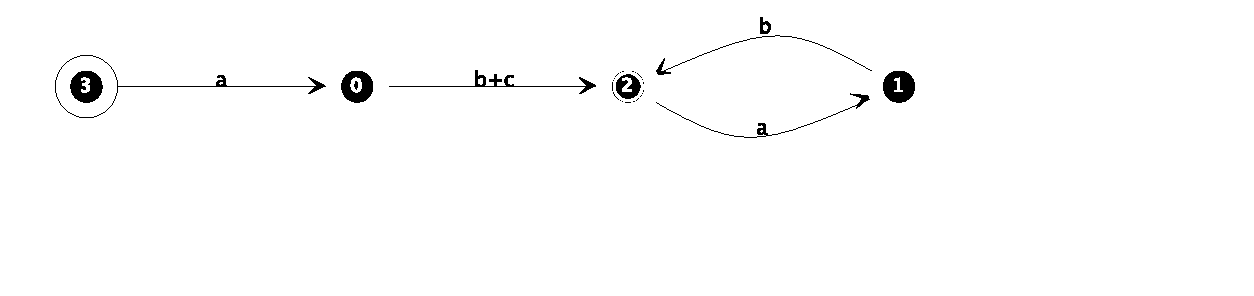
\epsfig{width=.5\textwidth,file=figures/fig-sample-dfa-distance.eps}    
%%     \caption{Automate d\'eterministe minimal pour le langage $a(b+c)(ab)^*$}
%%     \label{fig-sample-dfa-distance}
%% \end{figure}

%% \subsubsection{Calcul de $\psi^{-1}(\vec{v})$}

%% \'Etant donn\'e un vecteur de Parikh $v$ appartenant \`a l'image de
%% $L_A$, on souhaite pouvoir reconstituer le ou les mots dont $v$ est
%% l'image. Ce probl\`eme a deux formes distinctes :
%% \begin{enumerate}
%%   \item reconstuire un mot $u$ appartenant \`a $\psi^{-1}(v)$ ;
%%   \item reconstruire $\psi^{-1}(v)$.
%% \end{enumerate}

%% Le premier probl\`eme est  simple : on parcours l'automate en mettant \`a jour le vecteur en fonction des
%% transitions franchies jusqu'\`a atteindre le vecteur $\mathbf{1}$ qui
%% doit correspondre \`a l'atteinte d'un \'etat terminal. L'algorithme
%% est pr\'esent\'e dans la figure \ref{fig-algo-inverseimage} : il
%% retourne le mot construit s'il existe, c'est \`a dire si $v\in
%% \psi(L_A)$ et $\epsilon$ sinon. 

%% \begin{figure}[htbp]
%%     \centering
%%     \begin{lstlisting}[mathescape=true,literate={:=}{{$\leftarrow$}}1 ]
%% Input: $A=(Q,q_0,T,\Sigma,\delta)$ un automate 
%%        $v\in \N^{\vert \delta\vert+1}$ un vecteur  de Parikh
%% Output: un mot $u \in L_A$, si $v\in \psi(L_A)$

%% $q$ := $q_0$
%% $u$ := $\epsilon$
%% $C$ := base de cycle de $A$

%% while $v \neq \mathbf{1}$
%%    out := out(v,q)
%%    if $\vert out \vert$ > 1 then
%%        c := $\{ e \mid (n,e) \in out,e\in C\}$
%%        // verifie la correction de v
%%        c' := $\{ e \mid (n,e) \in out,e\not\in C\}$
%%        if $\vert c' \vert > 1$ then
%%           return $\epsilon$
%%        end
%%        // choisit un cycle s'il y en a un
%%        if $\vert c \vert > 0$ then 
%%           t := $e=(q,a,q') \in c$
%%        else 
%%           t := $e=(q,a,q') \in c'$
%%        end
%%        // franchit la transition
%%        u := $u.a$
%%        q := $q'$
%%        v := $v - \psi(e)$
%%    else
%%       return $\epsilon$
%%    end
%% end
%% return $u$

%% // fonction auxiliaire
%% out(v, q) $\stackrel{}{=}[\mathrm{def}] \{ (v_i,e_i) \mid v_i>0, e_i =
%% (q,q') \in E\}$

%%  \end{lstlisting}    
%%      \caption{Calcul d'un mot de $\psi^{-1}(v)$}
%%      \label{fig-algo-inverseimage}
%%  \end{figure}

%% Le second probl\`eme est  plus complexe et plus int\'eressant car il n\'ecessite de
%% calculer une op\'eration de cl\^oture commutative pour tous les
%% cycles apparaissant dans le vecteur $v$ entre deux cocycles. Dans
%% l'imm\'ediat, nous ne nous attarderons pas sur ce calcul qui
%% n\'ecessiterait des d\'eveloppements importants.

%% %% Cette repr\'esentation pr\'esente l'inconv\'enient d'\^etre assez
%% %% \og gourmande\fg alors m\^eme que certains \'el\'ements du vecteurs
%% %% sont li\'es les uns aux autres. On la raffine donc en utilisant comme
%% %% \'el\'ements du vecteurs les \emph{bases de cycle} du graphe
%% %% sous-jacent \`a l'automate $A$. Les bases de cycle d'un graphe
%% %% dirig\'e sont les chemins du graphe tels que tout autre chemin peut
%% %% s'exprimer comme une combinaison lin\'eaire d'\'el\'ements de la
%% %% base. Plus formellement :

%% %% \begin{definition}[Base de cycle d'un graphe $G$]
%% %% Pour tout graphe dirig\'e $G=(S,E)$, une base de cycle est un
%% %% ensemble $B=\{b_1,b_2, \dots,b_n\}$ de \emph{chemins \'elementaires}
%% %% ind\'ependants de $G$ tel que pour
%% %% tout chemin $p$ de $A^*$ n'appartenant pas \`a $B$,
%% %% $$
%% %% p = \sum_{i=1}^{\mid B \mid} k_i b_i, \quad k_i \in \mathbb{Q}.
%% %% $$
%% %% \end{definition} 

%% \subsection{Distance}

%% \`A partir des vecteurs repr\'esentant chaque mot dans $\N^{m+1}$, on peut
%% d\'efinir une \emph{norme} et une \emph{distance}. On d\'efinit
%% l'application $\phi:L_A \rightarrow \mathbb{Q}^{m+1}$ associant \`a
%% tout mot du langage $L_A$ un vecteur \`a coefficients dans
%% $\mathbb{Q}$, l'ensemble des nombres rationnels, de norme 1 :
%% $$
%% \phi(u) = \frac{\psi(u)}{\vert\psi(u)\vert}, \forall u\in L_A,
%% $$
%% avec 
%% $$
%% \vert\psi(u)\vert =  1+\sum_{i=1}^m x_i.
%% $$
%% On remarquera que la norme utilis\'ee est la norme dite \emph{L-1} et non la
%% norme euclidienne traditionnelle. Ce choix est justifi\'e par le fait
%% que $\psi(u)$ est une repr\'esentation de mots pour lesquels la norme
%% naturelle est la longueur. La distance induite par cette norme entre
%% deux P-vecteurs $\psi(u)$ et $\psi(v)$ est appel\'ee \emph{distance de Manhattan}.

%% Chaque $\phi(u)$ image d'un mot $u$ est donc un point sur la surface
%% d'une portion de sph\`ere
%% dans un espace \`a $m+1$ dimensions  muni d'une distance L-1 :
%% $$
%% \mathbf{d}(\vec{u},\vec{v}) = \vert\vec{u} - \vec{v}\vert_1.
%% $$

%% \begin{definition}[P-distance sur un langage reconnaissable $L$]
%%     Soit $L$ un langage reconnaissable par un automate $A$. La
%%     P-distance  entre deux mots $u$ et $v$ de $Pref(L)$, not\'ee
%%     $\mathbf{s}(u,v)$, est d\'efinie comme :
%%     $$
%%     \mathbf{s}(u,v) = \mathbf{d}(\phi{u},\phi{v}).
%%     $$
%% \end{definition}

%% De mani\`ere \'evidente, la distance $\mathbf{s}(u,v)$ sur un langage reconnaissable $L$ est une
%% m\'etrique puisque $\mathbf{d}$ est une m\'etrique sur
%% $\mathbb{Q}^{m+1}$. 
%% Intuitivement, $\mathbf{s}(u,v)$ repr\'esente un degr\'e de similitude entre
%% deux mots reconnus par $\cal A$. C'est aussi dans le cadre du test une mesure de la validit\'e d'une
%% \emph{hypoth\`ese  de r\'egularit\'e}.

%% \begin{figure}[htbp]
%%     \centering
%%  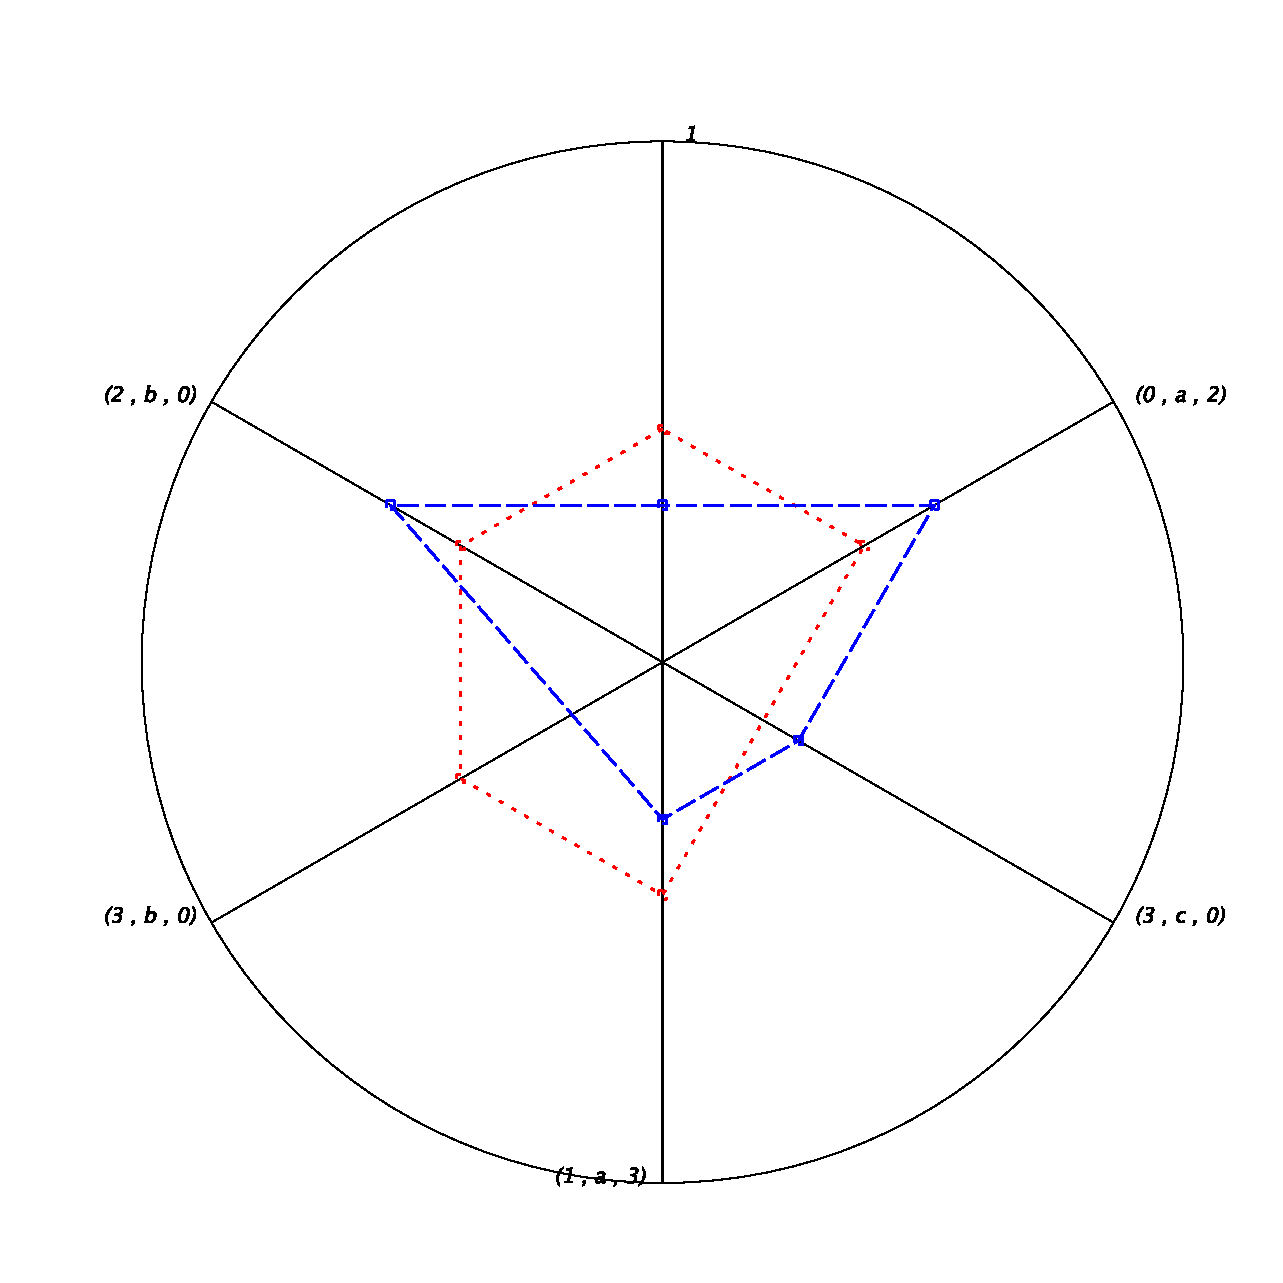
\epsfig{width=.50\textwidth,file=figures/fig-radial.eps}   
%%     \caption{Diagramme radial - Exemple}
%%     \label{fig-radial}
%% \end{figure}

%% La figure \ref{fig-radial}  est une repr\'esentation de l'espace
%% des mots pour un automate $\cal A$ sous la forme d'un diagramme
%% radial. On divise un cercle de rayon $1$ par $m+1$ rayons et
%% chaque coordonn\'ee  est repr\'esent\'ee sur le rayon
%% correspondant. Cette
%% repr\'esentation est une \og projection \fg naturelle de l'espace
%% parcouru par les vecteurs $\vec{u}$ normalis\'es plus maniable qu'une
%% projection en 2 ou 3 dimensions. Elle est rendu possible par le fait
%% que chaque coordonn\'ee est comprise entre 0 et 1. La figure
%% \ref{fig-radial} repr\'esente les diff\'erentes coordonn\'ees
%% pour le langage $a(b+c)(ab)^*$ : le trac\'e en pointill\'e
%% repr\'esente les coordonn\'ees du mot $(ab)^2$ et le
%% trac\'e en tirets le mot $ac(ab)^2$. 

%% \subsubsection{Ensemble des distances}

%% Nous supposons sans perte de g\'en\'eralit\'e que l'automate
%% $\cal A$ poss\`ede un seul \'etat terminal. L'ensemble des
%% P-vecteurs  de $L_A$, $\psi(u)$, est l'ensemble des solutions
%% dans $\N^{m+1}$ du syst\`eme d'\'equation d\'etermin\'e par la
%% matrice d'incidence de $\cal A$ :
%% $$
%% \begin{array}{cccc}
%% \left(\begin{array}{cc}
%%         1 & 0 \\
%%         S' & I 
%%     \end{array}\right)& X &=& \left(\begin{array}{cc}
%%         1  \\
%%         0 \\
%%         \vdots \\
%%         0
%%     \end{array}\right)
%% \end{array}
%% $$ 
%% o\`u $S$ est un vecteur de taille $n$ tel que $S_i=1$ si $i=q_0$ et
%% $S_i=-1$ si $i\in T$. 

%% L'ensemble $\phi(L_A)$ des
%% vecteurs  repr\'esentant les mots $u \in L_A$ est inclus dans
%% $[0,1]^{m+1}$ et il est d\'etermin\'e par 
%% l'ensemble des solutions dans $[0,1]^{m+1}$ du syst\`eme
%% d'\'equation suivant \`a coefficients dans $\mathbb{Q}$ :
%% $$
%% \begin{array}{cccc}
%% \left(\begin{array}{cc}
%%         1 & 
%%         \begin{array}{ccc}
%% 1 & \dots & 1
%% \end{array}
%% \\
%%         S' & I 
%%     \end{array}\right)& X &=& \left(\begin{array}{cc}
%%         1  \\
%%         0 \\
%%         \vdots \\
%%         0
%%     \end{array}\right).
%% \end{array}
%% $$ 

%% \subsection{$\eta$-couverture}

%% Une propri\'et\'e int\'eressante de la transposition des vecteurs
%% de $\N^{m+1}$ dans $[0,1]^{m+1}$ est de permettre de passer d'un
%% espace discret \`a un espace continu et donc de d\'efinir une
%% notion de limite pour  $\phi(u)$. Une fonction $f(x)$ poss\`ede une
%% limite $c$ en $a$ si pour tout $\epsilon > 0$, il existe $\delta > 0$ tel
%% que $\vert f(x) - c\vert < \epsilon$  quand $ 0< \vert x - a\vert <
%% \delta$. 

%% Les bornes de $\psi(u)$ forment les facettes d'un polytope convexe ouvert
%% repr\'esentant l'ensemble des  solutions de l'\'equation de $\psi(u)$. Ces sommets peuvent \^etre
%% calcul\'es par des m\'ethodes existantes de traitement des
%% polyh\`edres (voir par exemple \textsf{polylib} ou \textsf{qhull}\cite{barber96quickhull}), y compris en
%% utilisant des automates pour repr\'esenter l'ensemble des vecteurs
%% correspondant\cite{latour-auto-polyhedre}. Les bornes de $\phi(u)$
%% sont situ\'ees sur la sph\'ere en $m+1$ dimensions et sont les
%% images de l'ensemble des solutions de $\psi(u)$ par la fonction
%% $f(x)/\vert x\vert_1$. 

%% %% La partie droite de la figure \ref{fig-distance-lim} est une illustration des
%% %% propri\'et\'es de $\mathbf{s}(u,v)$ dans le cas simple de deux
%% %% dimensions. Ici, le mot $u$
%% %% est repr\'esent\'e par le vecteur $(2,1)$ et le mot $v$ par le
%% %% vecteur $(2,4)$ et l'on a donc $u=xy$ et $v=xy^4$. Dans ce cas, si on
%% %% pose $\theta = 2+i$ et $\theta'=2+4i$, on a 
%% %% $$
%% %% \vec{v} - \vec{u} = (\cos \theta' - cos\theta, \sin \theta' - \sin\theta)
%% %% $$
%% %% d'o\`u 
%% %% \begin{align}
%% %%     \mathbf{s}(u,v)^2 &= (\cos\theta' - cos\theta)^2 + (\sin
%% %%     \theta' - \sin\theta)^2 \\
%% %%     & =  \cos\theta'^{2} - 2\cos\theta'\cos\theta + \cos\theta^2 + \sin\theta'^{2} - 2\sin\theta'\sin\theta + \sin\theta^2\\
%% %%     & =  2(1 - \cos\theta'\cos\theta  - \sin\theta'\sin\theta) \label{eq:dist-mot}\\
%% %%     & =  2(1  - \cos(\theta' - \theta)) \\
%% %%     \mathbf{s}(u,v) & = \sqrt{2(1 - \cos(\theta' -
%% %%     \theta))}.
%% %% \end{align}
%% %% Si l'on consid\`ere $u=xy$ et $v=xy^k$ et en utilisant \ref{eq:dist-mot}, on a :
%% %% \begin{align}
%% %%     \lim_{k\rightarrow+\infty} \cos\theta' &= 0 \\
%% %%     \lim_{k\rightarrow+\infty} \sin\theta' &= 1 \\
%% %%     \lim_{k\rightarrow\infty} \mathbf{s}(u,v) &= 
%% %%     \sqrt{2(1-\sin\theta)}.\label{eq:lim-dist-mot}
%% %% \end{align}

%% %% \begin{figure}[htbp]
%% %% \epsfig{width=.30\textwidth,clip=,file=figures/fig-proof-triangle.eps}\hfill 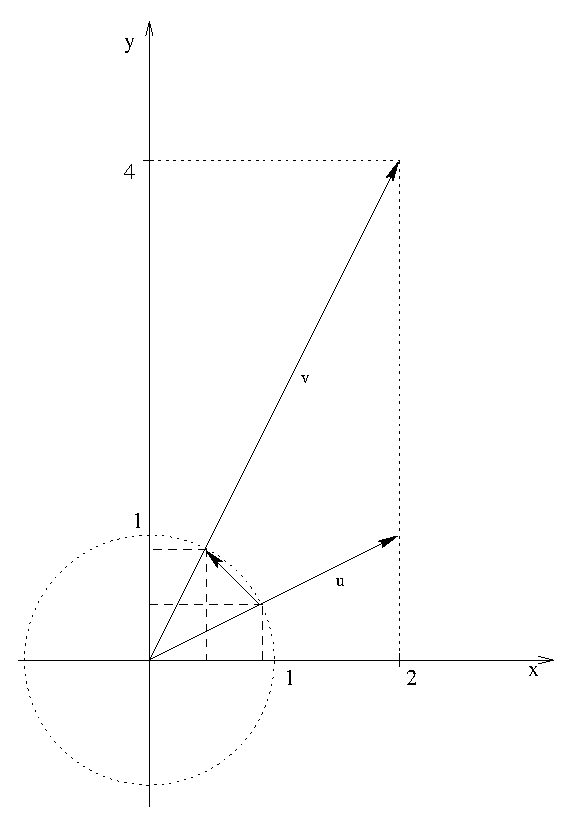
\epsfig{height=7.5cm,clip=,file=figures/fig-distance-lim.eps}
%% %%      \caption{Visualisation g\'eom\'etrique de $\mathbf{s}(u,v)$}
%% %%      \label{fig-distance-lim}
%% %% \end{figure}

%% On peut donc d\'ecrire la mani\`ere dont un
%% sous-ensemble fini du langage reconnu par $A$ \emph{couvre} le
%% langage $L$. 

%% \begin{definition}[$\eta$-couverture]
%%     Soit $T\subseteq L$ un sous ensemble des mots de $L$, $T$ est une
%%     $\eta$-couverture de $S$ si et seulement si,
%%     $$
%%     \forall u \in L, \exists t \in T, \mathbf{s}(u,t) \leq \eta.
%%     $$
%%     Clairement, $\emptyset$ est une 1-couverture de $L$ et $L$
%%     est une 0-couverture de lui-m\^eme.
%% \end{definition}

%% \begin{prop}[$\eta$-couverture]
%% Pour tout langage  $L$ reconnu par un automate $A$, pour tout
%% $\eta\in [0,1]$, il existe un langage fini $T\subseteq L$ tel
%% que $T$ est une $\eta$-couverture de $L$ : 
%% $$
%% \forall u \in L, \exists t \in T, \mathbf{s}(u,t) \leq \eta.
%% $$
%% \end{prop}

%% \begin{proof}
%% Soit $\eta$ une valeur de couverture quelconque, nous
%% construisons un ensemble fini $T$ de --- pr\'efixes de --- mots de
%% $L_A$ tel que $T$ en soit une $\eta$-couverture. 

%% Pour tout chemin \'el\'ementaire ind\'ependant $\sigma$ partant de $q_0$, l'\'etat initial
%% de $A$, on ajoute  dans $T$ le mot  $u$  construit en concat\'enant les
%% \'etiquettes des transitions composant le chemin
%% $\sigma$. Clairement, $T$ est alors une $0$-couverture de l'ensemble
%% des pr\'efixes  de mots $L_A$ ne contenant aucun facteur
%% it\'erant et c'est donc \emph{a fortiori} une $\eta$-couverture. 

%% D'apr\`es le \emph{lemme de l'\'etoile} (\cite{sakarovitch}, p.78),
%% tout mot ou facteur de mot \og suffisamment long\fg de $L_A$ contient un facteur
%% it\'erant. Soit $uv^*w$ une partie du langage de $L_A$
%% contenant un facteur it\'erant, alors d'apr\`es
%% \eqref{eq:lim-dist-mot}, on peut construire un mot
%% $y=uv^kw$ tel que pour tout $x=uv^jw \in uv^*w$, 
%% $$
%% \mathbf{s}(x,y) \leq \eta,
%% $$
%% et $T$ est donc une $\eta$-couverture de $uv^*w$. Comme
%% $L_A$ contient un nombre fini de facteurs it\'erants, $T$ est
%% fini et est donc une $\eta$-couverture de $L_A$.\hfill\qed
%% \end{proof}

%% Bien s\^ur, cette mesure de couverture est donn\'ee \emph{modulo} la
%% commutativit\'e des chemins permettant de construire des mots du
%% langage de $L_A$. Par exemple, pour le langage $(a(bc+ef)a)^*$,
%% les mots $abcaaefa$ et $aefaabca$ on m\^eme 
%% vecteur $(1,2,1,1,1,1,2)$ et sont donc \`a une distance de
%% 0. Cette commutativit\'e des chemins est induite par
%% l'ind\'ependance de certaines s\'equences de lettres, autrement dit
%% par les entrelacements d'ex\'ecution possible entre diff\'erents
%% mots. Si l'on souhaite obtenir une couverture plus fine, on peut
%% obtenir la cl\^oture commutative d'un ensemble $T$. 

%% \`A partir de cette mesure, deux questions int\'eressantes se posent :
%% \begin{enumerate}
%%   \item \'etant donn\'es un langage $L$ et un ensemble $T$, quelle est
%%     l'$\eta$-couverture de $T$ sur $L$ ? 
%%   \item \'etant donn\'es un langage reconnaissable $L$ et une
%%     couverture, $\eta$, comment g\'en\'erer un ensemble $T$ qui soit
%%     une $\eta$-couverture de $L$ ? 
%% \end{enumerate}

%% \subsubsection{Calcul de l'$\eta$-couverture de $T$}

%% L'ensemble $T\subseteq L$
%% est un ensemble fini de mots dans un langage reconnaissable donn\'e
%% repr\'esent\'e canoniquement par un automate d\'eterministe minimal
%% $\cal A$. Soit $m$ le nombre de transitions de $\cal A$, chaque mot de
%% $T$ et de $L$ est repr\'esent\'e par un vecteur de taille $m+1$ et
%% de norme 1. Par d\'efinition, la mesure de $\eta$ pour $T$ est
%% donn\'ee par la plus grande distance existant entre un mot de $T$ et
%% un mot de $L$. 

%% G\'eom\'etriquement, cette propri\'et\'e correspond \`a la
%% construction d'un \emph{diagramme de Vorono\"{\i}} \`a partir des
%% vecteurs $\phi(T)$. Pour un ensemble de
%% points $S$ dans  $\mathbb{R}^{n}$, un \emph{diagramme de
%% Vorono\"{\i}}\cite{aurenhammer-voronoi-survey} $V(S)$ est une partition de l'espace en poly\`edres
%% convexes ou \emph{r\'egions} $\mathsf{reg}(s),s\in S$ tels que que pour tout point $p\in
%% \mathsf{reg}(s)$ et pour 
%% toute r\'egion $\mathsf{reg}(s'), s\neq s'$, $d(s,p)\leq d(s',p)$. Le
%% diagramme  de Vorono\"{\i} pour $\phi(T)$ \'etant donn\'e,
%% l'$\eta$-couverture de $T$ est donn\'ee par la plus grande des
%% distances entre $t\in T$ et chacun des sommets de $\mathsf{reg}(t)$ :
%% $$
%% \eta(T) = \mathsf{max}\{ \mathbf{d}(t,p),\forall t\in T, p\in \mathsf{reg}(t)\}.
%% $$

%% L'algorithme \textsf{Quickhull}\cite{barber96quickhull} est un
%% algorithme classique et efficace de calcul d'enveloppe convexe d'un ensemble de
%% points en $n$ dimensions. Pour une dimension $d>3$ et un nombre de
%% points d'entr\'ee $n$, sa complexit\'e
%% est estim\'ee \`a $O(n^{d/2}/\lfloor d/2\rfloor!)$. Cet algorithme
%% part de la construction d'un \emph{simplex} de dimension $n$, c'est
%% \`a dire un volume r\'egulier d\'efini par $n+1$ points puis
%% il reconstruit des facettes en ajoutant un \`a un les points de
%% l'ensemble d'entr\'ee et en trouvant la facette la plus proche du
%% point ajout\'e pour la diviser. 

%% \subsubsection{Calcul de $T$ en fonction de l'$\eta$-couverture}

%% Le calcul de $T$ en fonction de $\eta$ est le dual du probl\`eme
%% pr\'ec\'edent. Si l'on reprend la d\'efinition d'$\eta(T)$
%% donn\'ee ci-dessus, on constate que cette d\'efinition d\'epend de
%% la construction d'un ensemble de r\'egions dont la plus grande
%% distance est inf\'erieure ou \'egale \`a $\eta$. Pour construire
%% $T$, on va donc tout d'abord construire un 
%% polytope convexe r\'egulier dont toutes les r\'egions ont m\^eme
%% diam\`etre, en l'occurrence $\eta$, par subdivision du simplex de base correspondant
%% aux limites pour le langage $L$ dans chacune des dimensions. 

%% On obtient ainsi les coordonn\'ees d'un
%% ensemble de vecteurs, le centre de chaque facette du polytope,
%% repr\'esentant les candidats pour $T$. 
%% L'espace
%% vectoriel construit \`a partir de l'automate $A$ repr\'esentant $L$ est
%% particulier en ceci que tous les vecteurs que l'on peut d\'efinir ne
%% sont pas des mots de $L$ : seuls les vecteurs correspondant \`a une
%% s\'equence de transitions depuis l'\'etat initial de $A$ sont
%% valides. Il est donc fort possible qu'en construisant le polytope
%% \`a partir de $\eta$, certaines parties de celui-ci ne puissent
%% \^etre mis en correspondance avec des mots de $L$, et ce pour deux
%% raisons diff\'erentes :
%% \begin{itemize}
%%   \item soit le vecteur  ne permet pas de
%%   reconstruire un vecteur avec des coefficients entiers appartenant
%%   \`a $\psi(u)$, auquel cas il
%%   est n\'ecessaire de choisir des approximations raisonnables des
%%   coefficients calcul\'es pour retrouver le mot r\'eel ;
%% \item soit le vecteur est dans une r\'egion ne pouvant contenir aucun
%%   mot par construction. 
%% \end{itemize}
%% Pour r\'esoudre le premier cas, on va construire un poly\`edre \`a
%% partir d'une valeur plus petite de $\eta$ nous garantissant \emph{in
%%   fine} la propri\'et\'e attendue d'une $\eta$-couverture : en
%% choisissant $\frac{\eta}{2}$ comme diam\`etre maximal des facettes du
%% poly\`edre, on est s\^ur que si un mot existe sur l'arc
%% correspondant \`a cette ar\^ete, il sera \`a une distance
%% inf\'erieure ou \'egale \`a $\eta$ des mots sur les arcs des
%% ar\^etes adjacentes. 

%% Le second cas d'impossibilit\'e de reconstruction de mots ne peut
%% \^etre r\'esolu qu'en identifiant les r\'egions d'arcs
%% correspondant \`a chaque sommet et en choisissant des mots les plus
%% proches possibles de cette fronti\`ere.

%% Un polytope dont tous les sommets sont situ\'es sur la surface d'une
%% sph\`ere est appel\'e sph\`ere g\'eod\'esique car les ar\^etes
%% reliant chaque sommet sont des g\'eod\'esiques de la sph\`ere
%% consid\'er\'ee. La construction d'un polytope de dimension $n$ tel que la distance
%% entre deux sommets adjacents soit toujours inf\'erieure \`a
%% $\frac{\eta}{2}$ est algorithmiquement complexe. Succintement, le
%% principe de l'algorithme consiste \`a construire incr\'ementalement
%% le polytope par divisions de ses facettes. 

%% \subsection{Approximation de l'$\eta$-couverture}

%% Il appert de la discussion pr\'ec\'edente que le calcul de la
%% solution exacte aux deux probl\'emes que nous avons soulev\'e est
%% loin d'\^etre triviale et qu'elle est de plus algorithmiquement
%% co\^uteuse. De mani\`ere assez \'evidente, elle cro\^{\i}t  exponentiellement avec le nombre de
%% transitions de l'automate que l'on cherche \`a caract\'eriser. Dans
%% une optique pragmatique de s\'election de cas de tests pertinents, nous nous contenterons donc d'une
%% approximation de la notion d' $\eta$-couverture qui soit effectivement
%% calculable en temps raisonnable. Cette approximation sera
%% calcul\'ee incr\'ementalement lors du processus d'ex\'ecution et de
%% s\'election des cas de tests et l'algorithme correspondant sera
%% d\'etaill\'e dans la section suivante.


%% %% \paragraph{Sph\`ere g\'eod\'esique}

%% %% Une sph\`ere g\'eod\'esique est un poly\`edre dont  tous les sommets sont situ\'es
%% %% sur une sph\`ere. La construction d'une telle structure est un
%% %% probl\`eme classique en g\'eom\'etrie et a des applications
%% %% \'evidentes en informatique graphique. 

%% %% Nous adaptons ici un algorithme de construction r\'ecursive d'une
%% %% sph\`ere g\'eod\'esique dont le nombre de facettes est fix\'e,
%% %% au probl\`eme de construction d'une portion de sph\`ere
%% %% g\'eod\'esique de rayon 1 param\'etr\'ee par la longueur des
%% %% ar\^etes de chaque facette. L'algorithme est d\'etaill\'e dans la figure
%% %% \ref{fig-algo-geodesique} qui d\'efinit une fonction r\'ecursive
%% %% contr\^ol\'ee par une certaine valeur de $\eta$. Le principe de
%% %% l'algorithme est simple :
%% %% \begin{itemize}
%% %%   \item on part d'une facette unique dont les sommets sont les
%% %%     extr\'emit\'es des vecteurs base de l'espace --- une sph\`ere de
%% %%     dimension $n$ ;
%% %%   \item r\'ecursivement, on d\'ecoupe chaque facette de l'ensemble
%% %%   courant en un certain nombre de facettes en ajoutant des points :
%% %%   \begin{itemize}
%% %%     \item pour chaque segment de la facette, on ajoute le point m\'edian
%% %%       si la longueur de l'ar\^ete est sup\'erieure \`a $\eta$,
%% %%     \item on ajoute le barycentre de la facette si au moins deux
%% %%     sommets non-adjacents de la facette sont \`a une distance
%% %%     sup\'erieur \`a $\eta$. 
%% %% \end{itemize}
%% %% Les vecteurs correspondant aux nouveaux points ajout\'es sont
%% %% \emph{normalis\'es} pour construire des points sur la surface de la
%% %% sph\`ere et chaque triplet de points constitue une nouvelle facette. 
%% %% \end{itemize}



%% %% Pour
%% %% le m\^eme alphabet, l'\emph{application de matrice de
%% %% Parikh}\cite{tucs-parikh-matrix,egecioglu-qmatrix-parikh} est un morphisme
%% %% $\Psi_{\mathfrak{M}_k}$ de $\Sigma^*$ dans $\mathbf{N}^{k+1
%% %%   \times{}k+1}$, l'ensemble des matrices carr\'ees \`a coefficients
%% %% entiers de dimension $k+1$. Pour toute letter $a_q\in \Sigma$, on a
%% %% $\Psi_{\mathfrak{M}_k}(a_q) = M^{k+1,k+1}$ avec :
%% %% $$
%% %% m_{i,j} = 
%% %% \left\{\begin{array}{ll}
%% %% 1,&\mbox{si~} i=j, \\
%% %% 1,&\mbox{si~} i=q et j=q+1, \\
%% %% 0,& \mbox{~sinon}.
%% %% \end{array}\right.
%% %% $$
%% %% et pour $\Sigma^*$, on a :
%% %% $$
%% %% \begin{array}{rl}
%% %% \Psi_{\mathfrak{M}_k}(\epsilon) & = \mathbf{1}^{k+1,k+1} \\
%% %% \Psi_{\mathfrak{M}_k}(u.a) &=
%% %% \Psi_{\mathfrak{M}_k}(u)\Psi_{\mathfrak{M}_k}(a). 
%% %% \end{array}
%% %% $$
%% %% Une \emph{matrice de Parikh} est ainsi une matrice triangulaire
%% %% sup\'erieure de dimension $k+1$ dont la principale propri\'et\'e
%% %% est de compter des occurences de sous-mots : 
%% %% $$
%% %% m_{i,j+1}(w) = \vert w\vert_{a_{i,j+1}},\mbox{~pour tout~} 1\leq i\leq j\leq k,
%% %% $$
%% %% avec $\vert w\vert_u$ d\'enotant le nombre d'occurences de $u$ comme
%% %% sous-mot de $w$ et $a_{i,j}$ pour $i<j$ d\'enotant le mot
%% %% $a_ia_{i+1}\dots a_j$. En particulier, la seconde diagonale d'une
%% %% matrice de Parikh d'un mot $u$ est le vecteur de Parikh de ce mot $u$.

 
%% %% Par \eqref{eq:lim-dist-mot}, on a
%% %% $$
%% %% \eta = \sqrt{2(1 -  \sin \theta)}
%% %% $$
%% %% avec $\sin\theta = x_i$ d'o\`u
%% %% \begin{align*}
%% %%     \sin\theta &= 1 - \frac{\eta^2}{2} \\
%% %%     \theta &= \sin^{-1}(1 - \frac{\eta^2}{2}),
%% %% \end{align*}
%% %% d'o\`u on d\'eduit le nombre de points du poly\`edre pour un couple
%% %% de coordonn\'ees, 
%% %% $$n=\left\lfloor\frac{\pi}{2(\frac{\pi}{2} -\theta)}\right\rfloor$$, et donc les
%% %%  $n$ coordonn\'ees 
%% %% $$
%% %% (\cos\theta,\sin
%% %% \theta),(\cos(2\theta-\frac{\pi}{2}),\sin(2\theta-\frac{\pi}{2}),
%% %% \dots, (\cos((n+1)\theta-\frac{n\pi}{2}),\sin((n+1)\theta-\frac{n\pi}{2}).
%% %% $$



%% %% \paragraph{Nombre de mots de taille $n$ dans un automate
%% %%   d\'eterministe}

%% %% \begin{quote}
%% %%     D'apr\`es \cite{sakarovitch} (p.229) et \cite{chomsky-finite-sl}.
%% %% \end{quote}

%% %% Soit $A=(Q,q_0,T,\Sigma,\delta)$ un automate d\'eterministe. On
%% %% d\'efinit la matrice $M \in \mathbb{N}^{Q\times{}Q}$ dont les
%% %% coefficients sont indic\'es  par les \'etats de $A$ et sont
%% %% d\'efinies comme : 
%% %% $$
%% %% m_{p,q} = \vert \{ (p,a,q) \in \delta \}\vert.
%% %% $$ 
%% %% Le nombre de facteurs droit du langage de $A$ de taille $n+1$
%% %% reconnaissables \`a partir de $q$, $L_q(n+1)$ est d\'efini par la relation de
%% %% r\'ecurrence :
%% %% $$
%% %% L_q(n+1) = \sum_{q\in Q} m_{p,q}l_q(n),
%% %% $$
%% %% et donc pour tous les \'etats de $Q$, on obtient l'\'equation
%% %% matricielle 
%% %% $$
%% %% \vec{l}(n+1) = M\vec{l}(n) = M^{n+1}\vec{l}(0),
%% %% $$
%% %% o\`u les coefficients du vecteur $\vec{l}(k)$ sont les $l_q(k)$, pour
%% %% chaque $q\in Q$. Pour $\vec{l}(0)$, on a 
%% %% $$
%% %% l_p(0) = \left\{
%% %%     \begin{array}{ll}
%% %% 1,&\mbox{~si $p\in T$~},
%% %% 0, \mbox{~sinon~}.
%% %%     \end{array}\right.
%% %% $$

%% %% Soit $P(\lambda) = \mathrm{det}(M-\lambda I) = (-1)^k(\lambda^k -
%% %% z_1\lambda^{k-1} - \dots -z_{k-1}\lambda - z_k)$ le polyn\^ome
%% %% caract\'eristique de la matrice $M$, alors on a :
%% %% $$
%% %% P(M) = 0.
%% %% $$

%% %% Par exemple, soit l'automate de la figure
%% %% \ref{fig-sample-dfa-distance}, 
%% %% on a le syst\`eme d'\'equations suivants :
%% %% \begin{align*}
%% %%     l_3(n) &= l_0(n-1) \\
%% %%     l_0(n) &= 2l_2(n-1) \\
%% %%     l_2(n) &= l_1(n-1) \\
%% %%     l_1(n) &= l_2(n-1). \\
%% %% \end{align*}
%% %% Avec 
%% %% $$
%% %% M=\left(
%% %%     \begin{array}{cccc}
%% %% 0 & 0 & 2 & 0 \\ 
%% %% 0 & 0 & 1 & 0 \\
%% %% 0 & 1 & 0 & 0 \\
%% %% 1 & 0 & 0 & 0 
%% %%     \end{array} \right), 
%% %% $$
%% %% d'o\`u l'on d\'eduit le polyn\^ome caract\'eristique 
%% %% $$
%% %% P(\lambda) = 24\lambda^2 -16\lambda +12,
%% %% $$
%% %% ce qui nous donne la relation 
%% %% $$
%% %% L(n) = 
%% %% $$

%% %% \begin{floatingfigure}{.5\textwidth}
%% %%     \centering
%% %% \begin{lstlisting}[linewidth=.45\textwidth,mathescape=true,literate={:=}{{$\leftarrow$}}1 ]
%% %% Input:  $G=(S,E)$ un graphe dirig\'e
%% %%         $s_0$ \'etat initial distingu\'e  de $G$
%% %% Output: $C$ un ensemble de chemins \'el\'ementaires
%% %% C := $\emptyset$
%% %% // $G'=(S',A')$ is covering tree for $G$
%% %% G' := covering(G)
%% %% for each $(s,s') \in A\setminus A'$
   
%% %% \caption{Base de cycles d'un graphe dirig\'e $G=(S,E)$}
%% %% \label{fig-algo-cyclebase}
%% %% \end{floatingfigure}


%% \section{Algorithmes}

%% \subsection{Jeu \`a deux joueurs}
%% \label{sec:jeu-deux-joueurs}
%% Le test peut \^etre vu comme un jeu \`a deux joueurs : le \emph{testeur} et
%% l'\emph{implantation}. Le testeur \og gagne\fg le jeu s'il pouse
%% l'implantation \`a la faute, c'est \`a dire s'il observe dans son
%% interaction avec l'implantation une ex\'ecution non conforme \`a la
%% sp\'ecification, quel que soit le sens pr\'ecis donn\'e au mot
%% \emph{conforme}. Par sym\'etrie, l'implantation \og gagne\fg  si elle
%% ne produit pas d'ex\'ecution non conforme, ou si le testeur abandonne
%% la partie. Cette vision des choses a donn\'e lieu \`a un certains
%% nombres de travaux d\'ej\`a cit\'es dans le chapitre
%% \ref{chap-etatarttest}, section \ref{sec:selection-iolts}. 

%% Dans un tel contexte, la question est de d\'efinir le comportement
%% des deux joueurs, c'est \`a dire leurs \emph{strat\'egies} :
%% celle-ci peut \^etre fixe ou adaptative. Dans le domaine de la
%% th\'eorie des jeux, on parlera aussi  de strat\'egie \emph{pure}, \emph{mixte} ou
%% \emph{comportementale}. 

%% Formellement, un jeu \`a deux joueurs
%% $\mathsf{G}(\mathsf{P},\mathsf{O})$, o\`u $\mathsf{P}$ ---
%% \emph{player} -- et $\mathsf{O}$  --- \emph{opponent} --- d\'esignent
%% chacun des adversaires, peut \^etre d\'efini comme un graphe biparti dans
%% lequel les n\oe uds repr\'esentent des \emph{positions} ou
%% configurations de jeux et les transitions des \emph{coups}. Une
%% position initiale est distingu\'ee dans l'ensemble des positions
%% possibles et deux positions distingu\'ees, not\'ees $\mathsf{W}$ ---
%% \emph{win} --- et $\mathsf{L}$ --- \emph{lose} --- terminent toute
%% partie. 

%% Autrement dit, si l'ensemble des positions est fini un jeu est
%% un automate d'\'etat fini $\mathsf{G}=(Q,q_0,T,\Sigma,\delta)$ dans
%% lequel :
%% \begin{itemize}
%%   \item $Q = Q_\mathsf{O} \cup Q_\mathsf{P} \cup \{W,L\}$ l'ensemble des \'etats est partitionn\'e en
%%     en trois sous-ensembles repr\'esentants respectivement les
%%     positions de $\mathsf{O}$, de $\mathsf{P}$ et les positions gagnantes et perdantes
%%     pour $\mathsf{P}$ ;
%%   \item $q_0\in Q$ est la position initiale du jeu ;
%%   \item $T=\{W,L\}$ est l'ensemble des \'etats terminaux du jeu ;
%%   \item $\Sigma=\Sigma_\mathsf{O} \cup \Sigma_\mathsf{P}$  est
%%   l'ensemble des coups partitionn\'e en deux sous-ensembles
%%   repr\'esentant les coups de $\mathsf{O}$ et $\mathsf{P}$ ;
%% \item et $\delta\subseteq (Q_\mathsf{O} \times{}\Sigma_\mathsf{O} \times{}
%%   (Q_\mathsf{P}\cup T)) \cup (Q_\mathsf{P} \times{}\Sigma_\mathsf{P} \times{}
%%   (Q_\mathsf{O}\cup T))$ est la relation de transition repr\'esentant
%%   les diff\'erents coups possibles en fonction des positions.
%% \end{itemize}

%% Une \emph{strat\'egie pure} ou pr\'efix\'ee  $\mathbf{s}$ pour $\mathsf{P}$ --- resp. pour
%%  $\mathsf{O}$ ---  est une application de
%%  $Q_\mathsf{P}$ dans $\Sigma_\mathsf{P}$ --- resp. $Q_\mathsf{O}$ dans $\Sigma_\mathsf{O}$.
%% Une strat\'egie \emph{comportementale} ou adaptative est une
%% application de $\Sigma^* \times{}Q_\mathsf{P}$ dans
%% $\Sigma_\mathsf{P}$. Une strat\'egie peut \^etre d\'eterministe ou
%%  probabiliste : dans ce dernier cas, $\mathbf{s}$ est une
%%  \emph{relation} \`a laquelle on associe une distribution de
%%  probabilit\'e $p$ telle que $\forall q\in Q_\mathsf{P},\sum_{a\in
%%  \Sigma_\mathsf{P}} p(\mathbf{s}(q)) = 1$, respectivement $\forall
%%  q\in Q_\mathsf{P},h\in \Sigma^*,\sum_{a\in
%%  \Sigma_\mathsf{P}} p(\mathbf{s}(q,h)) = 1$. 

%% Plus simplement, une strat\'egie pure est fix\'ee 
%% une fois pour toute avant le d\'emarrage du jeu et le joueur
%% ex\'ecutera ses coups de mani\`ere d\'eterministe en fonction de la
%% position courante. Une strat\'egie
%% adaptative permet, comme son nom l'indique, au joueur de s'adapter non
%% seulement \`a la position courante, mais aussi \`a la s\'equence de
%% coups ayant permis d'atteindre cette position. 

%% Une \emph{strat\'egie gagnante} pour $P$ est une strat\'egie telle que
%% toutes les s\'equences de coups possibles m\`enent \`a l'\'etat
%% $W$. La question de l'existence d'une strat\'egie gagnante et de sa
%% construction dans diff\'erentes situations de test est
%% synth\'etis\'ee dans \cite{yannakakis-test-opt-games}. Il est clair
%% que dans tous les cas int\'eressants, la construction d'une
%% strat\'egie gagnante \emph{a priori} est trop complexe pour \^etre
%% faisable. 

%% L'algorithme classique du \textsc{Minimax} et sa version \'evolu\'ee l'algorithme
%% \emph{alpha-beta}\cite{rich-ai} offrent une r\'eponse partielle \`a ce
%% probl\`eme. Les coups du joueur $\mathsf{P}$ sont choisis en
%% fonction d'une exploration partielle des diff\'erentes \'evolutions
%% possibles de la position courante, le coup jou\'e \'etant choisi en
%% fonction d'une heuristique d'\'evaluation $\mathbf{v}: \Sigma^* \times{}Q
%% \rightarrow [-1,1]$ respectant les r\`egles suivantes :
%% \begin{itemize}
%%   \item $\mathbf{v}(L) = -1$ et $\mathbf{v}(W) = 1$ ;
%%   \item $v(q,h) \leq 0$ si $q\in Q_\mathsf{O}$ et $v(q,h) \geq 0$ si
%%     $q\in Q_\mathsf{P}$.
%% \end{itemize}

%% L'int\'er\^et de l'algorithme \emph{alpha-beta} par rapport \`a une recherche
%% classique  de type \textsc{Minimax} est d'utiliser des valeurs seuils,
%% $\alpha$ et $\beta$ permettant d'\'elaguer l'arbre de recherche et
%% donc d'accro\^{\i}tre la profondeur de recherche pour un m\^eme temps de traitement. 

%% \subsection{Jeu \& Test}

%% Cet algorithme forme la base d'une \emph{strat\'egie adaptative} pour
%% le joueur $\mathsf{P}$, c'est \`a dire dans notre contexte pour le
%% \emph{testeur}. Le probl\`eme principal consiste donc \`a construire
%% la fonction $\mathbf{v}:\Sigma^* \times{}Q \rightarrow [-1,1]$
%% d'\'evaluation pour $\mathsf{P}$.

%% Pour ce qui concerne $\mathsf{O}$, c'est \`a dire dans notre contexte
%% l'implantation test\'ee, sa \og strat\'egie\fg ou son comportement,
%% sont par d\'efinition inconnus et c'est le but du test de les
%% d\'ecouvrir. Toutefois, pour les besoins de la fonction
%% d'\'evaluation, il est n\'ecessaire au joueur $\mathsf{P}$ d'estimer
%% la valeur de chacune des diff\'erentes positions du point de vue de
%% l'adversaire, c'est \`a dire de d\'efinir un mod\`ele de
%% comportement de l'implantation test\'ee. Diff\'erents mod\`eles
%% sont possibles :
%% \begin{itemize}
%%   \item un mod\`ele \emph{pessimiste} o\`u $\mathsf{O}$ est suppos\'e
%%     avoir pour strat\'egie de \og dissimuler\fg les d\'efauts ;
%%   \item un mod\`ele optimiste ou coop\'eratif o\`u $\mathsf{O}$
%%   coop\`ere avec $\mathsf{P}$ pour d\'ecouvrir les \'eventuels
%%   d\'efauts ;
%% \item et un mod\`ele neutre o\`u le comportement de $\mathsf{O}$ est
%%   al\'eatoire. 
%% \end{itemize}

%% Le choix d'un mod\`ele d\'epend des hypoth\`eses faites sur les
%% d\'efauts et erreurs pr\'esents dans l'implantation et donc en
%% dernier ressort d'hypoth\`eses sur le comportement du programmeur
%% ayant r\'ealis\'e l'implantation test\'ee. 

%% \subsection{Algorithme de base}
%% \label{sec:algorithme-de-base}
%% \`A partir des \'el\'ements d\'efinis ci-dessus, nous d\'etaillons
%% dans cette section l'algorithme de s\'election et d'ex\'ecution des
%% cas de tests pour les automates \textsf{FIDL}. Dans un premier temps,
%% nous supposerons que l'automate repr\'esente bien un langage
%% reconnaissable sur un alphabet fini. 
%% Nous supposerons par
%% ailleurs que la sp\'ecification est constitu\'ee d'un
%% unique automate \textsf{FIDL}, \'eventuellement non d\'eterministe
%% et incomplet mais dont le langage est \emph{bien-form\'e} : les mots du
%% langage de l'automate sont une alternance d'entr\'ees et de sorties.
%% L'algorithme de base est donn\'e dans la figure
%% \ref{fig-algo-test-base}. Cet algorithme est globalement similaire \`a celui
%% pr\'esent\'e dans \cite{kervinen-heuristic}.


%% \subsubsection{Fonction d'\'evaluation}

%% Le c\oe ur du processus de s\'election est constitu\'e par la fonction
%% \textsf{eval} d\'etaill\'ee dans la figure
%% \ref{fig-algo-eval}. \textsf{eval} est une
%% instance de l'algorithme
%% \emph{alpha-beta} pr\'esent\'e ci-dessus qui  lance l'exploration
%% des transitions de l'automate pour \'evaluer la position courante en
%% fonction de ses d\'eveloppements possibles. 

%% Cette fonction est r\'ecursive, la profondeur de r\'ecursion
%% \'etant contr\^ol\'ee par le param\`etre de profondeur
%% \textsf{depth}. Lorsque la profondeur maximale est atteinte (ligne
%% 11), la fonction retourne simplement l'\'evaluation de la position
%% courante comme le minimum de la distance entre la trace courante et
%% l'ensemble de test, affect\'e d'un signe positif si l'on se trouve
%% dans une position de $Q_O$ et n\'egatif sinon.

%% Sinon, l'\'evaluation proc\`ede r\'ecursivement par \'evaluation
%% des diff\'erentes traces possibles \`a partir de la position
%% courante. Les valeurs de $\alpha$ et de $\beta$ contr\^olent la
%% mani\`ere dont l'\'elagage op\`ere (lignes 23 et 36) : 
%% \begin{itemize}
%%   \item dans une position o\`u c'est \`a l'adversaire de jouer, si
%%   la plus petite \'evaluation d\'ej\`a effectu\'ee est
%%   inf\'erieure \`a la borne $\alpha$, alors l'exploration
%%   s'arr\^ete sur cette valeur : en effet, dans ce cas, toute autre
%%   \'evaluation sera au moins aussi bonne du point de vue de
%%   l'adversaire et donc npire du point de vue du joueur et il n'est
%%   donc pas n\'ecessaire de poursuivre l'exploration ;
%% \item dans une position o\`u c'est au testeur de jouer, l'\'elagage
%%   s'effectue \'evidemment pour une \'evaluation qui est plus grande
%%   que la borne $\beta$. 
%% \end{itemize}

%% \begin{figure}[htbp]
%%     \centering
%% \begin{lstlisting}[linewidth=\textwidth,mathescape=true,numbers=left,numberstyle=\tiny,literate={:=}{{$\leftarrow$}}1 ]
%% function eval(S,q,Trace,T,$\alpha$,$\beta$, depth)
%% Input : $S=(Q,q_0,\Sigma,\delta)$
%%         $q\in Q$
%%         $T \subset L_S$ 
%%         Trace $\in L_S$       
%%         $\alpha,\beta \in \mathbb{R}$
%%         depth $\in \mathbb{N}$ 
%% Output : 
%%         val $\in \mathbb{R}$

%% if depth = 0
%%    if $q \in Q_\mathsf{O}$
%%       return min($\{d(u,Trace) \mid u \in T\}$)
%%    else
%%       return -min($\{d(u,Trace) \mid u \in T\}$)
%% if $q \in Q_\mathsf{O}$ 
%%    m := $\beta$
%%    for each $(q,a,q') \in \delta$ 
%%       t := eval(S,q',Trace.a,T,$\alpha$,m,depth - 1)
%%       if t < m 
%%         m := t
%%       end
%%       if m $\leq$ $\alpha$ 
%%          return m 
%%       end 
%%    end
%%    return m
%% else 
%% if $q\in Q_\mathsf{P}$ 
%%    m := $\alpha$
 %%    for each $(q,a,q') \in \delta$
%%       t := eval(S,q',Trace.a,T,m,$\beta$, depth - 1)
%%       if t > m 
%%         m := t
%%       end
%%       if m $\geq$ $\beta$ 
%%          return m 
%%       end 
%%    end   return m
%% end
%% \end{lstlisting}
%% \caption{Fonction d'\'evaluation}
%% \label{fig-algo-eval}
%% \end{figure}

%% \subsubsection{Estimation de la strat\'egie de l'adversaire}

%% La proc\'edure \textsf{eval} est bas\'ee sur l'hypoth\`ese que les
%% strat\'egies des deux joueurs sont concurrentes et donc qu'une bonne
%% \'evaluation pour l'adversaire est mauvaise pour le joueur et
%% inversement. Le jeu est consid\'er\'e comme \'etant un jeu \`a
%% somme nulle et la strat\'egie d'\'evaluation de l'adversaire est une
%% strat\'egie \emph{pessimiste} : on consid\`ere que l'\textsf{IUT} va
%% chercher \`a minimiser la couverture atteinte. Cette hypoth\`ese
%% revient \`a favoriser les comportements r\'ep\'etitifs de
%% l'\textsf{IUT}.

%% \section{Test d'automates synchronis\'es}

%% Un composant \textsf{FIDL} est g\'en\'eralement mod\'elis\'e \`a
%% l'aide de plusieurs automates  compos\'es par un produit de
%% synchronisation. Or nous avons dans la section pr\'ec\'edente
%% consid\'er\'e uniquement le cas d'un processus de test par rapport
%% \`a un et un seul automate, qui plus est consid\'er\'e comme
%% d\'eterministe est bien form\'e. Dans le cas d'un composant, cette
%% situation n'est pas tr\`es r\'ealiste : d'une par les automates
%% consid\'er\'es sont rarement d\'eterministes, d'autre part leur
%% composition par produit de synchronisation introduit
%% g\'en\'eralement de l'entrelacement entre les messages d'entr\'ee
%% et de sorties du composant. 

%% Cette situation est similaire au probl\`eme du test r\'eparti, dans
%% sa version synchronis\'ee (voir chapitre \ref{chap-etatarttest}). Les
%% points de contr\^ole et d'observation sont ici les diff\'erents
%% ports du composant. De plus, les synchronisations entre ports sont
%% connues, au moins partiellement, par la sp\'ecification du
%% comportement du composant au moyens d'automates.

%% \subsection{R\`egles du jeu}

%% Nous choisissons toujours de mod\'eliser le processus comme un jeu
%% entre deux joueurs. La principale diff\'erence est que d\'esormais,
%% les deux joueurs jouent simultan\'ement plusieurs jeux dont les coups
%% ne sont pas disjoints.
 

%% %% \subsection{Test execution}
%% %% \label{sec-test-execution}

%% %% Following \cite{gametest}, we will model this process $T$ as a
%% %% two-player game between a specification $S$ and a component under test
%% %% $C$. The "game board" is the current set of input and output messages
%% %% $(i,o)$, with $i$ and $o$ subsets of $I$ and $O$, respectively. Players
%% %% alternate turns by adding or removing elements from the game board
%% %% under the following rules:
%% %% \begin{enumerate}
%% %%   \item A play from $C$ consists in removing all the available
%% %%     messages from $i$ --- \emph{i.e.}  consuming inputs and adding
%% %%     messages to $o$ --- \emph{i.e.} producing outputs,
%% %%   \item $S$ plays the reverse game, thus removing all available
%% %%     messages in $o$ and producing messages in $i$,
%% %%   \item It is assumed that $S$ always begin the game --- \emph{i.e.}
%% %%     the component is \emph{reactive} to its environment. This
%% %%     assumption is not really an issue as we could equally apply our
%% %%     test procedure to an already existing output set.
%% %% \end{enumerate}
%% %% Each game play is thus a --- possibly infinite --- sequence of game
%% %% board configurations with both sides alternating play
%% %% $$
%% %% (\emptyset,\emptyset) \xrightarrow{S} (i_1,\emptyset) 
%% %% \xrightarrow{C} (\emptyset,o_2) \dots \xrightarrow{S}
%% %% (i_{n-1},\emptyset) \xrightarrow{C} (\emptyset,o_n). 
%% %% $$

%% %% The moves of $S$ are controlled by the FIDL automata the
%% %% specification relies on and so each play from $S$ must follow the
%% %% following rules with a game board $(\emptyset,o)$, when ${\mathcal A}$
%% %% is in state $(q,\sigma)$:
%% %% \begin{enumerate}
%% %% \item Find a word $u$ such that 
%% %%   $${\cal A} : q \xrightarrow{u} q',$$
%% %%   and such that the set of
%% %%   occurrencies of letters of $O$ used in $u$ is equal to $o$ (that is
%% %%   the set of output letters contained in $u$ is the same as the output
%% %%   letters produced by $C$ in $o$),
%% %% \item We
%% %%   define $i'$ the new input set as the set of occurrencies of letters
%% %%   of $I$ of $u$. Then the new game board is $(i',\emptyset)$ and the
%% %%   automata makes progress to new state $(q',\sigma')$,
%% %% \item If $i'$ is empty following step 2, then find a word $w$ such
%% %% that  
%% %% $${\cal A} : q' \xrightarrow{w} q'',$$
%% %% and such that $w$ does not
%% %% contain any output, define the new input set as the letters of $w$
%% %% and update the state of ${\cal A}$ to $(q'',\sigma'')$.
%% %% \end{enumerate}
%% %% % \begin{enumerate}
%% %% % \item Find a word $u=a_1 a_2 \dots a_n$ such that 
%% %% % $${\cal A} : q \xrightarrow{u} q',$$ and 
%% %% % $$\Pi_O (u) = o,
%% %% % $$
%% %% % that is the set of output letters contained in $u$ is the same as the
%% %% % output letters produced by $C$ in $o$,
%% %% % \item given the current state of $\cal A$, defined as $(q,\sigma)$,
%% %% % we define $i'$ the new input set as 
%% %% % $$
%% %% % i' = \{ a \in \Pi_I(u) \},
%% %% % $$
%% %% % then the new board game is $(i',\emptyset)$ and the automata makes
%% %% % progress to new state $(q',\sigma')$,
%% %% % \item if $i'$ is empty following step 2, then find a word $w$ such
%% %% % that 
%% %% % $${\cal A} : q' \xrightarrow{w} q'',$$ and 
%% %% % $$\Pi_O(w) =\emptyset,$$
%% %% % define the new input set as $w$ and update the state of ${\cal A}$ to
%% %% % $(q'',\sigma'')$. 
%% %% % \end{enumerate}

%% %% If $S$ cannot make any move, either by not being able to consume an output
%% %% message or being in a state with no possible input message to
%% %% generate and no output message to consume, then the game ends and $S$
%% %% \emph{wins}, that is a defect has been found in the implementation.
%% %% The play of $C$ is of course controlled by the internal implementation
%% %% of the component under test, which is by definition unknown and the
%% %% game ends when one of the following happens: 
%% %% \begin{itemize}
%% %% \item $S$ wins by the preceding rules, \emph{i.e.} it cannot play, 
%% %% \item A sequence of moves is repeated infinitely often: this is a
%% %% winning game for $C$.
%% %% \end{itemize}

%% %% We must stress that in practice, victory conditions for both players
%% %% are usually asserted using external assumptions, for example by giving
%% %% timeout values for output generation and upper bounds for loops. 

%% %% These rules model a \emph{conformance relation}
%% %% between $S$ and $C$ such that, given any configuration --- \emph{i.e.}
%% %% any state of the implantation and the specification:
%% %% \begin{itemize}
%% %% \item The implantation must accept all correct inputs,
%% %% \item And it may not generate more outputs than specified.
%% %% \end{itemize}

%% %% Given such model, we define a new automaton known as \emph{test purpose} 
%% %% to drive the test game and help the tester generate inputs and
%% %% consume outputs.



%% \subsubsection{Variables \& Donn\'ees}

%% \subsection{Application au test de composants \textsf{FIDL}}

%% \subsubsection{Test de ports}



%% \subsubsection{Testeurs}

%% Un testeur a donc pour fonction d'interagir avec l'IUT, autrement dit
%% un \emph{composant}, les testeurs de ports  d\'ecrits ci-dessus
%% n'ayant pas la possibilit\'e dans notre contexte d'exister de
%% mani\`ere autonome : un port n'existe  pas en l'absence de composant. Pour que
%% cette interaction est un sens, il faut bien \'evidemment que le
%% testeur et l'IUT \emph{puissent} interagir, ce qui dans notre contexte
%% signifie que le testeur et l'IUT peuvent \^etre \emph{connect\'es}
%% l'un \`a l'autre.  Ceci nous am\`ene  donc naturellement \`a
%% d\'efinir un testeur pour un --- type de --- composant donn\'e comme
%% un autre composant poss\'edant certaines caract\'eristiques :

%% \begin{definition}[Testeur]
%%     Un \emph{testeur} $T_C$ pour un composant  $C = \langle Port(C),
%%     \Tr(C) \rangle$ est lui m\^eme un composant $T_C = \langle
%%     Port(T_C),\Tr(C)\rangle$ tel que 
%%     pour chaque port de $Port(C)$ il existe un port
%%     connectable dans $T_C$ :
%%     $$
%%     \begin{array}{rcl}
%%         Port(T_C) &=& \{(f^r, I,\texttt{facet}) \mid \exists (r,
%%         I,\texttt{receptacle})\in Port(C)\} \\
%%         &\cup& \{(r^f, I,\texttt{receptacle}) \mid \exists (f,
%%         I,\texttt{facet})\in Port(C)\}\\
%%         &\cup& \{(s^{si},S,\texttt{source}) \mid \exists (si,
%%         S,\texttt{sink})\in Port(C)\} \\
%%         &\cup& \{(s^{so},S,\texttt{sink}) \mid \exists (so,
%%         S,\texttt{source})\in Port(C)\}.
%%     \end{array}
%%     $$
%% On notera $\mu{}_C:Port(C)\rightarrow Port(T_C)$ l'isomorphisme associant
%% \`a chaque port de $Port(C)$ le port de $Port(T_C)$ tel que d\'efini ci-dessus.
%% \end{definition}

%% Une instance concr\`ete du testeur $T_C$ est d\'efinie comme
%% pr\'ec\'edemement par un morphisme alphab\'etique substituant la
%% variable repr\'esentant le composant \`a instancier $\gamma$ par
%% l'identit\'e de l'instance de testeur consid\'er\'ee. 

%% \begin{definition}[Protocole de test]
%% Un \emph{protocole de test} pour une instance $c$ d'un composant $C$
%% est un assemblage $P=\langle \{t,c\}, X\rangle$ o\`u $t$ est une
%% instance de $T_C$ et $X$ est d\'efini comme :
%% $$
%% \begin{array}{rcl}
%%     X &=& \{(c,p,t,\mu{}_C(p)) \mid p\in \Rc(C)\cup \Source(C)\} \\
%%     &\cup& \{(t,\mu{}_C(p),c,p) \mid p\in \Fc(C)\cup \Sink(C)\}
%% \end{array}
%% $$
%% \end{definition}

%% Le terme de protocole de test que nous employons ici ne doit bien sur
%% pas \^etre confondu avec le \emph{test de protocole} que nous avons
%% \'evoqu\'e dans les pages pr\'ec\'edentes, il s'agit plus
%% simplement de l'\'equivalent  du terme anglais \emph{test harness} et
%% doit \^etre entendu au sens de \emph{protocole exp\'erimental}.

%% \'Etant donn\'e un protocole de test donn\'e, il est bien entendu
%% que notre objectif est d'obtenir un \emph{verdict de test} \`a partir des
%% observations induites par le protocole, verdict qui concernera le
%% langage du composant test\'e $c$. Par hypoth\`ese, ce langage est
%% inconnu mais son alphabet est connu de par la definition de
%% $\ialph(c)$ et son langage $\Tr(c)$ doit donc \^etre inf\'er\'e du
%% r\'esultat des interactions entre $c$ et $t$ au sein du protocole
%% exp\'erimental que nous avons construit, c'est \`a dire par
%% observation des messages transitant par les connexions entre $t$ et
%% $c$, observations qui sont faites du \emph{point de vue du testeur}.

%% La s\'emantique des connexions que nous avons d\'efini au chapitre
%% \ref{cha:composition}, s\'emantique qui est 
%% asynchrone au sens o\`u les messages \'emis et re\c{c}us sont bien
%% des \'ev\'enements disjoints li\'es par une relation de
%% causalit\'e --- la connexion --- et non pas le m\^eme \'ev\'enement vu selon divers
%% points de vue, nous permet de r\'ealiser cette inf\'erence \`a
%% partir du langage observ\'e par $t$. Si la relation entre le langage
%% observ\'e par $t$ sur une connexion et le langage observ\'e par $c$
%% sur cette m\^eme connexion est un ordre total, il n'en va pas de
%% m\^eme au niveau du composant et l'ordonnancement des
%% \'ev\'enements du point de vue de $c$ est un ordre partiel
%% d\'eductible de l'ordonnancement des messages du point de vue de $t$.

%% Le pouvoir d'observation d'un testeur dans le cadre de communications
%% asynchrones a \'et\'e \'etudi\'e dans \cite{thtretmans}, chapitre
%% 5, o\`u l'asynchronisme est simul\'e dans le synchronisme par l'introduction d'un
%% \emph{contexte de file} entre testeur et
%% test\'e. \cite{boreale-async-test} \'etudie la question de
%% l'\'equivalence de test dans le cadre de versions asynchrones de CCS
%% et du \pc.

%% \subsubsection{Observateurs}

%% Un testeur pour $C$ est donc simplement un composant particulier qui a la
%% facult\'e de se connecter \`a l'ensemble des ports d'une instance de
%% $C$. Un \emph{observateur} a pour fonction  de rendre le testeur \og
%% vivant\fg, c'est \`a dire de faire en sorte qu'il puisse \'emettre
%% des messages \`a destination des instances test\'ees et qu'ils
%% puissent en recevoir, ce de mani\`ere \`a pouvoir \'emettre un
%% verdict sur la validit\'e du composant test\'e. Ce comportement est
%% bien \'evidemment d\'ependant de la \emph{relation de conformit\'e}
%% que l'on souhaite tester et l'on verra dans la suite de ce chapitre
%% comment d\'efinir des observateurs pour diff\'erentes relations en
%% lien avec diff\'erentes propri\'et\'es attendues de la part des
%% composants. 

%% Tous les observateurs partagent cependant une structure communes : ce
%% sont des automates \textsf{FIDL} sur un certain alphabet
%% d'\'ev\'enements, et dont les \'etats terminaux d\'efinissent le
%% verdict du test. 

%% \begin{definition}[Observateur]
%%     Un \emph{observateur} $O_C$ pour un testeur $T_C$ est un automate
%%     \textsf{FIDL} sur l'alphabet $\ialph(T_C)$.
%% \end{definition}

%% \`A partir de la relation contractuelle d\'efinie \`a la section
%% \ref{def:rel-contrat}, nous pouvons maintenant d\'efinir le r\'esultat ou \emph{verdict} de
%% test associ\'e \`a un  \emph{protocole de test} $P$ donn\'e. 
%% Le test sera consid\'er\'e comme un succ\'es si et seulement si le
%% langage du protocole de test observ\'e du \emph{point de vue du
%%   testeur} est contractuellement fiable pour le langage de
%% l'observateur. Un aspect important de cette relation est qu'elle
%% autorise le testeur a avoir un alphabet plus large que celui de
%% l'observateur. 

%% \begin{definition}[Verdict de test]
%%     Soit $O_C$ un observateur pour le tester $T_C= \langle
%%     Port(T_C),\Tr(O_C)\rangle$. Soit $P=\langle \{t,c\}, X\rangle$ un protocole de test
%%     pour un composant $C$, o\`u $t$ est une instance de $T_C$. $P$ produit un verdict de test
%%     \emph{positif} si et seulement si, pour tout port $p\in Port(t)$, 
%%     $$
%%     h_X(\Tr(p)) \lesssim \Pi_{h_X(\ialph(p))}(\Tr(P)).
%%     $$
%% \end{definition}
%% Autrement dit, un test est pass\'e avec succ\`es si le langage
%% observ\'e par les interactions avec le composant test\'e est
%% contractuellement conforme aux langages attendus sur chacun des ports
%% du testeur. On notera que la notion d'observateur est une g\'en\'eralisation de celle
%% d'objectif de test, au sens de \cite{tgv}.

%% \subsection{Observateurs particuliers}

%% \subsubsection{Conformit\'e}

%% La principale propri\'et\'e que l'on puisse attendre d'une instance
%% concr\`ete de composant est qu'elle soit conforme \`a sa
%% sp\'ecification. On peut ainsi consid\'erer la relation
%% contractuelle d\'efinie au chapitre \ref{cha:composition} comme une
%% relation de conformit\'e particuli\`ere.

%% \subsubsection{Ind\'ependance des facettes}

%% Dans le chapitre \ref{cha:composition} consacr\'e \`a la composition
%% de composants, nous avons montr\'e que la compositionalit\'e des
%% composants \'etait li\'ee non seulement au respect des contrats
%% offerts par le composant, mais aussi \`a l'\emph{ind\'ependance} des
%% facettes. Cette derni\`ere propri\'et\'e assure que tout client
%% connect\'e \`a une facette d'un composant obtiendra le service
%% attendu de cette facette sans que la fourniture de ce service soit
%% d\'ependante d'un autre client du composant. Nous avons soulign\'e
%% l'importance de cette propri\'et\'e dans le cas de syst\`emes de
%% composants r\'epartis ouverts et plus encore dans le cas de
%% syst\`emes o\`u la configuration est dynamique. 


%% Deux remarques importantes concernant cette propri\'et\'e :
%% \begin{enumerate}
%%   \item cette propri\'et\'e est exprim\'ee sur les langages et
%%     alphabets \emph{abstraits} du composant, de ses facettes et de ses
%%     puits, ce qui
%%     signifie que l'ind\'ependance  exprime l'absence de
%%     blocage g\'en\'eral d'une facette par une autre, mais n'interdit
%%     pas de faire d\'ependre le \emph{contenu} des messages de messages
%%     re\c{c}us sur une autre facette ;
%%   \item la propri\'et\'e d'ind\'ependance concerne uniquement les
%%     langages des facettes et puits et ne dit rien sur les d\'ependances
%%     possibles entre facettes et autre ports du composant,
%%     r\'eceptacles et sources. 
%% \end{enumerate}

%% La figure \ref{fig-auto-dab-abstract} repr\'esente l'automate
%% abstrait d\'eterministe  minimal obtenu \`a partir de la sp\'ecification de l'interface
%% \textsf{DAB} --- voir figure  \ref{fig-auto-dab}, page
%% \pageref{fig-auto-dab}.

%% \begin{figure}[htbp]
%%     \centering
%%     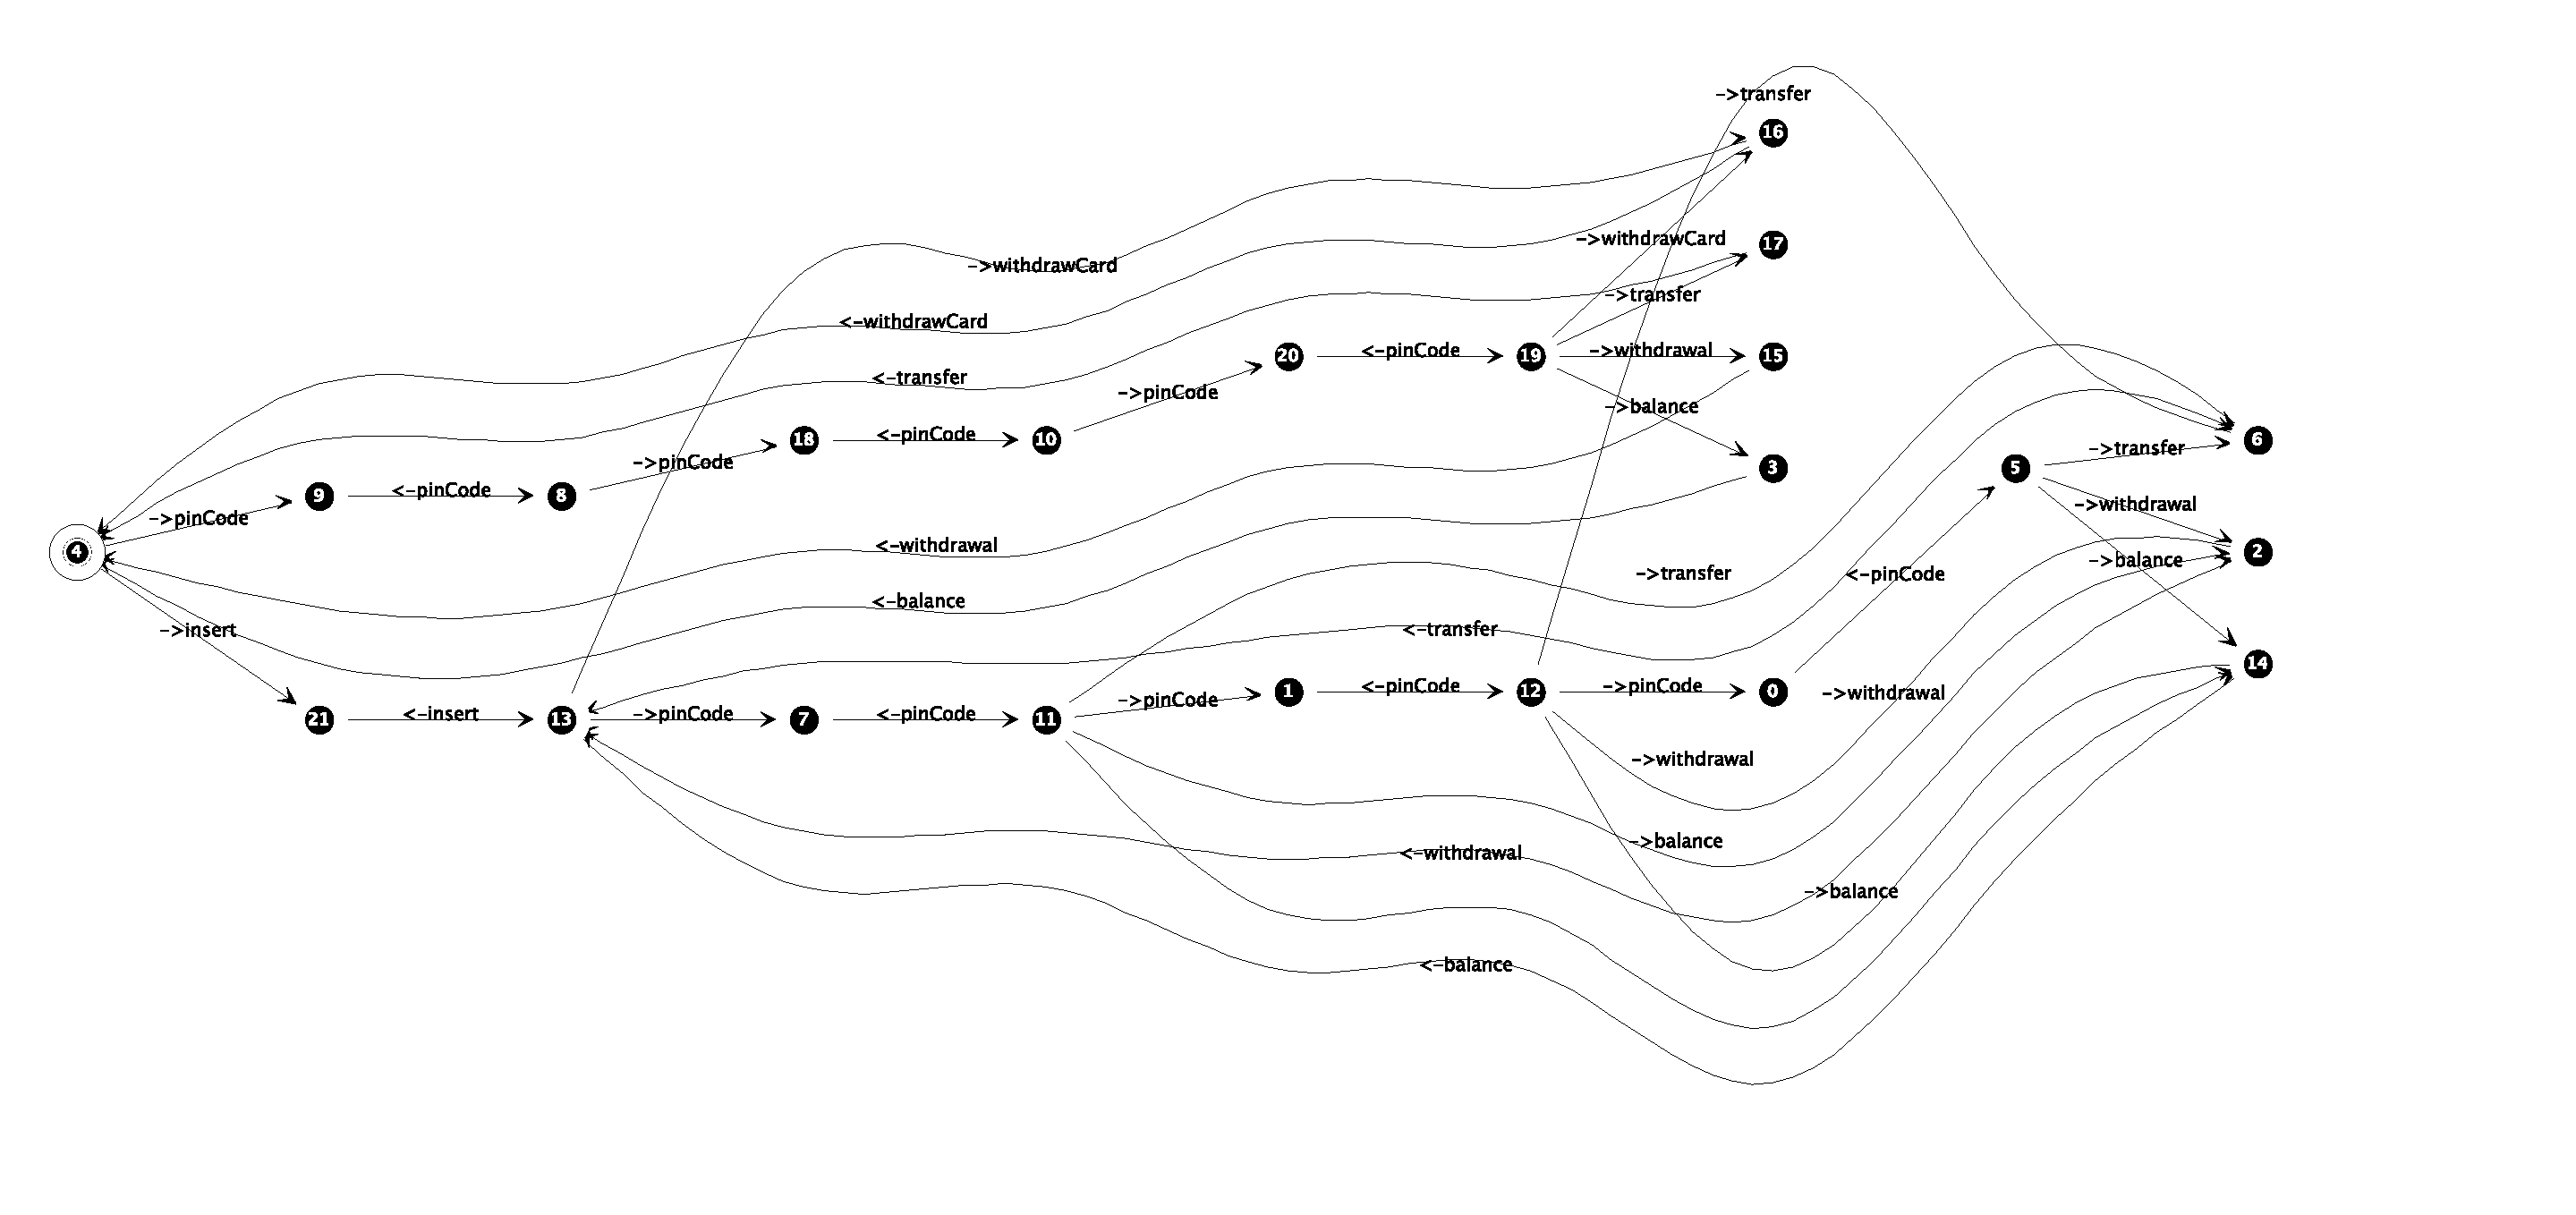
\includegraphics[width=1.2\textwidth]{figures/fig-dab-abstract-min.eps}
%%     \caption{Automate abstrait de l'interface DAB}
%%     \label{fig-auto-dab-abstract}
%% \end{figure}

%% On peut donc construire un observateur pour cette propri\'et\'e
%% d'ind\'ependance.

 
%% \subsection{Test de r\'esilience}

%% \section{Conclusion}

%% D\'efinir testeur. Les testeurs qui nous int\'eressent sont
%% sp\'ecifiques \`a la structure des composants (voir test distribu\'e)

%% D\'efinir observateur (testeur local ?)

%% D\'efinir relations de conformit\'e (cf. relation de sous-typage
%% comportemental)

%% D\'efinir testeur pour la conformit\'e (test tous les ports +
%% comportement du composant)

%% D\'efinir testeur pour l'ind\'ependance des facettes
%% (cf. composition, propri\'et\'e 2 des facettes) = test facettes 1
%% par 1 

%% D\'efinir testeur pour la r\'esilience = test 1 facette correcte et
%% les autres incorrectes

%% Probl\`eme de la compl\'etude des tests ? exhaustivit\'e wrt
%% relation de conformit\'e ?


%% %%          r\'esilience n. f.
        
%% %% D\'efinition (physique) :
%% %% Rapport de l'\'energie restitu\'ee \`a l'\'energie fournie,
%% %% apr\`es un retour rapide ou instantan\'e et complet ou presque \`a
%% %% la forme initiale d'un \'echantillon d\'eform\'e. 

        
%% %% D\'efinition (m\'edecine) :
%% %% R\'esistance d'un mat\'eriau aux chocs r\'ep\'et\'es. S'exprimant
%% %% en Kg par cm$^2$, la r\'esilience est le rapport de l'\'energie
%% %% cin\'etique absorb\'ee n\'ecessaire \`a provoquer la rupture d'un
%% %% 6mat\'eriau, \`a la surface de la section bris\'ee. 

        
%% %% D\'efinition (psychologie) :
%% %% Aptitude \`a faire face avec succ\`es \`a une situation
%% %% repr\'esentant un stress intense en raison de sa nocivit\'e ou du
%% %% risque qu'elle repr\'esente, ainsi qu'\`a se ressaisir, \`a
%% %% s'adapter et \`a r\'eussir \`a vivre et \`a se d\'evelopper
%% %% positivement en d\'epit de ces circonstances d\'efavorables. 

%% %% R\'ESILIENCE, subst. f\'em.
%% %% A. M\'ECAN., PHYS. R\'esistance d'un mat\'eriau au
%% %% choc. Coefficient de r\'esilience. Il ne serait pas normal d'utiliser
%% %% en carrosserie, en aviation, ou dans des pi\`eces de machines, des
%% %% bois qui n'auraient pas une r\'esilience suffisante (CAMPREDON, Bois,
%% %% 1948, p. 459). 
%% %% B. ZOOL. ,,Capacit\'e de reproduction d'une esp\`ece animale
%% %% inemploy\'ee en raison d'une ambiance hostile, mais susceptible d'une
%% %% expansion soudaine si cette ambiance s'am\'eliore. \og (Husson
%% %% 1970). Les Cyprinid\'es ont parmi les Poissons une forte
%% %% r\'esilience en raison du grand nombre d'\oe ufs qu'ils pondent
%% %% (Husson 1970) \fg. 
%% %% C. Au fig., rare. Force morale; qualit\'e de quelqu'un qui ne se
%% %% d\'ecourage pas, ne se laisse pas abattre. \og Dans ce deuil, une fois
%% %% encore, elle \'etonna ses amis par son imm\'ediate r\'esilience
%% %% (MAUROIS, L\'elia, 1952, p. 469 ds QUEM. DDL t. 22)\fg . 
%% %% Prononc.: []. \'Etymol. et Hist. 1906 r\'es\'elience (La Vie au
%% %% grand air, 19 janv., p. 53b ds QUEM. DDL t. 17); 1911 r\'esilience
%% %% (Lar. mens., janv., p. 20). Empr. \`a l'angl. resilience, att. dans
%% %% ce sens d\`es 1824 (NED), sp\'ecialisation de resilience \og fait
%% %% de rebondir\fg (1626, BACON, ibid.), d\'er. de resilient,
%% %% propr. \og rejaillissant, rebondissant \fg (resilient*). REY-GAGNON
%% %% Anglic. 1981. Bbg. DUB. D\'er. 1962, p. 65. 

%% \section{Exp\'erimentation}

%%% Local Variables: 
%%% mode: latex
%%% TeX-master: "these"
%%% TeX-master: "these"
%%% TeX-master: "these"
%%% TeX-master: "these"
%%% TeX-master: "these"
%%% End: 
 
\chapter{Mise en \OE uvre}
\label{cha:methodes--outils}

Nous revenons dans ce chapitre \`a des aspects plus pratiques de la
mise en  \oe uvre des mod\`eles et concepts pr\'esent\'es
pr\'ec\'edemment dans le cadre d'un processus de d\'eveloppement. 
L'objectif de ce chapitre est de d\'ecrire d'une part comment sont produits et
manipul\'es les mod\`eles \textsf{FIDL} d'architecture de
composants et d'autre part comment la g\'en\'eration et
l'ex\'ecution des tests \`a partir des mod\`eles s'ins\`ere dans
le processus de d\'eveloppement. 

\section{Processus de test}

Nous d\'etaillons dans cette section le processus concret de test de
composants \`a partir de mod\`eles \textsf{FIDL}.

\subsection{Plateforme de test}

\`A partir d'une description quelconque d'un mod\`ele FIDL, par
exemple en utilisant la syntaxe \textsf{IDL3} \'etendue
pr\'esent\'ee au chapitre \ref{chap-fidl}, on construit une
repr\'esentation m\'emoire des diff\'erents objets
sp\'ecifi\'es. Ces objets sont r\'epartis en quatre cat\'egories distinctes :
\begin{itemize}
  \item les types de donn\'ees primitifs et construits, y compris les types
    d'\'ev\'enements et les types d'exception ;
  \item les entit\'es arcitecturales, interfaces, composants et
    assemblages ; 
  \item les descriptions de comportements autrement dit les automates
    \textsf{FIDL} ;
  \item les fonctions et pr\'edicats utilis\'es dans les contraintes
  sur les automates \textsf{FIDL}.
\end{itemize}

Les types de donn\'ees, les fonctions et pr\'edicats sont
compil\'es dans le langage d'implantation choisi pour la partie
fonctionnelle du mod\`ele \textsf{FIDL}. En l'\'etat actuel de la
plateforme, ces objets permettent de produire un ensemble de types de
donn\'ees et de fonctions du langage Jaskell qui sont ensuite
compil\'es vers du code-octet \textsf{Java}. 

En fonction du choix de la plateforme technique d'ex\'ecution des
tests, c'est \`a dire du choix du mode de d\'eploiement et
d'implantation des composants, un certain nombre de souches sont
g\'en\'er\'ees \`a partir des interfaces ou extraites de
l'implantation. Dans le cas des composants CCM et POJO, les
projections des interfaces fournies et requises par le composant sont
normalement incluses dans l'ensemble des classes d'implantation et il
n'est donc pas n\'ecessaire de les g\'en\'erer. 

On choisi ensuite la sp\'ecification \`a tester et on d\'efinit le
mode de d\'eploiement du CUT. \`A chaque plateforme technologique
est associ\'e un d\'eployeur sp\'ecifique qui a pour fonction :
\begin{itemize}
  \item de construire un contexte d'ex\'ecution permettant au CUT de
  s'ex\'ecuter normalement. Dans le cas de composants CCM ou de
  composants de type applications Web ou EJB, ce contexte
  d'ex\'ecution est un container du type appropri\'e. Dans le cas de
  composants POJO, ce contexte est simplement un flot d'ex\'ecution
  Java repr\'esentant l'application dont peut faire partie le
  composant ;
\item de r\'ealiser et de maintenir les connexions correspondant \`a
  chaque port du composant. Chaque connexion doit assurer la
  transformation des messages dans la technologie appropri\'ee pour
  le port consid\'er\'e et inversement, ce que l'on nomme
  \emph{marshalling}. \`A noter qu'il n'est pas n\'ecessaire qu'un
  composant donn\'e se limite \`a un mode de connexion. Par exemple,
  un composant servlet peu avoir un port fourni communiquant par
  protocole HTTP et un port requis communiquant par RPC. 
\end{itemize}
On notera que le connecteur doit aussi assurer la transformation des
donn\'ees transport\'ees par les messages depuis/vers les types
manipul\'es par les fonctions et pr\'edicats dans les automates
\textsf{FIDL}.

Une fois le composant \`a tester pr\^et \`a s'ex\'ecuter, on
d\'etermine les param\`etres de la session de test :
\begin{itemize}
  \item l'automate actif pour la session d\'etermine la strat\'egie
    de test pour cette session. Cet automate peut \^etre soit
    l'automate de la sp\'ecification d'un port, soit un automate de la
    sp\'ecification du composant ; 
  \item les param\`etres de contr\^ole de la fonction d'\'evaluation
    : valuation des diff\'erents crit\`eres de s\'election et
    objectif \`a atteindre pour la session ;
  \item les g\'en\'erateurs pour les variables apparaissant dans les
  messages d'entr\'ee du composant peuvent \^etre param\'etr\'es,
  soit avec un enesemble fini de valeurs \`a tester, soit avec une
  fonction de g\'en\'eration. Ce point est un des plus d\'elicats
  car du choix des valeurs peut d\'ependre l'ex\'ecutabilit\'e de
  certains chemins dans l'automate \textsf{FIDL}.
\end{itemize}

La session peut alors d\'emarrer : le contr\^oleur de test
g\'en\'eral met en \oe uvre les algorithmes d\'etaill\'es dans le
chapitre pr\'ec\'edent pour choisir les chemins d'ex\'ecution de la
session de test et v\'erifie que les messages provenent du CUT sont
bien conformes \`a ceux attendus. En cas de besoin, le CUT peut
\^etre reinitialiser et donc red\'eployer.

\subsection{Exemple de mise en \oe uvre}



\section{Mod\`eles et processus de d\'eveloppement}

La premi\`ere \'etape consiste \`a disposer d'un mod\`ele
\textsf{FIDL} de l'application. Ce mod\`ele peut provenir de
diff\'erentes sources sous r\'eserve de disposer d'une extension
sp\'ecifique au langage utilis\'e pour d\'ecrire le mod\`ele
FIDL.  Un mod\`ele FIDL est suppos\'e \^etre exprim\'e sous la
forme d'une instance du m\'eta-mod\`ele FIDL. La transformation \`a
partir d'un autre mod\`ele, par exemple, UML, EdoC, Fractal ou autre,
est une \'etape pr\'ealable. Cette instance peut-\^etre sous
diff\'erentes formes dont les plus courantes sont :
\begin{itemize}
  \item le format \textsf{XMI} qui une repr\'esentation XML d'un
  mod\`ele ou m\'eta-mod\`ele \textsf{UML} ;
\item le format \textsf{IDL3} annot\'e, dont le corps respecte la
  grammaire usuelle des descriptions de composants IDL3 et dont les
  commentaires peuvent contenir des descriptions de comportement sous
  la forme d'expressions \textsf{FIDL}. 
\end{itemize}

Ce mod\`ele constitue l'entr\'ee d'un certain nombre de modules :
\begin{itemize}
  \item le contr\^oleur de mod\`ele qui v\'erifie la coh\'erence
  s\'emantique des mod\`eles, c'est \`a dire les propri\'et\'es
  de compositionnalit\'e d\'efinies au chapitre
  \ref{cha:composition} : ind\'ependance des facettes et respect des
  ports. Le contr\^oleur de mod\`ele v\'erifie aussi la
  validit\'es des relations de sous-typage entre interfaces et entre
  composants ;
\item le g\'en\'erateur de test qui produit des cas de tests
  statiques abstraits \`a partir des descriptions comportementales
  d'un composant et d'objectifs de couverture ;
\item le g\'en\'erateur de testeur qui produit un testeur dynamique,
  c'est \`a dire un programme ex\'ecutable testant dynamiquement
  selon les algorithmes pr\'esent\'es dans le chapitre
  pr\'ec\'edent un ou plusieurs composants ;
\item un d\'eployeur qui, \`a partir d'un mod\`ele et d'une
  implantation dans une ou plusieurs plate-formes sp\'ecifiques est
  capable de lier un testeur et  un composant r\'eel. 
\end{itemize}

\subsection{D\'eploiement \& Ex\'ecution}

Le d\'eploiement d'un composant r\'eel est une op\'eration
d\'ependant du medium de communication et de la structure du
composant lui-m\^eme. Par d\'eploiement, on
entend la construction d'un environnement permettant \`a un testeur
et \`a un composant de communiquer. Le r\^ole du d\'eployeur est
\`a l'ex\'ecution de traduire les messages entre le formalisme
\textsf{FIDL} et le protocole effectif utilis\'e par le composant
test\'e.

Un d\'eployeur est configur\'e d'une part par le mod\`ele
d'ex\'ecution du composant, d'autre part par un mod\`ele de
communication. Le mod\`ele d'ex\'ecution d\'efinit comment est
suppos\'e s'ex\'ecuter le composant r\'eel. Dans le cas le plus
simple, il n'y a rien \`a faire : le composant est d\'ej\`a
d\'eploy\'e par ailleurs et seule la communication doit \^etre
prise en charge. Dans d'autre cas (CCM, EJB, WebApps), un contexte
d'ex\'ecution simul\'e totalement ou partiellement doit \^etre mis
en place. 

Le mod\`ele de communication d\'efinit concr\`etement comment
transformer les messages entre le composant et le testeur. En fonction
de la configuration choisie, le d\'eployeur met en place un canal de
communication par port du composant \`a tester, c'est \`a dire par
port identifi\'e dans le mod\`ele \textsf{FIDL}. Il n'est pas
n\'ecessaire que tous les ports communiquent selon un m\^eme
protocole. Un composant peut par exemple communiquer sous la forme
d'appels de m\'ethodes classiques en  \textsf{Java} et  par ailleurs
sous la forme de flux dans des fichiers selon un mod\`ele
\textsf{UNIX}. Une autre configuration courante est celle d'un
composant Web communiquant avec un client dans un protocole
\textsf{HTTP} et avec un serveur en appels de m\'ethodes. 

Les protocoles pris en charge par le prototype sont :
\begin{itemize}
  \item l'appel de m\'ethode local (dans une m\^eme \textsf{JVM}) ;
  \item l'appel de m\'ethode distant par \textsf{RMI},
    \textsf{XML-RPC} ou \textsf{SOAP} ;
  \item l'\'echanges de donn\'ees dans des formulaires \textsf{HTTP},
    soit directement par g\'en\'eration de requ\^etes/r\'eponses
    HTTP 1.1, soit par construction de requ\^etes/r\'eponses dans un
    contexte de \emph{Servlets}.
\end{itemize}

Les mod\`eles d'ex\'ecution pris en charge sont :
\begin{itemize}
  \item composants \textsf{POJO} ;
  \item composants \textsf{OpenCCM} ;
  \item composants \textsf{J2EE} : \emph{Servlets} et \textsf{EJB}.
\end{itemize}

\subsection{V\'erifications}

L'outil de v\'erification effectue donc un certain nombre de
contr\^oles sur le ou les mod\`eles FIDL qui lui sont fournis. Les
v\'erification syntaxiques et de bonne formation des expressions sont
r\'ealis\'ees \`a la vol\'ee par l'analyseur syntaxique \`a
partir d'un descripteur \textsf{IDL3}. Un mod\`ele \textsf{FIDL} en
m\'emoire est suppos\'e correctement form\'e, au sens de
\ref{def:automate-bien-forme}. 

Dans l'\'etat actuel du prototype, toutes les v\'erifications sont
effectu\'ees sur une version simplifi\'ee du langage des composants
et des interfaces. Ce langage simplifi\'e ignore les contraintes et
distingue uniquement les valeurs litt\'erales et les variables,
d\'enot\'ees par leur type. La premi\`ere \'etape de
v\'erification consiste en la construction des langages des
diff\'erents objets, selon les d\'efinitions du chapitre
\ref{cha:composition} : langages d'interfaces, langages de composants,
langages d'assemblages. 

Les v\'erifications r\'ealis\'ees sont donc :
\begin{itemize}
  \item pour les interfaces dans une relation d'h\'eritage, la
    v\'erification de l'h\'eritage comportemental au sens de
    \ref{sec:heritage-comportemental} ;
  \item pour les composants et assemblages :
    \begin{itemize}
      \item la v\'erification du respect des facettes et r\'eceptacles
        ;
      \item la v\'erification de l'ind\'ependance des facettes et des
        puits (sur les alphabets abstraits) ;
      \item \'eventuellement le respect de l'h\'eritage comportemental
        lorsqu'une relation d'h\'eritage explicite est donn\'ee.
    \end{itemize}
\end{itemize}

La relation contractuelle peut aussi \^etre v\'erifi\'ee
explicitement entre deux composants ou assemblages. 

\subsection{Test}

Les tests \`a partir de mod\`eles \textsf{FIDL} peuvent \^etre
r\'ealis\'es selon deux modalit\'es :
\begin{itemize}
  \item traditionnelle : un certain nombre de cas de
  test sont g\'en\'er\'es, puis ensuite ex\'ecut\'es en tant que
  cas de test \textsf{JUnit} ;
\item dynamique : un testeur implantant l'interface
  \textsf{TestRunner} de \textsf{JUnit} ex\'ecute des tests de
  mani\`ere adaptative en fonction des r\'eponses re\c{c}ues depuis
  l'\textsf{IUT} et selon les strat\'egies d\'efinies dans le
  chapitre \ref{cha:selection-des-cas}.
\end{itemize}

Dans ce second cas de figure, l'int\'egration avec JUnit se fait en
consid\'erant que toute op\'eration de \texttt{reset} signale une
fin de test unitaire r\'eussi qui est donc indiqu\'ee comme tel au
framework \textsf{JUnit}.

\subsection{Couverture de code}

Le test \`a partir d'un mod\`ele \textsf{FIDL} peut \^etre
\'evidemment coupl\'e avec une analyse de la couverture du code du
composant r\'eel lorsque celui-ci est disponible localement. Cette
information est extr\^emement int\'eressante puisqu'elle permet de
savoir quelle fraction du code d\'evelopp\'e est couverte par la
sp\'ecification mod\'elis\'ee ou de mani\`ere \'equivalente quel
partie de la sp\'ecification est r\'eellement ex\'ecutable dans le
code. 

\subsection{Granularit\'e du test}

Le principal int\'er\^et du mod\`ele d'architectures que nous avons
propos\'e est de permettre de tester \`a partir du m\^eme outil et
de fa\c{c}on syst\'ematique les fonctionnalit\'es d'un ensemble de
composants produisant un syst\`eme par assemblage. Selon les choix
fait dans le processus de d\'eveloppement et le degr\'e de
pr\'ecision de la mod\'elisation, les tests pourront \^etre
r\'ealis\'es \`a diff\'erents niveaux. 

Dans le cas le plus simple, seul un sous-syst\`eme complet, par exemple un
cas d'utilisation dans l'exemple de la m\'ethodolgie pr\'esent\'ee
au chapitre \ref{cha:proc-de-devol}, sera mod\'elis\'e de mani\`ere
formelle en utilisant des sp\'ecifications \textsf{FIDL}. \`A partir
de cette mod\`elisation on produira alors un  testeur syst\`eme
dont les connexions seront instanci\'ees avec les protocoles les plus
externes de l'application consid\'er\'ee. 

Dans le cas id\'eal, chaque composant de chaque couche de
l'application sera mod\'elis\'e et sp\'ecifi\'e sous la forme d'un
composant FIDL, l'ensemble \'etant organis\'e sou forme d'assemblage
hi\'erarchique. Les propri\'et\'es que nous avons d\'emontr\'ees
dans les chapitres pr\'ecedents permmettront d'all\'eger l'effort de
test d'int\'egration : la v\'erification du respect des contrats par
les composants garantit par la suite la correction de l'assemblage.

\section{Exemple}



\section{Outillage}

La majeure partie des mod\`eles et algorithmes d\'efinis dans les
chapitres pr\'ec\'edent a \'et\'e implant\'ee sous la forme de
biblioth\`eques et de programme \textsf{Java} destin\'es \`a
s'int\'egrer dans un processus de d\'eveloppement et
d'int\'egration continue. Nous pr\'esentons ici sommairement chacun
de ces composants. 



Strat\'egie g\'en\'erale : pas de plateforme unique (eg. Eclipse)
faisant tout, processus souple et agile, ind\'ependant technologie :
mod\`ele UniX : un ensemble de petits outils qui font chacun une
chose et le font bien. ID : extrapolation du mod\`ele de flux texte
Unix au flux arborescents/graphes (textutils), production de scripts
de transformation/manipulation de mod\`eles (cf. travaux autour de
QVT, transformation de mod\`eles, MDA, MDE, ...)

production de mod\`eles testables : m\'eta-mod\`eles bas\'es sur
une architecture de composants, extractions de mod\`eles \`a partir
d'existant (approche Hood), transformations de mod\`eles existants :
mod\`eles de classes UML avec st\'er\'eotypes, mod\`eles de
composants, mod\`eles AADL, ...format pivot = IDL3/FIDL

partie dynamique : lien entre diff\'erents mod\`eles \`a base de
syst\`emes de transitions d'\'etats finis : mod\`ele FIDL
repr\'esente une approximation pessimiste et v\'erifiable du
comportement r\'eel.  Lien avec IOLTS (LOTOS) et EFSM
(Statecharts). Voir liens avec OCL : description des contraintes. 

liaison avec le code : PSM : couche de projection entre les mod\`eles
de composants et les mod\`eles concrets. rester le + longtemps
possible dans les couches abstraites. 

Mod\`ele de composant
utilis\'e \`a la fois pour v\'erification et pour d\'eploiement :
production de descripteurs automatiques, g\'en\'eration de code
d'interfaces/stubs/squelettes/souches/...

V\'erification existant vs. projection (cf chapitre 1, conclusion) :
ex. Macker, v\'erification de contraintes architecturales \`a partir
des r\`egles de projection : permet d'utiliser le m\^eme formalisme
et les m\^emes jeu de r\`egles pour produire du code et pour
v\'erifier du code existant. 

Int\'egration dans le processus de d\'eveloppement : versionning de
mod\`ele/code g\'en\'er\'e et enrichi. Pb: distinguer les parties
g\'en\'er\'ees des parties \'ecrites, maintenir la coh\'erence
entre les mod\`eles et le code source. Utilisation de balises, diff,
syst\`eme standard de gestion de version, r\'econciliation (merge) :
\'evolution parall\`ele des mod\`eles et du code. 

R\'ef\'erentiel de mod\`eles : modfact, mdr, emfcore. Outil central
pour le d\'eveloppement.

Ex\'ecution des tests : g\'en\'eration de testeurs sp\'ecifiques
au d\'eploiement. Production de connecteurs ad-hoc en fonction de la
plateforme cible : les tests sont g\'en\'eriquement ex\'ecut\'es
et transform\'es \`a la vol\'ee en fonction de la cible. (exemple :
OpenCCM, Java). Connecteurs entre deux techno : Java <-> Http ? Java
<-> OpenCCM, OpenCCM <-> .Net, ....

Couverture / Fiabilit\'e des tests : d\'efinition d'une strat\'egie
adaptative en fonction des risques, possibilit\'e d'atteindre 100\%
dans certains cas, mod\`ele g\'en\'erique de couverture applicable
\`a n'importe quel syst\`eme de transition. 

Strat\'egie de test d'architecture : diminuer l'int\'er\^et du test
d'int\'egration en accroissant la qualit\'e et la fiabilit\'e des
tests unitaires (test de conformit\'e, test d'ind\'ependance, test
de r\'esilience). Utiliser diff\'erents niveaux de description
d'architecture : strat\'egie risque/rentabilit\'e, optimiser le
nombre de tests et les temps d'ex\'ecution sur les \'el\'ements les
plus strat\'egiques (voir en fonction de la complexit\'e des
automates, mesure du nombre cyclomatique : choisir d'abord les
sp\'ecifications les plus complexes ou leur allouer plus de temps
d'ex\'ecution que les autres voir mesure de la fiabilit\'e en
fonction du temps CPU de Musa\cite{musa-theory-sr}

Objectif g\'en\'eral : accroissement  de la fiabilit\'e => mesure
\`a partir des anomalies remont\'ees en TMA (hors demande
d'\'evolutions) : n\'ecessite de faire une \'etude sur l'impact du
test architectural sur la fiabilit\'e g\'en\'erale : analyse des
erreurs d\'etect\'ees par le test avant recette et des erreurs
r\'ev\'el\'ees en recette (historique des erreurs :
traceabilit\'e, cas de test).

\section{M\'ethodes \& Outils pour les architectures de composants}

\section{Pratique du test de composants \textsf{FIDL}}

\subsection{La plateforme de test \textsf{FIDL}}

Analyse de mod\`ele FIDL : v\'erifications  de base (syntaxe,
s\'emantique : projections sur alphabets abstraits, ind\'ependance,
....)

G\'en\'eration de cas de test


%%% Local Variables: 
%%% mode: latex
%%% TeX-master: "these"
%%% TeX-master: "these"
%%% End: 
  
\chapter*{Conclusion}
%\label{cha:conclusion}
%%% Local Variables: 
%%% mode: latex
%%% TeX-master: "these"
%%% End: 

\bibliographystyle{acm}
\bibliography{bibsingle}

%%% Local Variables: 
%%% mode: latex
%%% TeX-master: "these"
%%% End: 

%% \appendix
%% \chapter{Exemple de codes}
%% \label{cha:exemple-de-codes}
%% %\lstset{basicstyle=\footnotesize\sffamily,frame=none}

\section{Exemple d'applications de gestion de commandes}

\begin{lstlisting}
module Commande {

   exception CommandeInvalide {};
   exception PaiementInvalide {};
   exception CarteInvalide {};
   exception MontantIncorrect {};

   struct article {
      long ref; 
      long prix;
      short qte;
   };
 
    struct commande {
      long id;
      long montant;
      sequence<article> articles;
   };
   
   struct paiementBA {
      long ref;
      long montant;
   };

   struct paiementCB {
      string numeroCB;
      string expiration;
      string cle;
      long montant;
   };

  eventtype CommandeEvent { public commande com; };

  interface Commande {
      commande nouvelleCommande();
      void ajouterArticle(in commande c,in article a);
      boolean validerCommande(in commande c);
      void annulerCommande(in commande c);

      /*** FIDL
        (com in nouvelleCommande(:com) ajouterArticle(_,_)* 
          ((->validerCommande(com) <-validerCommande(:false))* annulerCommande(com) + 
            ->validerCommande(com) <-validerCommande(:true)))*
       */
   };

   interface Paiement {
      void ajouterPaiementBA(in commande com,in paiementBA ba) 
         raises (PaiementInvalide, CommandeInvalide);
      void ajouterPaiementCB(in commande com,in paiementCB cb) 
         raises (PaiementInvalide, CommandeInvalide, CarteInvalide);
      boolean validerPaiement(in commande com) 
         raises (CommandeInvalide, MontantIncorrect);
      void annulerPaiement(in commande com);

      /*** FIDL
          ((->ajouterPaiementBA(_,_) (<-ajouterPaiementBA() + 
                                  <-ajouterPaiementBA<PaiementInvalide> + 
                                  <-ajouterPaiementBA<CommandeInvalide>) 
           ->ajouterPaiementCB(_,_) (<-ajouterPaiementCB() + 
                                  <-ajouterPaiementCB<PaiementInvalide> + 
                                  <-ajouterPaiementCB<CarteInvalide> + 
                                  <-ajouterPaiementCB<CommandeInvalide>))*
            (->validerPaiement(_) (<-validerPaiement<CommandeInvalide> + 
                                 <-validerPaiement<MontantIncorrect>))*
             (annulerPaiement(_)+
              validerPaiement(_:_)))*                                 
       */
    };

    component Store {
        provides Commande com;
        provides Paiement pai;
        publishes CommandeEvent ev;
     
        /*** FIDL
            (cm in com.nouvelleCommande(:cm) pai.validerPaiement(cm:true) 
               com.validerCommande(cm:true) ev[cm])*
         @@ 
            (cm in com.nouvelleCommande(:cm) pai->validerPaiement(cm) 
               pai<-validerPaiement<MontantIncorrect> com.validerCommande(cm:false))*
         @@ 
            com.validerCommande(_:false)*
         @@
            (pai->validerPaiement(_) pai<-validerPaiement<CommandeInvalide>)*
         */
    };         
};

module Paiement {
     
    interface PaiementCB {
         boolean validerNumero(in string numero);
         boolean carteEnOpposition(in string numero);

        /*** FIDL 
          (validerNumero(_:_) + carteEnOpposition(_:_))*
         */
    };
    
    interface PaiementBA {
         boolean validerBA(in long ref);

        /*** FIDL
          (validerBA(_:_))*
         */
    };

    interface EtatReglement {
        boolean paiementOK(in ::Commande::commande com);

        /*** FIDL
           paiementOK(_:_)*
         */
         
    };

    component Reglement {
        provides Commande::Paiement pai;
        provides EtatReglement etat;
        uses     PaiementCB cb;
        uses     PaiementBA ba;

        /*** FIDL 
           (cb,cm in pai->ajouterPaiementCB(cm,cb) cb.validerNumero(cb.numeroCB:true) 
                                             cb.carteEnOpposition(cb.numeroCB:false)
                                             pai<-ajouterPaiementCB())*
          @@
           (cb in pai->ajouterPaiementCB(_,cb)
             cb.validerNumero(cb.numeroCB:false) 
             pai<-ajouterPaiementCB<Commande::CarteInvalide>)*
          @@
           (cb in pai->ajouterPaiementCB(_,cb) 
              cb.carteEnOpposition(cb.numeroCB:true) 
              pai<-ajouterPaiementCB<Commande::CarteInvalide>)*
          @@ 
           (ba in pai->ajouterPaiementBA(_,ba) 
              ba.validerBA(ba.ref : true) pai<-ajouterPaiementBA())*
          @@ 
           (ba in pai->ajouterPaiementBA(_,ba) 
              ba.validerBA(ba.ref : false) 
              pai<-ajouterPaiementBA<Commande::PaiementInvalide>)*
          @@
           (cm in pai.validerPaiement(cm:true) etat.paiementOK(cm:true))*
          @@
            etat.paiementOK(_:false)*
         */
     };    

     component Order {
         provides Commande::Commande com;
         uses EtatReglement reg;
         publishes Commande::CommandeEvent ev;

         /*** FIDL
            (cm in com->validerCommande(cm) 
               (reg.paiementOK(cm:true) com<-validerCommande(true) ev[cm] +
                reg.paiementOK(cm:false) com<-validerCommande(false)))*
          */
            
     };
};
\end{lstlisting}

%%% Local Variables: 
%%% mode: latex
%%% TeX-master: "these"
%%% End: 

%% \chapter{Grammaire FIDL}
%% \label{cha:grammaire-fidl}
%% %\section{FIDL}
\label{annexe-grammaire-fidl}

\begin{tabbing}
aaaaaaaaaaaaaaaaaaaaaaaa\=aaa\=aaa\=and \=aaa\=aaaaaaaaaaaaaaaaaaaaaa\=aaa\=aaaaaaaaaaaaaaaaaa\=\kill
\emph{specification-fidl}\>\twocol=\> \texttt{FIDL} \emph{comportement}\\
\>$\mid$\>\texttt{header} \emph{function\_headers} \texttt{FIDL} \emph{comportement} 
\texttt{body} \emph{function\_bodies}\\

\emph{comportement}\>\twocol=\>  \emph{specification-facettes} \emph{expression-comportement} \\
    \>$\mid$\> \emph{expression-comportement} \\

\emph{specification-facettes}\>\twocol=\>  \texttt{facets} \emph{liste-facettes} \texttt{;}\\

\emph{liste-facettes}\>\twocol=\>  \emph{liste-facettes} \texttt{,} \emph{facette} \\
    \>$\mid$\> \emph{facette} \\

\emph{facette}\>\twocol=\> \texttt{multiple}\emph{port\_name} \\
    \>$\mid$\> \texttt{single} \emph{port\_name} \\
    \>$\mid$\> \texttt{unique} \emph{port\_name} \\

\emph{expression-comportement}\>\twocol=\>  \emph{expression-comportement} \verb+@@+ \emph{expression-elementaire} \\
    \>$\mid$\> \emph{expression-elementaire}\\

\emph{expression-elementaire}\>\twocol=\>  \emph{contrainte} \texttt{in} \emph{expression-base} \\
    \>$\mid$\> \emph{expression-base}\\

\emph{contrainte}\>\twocol=\> \emph{contrainte} \texttt{;} \emph{decl-variable} \\
    \>$\mid$\> \emph{decl-variable}\\

\emph{decl-variable}\>\twocol=\>\emph{variable\_name} \texttt{:} \emph{expr-contrainte} \\
    \>$\mid$\> \emph{variable\_name} \texttt{::} \emph{type\_name} \\

\emph{expression-base}\>\twocol=\> \emph{expression-base} \verb+||+ \emph{expression-par} \\
    \>$\mid$\> \emph{expression-par} \\

\emph{expression-par}\>\twocol=\>  \emph{expression-par} \verb|+| \emph{expression-alt} \\
    \>$\mid$\> \emph{expression-alt}\\

\emph{expression-alt}\>\twocol=\>  \emph{expression-alt} \emph{expression-star} \\
    \>$\mid$\> \emph{expression-star} \\

\emph{expression-star}\>\twocol=\>  \emph{expression-atom} \texttt{*} \\
    \>$\mid$\> \emph{expression-atom} \\


\emph{expression-atom}\>\twocol=\> \emph{message} \\ 
    \>$\mid$\>\texttt{(} \emph{expression-elementaire} \texttt{)}\\

\emph{message}\>\twocol=\>\emph{message\_complet} $\mid$
\emph{message\_simplifie}\\

\emph{message\_complet}\>\twocol=\> \emph{arrow} \emph{method\_name}
\texttt{(} \emph{parametres-message} \texttt{)}  \\
    \>$\mid$\> \emph{port\_name} \emph{arrow} \emph{method\_name} \texttt{(} \emph{parametres-message} \texttt{)}  \\  
    \>$\mid$\> \emph{port\_name}\texttt{[} \emph{parametres-event} \texttt{]}  \\
    \>$\mid$\> \texttt{<-}\emph{method\_name} \texttt{<} \emph{exception} \texttt{>}\\
    \>$\mid$\> \emph{port\_name} \texttt{<-} \emph{method\_name}
    \texttt{<} \emph{exception} \texttt{>}\\

\emph{message\_simplifie}\>\twocol=\> \emph{method\_name} \texttt{(} \emph{parametres-message} \texttt{)}  \\
    \>$\mid$\> \emph{port\_name} \texttt{.} \emph{method\_name} \texttt{(} \emph{parametres-message} \texttt{)}  \\
    \>$\mid$\> \emph{port\_name} \texttt{.} \emph{method\_name}
    \texttt{<} \emph{exception} \texttt{>}\\

    \>$\mid$\> \texttt{void}\\ 

%% \emph{message\_type}\>\twocol=\>\emph{identifiant} \emph{kind}\\
%% \>$\mid$\>\emph{arrow} \\
%% \>$\mid$\>$\varepsilon$ \\

%% \emph{exception\_message\_type}\>\twocol=\>\emph{identifiant} \texttt{.}\\
%% \>$\mid$\>\texttt{<-} \\
%% \>$\mid$\>\emph{identifiant} \texttt{<-} \\
%% \>$\mid$\>$\varepsilon$ \\


\emph{parametres-event}\>\twocol=\>\emph{liste-expr-message}\\
    \>$\mid$\> $\varepsilon$\\

\emph{parametres-message}\>\twocol=\>  \emph{liste-expr-message} \\
    \>$\mid$\> \texttt{:} \emph{expr-message} \\
    \>$\mid$\> \emph{liste-expr-message} \texttt{:} \emph{expr-message} \\
    \>$\mid$\> $\varepsilon$\\

\emph{liste-expr-message}\>\twocol=\>  \emph{liste-expr-message} \texttt{,} \emph{expr-message}\\
    \>$\mid$\> \emph{expr-message} \\

\emph{expr-message}\>\twocol=\> \emph{literal} \\
    \>$\mid$\> \emph{variable\_name}\\
    \>$\mid$\> \verb+_+\\

\emph{exception}\>\twocol=\> \emph{exception\_name} \texttt{[} \emph{liste-expr-message} \texttt{]}\\
    \>$\mid$\>  \emph{exception\_name}\\

\emph{arrow}\>\twocol=\>  \verb+->+ \\
\>$\mid$\> \verb+<-+ \\

\emph{expr-contrainte}\>\twocol=\> \emph{variable\_name} \emph{operator} \emph{expr-fonctionnelle}\\

\emph{expr-fonctionnelle}\>\twocol=\> \emph{variable\_name}  \\
    \>$\mid$\> \emph{literal}  \\
    \>$\mid$\> \emph{function\_name} \texttt{(} \emph{liste-parametres} \texttt{)} \\
    \>$\mid$\> \emph{function\_name} \texttt{(} \texttt{)} \\
    \>$\mid$\> \emph{expr-fonctionnelle} \emph{bin-op}
    \emph{expr-fonctionnelle}\\
    \>$\mid$\> \emph{un-op}  \emph{expr-fonctionnelle}\\
    \>$\mid$\> \texttt{(} \emph{expr-fonctionnelle} \texttt{)} \\

\emph{liste-parametres}\>\twocol=\>\emph{liste-parametres}\texttt{,}
    \emph{parametre-fonction}\\
    \>$\mid$\> \emph{parametre-fonction}\\

\emph{parametre-fonction}\>\twocol=\>\emph{expr-fonctionnelle} \\
    \>$\mid$\> \texttt{Trace}\\
    \>$\mid$\> \emph{message\_complet}\\


\emph{bin-op}\>\twocol=\>\verb+<+ $\mid$ \verb+==+ $\mid$ \verb+>+
$\mid$ \verb+<=+ $\mid$ \verb+>=+ $\mid$ \verb+&&+ $\mid$ \verb+||+
$\mid$ \verb+^^+ $\mid$  \verb+!=+ $\mid$ \verb:+: $\mid$  \verb:-: $\mid$  \verb:*: $\mid$
    \verb:/: $\mid$  \verb:%: \\

\emph{un-op}\>\twocol=\>\texttt{!}\\

\emph{identifiant}\>\twocol=\>  [\texttt{a}-\texttt{z}
\texttt{A}-\texttt{Z}] [ \texttt{a}-\texttt{z} \texttt{A}-\texttt{Z} \texttt{0}-\texttt{9}
\texttt{\_} ]$^*$ \\

\emph{operator}  \>\twocol=\>  \verb+<+ $\mid$ \verb+=+ $\mid$ \verb+>+ $\mid$ \verb+<=+ $\mid$ \verb+>=+ $\mid$ \verb+!=+ \\ %$
%% \emph{operator}  \>\twocol=\> \emph{symbol} $\mid$ \emph{symbol} \emph{symbol} \\ 


%% \emph{symbol}   \>\twocol=\>  \verb+!+ $\mid$ \verb+#+ $\mid$ \verb+%+ $\mid$ \verb+*+ $\mid$ \verb\textdegree{}+\textdegree{} $\mid$ \verb+/+ $\mid$ \verb+<+ $\mid$ \verb+=+ $\mid$ \verb+>+ $\mid$ \verb+?+ $\mid$ \verb+^+ $\mid$ \verb+-+ $\mid$ \verb+~+
%% \\ %$

\emph{literal}\>\twocol=\>  \emph{integer-literal} \\
    \>$\mid$\> \emph{string-literal}  \\
    \>$\mid$\> \emph{character-literal} \\ 
    \>$\mid$\> \emph{floating-pt-literal} \\ 
    \>$\mid$\> \verb+{+ \emph{literal-list} \verb+}+ $\mid$ \verb:{}:\\

\emph{literal-list}\>\twocol=\> \emph{literal-list} \texttt{,} \emph{literal}\\ 
    \>$\mid$\> \emph{literal}\\

\emph{integer-literal}\>\twocol=\> \texttt{0} [\texttt{oO}] [\texttt{0}-\texttt{7}]$^+$ \\
    \>$\mid$\>  \texttt{0} [\texttt{xX}] [\texttt{0}-\texttt{9} \texttt{a}-\texttt{f} \texttt{A}-\texttt{F}]$^+$ \\ 
    \>$\mid$\>  [\texttt{0}-\texttt{9}]$^+$ \\ 

\emph{floating-pt-literal}\>\twocol=\>  [\texttt{0}-\texttt{9}]$^*$ \texttt{.}[\texttt{0}-\texttt{9}]$^+$
\emph{exponent-part} \\
\emph{exponent-part}\>\twocol=\>
[\texttt{e}\texttt{E}] [\texttt{0}-\texttt{9}] \\
    \>$\mid$\>[\texttt{e}\texttt{E}] [\texttt{+}\texttt{-}] [\texttt{0}-\texttt{9}] \\
\>$\mid$\>$\varepsilon$ \\ 

\emph{scoped\_name}\>\twocol=\>\verb+::+ \emph{colon\_name}\\
 \>$\mid$\>\emph{colon\_name}\\

\emph{colon\_name}\>\twocol=\>\emph{colon\_name} \verb+::+ \emph{identifiant}\\
 \>$\mid$\>\emph{identifiant}\\


\emph{function\_headers}\>\twocol=\>\emph{function\_headers}
\texttt{;} \emph{function\_header}  \\
\>$\mid$\>\emph{function\_header}  \\

\emph{function\_header}\>\twocol=\>\emph{function\_name} \texttt{:} \emph{in\_types}
\texttt{$\rightarrow$} \emph{elementary\_type}\\

\>$\mid$\>\emph{function\_name} \texttt{:} \texttt{$\rightarrow$} \emph{elementary\_type}\\

\emph{in\_types}\>\twocol=\>\emph{in\_types} \texttt{,} \emph{in\_type}\\
\>$\mid$\>\emph{in\_type}\\

\emph{elementary\_type}\>\twocol=\> \texttt{long} $\mid$ \dots\\

\emph{in\_type}\>\twocol=\>\emph{elementary\_type} $\mid$
\texttt{Trace} $\mid$ \texttt{Message}\\

\emph{port\_name}\>\twocol=\>\emph{identifiant}\\

\emph{variable\_name}\>\twocol=\>\emph{identifiant}\\

\emph{method\_name}\>\twocol=\>\emph{identifiant}\\

\emph{function\_name}\>\twocol=\>\emph{identifiant}\\

\emph{exception\_name}\>\twocol=\>\emph{scoped\_name}\\

\emph{type\_name}\>\twocol=\>\emph{scoped\_name}\\

\emph{function\_bodies}\>\twocol=\> \emph{selon langage choisi}\\
\end{tabbing}


%%% Local Variables: 
%%% mode: latex
%%% TeX-master: "these"
%%% TeX-master: "these"
%%% TeX-master: "these"
%%% TeX-master: "these"
%%% TeX-master: "these"
%%% TeX-master: "these"
%%% TeX-master: "~/recherche/text/these"
%%% TeX-master: "these"
%%% End: 

%% \chapter{Jaskell}
%% \label{cha:jaskell}
%% %
Nous pr\'esentons dans cette section la syntaxe et la s\'emantique du
langage utilis\'e --- par d\'efaut --- pour la d\'efinition de fonctions
dans les sp\'ecifications \textsf{FIDL}. Ce langage, d\'enomm\'e \textsf{Jaskell}
est une version simplifi\'ee du langage \textsf{Haskell98}, un langage
fonctionnel \`a \'evaluation paresseuse issu de \textsf{ML}. 

La premi\`ere partie explicite les raisons qui nous ont pouss\'e \`a choisir
un tel langage pour l'int\'egrer dans les sp\'ecifications \textsf{FIDL},
la seconde d\'etaille la syntaxe du langage et ses liens avec les
structures \textsf{IDL3} et \textsf{FIDL} et la troisi\`eme en pr\'ecise
la s\'emantique eu \'egard \`a celle des ensembles de traces. 

\subsection{Motivation}

\textsf{Jaskell} est n\'e du besoin d'exprimer des relations entre les
contenus des messages pr\'esents dans les sp\'ecifications FIDL et de
construire ce m\^eme contenu, afin d'obtenir une sp\'ecification la plus
d\'etaill\'ee possible des interactions d'un composant avec son
environnement. Ce langage devait nous permettre, entre autre choses, de :
\begin{itemize}
  \item exprimer des op\'erations arithm\'etiques et math\'ematiques
  usuelles sur diff\'erents types de nombres, entiers et flottants ; 
\item manipuler des structures de donn\'ees standard telle que les
  listes ou les structures ;
\item fournir un niveau de langage suffisamment abstrait pour \'eviter
  d'emp\^etrer l'utilisateur dans des d\'etails d'implantation.
\end{itemize}

Plut\^ot que de d\'efinir un langage propre, nous avons choisi
d'adopter un langage fonctionnel existant, moyennant quelques
adaptations et une substantielle r\'eduction de la puissance du
langage, en l'occurence \textsf{Haskell}. Nous avons en effet \'etait
int\'eress\'e par une caract\'eristique fondamentale de ce langage,
l'\emph{\'evaluation paresseuse} des expressions, qui pr\'esente la particularit\'e
de permettre l'\'ecriture et l'\'evaluation de structures ou de
comportements potentiellement infinis, ainsi que par certains aspects
mineurs de la syntaxe tels que les listes par compr\'ehension ou le
filtrage des param\`etres par motifs --- \emph{pattern-matching}. 

Notre principal argument est que cette expressivit\'e fournie par le
langage doit permettre de d\'efinir des fonctions de haut-niveau de
mani\`ere simple et essentiellement abstraite, un aspect essentiel pour
faciliter l'adoption d'un syst\`eme de sp\'ecification formel. On trouvera
dans \cite{finfunc} un expos\'e saisissant sur les potentialit\'es d'un
langage comme \textsf{Haskell}.

\subsubsection{Aper\c{c}u}

Le lecteur familier d'\textsf{Haskell98} ou ayant lu les
sp\'ecifications du langage dans \cite{h98report} souhaitera peut-\^etre
savoir quelles sont les \'el\'ements de ce langage que l'on ne retrouve
pas dans \textsf{Jaskell}. En voici donc une liste non exhaustive :
\begin{itemize}
  \item le syst\`eme de type complexe a disparu, les types manipul\'es par
  \textsf{Jaskell} \'etant les types d\'efinis par le langage \textsf{IDL}
  ;
\item les espaces de nommage sont aussi fournis par les constructions
  de l'\textsf{IDL3}, ce qui implique d'ailleurs l'existence d'espace
  de nommage hi\'erarchique. Les notions d'importation et d'exportation
  du syst\`eme de \emph{modules} ont aussi disparu ;
\item la notion de \emph{monade} n'est pas utilis\'ee car le langage est
  libre de tout effet de bord ;
\item le filtrage de motif a \'et\'e simplifi\'e par suppression des motifs
  de successeur --- \texttt{n + k} ---, des motifs \texttt{\@} et des
  motifs irr\'efutables.
\end{itemize}

\subsection{Syst\`eme de types}

Chaque expression du langage \textsf{Jaskell} re\c{c}oit un type qui
peut \^etre soit explicitement d\'eclar\'e --- par exemple dans la
section \texttt{headers} --- d'une d\'eclaration \textsf{FIDL}, soit
inf\'er\'e lors de la phase de v\'erification des types. Nous
donnons ici une d\'efinition des types utilis\'es dans
\textsf{Jaskell} ainsi que de la relation de sous-typage ---
not\'ee $\sqsubseteq$ --- utilis\'ee pour la surcharge des
fonctions. 

\begin{definition}[Expression de types]
Une \emph{expression de type} ou un \emph{type} est construit selon les r\`egles
suivantes :
\begin{itemize}
  \item \textbf{Primitives.} $\mathtt{Bool},\mathtt{Char},\mathtt{Int},\mathtt{Long},\mathtt{Float},\mathtt{Double},\mathtt{String}$ sont des types ;
\item \textbf{Variables.} \'etant donn\'e un ensemble d\'enombrable
  de noms de variables $TV$, $x$ est un type, pour tout $x$ dans $TV$
  ;
\item \textbf{Listes.} pour tout type $T$, $[T]$ est un type ;
\item \textbf{Tuples.} pour tout ensemble de type $T_1,T_2, \dots,
  T_n$, $(T_1,T_2,\dots,T_n)$ est un type ;
\item \textbf{Structures.} pour tout ensemble de type $T_1,T_2, \dots,
  T_n$ et tout ensemble de noms $n_1,n_2,\dots,n_n$ tel que $\forall
  i,j, n_i\neq n_j$, $\{n_1 : T_1,n_2 :
  T_2,\dots,n_n : T_n\}$ est un type ;
\item \textbf{Fonctions.} pour tous types $T_1,T_2$, $T_1 \rightarrow
  T_2$ est un type.
\end{itemize}
\end{definition}

\begin{definition}[Sous-typage]
\'Etant donn\'e deux types $T_1$ et $T_2$, on d\'efinit
inductivement la relation de \emph{sous-typage} entre les deux types,
not\'ee $T_1\sqsubseteq T_2$ par les r\`egles suivantes :
\begin{itemize}
  \item si $T_1 = T_2$ alors  $T_1 \sqsubseteq T_2$ ;
  \item si $T_2 \in TV$ alors $T_1 \sqsubseteq T_2$ ;
  \item si $T_1 = [T_1'], T_2=[T-2'], T_1' \sqsubseteq T_2'$ alors $T_1
  \sqsubseteq T_2$;
\item si $T_1 = (t_1,t_2,\dots,t_n), T_2=(q_1,q_2,\dots,q_n),
  \forall i, 1\leq i \leq n, t_i\sqsubseteq q_i$ alors  $T_1
  \sqsubseteq T_2$ ;
\item si $T_1 = \{n_1:t_1,n_2:t_2,\dots,n_n:t_n\}, T_2=\{m_1:q_1,m_2:q_2,\dots,m_n:q_n\},
  \forall i, 1\leq i \leq n, t_i\sqsubseteq q_i$ alors  $T_1
  \sqsubseteq T_2$ ;
\item si $T_1 = t_1 \rightarrow t_2, T_2 = q_1 \rightarrow q_2, t_1
  \sqsubseteq q_1, q_2 \sqsubseteq t_2$ alors $T_1
  \sqsubseteq T_2$ ;
\end{itemize}
De plus, il existe une relation de sous-typage entre les types
primitifs d\'efinis ci-dessus :
$$
\mathtt{Char}\sqsubseteq\mathtt{Int}\sqsubseteq\mathtt{Long}\sqsubseteq\mathtt{Float}\sqsubseteq\mathtt{Double}
$$
\end{definition}

\begin{definition}[Inf\'erence de type]

\end{definition}

\newlength{\oldwidth}
\newenvironment{mytab}{\setlength{\oldwidth}{\linewidth}
  \setlength{\linewidth}{.75\linewidth}\begin{tabbing}}{\end{tabbing}\setlength{\linewidth}{\oldwidth}}

\openout15=jaskellcore-to-java.aux

\def\rulelabel#1{\immediate\write1{\string\newlabel{#1}{{r\therulescount}{\the\count0}}}}
\def\ruleref#1{[\ref{#1}]}

\lstset{language=Java}


\section{Jaskell-Core}

Le langage Jaskell-Core est un langage minimal pr\'eservant la
s\'emantique des constructions de Jaskell tout en enlevant le sucre
syntaxique et en ajoutant des informations de typage. Nous pr\'esentons
ici la syntaxe de ce langage. 

\newcounter{rulescount}
\setcounter{rulescount}{1}
\newcommand{\incrules}{\hfill[r\therulescount]\addtocounter{rulescount}{1}}

\begin{mytab}
\emph{jaskell-part} \= \twocol= \=aaaaaaaaaaaaaaaaaaaaaaaaaaaaaaaaaaaaaaaaaaaaaaaaaa\=\kill
\emph{jaskell} \>\twocol=\> [ \emph{module-decl} ] [ \emph{decl} \texttt{=} \emph{exp} ]$^*$ \rulelabel{prog}\`{\i}ncrules \\
\emph{module-decl}\>\twocol=\> \texttt{module} \emph{qualified-name}
\rulelabel{module}\`{\i}ncrules \\ 
\emph{decl}\>\twocol=\> \emph{identifier} \texttt{\twocol}
\emph{type} \rulelabel{topdecl} \`{\i}ncrules \\
\emph{type} \>\twocol=\> \emph{simple-type} \rulelabel{type} \`{\i}ncrules
 \\
\> $\mid$ \> \emph{type} \texttt{->} \emph{simple-type} \rulelabel{arrowtype}  \`{\i}ncrules
 \\
\emph{simple-type} \>\twocol=\> \emph{qualified-name} [ \emph{type} ]$^*$  \rulelabel{namedtype} \`{\i}ncrules \\
\> $\mid$ \>  \emph{primitive-type}  \rulelabel{primtype} \`{\i}ncrules \\
\> $\mid$ \> \texttt{[} \emph{type} \texttt{]}  \rulelabel{listtype} \`{\i}ncrules \\
\emph{primitive-type} \>\twocol=\> \texttt{Int} $\mid$ \texttt{Float}
$\mid$ \texttt{Double} $\mid$ \texttt{Bool} $\mid$ \texttt{Char} $\mid$ \texttt{String}\\
\end{mytab}

Un source Jaskell est compos\'e d'une succession de d\'efinitions. Ces
d\'efinitions peuvent \'eventuellement \^etre mutuellement r\'ecursives. 

Toutes les d\'efinitions sont compos\'ees d'un identifiant, d'un type
valide attach\'e \`a cet identifiant et d'une expression en 
partie droite \rem{La v\'erification de type ayant d\'ej\`a normalement \'et\'e
  effectu\'ee, le type d'un identifiant sera suppos\'e consistant avec sa
  d\'efinition.}. Les types valides sont construits \`a partir de types 
simples par application de \texttt{->} et \texttt{[]}. Les types
aggr\'egats sont d\'efinis par un nom --- qualifi\'e --- de type et une
liste de types des composants. \rem{Il conviendrait de d\'efinir une
  projection des constructions de types IDL vers Jaskell.}

\begin{mytab}
\emph{binding} \= \twocol= \=aaa\=aaa\=aaa\=aaaaaaaaaaaaaaaaaaaaaaaaaaaaaaaaa\=\kill
\emph{binding} \>\twocol=\> \emph{identifier} 
\texttt{\twocol} \emph{type} \`\`{\i}ncrules \\
\emph{exp} \>\twocol=\>  \texttt{case} \emph{exp} \texttt{of}
\emph{binding} \texttt{\{}
\emph{alts} \texttt{\}}  \rulelabel{case} \`{\i}ncrules \\
\> $\mid$ \> \emph{exp}  \emph{base-exp}  \rulelabel{application} \`{\i}ncrules \\
\> $\mid$ \> $\lambda$ \emph{binding} [ \emph{binding} ]$^*$
\texttt{->} \emph{exp}   \rulelabel{abstraction} \`{\i}ncrules \\
\> $\mid$ \>  \`{\i}ncrules \\
\end{mytab}

Une expression est soit :
\begin{itemize}
  \item une alternative introduite par \texttt{case} ;
  \item une application ;
  \item une abstraction.
\end{itemize}
L'abstraction a pour effet de lier les variables identifi\'ees dans
l'expression en partie droite. L'identifiant apparaissant apr\`es
\texttt{of} dans l'expression de branchement a pour effet de lier la
variable dans toutes les alternatives de l'expression. \rem{Cette
  construction est introduite pour tenir compte des @-patterns.}

\begin{mytab}
\emph{jaskell-part} \= \twocol= \=aaa\=aaa\=aaa\=aaaaaaaaaaaaaaaaaaaaaaaaaaaaaaaaa\=\kill
\emph{alts} \>\twocol=\>  \emph{alt}  \texttt{;} \emph{alts} \`{\i}ncrules \\
\> $\mid$ \> \emph{default-alt}\`{\i}ncrules \\
\emph{alt} \>\twocol=\> \emph{pat} \texttt{->} \emph{exp} \`{\i}ncrules \\
\emph{pat}  \>\twocol=\> \emph{litteral} \`{\i}ncrules \\
\> $\mid$ \> \emph{binding} \`{\i}ncrules \\
\> $\mid$ \> \emph{qualified-name} [ \emph{pat}  ]$^*$ \`{\i}ncrules \\
\> $\mid$ \> \texttt{(:)} \emph{pat} \emph{pat} \`{\i}ncrules \\
\> $\mid$ \> \texttt{[]} \`{\i}ncrules \\
\emph{default-alt} \>\twocol=\> \texttt{\_} \texttt{->} \emph{exp} \`{\i}ncrules \\
\end{mytab}

Une alternative introduisant une variable a pour effet de lier cette
variable dans l'expression en partie droite. Une alternative
construite sur un type doit contenir le m\^eme nombre de membres que
dans la d\'efinition du type. On notera qu'une alternative doit toujours
contenir un choix par d\'efaut dont l'expression sera \'evalu\'ee si aucun
autre choix ne s'applique. \rem{Les r\`egles concernant les pattern de
  listes permettent d'envisager une unification future avec les r\`egles
  pour les types aggr\'egats.}

\begin{mytab}
\emph{jaskell-part} \= \twocol= \=aaa\=aaa\=aaa\=aaaaaaaaaaaaaaaaaaaaaaaaaaaaaaaaa\=\kill
\emph{base-exp}\>\twocol=\> \emph{qualified-name} \rulelabel{qualref}
\`{\i}ncrules \\
\> $\mid$ \> \emph{identifier} \rulelabel{idref} \`{\i}ncrules \\
\> $\mid$ \> \texttt{[]} \rulelabel{emptylist} \`{\i}ncrules \\
\> $\mid$ \> \emph{literal} \rulelabel{literal} \`{\i}ncrules \\
\> $\mid$ \> \texttt{(} \emph{exp} \texttt{)} \rulelabel{groupexp} \`{\i}ncrules \\
\> $\mid$ \> \texttt{(:)} \rulelabel{cons} \`{\i}ncrules \\
\end{mytab}


\begin{mytab}
\emph{jaskell-part}aaaaaa \= \twocol= \=aaa\=aaa\=aaa\=aaaaaaaaaaaaaaaaaaaaaaaaaaaaaaaaa\=\kill
\emph{qualified-name}  \>\twocol=\>  [ \emph{name}\texttt{.}
]$^*$ identifier   \rulelabel{qualname} \`{\i}ncrules \\
\emph{identifier}  \>\twocol=\>  \emph{name}  \rulelabel{simpleid} \`{\i}ncrules \\
\> $\mid$ \> \texttt{(} \emph{operator} \texttt{)}   \rulelabel{opid} \`{\i}ncrules\\
\emph{name}  \>\twocol=\>  [ a..z A..Z] [ a..z A..Z \_ ]$^*$  \\
\emph{operator}  \>\twocol=\> \emph{symbol} [ \emph{symbol} ]$^*$  \\
\emph{symbol}   \>\twocol=\>  \verb+!+ $\mid$ \verb+#+ $\mid$ \verb+$+ $\mid$ \verb+%+ $\mid$ \verb+&+ $\mid$ \verb+*+ $\mid$ \verb\textdegree{}+\textdegree{} $\mid$ \verb+.+ \\
\>\> $\mid$ \verb+/+ $\mid$ \verb+<+ $\mid$ \verb+=+ $\mid$ \verb+>+
$\mid$ \verb+?+ $\mid$ \verb+@+ $\mid$ \verb+\+ $\mid$ \verb+^+ $\mid$
\verb+-+ $\mid$ \verb+~+ \\ 
\end{mytab}

Un \emph{qualified-name} d\'efinit un identifiant par son chemin depuis
le contexte racine vers l'espace de nommage dans lequel il est
d\'eclar\'e. Un \emph{operator} doit normalement pouvoir \^etre utilis\'e de
mani\`ere infixe. Dans Jaskell-Core, tous les symboles de fonctions se
trouvent en position fonctionnelle, donc pr\'efixe ; pour les
op\'erateurs, cela implique de les distinguer \`a l'aide des parenth\`eses,
ce qui est par ailleurs consistant avec la pratique usuelle en Haskell.

\section{Transformation}

Notre objectif est de transformer un programme Jaskell-Core en un
programme binaire \'equivalent susceptible d'\^etre ex\'ecut\'e sur une machine
virtuelle \textsf{Java}. Pour ce faire, nous allons d\'efinir pour
chaque r\`egle syntaxique une r\`egle de transformation vers du code-octet
sous la forme d'une suite d'octets respectant le format
\texttt{.class} d\'efinit par Sun. 

\subsection{Programme}


La r\`egle  \ruleref{prog} produit en premier lieu l'ouverture --- la
cr\'eation --- d'une classe appel\'ee \emph{classe courante}  destin\'ee \`a contenir l'ensemble
des d\'eclarations subs\'equentes. 

\subsubsection{Modules}

Si les d\'efinitions sont pr\'ec\'ed\'ees d'une d\'eclaration de module (r\`egle
\ruleref{module}), la classe courante prend le nom du module et
appartient \'eventuellement \`a un package si le nom qualifi\'e du module
est un chemin (\emph{cf.} infra). Dans le cas contraire, la classe
courante est la classe appel\'ee \texttt{Main}. 

Plusieurs d\'eclarations de modules peuvent \^etre rencontr\'ees dans un
source Jaskell-Core. Dans ce cas, chaque d\'eclaration modifie la classe
courante qui reste en vigueur jusqu'\`a la prochaine d\'eclaration
\emph{module} ou jusqu'\`a la fin du code source. 

\subsubsection{D\'eclarations}

Les r\`egles \ruleref{prog} et \ruleref{topdecl} d\'efinissent un programme
Jaskell comme une suite de \emph{d\'efinitions} contenant une
d\'eclaration d'identifiant et une d\'efinition. 

\subsubsection{Transformation des noms qualifi\'es et identifiants} 
\label{sec:transform-id}
L'espace de noms autoris\'e \'etant plus grand dans Jaskell qu'en Java, il
convient de d\'efinir une r\`egle d'encodage des-dits noms. Cette
transformation, d\'esign\'ee par la suite comme la fonction $\tau : String
\rightarrow String$ ob\'eit aux r\`egles suivantes :
\begin{enumerate}
  \item les lettres \texttt{a-Z}, \texttt{A-Z}, les chiffres
    \texttt{0-9}, le soulign\'e \texttt{\_}, le symbole \texttt{\$}
    conservent leur valeur initiale ;
  \item les points s\'eparant des parties d'un nom qualifi\'e sont
    transform\'es en barre oblique \texttt{/} ;
  \item lorsque la derni\`ere composante d'un nom qualifi\'e correspond \`a
    un op\'erateur (cf. r\`egle \ruleref{opid}), les parenth\`eses sont
    supprim\'ees et chaque caract\`ere composant l'op\'erateur sont
    transform\'es en une cha\^{\i}ne compos\'ee du symbole soulign\'e \texttt{\_}
    et des deux chiffres hexad\'ecimaux du code du caract\`ere en UTF-8.
\end{enumerate}

Par exemple, l'identifiant 
\begin{verbatim}
MyModule.MyInterface.(..)$(++)
\end{verbatim}
correspondant \`a la d\'efinition d'un op\'erateur \texttt{++} dans
l'environnement d'un op\'erateur \texttt{..} (\emph{i.e.} une
let-d\'efinition lift\'ee au niveau le plus \'elev\'e), sera transform\'e en
\begin{verbatim}
MyModule/MyInterface/_2e_2e$_2b_2b
\end{verbatim}
qui est un identifiant Java valide --- quoique peu lisible !

On notera que comme en Java, les s\'eparateurs d'espaces de noms
\texttt{.} deviennent des \texttt{/} dans le constant pool et
correspondent \`a des noms de paquetages. 

\section{Optimisations}

Diff\'erentes optimisations peuvent \^etre effectu\'ees sur les programmes
Jaskell-Core avant g\'en\'eration de code. 

\subsection{Propagation de constantes}

\subsection{Arguments stricts}

L'objectif de cette analyse est de r\'eduire le nombre d'op\'erations
d'empaquetages et de d\'epaquetages des expressions, donc d'\'eliminer des
niveaux d'indirections dans la manipulation des donn\'ees. 

\subsection{R\'ecursivit\'e terminale}

\subsection{R\'eutilisation de variables}


\subsection{D\'efinition}

Les d\'efinitions introduites par la r\`egle \ruleref{topdecl} produisent
les transformations suivantes :

L'identifiant li\'e \`a la d\'efinition est tout d'abord converti selon les r\`egles de
transformation de noms indiqu\'es \`a la section \ref{sec:transform-id},
puis cet identifiant est utilis\'e pour cr\'eer une \emph{m\'ethode statique }sans param\`etre
de m\^eme nom dans la classe courante et dont le type de retour d\'epend de la conversion du type de
la d\'eclaration en Java (\emph{cf.} section \ref{sec:transform-types}).
C'est une erreur de compilation de d\'efinir deux fois le m\^eme nom dans
le m\^eme module.

Le corps de la d\'efinition (\emph{i.e.} la partie droite du symbole
\texttt{=}) est ensuite trait\'e et le code produit devient le code de
la m\'ethode d\'efinie ci-dessus, suivi d'un code
\fbox{\texttt{$x$return}} d\'ependant du type de  la d\'efinition.

\subsubsection{Cr\'eation des paquetages} 

Un nom qualifi\'e contenant des s\'eparateurs de paquetage entra\^{\i}ne la
cr\'eation des paquetages correspondant, c'est-\`a-dire la cr\'eation de
r\'epertoires imbriqu\'es, chaque r\'epertoire \'etant nomm\'e d'apr\`es les
composantes successives du nom qualifi\'e. Le r\'epertoire \'eventuellement
cr\'e\'e devient le nouveau r\'epertoire courant pour la production des
fichiers \texttt{.class} issus de la transformation du corps de la
d\'efinition. 

Lorsque la derni\`ere composante du nom qualifi\'e contient un ou
plusieurs \texttt{\$}, cela indique que l'objet en question d\'esigne
une d\'efinition $\lambda$-\emph{\'etendue}. 

\subsection{Types}
\label{sec:transform-types}

Une d\'eclaration $d \twocol T$ entra\^{\i}ne la cr\'eation d'une ou plusieurs
interfaces d\'erivant de \verb+jaskell.runtime.types.JObject+ selon les
r\`egles d\'etaill\'ees ci-dessous pour les types fonctions et les autres 
types. 

\subsubsection{Types fonctions}

Pour une d\'eclaration de type $T$ de la forme  $T_1 \rightarrow T_2 \rightarrow \dots
\rightarrow T_n$ --- r\`egle \ruleref{arrowtype}, il y a cr\'eation de $n$ nouvelles \emph{interfaces}, une
pour chaque application partielle possible de la fonction de type
$T$. Chaque interface $I_i = T_i \rightarrow T_{i+1} \rightarrow \dots
\rightarrow T_n$ est d\'efinie dans le paquetage
\verb+jaskell.runtime.types+ avec un nom Java r\'esultant de la
transformation de la cha\^{\i}ne
\texttt{jaskell.runtime.types.}$\tau(T_i)$\texttt{->}$\tau(T_{i+1})$\texttt{->}$\dots$\texttt{->}$\tau(T_{n})$
en un identifiant Java valide (\emph{cf.} section
\ref{sec:transform-id}. 

Chaque interface h\'erite de l'interface g\'en\'erique \texttt{Abstraction}
et d\'eclare deux m\'ethodes :
\begin{itemize}
  \item une m\'ethode d'application totale \texttt{$T_n$ apply($T_i p_i$,$T_{i+1}
    p_{i+1}$, $\dots$ , $T_{n-1} p_{n-1}$)}, o\`u chaque $T_i$ est du
  type de l'argument de la fonction ;
\item une m\'ethode d'application partielle \texttt{$I_{i+1}$ apply($T_i
    p_i$)}.
\end{itemize}

\subsubsection{Types listes}

Si $T$ est de la forme \texttt{[}$T$\texttt{]}, on g\'en\`ere si elle
n'existe pas une classe \texttt{List\$$T$} dans le paquetage
\texttt{jaskell.runtime.types.} h\'eritant de la classe
\texttt{jaskell.runtime.types.List}. Cette classe doit d\'efinir les m\'ethodes
suivantes :
\begin{itemize}
  \item un constructeur \texttt{List\$$T$($T$ t, List l)} ;
  \item une m\'ethode \texttt{$T$ head()}, qui retourne le premier
    \'el\'ement de la liste ;
  \item une m\'ethode \texttt{List$T$ tail()} qui retourne la liste suivant
    le premier \'el\'ement.
\end{itemize}

Les m\'ethodes \texttt{head} et \texttt{tail} sont d\'efinies de mani\`ere
g\'en\'erique dans la classe \texttt{List}  sous le nom \texttt{car} et
\texttt{cdr}, la premi\`ere retournant un objet de type
\texttt{JObject}. Les sous-classes de \texttt{List} sont essentiellement
des encapsulation correctement typ\'ees de la super-classe. Les m\'ethodes
red\'efinies dans les sous-classes doivent lancer une exception
\texttt{IllegalArgumentException} si les param\`etres qui leurs sont
pass\'es ne sont pas corrects, en particulier si les types de listes ne
correspondent pas dans le constructeur.

\subsubsection{Types utilisateurs}

Dans le mesure o\`u le langage tel que d\'efini ci-dessus et dans les
documents associ\'es (\cite{fidlspec}) ne permet pas de d\'efinir des types utilisateurs,
ces types correspondent normalement \`a la projection en Jaskell des
constructions IDL d\'efinies par ailleurs dans le code source IDL,
c'est-\`a-dire essentiellement \`a des structures, des \textsf{valuetypes}
ou des types \'enum\'er\'es. La transformation d'un tel type en Java
s'effectue simplement en respectant les r\`egles de transformation de
IDL vers Java (\cite{idl2java}). 

C'est une erreur de compilation d'utiliser un type aggr\'egat non d\'efini
par ailleurs, c'est-\`a-dire pour lequel le compilateur ne peut associer
de d\'efinition de classe Java. 

\subsubsection{Types primitifs}

La r\`egle \ruleref{namedtype} inclus aussi les types primitifs de
Jaskell. Ces types sont d\'efinis dans la biblioth\`eque standard de
Jaskell (voir \cite{fidlspec}) et sont transpos\'es en Java selon les
correspondance indiqu\'ees dans le tableau \ref{tab:typemap}.

\begin{table}\
\caption{R\`egles de projection de types}
\label{tab:typemap}
\begin{center}
\begin{tabular}{|l@{$\qquad\longrightarrow\qquad$}l|}
\hline
Jaskell type & Java type \\
\hline
\hline
\texttt{Bool} & \texttt{boolean} \\
\hline
\texttt{String} & \texttt{java.lang.String} \\
\hline
\texttt{Int} & \texttt{int} \\
\hline
\texttt{Integer} & \texttt{java.math.BigInteger} \\
\hline
\texttt{Float} & \texttt{float} \\
\hline
\texttt{Double} & \texttt{double} \\
\hline
\texttt{Char} & \texttt{int} \\
\hline
\end{tabular}
\end{center}
\end{table}

\section{Expressions}

La transformation des expressions du langage Jaskell a pour r\'esultat
de produire du code-octet Java. Ce code-octet est \'eventuellement
aggreg\'e au code produit par d'autres expressions pour produire une
\emph{s\'equence} de code-octet, dans le but de d\'efinir le code
correspondant \`a une d\'efinition du programme. 

\subsection{Empaquetage - D\'epaquetage}

Tous les \og objets \fg~ manipul\'es par le code-octet Java sont soit
des types primitifs Java, soit des objets d'une classe d\'erivant de la
classe \texttt{jaskell.runtime.types.JObject} (\emph{cf.} la section
\ref{sec:runtime} consacr\'ee au support \`a l'ex\'ecution). La classe
\texttt{JObject} d\'efinit une seule m\'ethode qui est \texttt{JObject
  eval()}  qui par d\'efaut retourne l'objet lui-m\^eme et des m\'ethodes 
\texttt{T evalAsT()} pour chacun des types primitifs dont
l'implantation par d\'efaut et de lancer une exception d'ex\'ecution de type
\texttt{IllegalStateException}. Ce m\'ecanisme permet de manipuler
indiff\'erement des valeurs r\'eelles et des valeurs potentielles,
c'est-\`a-dire non encore \'evalu\'ees, et donc d'implanter la convention
d'\emph{\'evaluation paresseuse} standard d'Haskell.

Toutefois, toutes les fonctions strictes s'attendent \`a recevoir des
arguments \'evalu\'es d'un correct, notamment en ce qui concerne les
fonctions arithm\'etiques. Le compilateur doit donc effectuer des
op\'erations d'empaquetage-d\'epaquetage en fonction des besoins :
\begin{itemize}
  \item si une fonction stricte dans un param\`etre $p$ est invoqu\'ee
    avec une variable stricte $v$ dans la position $p$, la valeur de
    la variable est consid\'er\'e d\'epaquet\'ee et donc le compilateur la
    passe telle quelle \`a la fonction ;
  \item si une fonction stricte dans un param\`etre $p$ est invoqu\'ee
    avec une expression dans la la position $p$, alors l'expression
    doit \^etre \'evalu\'ee par invocation de la m\'ethode \texttt{T evalT()}
    ;
  \item dans tous les autres cas, l'expression n'est pas \'evalu\'ee.
\end{itemize}

L'\'emission de l'appel \`a eval() peut \^etre \'eventuellement suivi d'un
\rem{Ceci  ne peut arriver que si l'on peut d\'eclarer des fonctions
  strictes.}
code \texttt{checkcast} afin de convertir un type \texttt{JObject} en un type
correct pour la fonction. 

\subsection{Atomes}

Les expressions des bases sont : les r\'ef\'erences de variables locales (r\`egle
\ruleref{idref}) et globales (\ruleref{qualref}), les
litt\'eraux de types primitifs (r\`egle \ruleref{literal}), la liste vide
\texttt{[]} (r\`egle  \ruleref{emptylist}) et les \og
objets \fg construits \`a partir d'autres expressions et d'un
constructeur de type. Un constructeur de type est un nom qualifi\'e ou
le constructeur pour les listes \verb+(:)+ (r\`egles \ruleref{qualref}
et \ruleref{cons}).

Une \emph{r\'ef\'erence locale} entra\^{\i}ne l'\'emission d'un code de
chargement en fonction du type de la variable et de sa position dans
la d\'eclaration de la fermeture dont elle fait partie. Si l'on a $x_i :
T$  \`a la position $i$ dans la d\'eclaration de la fermeture, l'index de
chargement est \'egal \`a $i+1$. \rem{Le d\'eplacement de 1 permet de tenir
  compte du pointeur \texttt{this}.} Les r\`egles usuelles du code-octet
d\'etermine l'instruction de chargement \textsl{x}\texttt{load} \`a
utiliser selon que le type est primitif ou non. 

Si $r$ est une \emph{r\'ef\'erence globale} non primitive, alors $i$ d\'esigne l'indice
dans le \emph{constant pool} de la r\'ef\'erence \`a une m\'ethode statique d\'esign\'ee par $r$
et on \'emet le code \fbox{\texttt{invokestatic $i$}}. Si $r$ est une
r\'ef\'erence \`a une fonction primitive, son traitement est report\'e au
traitement de l'application de cette fonction. 

Un litt\'eral de type primitif entra\^{\i}ne  la g\'en\'eration
d'une instruction de chargement depuis le constant pool correspondant
au type de litt\'eral :
\begin{itemize}
  \item pour un litt\'eral bool\'een, on produit l'instruction
    \fbox{\texttt{bipush $v$}} o\`u $v$ vaut 0 pour la valeur bool\'eenne
    \texttt{false} et 1 pour la valeur bool\'eenne \texttt{true} ;
  \item pour un litt\'eral num\'erique entier dont la valeur $i$ est comprise
    entre -1 et 5, on g\'en\`ere une instruction
    \fbox{\texttt{iconst\_$i$}} ;
  \item pour un litt\'eral flottant dont la valeur $f$ est 0,1 ou 2, on
    g\'en\`ere l'instruction \fbox{\texttt{fconst\_$f$}} ;
  \item pour un litt\'eral double dont la valeur $d$ est 0 ou 1, on
    g\'en\`ere l'instruction \fbox{\texttt{dconst\_$d$}} ;
  \item dans les autres cas, $i$ est l'indice dans le constant pool du
    litt\'eral et on g\'en\`ere une instruction \fbox{\texttt{ldc} $i$} pour
    un litt\'eral entier, flottant ou cha\^{\i}ne de caract\`ere ; \fbox{\texttt{ldc2\_w} $i$} pour
    un litt\'eral de type double. 
\end{itemize}

Une expression de liste vide  \texttt{[]} g\'en\`ere le chargement de la
constante   \texttt{nil} d\'efinie dans la classe \texttt{List},
\fbox{\texttt{getstatic $i$}}.

\subsection{Abstractions}

On notera que par convention, en Jaskell-Core toutes les abstractions
sont pr\'ealablement $\lambda$-\'etendues en fermetures au niveau du module. Il n'y a
donc pas d'expressions d'abstraction possibles dans le corps d'une
autre expression.  

Une abstraction induit la cr\'eation d'une nouvelle classe d\'erivant de
la classe \texttt{jaskell.runtime.types.Closure} et implantant les
diff\'erentes interfaces correspondant au type de l'abstraction
(\emph{cf.} section \ref{sec:transform-types}). Cette classe est cr\'e\'ee
dans le paquetage courant et comme une classe imbriqu\'ee de la
\emph{classe courante}, son nom est par convention
\texttt{lambda\$}$i$ o\`u $i$ est un index unique pour la classe
courante g\'en\'er\'e automatiquement par le compilateur. Cette classe
devient la \emph{classe courante}.

Pour chaque argument de la fonction \`a l'exception du dernier, on
g\'en\`ere un champ dans la classe courante dont le nom est celui du
param\`etre formel de l'abstraction et dont le type est :
\begin{itemize}
  \item le type --- Java --- de l'argument si celui-ci est d'un type
    primitif ;
  \item  \texttt{JObject} sinon. 
\end{itemize}
Ces champs sont destin\'es \`a stocker les r\'esultats d'applications
partielles de l'abstraction. Le champ \texttt{nargs} d\'efini dans la
classe \texttt{Closure} est initialis\'e \`a 0 et le champ \texttt{JObject[]
  args} d\'efini aussi dans \texttt{Closure} est initialis\'e avec un tableau
d'objets \texttt{JObject} de taille \'egale au nombre d'arguments de la
fonction moins 1.

Une m\'ethode  \texttt{JObject apply($a_1$, $\dots$ , $a_n$)} est d\'efinie o\`u
$n$ est le nombre d'arguments formels de la m\'ethode et chaque $a_i$
est de la forme \texttt{T $n_i$}, avec \texttt{T} le type de
l'argument : soit \texttt{JObject}, soit un type si la fonction est
\emph{stricte} dans cet argument. Cette m\'ethode est la m\'ethode
d'application totale de la fonction.

On cr\'ee ensuite une m\'ethode \texttt{JObject apply(JObject)} d'application
partielle non-stricte qui va stocker l'objet pass\'e en param\`etre dans
le tableau \texttt{args} et incr\'ementer \texttt{nargs}. Si le
param\`etre est le dernier argument de la fonction, on invoque alors la
m\'ethode d'application totale soit avec les arguments stock\'es dans le
tableau \texttt{args} pour les arguments non stricts, soit avec les
arguments stock\'es dans les champs appropri\'es pour les arguments
stricts. 

Pour chaque argument d'indice strict de la fonction, on cr\'ee une m\'ethode d'application
partielle stricte \texttt{JObject apply(T)}, o\`u \texttt{T} est le type de
l'argument, qui stocke l'argument pass\'e en param\`etre dans le champ
apropri\'e et qui incr\'emente \texttt{nargs}.  Si la fonction a plusieurs
arguments stricts de m\^eme type, il conviendra de tenir compte de la
valeur du champ \texttt{nargs} dans le code de la m\'ethode pour
affecter l'argument au bon champ. Si le param\`etre est le
dernier param\`etre attendu de la fonction, on appelle la m\'ethode
d'application totale comme ci-dessus. 

Pour les fonctions ne prenant qu'un seul argument en param\`etre, il
n'est pas n\'ecessaire de g\'en\'erer toutes les m\'ethodes d\'efinies ci-dessus
: on g\'en\`ere une seule m\'ethode d'application, \'eventuellement stricte. 

Le corps de l'abstraction est ensuite compil\'e et devient le corps de
la fonction d'application totale, suivi d'un code de retour
\fbox{$x$\texttt{return}} correspondant au type de l'abstraction. Une
fois la classe de l'abstraction g\'en\'er\'ee, on restaure la classe
courante et on g\'en\`ere le code \fbox{\texttt{new $i$ ; 
dup ; invokespecial $j$ ;}}, o\`u $i$ est l'indice dans le
constant pool de la classe de l'abstraction et $j$ celui de la m\'ethode
d'initialisation de la classe. Ce code est g\'en\'er\'e dans la m\'ethode
courante. 

\subsection{Applications}

Dans les applications, il convient de distinguer le cas des
applications de fonctions et des applications de constructeurs
d'objets. Ces deux cas sont distingu\'es par le type de la r\'ef\'erence $r$
qui se trouve en position fonctionnelle dans l'application. Si ce type
est de la forme $A\rightarrow B$, alors il s'agit d'une invocation ;
sinon il s'agit d'une construction.

Dans le cas des applications fonctionnelles, la compilation effectue
les \'etapes suivantes :
\begin{enumerate}
  \item \'evaluation du terme fonctionnel et g\'en\'eration du code
    correspondant ; 
  \item d\'enombrement des arguments de l'application : si ce nombre est
    inf\'erieur au nombre d'arguments de la fonction d\'efinie ci-dessus,
    alors il s'agit d'une application partielle et l'on passe au point
    \ref{item:partial}, sinon passer au point \ref{item:total} ;
  \item \label{item:partial} pour chaque argument de l'application :
    \begin{enumerate}
      \item si cet argument est un argument \emph{strict} pour la
        fonction, \'evaluer l'argument puis g\'en\'erer le code
        \fbox{\texttt{invokevirtual $m$}} o\`u $m$ est l'indice de la
        m\'ethode \texttt{JObject apply(T)} d'application partielle
        stricte pour l'argument de type \texttt{T},
      \item si cet argument est non stricte, on empile sa r\'ef\'erence
        et on g\'en\`ere code \fbox{\texttt{invokevirtual $m$}} o\`u $m$ est l'indice de la
        m\'ethode \texttt{JObject apply(JObject)} d'application partielle
        non stricte ;
    \end{enumerate}
  \item \label{item:total} chaque argument de l'application est empil\'e
    et \'eventuellement \'evalu\'e puis on g\'en\`ere le code \fbox{\texttt{invokevirtual $m$}} o\`u $m$ est l'indice de la
        m\'ethode d'application totale de la fonction. 
\end{enumerate}

Si le terme fonctionnel est une fonction
primitive $f$, le nombre de param\`etre $n$ est celui attendu par
$f$\rem{Les applications partielles de fonctions primitives d\'etect\'ees
  dans le code source sont syst\'ematiquement transform\'ees en
  abstraction, ce qui explique que l'on ne peut avoir d'application
  partielle de primitive dans Jaskell-Core.} et on se trouve en
pr\'esence d'une application d'une fonction primitive. On g\'en\`ere alors
le code correspondant \`a l'\'evaluation des param\`etres puis on se r\'ef\`erera
au tableau \ref{tab:primitives} pour d\'efinir la s\'equence de code
\`a g\'en\'erer pour la fonction. 

Dans le cas des applications de constructeurs, le processus est
identique hormis les points suivants :
\begin{itemize}
  \item l'\'evaluation du terme fonctionnel se r\'esume \`a la g\'en\'eration du
    code \fbox{\texttt{new $i$ ; dup}} avec $i$ l'indice de la classe de
    l'objet construit ;
  \item il n'y a pas d'application partielle de constructeur ;
  \item une fois le traitement des param\`etres effectu\'es, on g\'en\`ere le
    code \fbox{\texttt{invokespecial $m$}} o\`u $m$ est l'indice du
    constructeur de la classe construite prenant les $n$ param\`etres
    trait\'es.
\end{itemize}


\begin{table}
\caption{Correspondance des m\'ethodes primitives}
\label{tab:primitives}
\begin{center}
\begin{tabular}{|l@{$\qquad\longrightarrow\qquad$}l|}
\hline
Fonction Jaskell & Code-octet \\
\hline
\hline
\verb|(+) :: Int -> Int -> Int| & \texttt{iadd} \\
\verb|(*) :: Int -> Int -> Int| & \texttt{imul} \\
\verb|(-) :: Int -> Int -> Int| & \texttt{isub} \\
\verb|(-) :: Int -> Int| & \texttt{ineg} \\
\verb|(/) :: Int -> Int -> Int| & \texttt{idiv} \\
\verb|(%) :: Int -> Int -> Int| & \texttt{irem} \\
\hline
\verb|(+) :: Float -> Float -> Float| & \texttt{fadd} \\
\verb|(*) :: Float -> Float -> Float| & \texttt{fmul} \\
\verb|(-) :: Float -> Float -> Float| & \texttt{fsub} \\
\verb|(-) :: Float -> Float| & \texttt{fneg} \\
\verb|(/) :: Float -> Float -> Float| & \texttt{fdiv} \\
\verb|(%) :: Float -> Float -> Float| & \texttt{frem} \\
\hline
\verb|(+) :: Double -> Double -> Double| & \texttt{dadd} \\
\verb|(*) :: Double -> Double -> Double| & \texttt{dmul} \\
\verb|(-) :: Double -> Double -> Double| & \texttt{dsub} \\
\verb|(-) :: Double -> Double| & \texttt{dneg} \\
\verb|(/) :: Double -> Double -> Double| & \texttt{ddiv} \\
\verb|(%) :: Double -> Double -> Double| & \texttt{drem} \\
\hline
\verb|(&&) :: Bool -> Bool -> Bool| & \texttt{imul} \\
\verb+(||) :: Bool -> Bool -> Bool+ & \texttt{iadd} \\
\verb+(not) :: Bool -> Bool+ & \texttt{iconst\_1 ; \texttt{ixor}}\\
\hline
\verb|(+) :: String -> String -> String| & \begin{minipage}[t]{5cm}
    \texttt{new} \texttt{$a$ ;} \\
    \texttt{dup ;} \\
    \texttt{invokespecial} \texttt{$b$ ;} \\
    \texttt{swap ;} \\
    \texttt{invokevirtual} \texttt{$c$ ;} \\
    \texttt{swap ;} \\
    \texttt{invokevirtual} \texttt{$c$ ;} \\
    \texttt{invokevirtual} \texttt{$d$ ;} \\
    {\footnotesize $a$ est l'indice de la constante de classe
      \texttt{java.lang.StringBuffer}, $b$ l'indice du constructeur,
      $c$ l'indice de la m\'ethode \texttt{append(String)} et $d$ celui
      de la m\'ethode \texttt{String toString()}.}
    \end{minipage} \\
\hline
\verb|(++) :: [a] -> [a] -> [a]|  & \\
\hline
\end{tabular}
\end{center}
\end{table}

\subsection{Alternatives}

Le traitement des expressions \texttt{case} g\'en\`ere une s\'equence de
code de test et de branchement en fonction des alternatives du
corps. Le principe de traitement est le suivant :
\begin{enumerate}
  \item \label{altern:exp} on g\'en\`ere le code pour l'\'evaluation de l'expression
    \texttt{exp} ;
  \item le r\'esultat de \ref{altern:exp} est stock\'e dans une variable
    locale libre par une instruction \fbox{\texttt{$x$store $i$}}, $x$
    d\'ependant du type de l'expression et $i$ \'etant l'indice d'une case
    libre dans le tableau des variables locales ;
  \item g\'en\'erer tous les tests de chaque alternative
    (cf. \ref{altern:gentest}), les instructions de branchement
    correspondantes doivent \^etre laiss\'ees libres pour \^etre modifi\'ees
    en fonction de la taille du code de l'alternative ;   
  \item g\'en\'erer le code de l'expression de
    l'alternative dans une m\^eme s\'equence ;
  \item g\'en\'erer le code par d\'efaut ;
  \item assembler les diff\'erentes s\'equences en fixant les adresses de saut.
\end{enumerate}

\subsubsection{Condition}
\label{altern:gentest} 

Une condition d'alternative peut prendre trois
formes : une variable, un constructeur suivi de conditions imbriqu\'ees,
un litt\'eral. Le cas de la variable est tr\`es simple : le test est
toujours r\'eussi et il y a liaison de la variable, c'est-\`a-dire
g\'en\'eration du code \fbox{\texttt{$x$store $i$}} o\`u $x$ d\'epend du type
de l'objet r\'ef\'erenc\'e et $i$ est un indice libre dans le tableau des
variables locales. Si une condition de variable est en position
terminale, alors on g\'en\`ere un code de branchement 
inconditionnel \fbox{\texttt{goto $a$}} o\`u $a$ est l'adresse du bloc
d'instruction correspondant \`a la condition, sinon, on ne g\'en\`ere rien. 

Si le test concerne un constructeur avec arguments\rem{Dans le cas des
  listes, il est n\'ecessaire de toujours positionner une condition de
  liste vide avant une position de liste non vide.}, on g\'en\`ere la s\'equence de code

\fbox{\texttt{dup ; instanceof $c$ ; ifeq $t$ ;}}

o\`u $c$ est l'indice de la classe du constructeur et $t$ l'adresse de
la condition alternative suivante. Chaque test concernant un argument
du constructeur doit \^etre pr\'ec\'ed\'e du code n\'ecessaire au chargement sur
la pile de la partie concern\'ee de l'objet, c'est \`a dire un code
\fbox{\texttt{getfield $i$}}, o\`u $i$  est l'indice dans le constant
pool du champ \`a charger. Ceci suppose de transformer les informations
de champs par position en informations de champs par nom. De plus, si
le test d'argument n'est pas un test de variable, il convient
d'invoquer la m\'ethode \texttt{evalT()} sur le champ de l'objet afin de
pouvoir r\'ealiser le test. Dans le cas d'un test de constructeur en position terminale, on g\'en\`erera

\fbox{\texttt{dup ; instanceof $c$ ; ifne $a$ ;}}

avec $a$ l'adresse du bloc d'instruction de la partie expression. 

Si le test concerne un litt\'eral, on g\'en\`erera tout d'abord une
instruction \fbox{\texttt{dup}} pour sauvegarder l'expression \`a tester
si le test de litt\'eral n'est pas une partie d'un test de constructeur,
suivie  d'instructions de comparaisons d\'ependants du type et indiqu\'ees dans le tableau
\ref{tab:comp-literal}. 

\begin{table}
\caption{Instructions de comparaisons de litt\'eraux}
\label{tab:comp-literal}
\begin{center}
\begin{tabular}{|l|l|l|l|}
\hline
Type Java & Valeur & Test terminal & Test non-terminal \\
\hline
\hline
\texttt{boolean} & \texttt{true}  & \texttt{ifne $c$} & \texttt{ifeq
  $t$} \\
                 & \texttt{false} &  \texttt{ifeq $c$}&  \texttt{ifne $t$}  \\
\hline 
\texttt{int} & 0                    & \texttt{ifeq $c$}&  \texttt{ifne $t$}  \\
             & $n \in \{-1 \dots 5\}$ & \texttt{iconst\_$n$ ; if\_icmpeq $c$}&  \texttt{iconst\_$n$ ; if\_icmpne $t$}  \\
             & $-128 \leq n \leq 127 $& \texttt{bipush $n$ ; if\_icmpeq $c$} & \texttt{bipush $n$ ; if\_icmpne $t$}  \\
             & $n$ & \texttt{ldc $n$ ; if\_icmpeq $c$} & \texttt{ldc $n$ ; if\_icmpne $t$}  \\
\hline 
\texttt{float} & $0,1,2$ &  \texttt{fconst\_$n$ ; fcmpl ; ifeq $c$}&
\texttt{fconst\_$n$ ; fcmpl; ifne $t$}  \\
              & $f$ &  \texttt{ldc $f$ ; fcmpl ; ifeq $c$}&
              \texttt{ldc $f$ ; fcmpl; ifne $t$}  \\
\hline 
\hline 
\texttt{double} & $0,1$ &  \texttt{dconst\_$n$ ; dcmpl ; ifeq $c$}&
\texttt{dconst\_$n$ ; dcmpl; ifne $t$}  \\
              & $d$ &  \texttt{ldc\_w $d$ ; dcmpl ; ifeq $c$}&
              \texttt{ldc\_w $d$ ; dcmpl; ifne $t$}  \\
\hline 
\texttt{java.lang.String} & $s$ &  \texttt{ldc $s$ ; invokevirtual $m$
  ; ifne $c$} &
              \texttt{ldc $s$ ; invokevirtual $m$ ; ifeq $t$}  \\
\hline 
\texttt{List} & \texttt{[]} &  \texttt{getstatic $f$; if\_acmpne $c$} &
              \texttt{getstatic $f$; if\_acmpeq $t$}  \\
\hline
\end{tabular}
\end{center}
{\footnotesize $c$ est l'adresse du bloc d'instruction correspondant \`a
  l'alternative, $t$ est l'adresse du test de l'alternative suivante,
  $m$ est l'indice de la m\'ethode \texttt{boolean equals(Object o)} de
  la classe \texttt{Object}, $f$ l'indice du champ statique
  \texttt{List nil} dans la classe List.}
\end{table}

Dans le cas de tests imbriqu\'es, par exemple un litt\'eral dans un
constructeur, tous les tests sont g\'en\'er\'es s\'equentiellement de telle
sorte qu'un test r\'eussi entr\^aine l'ex\'ecution du test suivant. Seul le
test en position terminale entra\^{\i}ne un branchement vers le code de
l'alternative. 

\subsubsection{Liaison de variables}
\label{altern:genbind}

Lors qu'une condition d'une alternative est v\'erifi\'ee, il y a lieu de
lier les variables d\'eclar\'ees dans l'alternative dans l'expression
d\'ependante. Cette op\'eration de liaison est effectu\'ee \`a la vol\'ee dans
le code de la condition (\emph{cf. supra}). On notera qu'afin d'\'eviter
une surcharge du tableau de variables locales, il convient de
r\'einitialiser les indices de chargement au d\'ebut du traitement de
chaque condition afin d'obtenir un recouvrement de l'espace utilis\'e. 

\subsubsection{Exemple}

Voici un exemple de g\'en\'eration de code pour une alternative :

\hspace{-2cm}\hbox to 1.1\textwidth{\begin{minipage}[t]{.35\textwidth}
\begin{lstlisting}{language=Haskell}
case l of x  {
  []       -> ...
  (:) 0 ls -> ...
  (:) x ls -> ...
  _        -> error "impossible"
}
\end{lstlisting}
\end{minipage}
\hfill\begin{minipage}[t]{.20\textwidth}
\begin{verbatim}
   astore (i)
alt0:
   dup
   getstatic "List.nil"
   if_acmpeq code0
alt1:
   dup 
   instanceof "List"
   ifeq alt2
   dup
   getfield "car"
   invokevirtual "JObject.evalAsInt()"
   ifeq alt2
   dup
   getfield "cdr"
   astore (i+1)   
   goto code1
\end{verbatim}
\end{minipage}
\hfill\begin{minipage}[t]{.20\textwidth}
\begin{verbatim}
alt2:
   dup 
   instanceof "List"
   ifeq alt3
   dup
   getfield "car"
   astore (i+1)   
   dup
   getfield "cdr"
   astore (i+2)
   goto code2
alt3:
   new error
   dup
   ldc "impossible"
   invokespecial init(String)   
   throw
   goto end_alt
\end{verbatim}
\end{minipage}}

\section{Optimisations}

Le processus d'optimisation intervient avant la phase de compilation
et vise \`a am\'eliorer la rapidit\'e et/ou la compacit\'e du code. 

\subsection{Propagations de constantes}

\section{Support d'ex\'ecution}

Les classes produites par le compilateur \textsf{Jaskell2Java}
n\'ecessitent un certains nombres de classes et de packages pr\'e-existant
pour s'ex\'ecuter correctement. Ces classes et paquetages sont regroup\'es
dans le paquetage \texttt{jaskell.runtime} dont nous pr\'esentons
succintement ci-dessous l'architecture. 

\subsection{Types}

La hi\'erarchie de type de Jaskell est reproduite dans le paquetage
\texttt{jaskell.runtime.types} sous la forme d'une hi\'erarchie
d'interface. Les interfaces repr\'esentant des types Jaskell en Java
sont par ailleurs compil\'ees pour faire aussi partie de ce paquetage. 
La figure \ref{fig:hier-types} pr\'esente un diagramme de classe pour
les interfaces pr\'ed\'efinies. 

\begin{figure}
\caption{Hi\'erarchie des types primitifs}
\label{fig:hier-types}
\begin{center}
%\includegraphics[width=\textwidth]{figures/hier-types.eps}
\end{center}
\end{figure}

La principale m\'ethode d\'efinie pour tous les types est la m\'ethode
\texttt{JObject eval()} qui demande une \'evaluation de l'objet en
question. Cette m\'ethode  permet d'obtenir une \'evaluation paresseuse
des objets de Jaskell, au prix d'un surco\^ut d'indirection. Dans un
certain nombre de cas --- les fonctions strictes --- on manipulera
directement les objets sans recourir \`a l'indirection de
\texttt{eval()}. 

\subsection{Fermetures}

La classe fermeture d\'efinit un certain nombre de m\'ethodes :

\begin{itemize}
    \item une m\'ethode d'application partielle encapsul\'ee
      \texttt{apply(JObject)JObject} ;
    \item une m\'ethode d'application totale encapsul\'ee,
      \texttt{apply(JObject,JObject, ... , JObject)JObject}.
\end{itemize}

%%% Local Variables: 
%%% mode: latex
%%% TeX-master: "~/recherche/text/these"
%%% End: 

%% \chapter{Glossaire}
%% \label{cha:glossaire}
%% %\paragraph{composant} 
\label{def-composant}
\'El\'ement autonome d'un syst\`eme\ref{def-systeme} susceptible d'\^etre
interconnect\'e avec d'autres composants au moyen de ports.

\paragraph{systeme}
\label{def-systeme}
Composite\ref{def-composite} ex\'ecutable sans d\'ependances externes.

\paragraph{composite}
\label{def-composite}
Assemblage de composants et de composites poss\'edant des
d\'ependances externes et non ex\'ecutable de mani\`ere autonome. 

\paragraph{port}
Point de connexion d'un composant vers un autre composant.

\paragraph{connexion}
Lien entre deux ports de deux composants cr\'e\'e lors de leur d\'eploiement et de leur
ex\'ecution. 

\paragraph{interface}
Type des ports synchrones des composants.

\paragraph{facette}
Offre de service d'un composant au travers d'un port synchrone typ\'e
par une interface.

\paragraph{r\'eceptacle}
D\'ependance de service d'un composant au travers d'un port synchrone
typ\'e par une interface.

\paragraph{puits (d'\'ev\'enements)}
Port asynchrone d'un composant typ\'e par un \texttt{eventtype}.

\paragraph{source (d'\'ev\'enements)}
Port asynchrone d'un composant typ\'e par un \texttt{eventtype}.

\paragraph{panne}
D\'eviation du comportement d'un composant test\'e par rapport \`a
sa sp\'ecification (\emph{failure}).

\paragraph{d\'efaut}
Cause d'une panne (\emph{fault}). Une panne est d\'etect\'ee par le
test et un d\'efaut est corrig\'e par le d\'everminage.

\paragraph{erreur}
Action humaine ayant entra\^{\i}n\'e un d\'efaut donc une panne.


%%% Local Variables: 
%%% mode: latex
%%% TeX-master: "~/recherche/text/these"
%%% End: 


\end{document}

%%% Local Variables: 
%%% mode: latex
%%% TeX-master: t
%%% End: 
